% This is the Reed College LaTeX thesis template. Most of the work
% for the document class was done by Sam Noble (SN), as well as this
% template. Later comments etc. by Ben Salzberg (BTS). Additional
% restructuring and APA support by Jess Youngberg (JY).
% Your comments and suggestions are more than welcome; please email
% them to cus@reed.edu
%
% See http://web.reed.edu/cis/help/latex.html for help. There are a
% great bunch of help pages there, with notes on
% getting started, bibtex, etc. Go there and read it if you're not
% already familiar with LaTeX.
%
% Any line that starts with a percent symbol is a comment.
% They won't show up in the document, and are useful for notes
% to yourself and explaining commands.
% Commenting also removes a line from the document;
% very handy for troubleshooting problems. -BTS

% As far as I know, this follows the requirements laid out in
% the 2002-2003 Senior Handbook. Ask a librarian to check the
% document before binding. -SN

%%
%% Preamble
%%
% \documentclass{<something>} must begin each LaTeX document
\documentclass[11pt,singlespacinge,twoside]{reedthesis} %,headseplin
% Packages are extensions to the basic LaTeX functions. Whatever you
% want to typeset, there is probably a package out there for it.
% Chemistry (chemtex), screenplays, you name it.
% Check out CTAN to see: http://www.ctan.org/
%%
\usepackage{flipbook}
\usepackage{pdfpages}
\usepackage{pgf}
\usepackage{graphicx,latexsym}
\usepackage{lastpage}
\usepackage{amsmath}
\usepackage{amssymb,amsthm}
\usepackage{longtable,booktabs,setspace}
\usepackage{chemarr} %% Useful for one reaction arrow, useless if you're not a chem major
\usepackage[hyphens]{url}
% Added by CII
\usepackage{hyperref}
\usepackage{lmodern}
\usepackage{float}
%\floatplacement{figure}{H}
% End of CII addition
\usepackage{rotating}
\usepackage{enumitem}
\usepackage{tcolorbox}
\usepackage{hyperref}

%\setlist{leftmargin=0.6em, topsep=-0.5mm, itemsep=-0.3em}

% Next line commented out by CII
%%% \usepackage{natbib}
% Comment out the natbib line above and uncomment the following two lines to use the new
% biblatex-chicago style, for Chicago A. Also make some changes at the end where the
% bibliography is included.
%\usepackage{biblatex-chicago}
%\bibliography{thesis}


% Added by CII (Thanks, Hadley!)
% Use ref for internal links
%\renewcommand{\hyperref}[2][???]{\autoref{#1}}
\def\chapterautorefname{Chapter}
\def\sectionautorefname{Section}
\def\subsectionautorefname{Subsection}
% End of CII addition

% Added by CII
\usepackage{caption}
\captionsetup{width=5in}
% End of CII addition
% \usepackage{times} % other fonts are available like times, bookman, charter, palatino
% Syntax highlighting #22
  \usepackage{color}
  \usepackage{fancyvrb}
  \newcommand{\VerbBar}{|}
  \newcommand{\VERB}{\Verb[commandchars=\\\{\}]}
  \DefineVerbatimEnvironment{Highlighting}{Verbatim}{commandchars=\\\{\}}
  % Add ',fontsize=\small' for more characters per line
  \newenvironment{Shaded}{}{}
  \newcommand{\AlertTok}[1]{\textbf{#1}}
  \newcommand{\AnnotationTok}[1]{\textit{#1}}
  \newcommand{\AttributeTok}[1]{#1}
  \newcommand{\BaseNTok}[1]{#1}
  \newcommand{\BuiltInTok}[1]{#1}
  \newcommand{\CharTok}[1]{#1}
  \newcommand{\CommentTok}[1]{\textit{#1}}
  \newcommand{\CommentVarTok}[1]{\textit{#1}}
  \newcommand{\ConstantTok}[1]{#1}
  \newcommand{\ControlFlowTok}[1]{\textbf{#1}}
  \newcommand{\DataTypeTok}[1]{\underline{#1}}
  \newcommand{\DecValTok}[1]{#1}
  \newcommand{\DocumentationTok}[1]{\textit{#1}}
  \newcommand{\ErrorTok}[1]{\textbf{#1}}
  \newcommand{\ExtensionTok}[1]{#1}
  \newcommand{\FloatTok}[1]{#1}
  \newcommand{\FunctionTok}[1]{#1}
  \newcommand{\ImportTok}[1]{#1}
  \newcommand{\InformationTok}[1]{\textit{#1}}
  \newcommand{\KeywordTok}[1]{\textbf{#1}}
  \newcommand{\NormalTok}[1]{#1}
  \newcommand{\OperatorTok}[1]{#1}
  \newcommand{\OtherTok}[1]{#1}
  \newcommand{\PreprocessorTok}[1]{\textbf{#1}}
  \newcommand{\RegionMarkerTok}[1]{#1}
  \newcommand{\SpecialCharTok}[1]{#1}
  \newcommand{\SpecialStringTok}[1]{#1}
  \newcommand{\StringTok}[1]{#1}
  \newcommand{\VariableTok}[1]{#1}
  \newcommand{\VerbatimStringTok}[1]{#1}
  \newcommand{\WarningTok}[1]{\textit{#1}}

% To pass between YAML and LaTeX the dollar signs are added by CII
\title{\textbf{Genetic and Mechanic Signaling in Organ Development}}
\author{\textbf{David Kleinhans}}
% The month and year that you submit your FINAL draft TO THE LIBRARY (May or December)
\date{Frankfurt am Main, 2019}
\division{Entwicklungsbiologie der Vertebraten}
\advisor{Prof.~Dr.~Sven Klimpel}
\institution{Johann Wolfgang Goethe-Universität}
\degree{\textbf{PhD in Biology}}
%If you have two advisors for some reason, you can use the following
% Uncommented out by CII
\altadvisor{Prof.~Dr.~Virginie Lecaudey}
% End of CII addition

%%% Remember to use the correct department!
\department{Fachbereich Biowissenschaften}
% if you're writing a thesis in an interdisciplinary major,
% uncomment the line below and change the text as appropriate.
% check the Senior Handbook if unsure.
%\thedivisionof{The Established Interdisciplinary Committee for}
% if you want the approval page to say "Approved for the Committee",
% uncomment the next line
%\approvedforthe{Committee}

% Added by CII
%%% Copied from knitr
%% maxwidth is the original width if it's less than linewidth
%% otherwise use linewidth (to make sure the graphics do not exceed the margin)
\makeatletter
\def\maxwidth{ %
  \ifdim\Gin@nat@width>\linewidth
    \linewidth
  \else
    \Gin@nat@width
  \fi
}
\makeatother

\renewcommand{\contentsname}{Table of Contents}
% End of CII addition

\setlength{\parskip}{0pt}

% Added by CII

\providecommand{\tightlist}{%
  \setlength{\itemsep}{0pt}\setlength{\parskip}{0pt}}

\Abstract{}

	\usepackage{booktabs}
\usepackage{longtable}
\usepackage{array}
\usepackage{multirow}
\usepackage{wrapfig}
\usepackage{float}
\usepackage{colortbl}
\usepackage{pdflscape}
\usepackage{tabu}
\usepackage{threeparttable}
\usepackage{threeparttablex}
\usepackage[normalem]{ulem}
\usepackage{makecell}
\usepackage{xcolor}
% End of CII addition

\hypersetup{
colorlinks=true,
citecolor=blue,
linkcolor=blue,
anchorcolor=blue,
filecolor=blue,      
urlcolor=blue,
bookmarks=true,
linktocpage=true
}

\urlstyle{same}

%%%%%%%%%%%%%%%%%%%%%%%%%%%%%%%%
%%%%%%%%%%%% Begin Document %%%%%%%%%%%%
%%%%%%%%%%%%%%%%%%%%%%%%%%%%%%%%

\usepackage{amsthm}
\newtheorem{theorem}{Theorem}[chapter]
\newtheorem{lemma}{Lemma}[chapter]
\newtheorem{corollary}{Corollary}[chapter]
\newtheorem{proposition}{Proposition}[chapter]
\newtheorem{conjecture}{Conjecture}[chapter]
\theoremstyle{definition}
\newtheorem{definition}{Definition}[chapter]
\theoremstyle{definition}
\newtheorem{example}{Example}[chapter]
\theoremstyle{definition}
\newtheorem{exercise}{Exercise}[chapter]
\theoremstyle{remark}
\newtheorem*{remark}{Remark}
\newtheorem*{solution}{Solution}
\begin{document}

\pagenumbering{roman} % Make sure a page numbering scheme is explicitly set at the beginning.

  \maketitle

\frontmatter
\pagenumbering{roman}
%\frontmatter % this stuff will be roman-numbered
\pagestyle{empty} % this removes page numbers from the frontmatter

%\mainmatter % here the regular arabic numbering starts
%\pagestyle{fancyplain} % turns page numbering back on

  %\hypersetup{linkcolor=black}
  \setcounter{tocdepth}{3}
  \tableofcontents

  \listoftables

  \listoffigures
  \vfill
  \begin{center}
    \textbf{Disclosure}\\
    {Unless otherwise noted, all figures in this manuscript are an expression of my own creative achievement. Similarities between molecule, protein and signalling models exist and are based on well-known textbooks such as Lodish et al., Molecular Cell Biology, 5th Edt. and Scott F. Gilbert et al., Developmental Biology 11th Edt.}
  \end{center}

\mainmatter % here the regular arabic numbering starts
\pagenumbering{arabic} % Make sure a page numbering scheme is explicitly set at the beginning.
\pagestyle{fancyplain} % turns page numbering back on

\hypertarget{preliminary-content}{%
\chapter*{Preliminary Content}\label{preliminary-content}}
\addcontentsline{toc}{chapter}{Preliminary Content}

\hypertarget{acknowledgements}{%
\section*{Acknowledgements}\label{acknowledgements}}
\addcontentsline{toc}{section}{Acknowledgements}

\vspace{1cm}

I thank\ldots{}\newline

\noindent my supervisor
\begin{itemize}
\tightlist
\item
  Prof.~Dr.~Virginie Lecaudey
\end{itemize}
\noindent and mentor
\begin{itemize}
\tightlist
\item
  Prof.~Dr.~Manfred Schliwa
\end{itemize}
\noindent my students
\begin{itemize}
\tightlist
\item
  Dmitri Baulin (M.Sc. Thesis)
\item
  Felix Godron (B.Sc. Thesis)
\item
  Andreas Ebert (B.Sc. Thesis)
\item
  Gelwa Helmand (B.Sc. Thesis)
\item
  Bianca Rodrigues Lima (Master student)
\item
  Ivan Alcantara (Master student)
\end{itemize}
For trust shown in the process, for support and demand. \newline For their patience, engagement and hard work!
\newline\newline
\noindent and my animals, without whom this work would not have been possible.
\begin{center}\includegraphics[width=0.5\linewidth]{figures/ackn_sn161} \end{center}

\newpage

\hypertarget{about}{%
\section*{About}\label{about}}
\addcontentsline{toc}{section}{About}

\vspace{1cm}

\noindent Beside a print version, there is also an \href{https://kleinhansda.github.io/phd_thesis/}{electronic version}\footnote{\url{https://kleinhansda.github.io/phd_thesis/}} of this thesis.

\noindent In addition, data analysis scripts, figures and tables are stored in a dedicated \href{https://github.com/KleinhansDa/phd_thesis}{git repository}\footnote{\url{https://github.com/KleinhansDa/phd_thesis}}. If you need to have access please contact me.


\includegraphics{figures/versions/versions.png}

\noindent \textbf{Print version}
\begin{itemize}
\tightlist
\item
  Including Acknowlegements and Preface
\item
  Lateral line primordium \emph{flipbook}
  \begin{itemize}
  \tightlist
  \item
    right pages (odd numbers) show the wildtype
  \item
    left pages (even numbers) show the mutant
  \end{itemize}
\end{itemize}
\noindent \textbf{Electronic version}
\begin{itemize}
\tightlist
\item
  Download pdf
\item
  Change display settings
\item
  Search contents
\end{itemize}
\newpage

\hypertarget{foreword}{%
\section*{Foreword}\label{foreword}}
\addcontentsline{toc}{section}{Foreword}

\vspace{1cm}
\begin{quote}
``The most exciting time in the history of developmental biology is right now. Fueled both by new technologies and by new thought from other fields, we are exploding old notions and opening fantastic new horizons in embryology. {[}\ldots{]}
Next, let's discuss why developmental biology --- both normal and pathological --- holds such enduring fascination. I see two intertwined explanations. Obviously, it's the ultimate personal creation story, telling each of us both where we came from and how we were constructed. Less obvious, but perhaps more tantalizing for us scientists, is the sheer complexity of the process. A single cell with a single genome can somehow create trillions of cells in hundreds of radically different types, and those cells can organize themselves into a specific form. The scale of this self-organization process is mind boggling, surely the most amazing of emergent properties.''
- John B. Wallingford, 2019\footnote{``We Are All Developmental Biologists'', Developmental Cell, Vol.50, Issue 2, Jul 22, 2019}
\end{quote}
\hypertarget{abbreviations}{%
\section*{Abbreviations}\label{abbreviations}}
\addcontentsline{toc}{section}{Abbreviations}

\vspace{1cm}

\begingroup\fontsize{9}{11}\selectfont
\begin{tabu} to \linewidth {>{\bfseries}c>{\centering}X>{\raggedright\arraybackslash}p{10cm}}
\toprule
\textbf{Index} & \textbf{Abbreviation} & \textbf{Elaboration}\\
\midrule
\rowcolor{gray!6}  0-9 & 2-/3-D & Two or Three Dimensional\\

 & A.I. & apical index\\

\rowcolor{gray!6}  \multirow[t]{-2}{*}{\centering\arraybackslash A} & AB & Antibody\\

 & CC & Cell Cluster\\

\rowcolor{gray!6}   & CNN & Convolutional Neural Network\\

\multirow[t]{-3}{*}{\centering\arraybackslash C} & CI & confidence interval\\

\rowcolor{gray!6}   & dpf & days post fertilization\\

\multirow[t]{-2}{*}{\centering\arraybackslash D} & DSH & Dishevelled\\

\rowcolor{gray!6}   & ECDF & Empirical Cumulative Distribution Function\\

\multirow[t]{-2}{*}{\centering\arraybackslash E} & EDF & Extended Depth of Field\\

\rowcolor{gray!6}   & Fgf & Fibroblast Growth Factor\\

 & Fgfr1 & Fgf receptor 1\\

\rowcolor{gray!6}   & FOV & Field of View\\

\multirow[t]{-4}{*}{\centering\arraybackslash F} & FRZ & Frizzled\\

\rowcolor{gray!6}  H & hpf & hours post fertilization\\

 & IJ & ImageJ\\

\rowcolor{gray!6}  \multirow[t]{-2}{*}{\centering\arraybackslash I} & ISH & In Situ Hybridization\\

 & KDE & Kernel Density Estimation\\

\rowcolor{gray!6}  \multirow[t]{-2}{*}{\centering\arraybackslash K} & k.s. & Kolmogorov-Smirnov\\

 & l.e. & leading edge\\

\rowcolor{gray!6}   & LL & Lateral Line\\

 & LOESS & Locally Weighted Scatterplot Smoothing\\

\rowcolor{gray!6}   & LSFM & Light sheet fluorescence microscope\\

 & LUT & Lookup Table\\

\rowcolor{gray!6}  \multirow[t]{-6}{*}{\centering\arraybackslash L} & LMPA & low melting point agarose\\

 & MaxIP & Maximum Intensity Projection\\

\rowcolor{gray!6}   & MO & Morpholino\\

\multirow[t]{-3}{*}{\centering\arraybackslash M} & mQ & milli-Q water\\

\rowcolor{gray!6}   & N.A. & Numerical Aperture3\\

 & NGS & Normal Goat Serum\\

\rowcolor{gray!6}   & NICD & Notch intracellular domain\\

 & NM & Neuromast\\

\rowcolor{gray!6}  \multirow[t]{-5}{*}{\centering\arraybackslash N} & NMII & Non muscle myosin II\\

O & o.n. & over night\\

\rowcolor{gray!6}   & p.Hist & phospho-Histone\\

 & PCR & Polymerase chain reaction\\

\rowcolor{gray!6}   & PFA & Paraformaldehyd\\

\multirow[t]{-4}{*}{\centering\arraybackslash P} & pLLP & Posterior Lateral Line Primordium\\

\rowcolor{gray!6}   & Rock & Rho-Kinase\\

\multirow[t]{-2}{*}{\centering\arraybackslash R} & ROI & Region of Interest\\

\rowcolor{gray!6}   & SBD & Shroom binding domain\\

 & SEM & Scanning Electron Microscopy\\

\rowcolor{gray!6}  \multirow[t]{-3}{*}{\centering\arraybackslash S} & SNR & Signal to Noise Ratio\\

 & TALEN & Transcription activator-like effector nuclease\\

\rowcolor{gray!6}  \multirow[t]{-2}{*}{\centering\arraybackslash T} & TF & Transcription Factor\\
\bottomrule
\end{tabu}
\endgroup{}

\newpage

\hypertarget{publications}{%
\section*{Publications}\label{publications}}
\addcontentsline{toc}{section}{Publications}

\vspace{1cm}

This thesis contains material from the following papers. The rights have been granted by the publisher to include the material in this dissertation. Some passages have been quoted \emph{verbatim} for the scientific accuracy from the following sources:
\begin{enumerate}
\def\labelenumi{\arabic{enumi}.}
\tightlist
\item
  Kleinhans, D. S., \& Lecaudey, V. (2019). Standardized mounting method of (zebrafish) embryos using a 3D-printed stamp for high-content, semi-automated confocal imaging. 1--10.
\end{enumerate}
\hypertarget{zusammenfassung}{%
\chapter*{Zusammenfassung}\label{zusammenfassung}}
\addcontentsline{toc}{chapter}{Zusammenfassung}

Um ein Organ zu bilden, müssen Zellen spezialisierte Funktionen und Aufgaben übernehmen. Die zelluläre Spezialisierung wird durch ein Zusammenspiel von chemischen Signalen und physikalischen Kräften gesteuert, wobei das eine das andere beeinflusst. Ein Aspekt der zellulären Identität ist ihre Form, die \emph{z.B.} definiert, wie empfänglich die Zelle für interzelluläre Signale ist oder in welchem Abschnitt des Zellzyklus sie sich befindet und somit etwas über ihren aktuellen Zustand aussagen kann. Formveränderungen werden durch Motorproteine eingeleitet, die lokal begrenzt gesteuert und aktiviert werden. Für diese Thesis war ich daran interessiert, besser zu verstehen, wie die zelluläre Form und Geometrie die nachfolgende Zell- und Organentwicklung beeinflusst. Was passiert, wenn eine Zelle nicht in eine bestimmte Form übergehen kann? Wie wirkt sich das auf die Gewebestruktur aus? Wie wirkt es sich auf die weitere Entwicklung aus?

Ein Regulator von Motorproteinen wie dem non-muscle myosin ist Shroom3, von dem kürzlich gezeigt wurde, dass es exprimiert wird und an der Entwicklung des Zebrafisch-Seitenlinienorgans beteiligt ist (\emph{1}). Die Entwicklung der Seitenlinie erfolgt durch einen wandernden Cluster von anfänglich ca. 150 Zellen, das posteriore Seitenlinienprimordium (pLLP), das von vorne (Kopf) nach hinten (Schwanz) wandert und dabei Zellhaufen in einem regelmäßigen Muster ablagert. Die Literatur über die Entwicklung der Seitenlinie deutet darauf hin, dass für die Ablagerung eines Zellhaufens aus dem pLLP die Rosettenbildung eine wichtige Voraussetzung ist. Daher war unsere Erwartung an die Mutante, dass die Menge der abgelagerten Cluster \emph{zumindest} deutlich reduziert ist. Zu unserer Überraschung fanden wir bei der ersten Untersuchung des End-of-Migration-Lateral-Line-Phänotyps viele Individuen mit einer signifikanten Zunahme an abgelagerten Zellhaufen. Dies veranlasste uns, die Rolle von Shroom3 während der Rosettenbildung und die Prozesse, an denen es beteiligt ist, neu zu überdenken.

Um die Auswirkungen von Shroom3 auf die Entwicklung des Seitenlinienen Organs zu untersuchen, wurde eine mutante Linie generiert und mit verschiedenen transgenen Linien gekreuzt, die fluoreszenzmarkierte Proteine exprimieren, die sich an Organellen wie der Plasmamembran oder dem Zellkern lokalisieren. Anschließend wurde die Mutante mit ihren fluoreszierenden Markierungen unter verschiedenen Bedingungen mikroskopisch abgebildet, um verschiedene zellmorphometrische Merkmale zu quantifizieren und zu analysieren. Obwohl der Zebrafisch ein beliebter Modellorganismus ist und sich hervorragend für die Entwicklungsbiologie und fortgeschrittene Mikroskopie eignet, gab es bisher keine Methoden, die eine standardisierte und stärker automatisierte Pipeline der Datenerfassung und -verarbeitung ermöglichen würden. Um die morphogenetischen Prozesse, an denen Shroom3 beteiligt ist, genau quantifizieren zu können, habe ich ein neues Toolset entwickelt, das meine Arbeit deutlich effizienter gemacht hat. Das Toolset besteht aus (1) einer neuen Methode zur Probenmontage, die auf einem 3D-Agarosegel basiert, das die Anzahl der Embryonen die auf einmal montiert und abgebildet werden können erhöht und den Bildgebungsprozess erheblich beschleunigt. (2) Für die Bildanalyse habe ich vier Programme entwickelt, die den Prozess automatisieren und somit die Ergebnisse reproduzierbarer und die Analyse deutlich effizienter machen. Das erste Programm wird für Analysen am Ende der Migration verwendet, um das Muster, die Anzahl und die Größe von Seitenlinien Zellhaufen abzuleiten. Das zweite wird nicht für \emph{Ende der Migration}, sondern für Analysen der \emph{Migration} (bei Zeitrafferaufnahmen) verwendet. Außerdem bereitet es die Bilder für weitergehende Downstream-Migrationsanalysen vor und ermöglicht die Analyse des Fluoreszenzsignals auf einem zweiten Kanal. Das dritte Programm wird verwendet, um das pLLP bei hoher räumlicher Auflösung zu analysieren und um die Zellzahl, 3D-Zellmorphometrie (wie das Volumen) und die Zellorientierung zu analysieren. Das vierte Programm schließlich wird dem zweiten und dritten Programm nachgeschaltet und ist in der Lage, zelluläre Rosetten zu erkennen und mit dem Aussehen von wildtyp Rosetten zu vergleichen und zu gewichten.

Hier zeige ich, dass in Abwesenheit von Shroom3 die Rosettenbildung im migrierenden pLLP destabilisiert ist, was zu einer verstärkten Ablagerung von Zellhaufen führt, und ich zeige, wie dies aufgrund einer möglichen Abhängigkeit der Beschleunigung und Migrationsgeschwindigkeit des pLLP mit Traktionskräften zusammenhängen könnte. Weiterhin zeige ich, dass die apikale Konstriktion und Rosettenbildung in Shroom3-defizienten Embryonen nicht blockiert ist, sondern dass größere Rosetten in viele kleinere fragmentiert werden. Schließlich gebe Ich einen Ausblick darauf, wie das Fehlen von Shroom3 und das Ausbleiben der morphologischen Veränderungen die Gentranskription deregulieren kann, indem die Mengen von Atoh1a, einem für die Haarzellentwicklung notwendigen Transkriptionsfaktor, erhöht werden.

Für die Probenmontage habe ich eine neue Methode entwickelt, die auf einem 3D-Agarosegel basiert und (1) die Anzahl der Embryonen, die auf einmal montiert und abgebildet werden können, erhöht (2) schonender für die Embryonen ist und (3) den Bildgebungsprozess deutlich beschleunigt. Darüber hinaus habe ich für die subseqente Bildanalyse eine Reihe von Programmen für die 2- und 3-D-Analyse entwickelt, die den Prozess automatisieren und damit die Ergebnisse reproduzierbarer und die Analyse deutlich effizienter machen. Meine Ergebnisse und meine Methodik zeigen, wie wichtig die Morphologie bei der Steuerung von Entwicklungsprozessen ist und wie eher kleine morphologische Veränderungen auf zellulärer Ebene die weitere Entwicklung erheblich beeinflussen können. Meine Arbeit zeigt auch, wie leistungsfähig die moderne Genetik, Mikroskopie und Bildanalyse sind und wie vielfältig sie in Bezug auf die Bandbreite der Fragen sind, die sie beantworten können. Die von mir entwickelten Methoden und Werkzeuge bilden die Grundlage für mindestens drei Viertel der von mir durchgeführten Analysen, und zusammen mit der Dokumentation und den Daten sind sie in hohem Maße reproduzierbar. In dieser Hinsicht freut es mich besonders, dass eine meiner Entwicklungen, eine verbesserte Probenvorbereitungsmethode, bereits von vielen verschiedenen Laboren auf der ganzen Welt eingesetzt wird und ihnen hilft, ihre Ergebnisse reproduzierbarer zu machen.

\hypertarget{summary}{%
\chapter*{Summary}\label{summary}}
\addcontentsline{toc}{chapter}{Summary}

In order to form an organ, cells need to take up specialized functions and tasks. Cellular specialization is guided by an interplay of chemical signals and physical forces, where one influences the other. One aspect in cellular identity is its shape, which \emph{e.g.} defines how susceptible the cell may be to intercellular signaling or in which section of the cell cycle it is and therefore can tell us something about its current state. Shape changes are introduced by motor proteins that are controlled and activated in a locally confined manner. For my thesis, I was interested to understand better how cellular shape and geometry impacts downstream cell and organ development. What happens if a cell can't transition to a specific shape? How does it affect tissue structure? How does it affect further development?

One regulator of motor proteins like non-muscle myosin is Shroom3, which recently has been been shown to be expressed and involved in the development of the zebrafish lateral line organ (\emph{1}). Development of the lateral line occurs through a migrating cluster of initially about 150 cells, the posterior lateral line primordium (pLLP), which migrates from the anterior (head) to the posterior (tail) while depositing cell clusters in a regular pattern. Literature on development of the lateral line suggests that in order for a cell cluster to be deposited from the pLLP, rosette formation is a key requirement. Therefore our expectation from the \emph{shroom3} mutant was that the amount of clusters deposited was significantly reduced. To our surprise, when we first inspected the end of migration lateral line phenotype we found many individuals with a significant \emph{increase} in cell clusters deposited. This made us re-think the role of Shroom3 during rosette assembly and the processes its involved in.

To study the effects of Shroom3 on lateral line development, a mutant line was generated and crossed to various transgenic lines which express fluorescently labeled proteins that locate to organelles such as the plasma-membrane or the nucleus. Following, the mutant with its fluorescent labels was microscopically imaged under different conditions to quantify and analyze various cell-morphometric features. Even though the zebrafish is a popular model organism and its perfectly suited for developmental biology and advanced microscopy, there were no methods that would allow for a standardized and more automated pipeline of data acquisition and processing. Therefore, in order to accurately quantify the morphogenic processes Shroom3 is involved in, I developed a new toolset that significantly improved and facilitated my research. The toolset consists of (1) a new sample mounting method that is based on a 3D agarose gel that increases the number of embryos that can be mounted and imaged at once and speeds up the imaging process significantly (2) for subseqent image analysis I developed four programs that automate the process and therefore make the results much more reproducible and the analysis much more efficient. The first program is used for end of migration analyses, to deduce the pattern, count and size of Lateral Line cell clusters. The second is used not for \emph{end} of migration, but for \emph{migration} analyses (on timelapse recordings). Besides this it also prepares the images for more advanced downstream migration analyses and allows to analyse fluorescence signal on a second channel. The third program is used to analyse the pLLP only at high spatial resolution and to deduce the cell count, 3D cell morphometrics (like the volume) and cell orientation. The fourth program finally is used downstream of the second and third program and is capable of detecting and comparing them with the look of wildtype rosettes.

Here I show that in absence of Shroom3 rosette formation in the migrating pLLP is destabilized leading to facilitated cell cluster deposition and I show how this might be related to traction forces due to a possible interdependence of pLLP acceleration and speed of migration. Furthermore I show that apical constriction and rosette formation is not blocked in Shroom3 deficient embryos, but that larger rosettes are fragmented into many smaller ones. Finally, I give an outlook on how the absense of Shroom3 and hence the absense of morphological changes may deregulate gene transcription by elevating the levels Atoh1a, a transcription factor necessary for hair cell development.

My results and methodology demonstrate the importance of morphology in guiding developmental processes and how rather small morphological changes on the cellular level can impact further development significantly. My work also shows how powerful modern genetics, imaging and image analysis are and how diverse they are in terms of range of questions they are capable of answering. The methods and tools I developed prepare the ground for at least three quarters of the analyses I carried out and together with the documentation and data I provide, they are highly reproducible. In that regard I am especially happy that one of my developments, an improved sample preparation method, is already used by many different labs all over the world helping \emph{them} to make their results more reproducible.

\hypertarget{Intro}{%
\chapter{Introduction}\label{Intro}}

\setcounter{page}{1}

\hypertarget{development}{%
\section{Development}\label{development}}

Developmental Biology studies the continuous process of cells adapting to their ever-changing environment from the fertilized egg to a full organism. For an organism to develop, cells need to proliferate (multiply) and become different from each other. To achieve this \emph{genes} are utilized that are expressed differently at certain times during development and types of cells. Those proteins again are used for geometrical construction or facilitation of chemical reactions. To illustrate this, the cell can be thought of as a marble rolling down a furrowed landscape (figure \ref{fig:wadd}). Physically a cell represents an open system, which is defined as a unit system able for external interactions. Such a system is therefore not self-dependent and self-sustained, but its current conformation is determined by external interactions. In this landscape a hill would be a high energy-, a valley a low energy state. The path the marble will take is determined by the furrows in the landscape, since it would always prefer a valley. However, this landscape is not a static structure but is a one that changes at every instant of time.
\begin{figure}[h]

{\centering 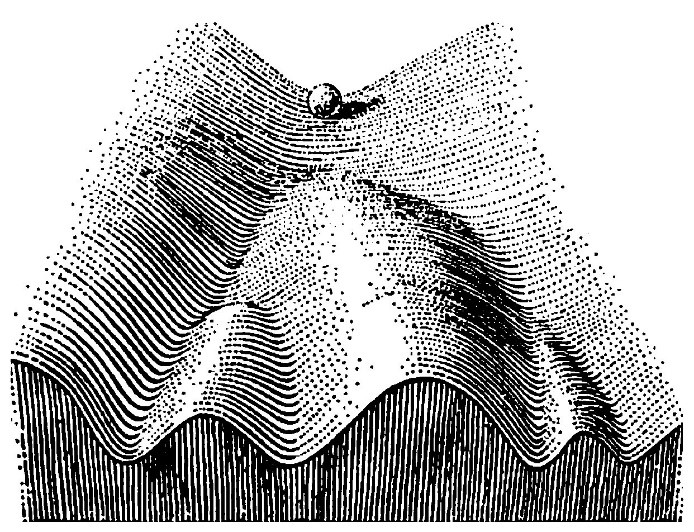
\includegraphics[width=0.5\linewidth,]{figures/intro/waddington} 

}

\caption{Waddington's Classical Epigenetic Landscape}\label{fig:wadd}
\end{figure}
As cells differentiate they acquire a certain identity - controlled by the genes they express and the proteins they produce - which again influences cell `behavior' and its phenotype which includes cell division, migration and cell shape changes. This allows cells to assemble into tissues, which themselves assemble into organs. For developmental biology, which as a scientific discipline originates from embryology, the central interest is to understand how initially inanimate matter (like single atoms and molecules) is able to organize itself to such complex structures we see in living matter at different levels of organismal hierarchy while ensuring a robust developmental plan. Using the marble analogy, studying developmental biology can be thought of tracking multiple cells as they roll down the valley while observing and testing how interactions between them might change their fate. The basic questions arising from this interest are
\begin{itemize}
\tightlist
\item
  How do tissues arise from a population of cells?
\item
  How do organs form from tissues?
\item
  Why do organs form at their particular location?
\item
  How do migrating cells know whether they reached their destination?
\item
  How is growth controlled and how do body axes form?
\end{itemize}
\hypertarget{intro-types}{%
\subsection{Cell Types}\label{intro-types}}

In animals there are two basic types of cells.
\begin{enumerate}
\def\labelenumi{\arabic{enumi}.}
\tightlist
\item
  Epithelial cells, which can form strong adhesions between each other and thereby are able to exert forces upon each other to achieve complex architectures.
\item
  Mesenchymal cells, which do not adhere as strong with each other and are more independent.
\end{enumerate}
This however describes only the extremes on a continuous scale. A cell is not a binary system but can show characteristics of both extremities, e.g.~during Epithelial to Mesenchymal transition (EMT), a bidirectional process whereby epithelial cells can gain migratory and invasive properties and \emph{vice versa}.

A cells identity on this continuum is determined by
\begin{itemize}
\tightlist
\item
  its gene expression profile, which reflects its repertoire of molecular machinery (proteins) and therefore determines its competence to react to internal and external cues.
\item
  its micro-environment, which has a \emph{physical} (forces, energy) and a \emph{chemical} (signaling molecules, diluents) dimension. A change in the latter usually brings about a reaction in the cell which becomes evident both in expression of genes and morphology.
\item
  its shape and incorporation into a tissue, which may modulate how a cell reacts to its micro-environment (e.g.~certain regions of the cell can be more or less exposed, or it can be more or less tightly packed, tuning its susceptibility to forces and signals).
\end{itemize}
With rising numbers of specialized cells assembling into tissue, a shape and body axes begin to emerge that for the earliest developmental stages is highly similar across certain phyla and only begins to diversify at later developmental stages, which reflects our evolutionary ancestry.

\hypertarget{cell-signaling}{%
\subsection{Cell Signaling}\label{cell-signaling}}

To communicate with each other, cells have developed a variety of intercellular communication systems and a complex network of intracellular signal transduction pathways. Some information transfer depends on direct cell-to-cell contact, others rely on freely diffusible ligands that can be sensed by other cells. Each signaling pathway consists of a ligand -- receptor pair that determines their main function. In the following, three pathways are introduced that play major roles in embryonic development.

\hypertarget{wnt}{%
\subsubsection{WNT}\label{wnt}}

The word `WNT' is a compound word of \emph{Wingless} and \emph{Int-1}, both of which are important genes during development of \emph{Drosophila melanogaster} (commonly known as fruit fly), where WNT signaling was first studied. WNT is evolutionary conserved with 15 different receptors and co-receptors and plays a major role during embryonic axis formation, body segmentation, organogenesis and stem cell proliferation. Aberrant WNT signaling is involved in diseases like colon cancer, melanoma and neurodegenerative diseases (\emph{2}).

Beside this, WNT signaling is sub-divided in a canonical (\(\beta\)-catenin\footnote{catenins are regulators of cell-cell adhesion and gene transcription} dependent) and a non-canonical (\(\beta\)-catenin independent) branch. In canonical signaling, WNT ligand binds, together with co-receptor \emph{Lipoprotein Receptor-related Protein 6} (LRP6), to the receptor \emph{Frizzled} (Frz) -- jointly activating protein \emph{Dishevelled} (Dsh). Dsh again inhibits a protein complex usually degrading \(\beta\)-catenin, leading to the stabilization of \(\beta\)-catenin in the cytoplasm and the nucleus. Within the nucleus, \(\beta\)-catenin forms a complex with LEF/TCF to activate specific target genes (\emph{2}).

\hypertarget{intro-FGF}{%
\subsubsection{Fibroblast Growth Factor}\label{intro-FGF}}

Key roles of \emph{Fibroblast growth factor} (FGF) signaling is mesoderm\footnote{one of the earliest differentiating layer of cells. Cells of the mesoderm will e.g.~form the musculature.} patterning in the early embryo, regulation of angiogenesis and wound repair. On a cellular level it is also an important regulator of proliferation and differentiation. The mammalian FGF family is comprised of 18 ligands and four highly conserved transmembrane tyrosine receptors named FGF receptor 1-4 (FGFR1-4). Aberrant FGF signaling is \emph{e.g.} associated with tumor growth (\emph{3}).

Upon ligand binding FGFR dimerizes and undergoes a conformational shift activating the intracellular kinase\footnote{enzymes that transfer energy to specific substrates} domain. Subsequent trans-phosphorylation of tyrosine kinase domains serve as docking sites for adaptor proteins. Activated FGFR then phosphorylates FGFR substrate 2 (FRS2), recruiting adaptor protein \emph{Son of Sevenless} (SoS) and \emph{Growth factor Receptor bound 2} (GRb2) to set on a cascade of at least three possible kinase dependent signal transduction pathways eventually leading to activation of target genes involved in the regulation of e.g.~proliferation, autophagy and EMT (\emph{3}).

\hypertarget{intro-notch}{%
\subsubsection{Notch}\label{intro-notch}}

In neurobiology the term \emph{lateral inhibition} describes the process of an excited neuron reducing the activity of its neighbors. The same principle however can be found in other types of cells too where one cell signals its neighbor cell(s) \emph{not} to acquire a certain fate. For initially equivalent cells to diversify and acquire distinct identities there needs to be a break in symmetry. Often this is accomplished by competition about Notch signaling sources where whichever cell expresses a trait first is able to suppress the same in its surrounding cells. Once this hierarchy is established, it is maintained in a positive feedback manner (\emph{4}, \emph{5}).

Notch signaling gives cells the ability to self-organize and controls various developmental and homeostatic processes that involve patterning, such as sensory hair cell (HC) formation, branched arterial networks or organ morphogenesis. Notch signaling consists of four components:
(1) The extracellular domain of the membrane bound Notch receptor (2) Notch ligands (3) the Notch intracellular domain (NICD) (4) and the \(\gamma\)-Secretase. Upon ligand activation of Notch through Delta, NICD is cleaved and released through \(\gamma\)-Secretase. Subsequently NICD enters the nucleus and together with DNA-binding proteins and co-factors initiates expression of target genes. In contrast to other signaling pathways
\begin{enumerate}
\def\labelenumi{\arabic{enumi}.}
\tightlist
\item
  there are no intermediates between membrane signaling and nucleus and therefore no amplification or dampening of the signal occurs
\item
  signaling requires direct contact between cells, which makes Notch signaling particularly biased by features of cellular morphology and tissue organization (\emph{4}).
\end{enumerate}
Assuming a homogeneous receptor concentration in a cell membrane and since Notch signaling occurs at sites where cells are in contact, the signal generated is proportional to the contact area. Additionally, the strength of the signal increases further where cells are tightly opposed (\emph{4}, \emph{6}--\emph{8}).

\hypertarget{intro-morph}{%
\subsection{Morphogenesis}\label{intro-morph}}

Morphogenesis, from the Greek morphê (shape) and genesis (creation)
\begin{quote}
``Creation of the shape''
\end{quote}
For objects that fulfill a purpose, their form is an expression of their function\footnote{Even though the expression Form follows function (\emph{9}) is usually found in design and architecture, it formulates the general idea that any objects form is (or in design should) be shaped by the requirements to it.}. Analyzing the shape of an object can give information about its function. It is therefore an important feature in different scientific disciplines.

Breaking symmetry of daughter cells often results in one of the daughter cells adopting a different fate, which eventually results in diversification of shape (\emph{e.g.} muscle cells, neural cells, \emph{etc.}). In order to form a tissue or an organ with a variety of specialized cells, it is important for the single cell to have information about where it is located, what its neighbors are doing, how densely it is packed and what the chemical composition of its surrounding is. This is accomplished by being in constant feedback with its neighbor cells and sensation of its environment. After the information got processed, the cell reacts by adjusting the levels of proteins expressed to undergo proliferation or develop specialized structures like cilia or axons.
\begin{quote}
``For an isolated cell, cell shape reflects a balance between cortical tension and intracellular pressure.'' - Y.Pan \emph{et al.}(\emph{10})
\end{quote}
For a cell, its present shape impacts its further specification by defining its ability in perceiving specific signals and the magnitude of signals received and transmitted (\emph{8}). Shape therefore sets the general framework for cell-cell interaction and follows a\newline

\makebox[\linewidth]{$molecular \longrightarrow cellular \longrightarrow tissue$}
\newline

scale hierarchy, where each scale's output again feeds back to the others (figure \ref{fig:feedb}). E.g. it has been shown that simple changes in cell geometry affect fundamental processes such as cell growth, death, direction of cell divisions and extracellular vesicle cargo (\emph{11}--\emph{22}).


\begin{figure}[h]

{\centering 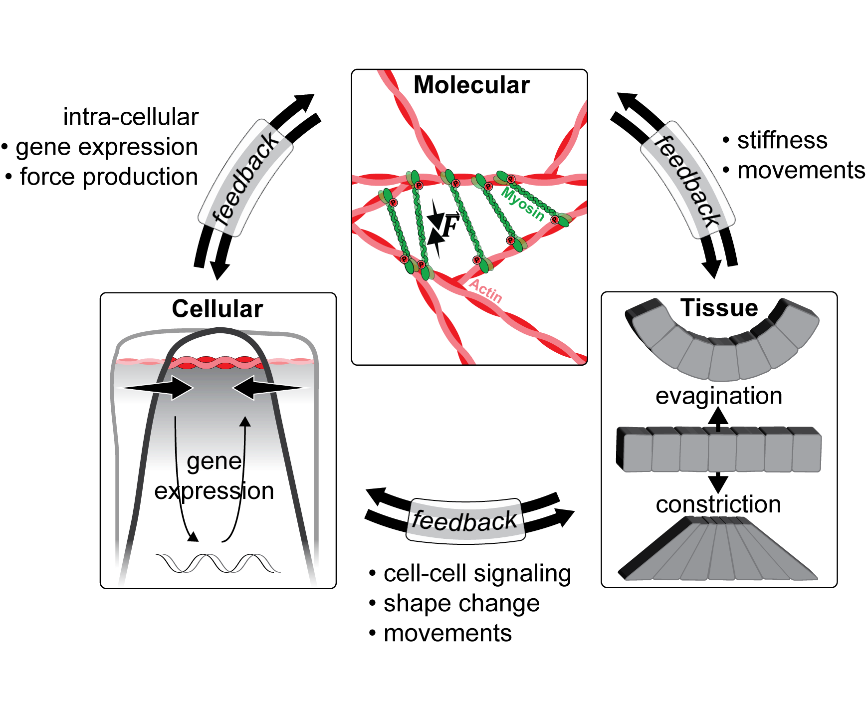
\includegraphics[width=0.85\linewidth,]{figures/intro/feedback} 

}

\caption[Form and function feedback loops]{Form and function feedback loops. On a cellular scale expression of genes may cause a cell to constrict, which again feeds back to the molecular scale (e.g.~force transmission) and the tissue scale (e.g.~evagination or constriction). All of which standing in a continuous feedback.}\label{fig:feedb}
\end{figure}
Cell shape changes may occur in two different ways\ldots{}
\begin{itemize}
\tightlist
\item
  active: Each cell has a dynamic skeleton that is composed of a complex matrix of interconnected proteins - the cytoskeleton. It is composed by three basic classes of filaments that have different physical properties. \emph{Microtubules} (the most rigid), \emph{Intermediate} and \emph{micro-filaments} (the softest). Motor-proteins like Myosin may adhere to actin micro-filaments and contract them, thereby causing e.g.~a narrowing of the cells diameter.
\item
  passive: In a tissue cells are, besides their individual cytoskeletal elements, connected at the supracellular level \emph{via} actin through Adherens junctions. This way, if the tissue becomes deformed at one place, other more distant cells will get deformed as well (\emph{23}).
\end{itemize}
\hypertarget{apical-constriction}{%
\subsubsection{Apical Constriction}\label{apical-constriction}}

Apical constriction (AC) is a cell morphogenetic process manifest by an active narrowing of the apical surface, making an epithelial cell appear bottle or wedge shaped instead of cuboidal. It is usually coordinated by multiple cells within an epithelial layer that raise forces necessary to deform a tissue.

A defining feature of epithelial cells is that they have a basal- (bottom) to apical (top) polarity. At the basal side, the cell is in contact with a variant of extracellular matrix (ECM, a thin sheet-like structure) called the basement membrane, apically the cell forms tight connections to its neighboring cells -- a region called the apical junctional complex (AJC). The AJC encompasses three types of junctions: Adherent junctions (AJ) or zonula adherens (ZA), tight junctions (TJ) and desmosomes. Around the ZA dense cables of actomyosin are located that, analog to muscle sarcomeres, are able to contract upon activation of RHO‑associated protein kinase (Rock) and Rock mediated phosphorylation of the motor protein non-muscle myosin II (NMII) (\emph{24}). The exact mechanism of apical constriction may differ from organism and organ. E.g. it is shown by Martin \emph{et al.} (\emph{25}) that in Drosophila cells are radially organized and RhoA and ROCK have a medioapical focus with RhoA also present at junctions, while Chick cells exhibit a planar cell polarity and RhoGEF and ROCK are localized to junctions.

Developmental processes that involve AC are\ldots{}
\begin{itemize}
\tightlist
\item
  Tissue folding and tube formation
\item
  Single cell ingression and EMT
\item
  Gastrulation
\item
  Healing and sealing of embryonic tissue
\end{itemize}
Epithelial rosettes are radially organized cell clusters within an epithelial tissue whose vertices interface a common center similar to a garlic bud or a pie cut into pieces along its center. While the mechanisms of cytoskeletal rearrangements seem to be well conserved, the signals that lead to rosette formation are less well understood and more diverse.
At least two architectural distinct types of rosettes exist, depending on the tissues polarization.
First, in a planar polarized tissue, several cells converge at a central apico-basal line where cells go from a square to a more triangular shape to form a cylindrical structure (like a pie cut into \(\geq\) 4) (figure \ref{fig:constr}B). Such rosettes are usually observed during tissue elongation and rather short-lived. In a second scenario, cells converge to a central apical point through AC (figure \ref{fig:constr}A). This type of rosette is more long-lived and usually does not resolve but already represents a morphologically pre-mature state of the organ to be formed (\emph{26}).


\begin{figure}

{\centering 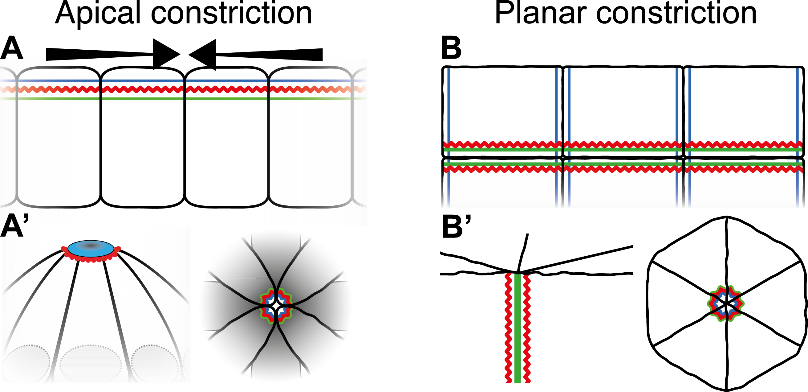
\includegraphics[width=0.6\linewidth]{figures/intro/constriction} 

}

\caption[Modes of constriction]{Modes of constriction. \textbf{A} Cells converge to a central apical point \textbf{B} Cells converge at a central apico-basal line.}\label{fig:constr}
\end{figure}
\hypertarget{model-organism-and-system}{%
\section{Model Organism and System}\label{model-organism-and-system}}

To study biological phenomena, biologists use a variety of non-human model organisms. While each model organism has its advantages and disadvantages, the choice for a model depends on the scientific question.

To study embryonic development the fresh water fish \emph{Danio rerio} (also known as eng: \emph{zebrafish} or \emph{ger:} zebrabärbling (figure\ref{fig:zebra})) has become an important model organism over the recent years. \emph{D.rerio} is a diploid organism with a fully sequenced genome (of the human genes 71.4\% have at least one \emph{D.rerio} ortholog, 47\% have a one-to-one ortholog (\emph{27}). It has a relatively short alternation of generations (12-16 weeks), a regularly large number of embryos (100 / week / female) and is relatively undemanding in terms of space for breeding. Furthermore, it offers well-established methods for mutagenesis, screening, and generation of transgenic lines. Since its embryos are naturally transparent and develop externally, it is an ideal system for microscopic examination using molecular dyes and tags to visualize \emph{inter} and \emph{intra} cellular components even deep within the tissue (e.g.~cell nuclei or cell membrane fluorescent tags). Together with advances in imaging techniques, this also allows for high-throughput, high-resolution, long-term \emph{in vivo} imaging. Especially the expression of fluorescent proteins in a tissue- or organ-specific manner in transparent embryos offers enormous possibilities to address interesting and long-standing open questions.

In nature, zebrafish can be found in the shallow waters of the Indian and Pakistan Ganges inflows. It exhibits an oval body shape and can reach a length of up to 5 cm in adulthood. While females are usually more silverish, males have a brownish back and a yellow-whit belly. Laterally it exhibits its name-giving dark-blue iridescent stripes with silver in between.


\begin{figure}

{\centering 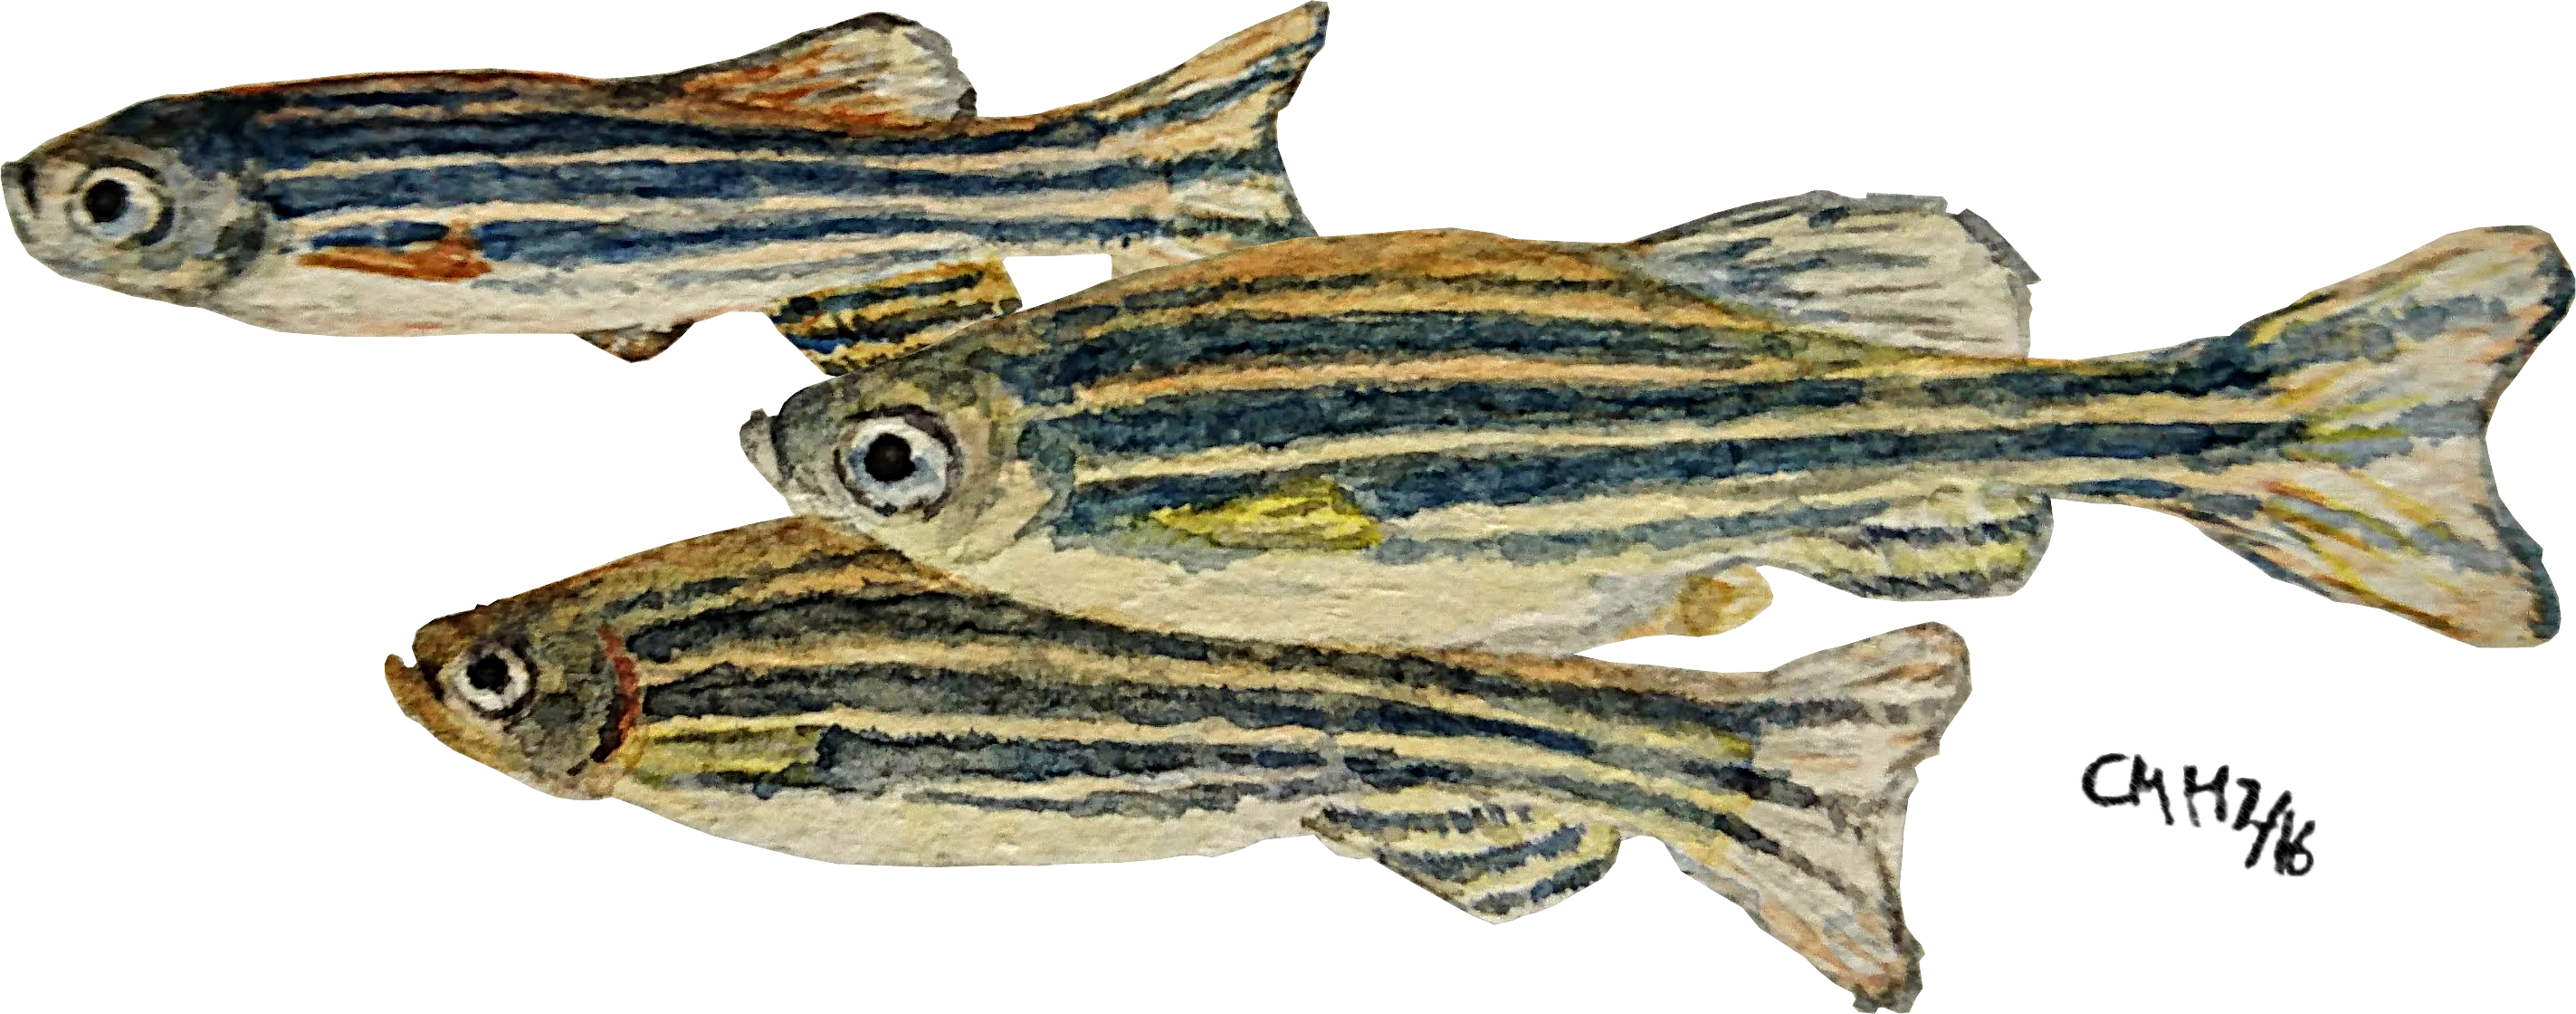
\includegraphics[width=0.5\linewidth]{figures/intro/CM_fish} 

}

\caption[Model organism Danio rerio]{Model organism \emph{Danio rerio} (aquarell by Christine Molenda)}\label{fig:zebra}
\end{figure}
\hypertarget{developmental-stages}{%
\subsection{Developmental Stages}\label{developmental-stages}}

A single female may lay 100 eggs per week. Each Zygote\footnote{first diploid cell after fertilization} then undergoes the first zygotic cell cycle (\textbf{at \textasciitilde{} 0.75 h}). The following two to seven cell cycles (period: \emph{Cleavage}, \textbf{at \textasciitilde{} 2.25 h}) occur directed and synchronous every \textasciitilde15 min. Cells in this stage are called \emph{blastomeres}, are incompletely separated from the yolk and remain interconnected by cytoplasmic bridges. The \emph{Blastula} period (\textbf{up to 5.25 h}) is determined by increasingly asynchronous division, flattening of the blastoderm \emph{via} cell intercalation and lengthening of the cell cycle. This period is also marked by the onset of \emph{epiboly}, the period when cells in late blastula start to dome while a monolayer of the domes circumfence begins to wrap around the Yolk (\emph{28}).

After Blastula and \textbf{until 10 h} the \emph{Gastrula} period takes place, followed by the \emph{Segmentation} period (\textbf{until 24 h}). Both of which are depicted in more detail in figure \ref{fig:stages}. At even later stages the embryo starts to elongate posteriorly, grow and develop organs until it first active muscle are present and it starts to swim (figure \ref{fig:stages}).


\begin{figure}

{\centering \includegraphics[width=0.95\linewidth]{figures/intro/stages} 

}

\caption[Zebrafish embryonic development]{Zebrafish embryonic development. Microscopic images are from a time-lapse where 24 embryos were imaged simultaneously in brightfield and at 488 nm Z-Stacks. Representation shows contrast enhanced EDFs. Bottom row (30-48 hpf) stages are handmade drawings from live embryos made during the first week of my PhD.}\label{fig:stages}
\end{figure}
\hypertarget{the-lateral-line-system}{%
\subsection{The Lateral Line System}\label{the-lateral-line-system}}

The lateral line (LL) system is a mechano-sensory organ that is common to all aquatic vertebrates and evolutionary remnants could even be found in mice (\emph{29}). It enables the animal to sense water movements and therefore to orient itself, and to detect prey and predators. Fully developed, the lateral line system is comprised of hundreds of neuromasts positioned in an orderly pattern all over the animal's body (figure \ref{fig:llsystem}A). Its functional subunits are the neuromasts (NM) (figure \ref{fig:llsystem}B-C) that, when fully developed, consist of hair-, support- and mantle cells. To sense water movements, each NM projects kino- and stereo-cilia out of the skin that, upon water induced deflection, generate action potentials that are transduced \emph{via} afferent fibers (\emph{30}, \emph{31}).


\begin{figure}

{\centering 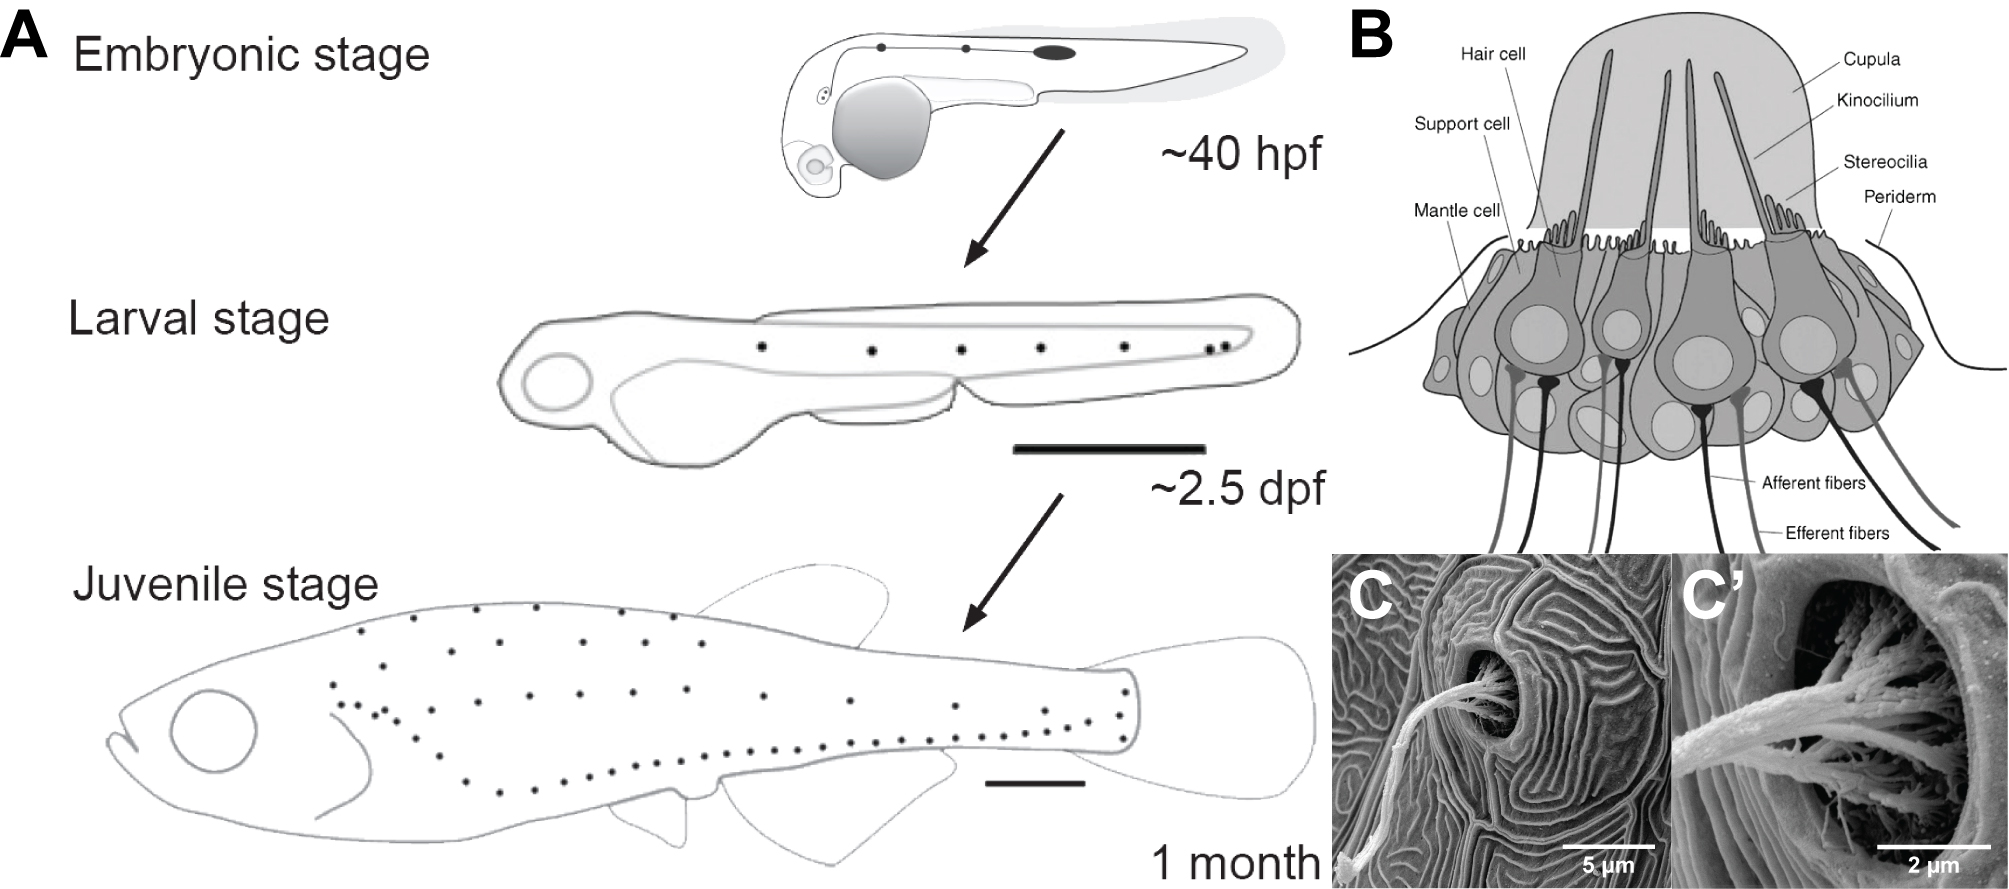
\includegraphics[width=0.85\linewidth]{figures/intro/ll_system} 

}

\caption[The lateral line system]{The lateral line system. \textbf{A} modified after (Ghysen \emph{et al.}, 2012) and A.Bergs, 2016 (student presentation at AK Lecaudey). Development of the later line system at embryonic, larval and juvenile stage. \textbf{B} Schematic showing a crossection and organization of a single neuromast. \textbf{C-C'} SEM images of a single, pre-mature (3 dpf) neuromast.}\label{fig:llsystem}
\end{figure}
Each NM is first deposited as a premature cluster of about 30 cells from a migrating cell-aggregate called the posterior lateral line primordium (pLLP) (figure \ref{fig:llgfp}A). The pLLP delaminates from the pLL placode, caudal to the otic vesicle (figure \ref{fig:llgfp}B) at around 20 \emph{hours post fertilization} (hpf) as a group of \textasciitilde100 cells. After formation of a mesenchymal-like leading region, it starts migrating along a chemokine gradient positioned at the horizontal myoseptum to the tip of the tail (\emph{30}, \emph{31}). To ensure the development of a functional organ, several fundamental biological processes like cell migration, morphogenesis, proliferation and cell polarization need to be integrated into the pLLP.
An important breakthrough in LL research has been the development of a transgenic line expressing a membrane tethered GFP fusion protein (lyn-GFP) that is expressed under the LL specific promotor of \emph{cldnb} (claudin b\footnote{construct name: \emph{Tg(-8.0cldnb:lynGFP)}; ZFIN ID: ZDB-TGCONSTRCT-070117-15}) (\emph{32}), which allows for a much more detailed view and to observe lateral line development \emph{in vivo}. An example of the fluorescence signal visible at \textasciitilde60 hpf can be seen in figure \ref{fig:llgfp}B.


\begin{figure}

{\centering 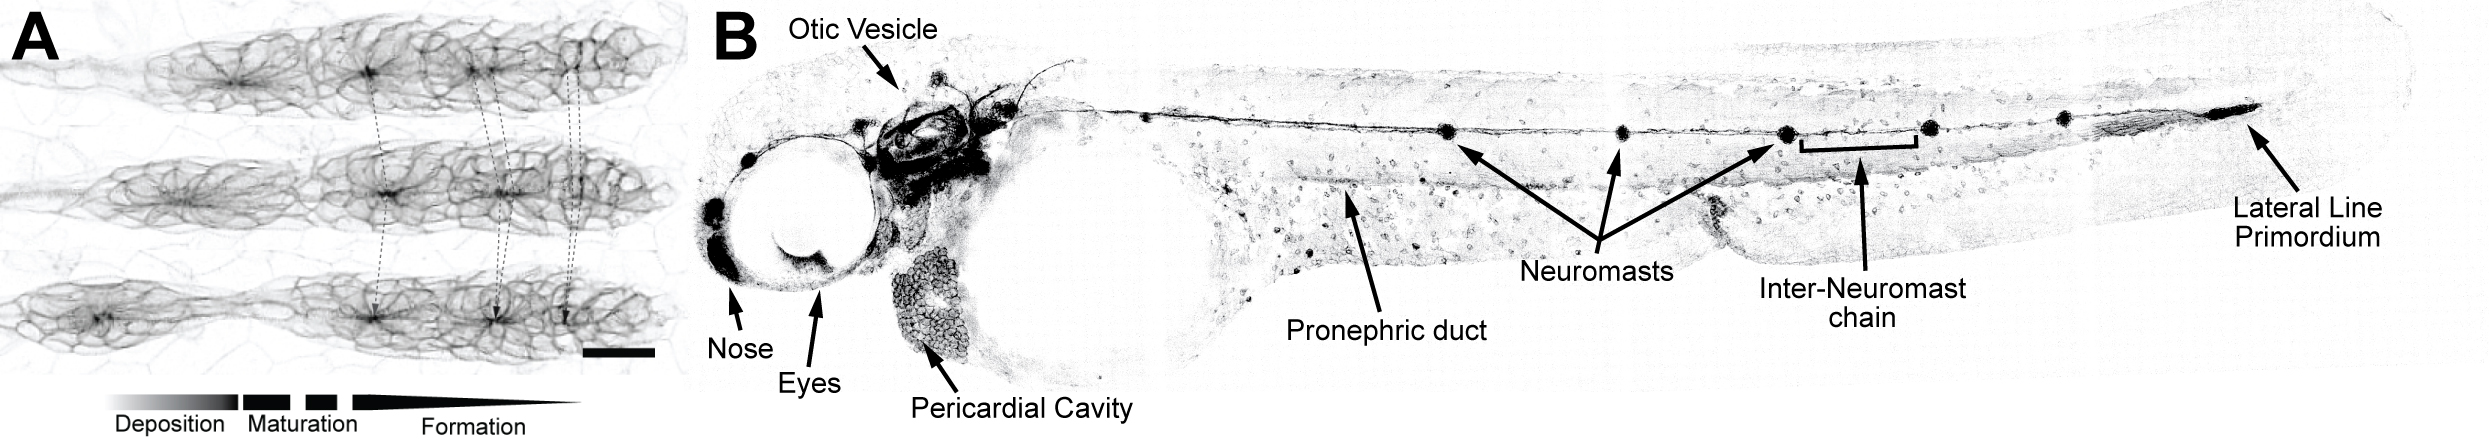
\includegraphics[width=0.95\linewidth]{figures/intro/ll_gfp} 

}

\caption[Neuromast deposition and pattern]{Neuromast deposition and pattern. \textbf{A} Scheme showing NM deposition over three timepoints (10 min. interval). Dotted lines are time-tracks of rosettes, which become more concentrated over time. Bottom arrow indicates regions of rosette formation, maturation and deposition within the pLLP (scale bar = 20 µm; 20X WI; \textasciitilde20 Z-planes; 2.5 µm spacing. MaxIP. Colors inverted.) \textbf{B} Scheme showing the lateral line at end of migration (\textasciitilde60 hpf) and other parts visible through the cldnb:lyn-gfp transgene (as documented through zfin.org) (air objective + 1.5X tube lens; four tiles; \textasciitilde20 Z-planes; 5 µm spacing. MaxIP. Colors inverted).}\label{fig:llgfp}
\end{figure}
\hypertarget{posterior-lateral-line-primordium}{%
\subsection{Posterior Lateral Line Primordium}\label{posterior-lateral-line-primordium}}

The pLLP is about 100-150 \(\mu\)m in length (depending on deposition cycle) over which it exhibits a diverse surface topology and cellular morphology. Previous research found that the \emph{caudal} (also \emph{posterior}), more mesenchymal cells, are leading the path of migration, while the \emph{cranial} (also \emph{anterior}), more epithelial cells, are trailing. Towards the leading region the cells are more flat, towards the trailing region the cells become more columnar and increasingly radially organized into formations called epithelial rosettes. During migration the pLLP typically contains 2-3 \emph{rosettes} (\textasciitilde25-30 cells each), while the most trailing one will eventually be deposited to further mature to a functional NM (\emph{30}, \emph{33}). Every deposition comes with a loss of cells in the pLLP, but this loss is partially compensated by proliferation during migration. While one study concludes a general spatial heterogeneity in distribution of proliferative cells (\emph{34}), another one suggests a higher proliferative rate specifically near the leading region (\emph{35}).

\hypertarget{rosette-formation}{%
\subsubsection{Rosette formation}\label{rosette-formation}}

The onset of morphological and functional changes is determined by signaling of FGF, which is mostly active in the trailing region. Causal for expression of FGF is a signaling center of WNT in the leading region, which promotes expression of FGF ligands \emph{Fgf-3} and \emph{-10} (\emph{36}). Those ligands then diffuse to the trailing domain where binding through \emph{FGF receptor 1} (Fgfr1) triggers a signaling cascade through which the cells become more columnar, apically constricted and eventually re-organize into epithelial rosettes (\emph{35}, \emph{37}, \emph{38}). Concurrently, cells of the WNT signaling center themselves are not competent to FGF signaling, which is achieved through expression of \emph{Sef}, an intracellular antagonist to Fgfr1 signaling (\emph{39}).

It was shown that rosette formation in the lateral line primordium (LLP) is an important morphological feature for a lumen to form on top of the rosette which, filled with FGF, acts as a locally enriched source of FGF signaling (\emph{40}).

\hypertarget{intro-atoh}{%
\subsubsection{Hair cell specification}\label{intro-atoh}}

Downstream of FGF lies the expression of the transcription factor (TF) Atoh1a, which gives cells the potential to become sensory HCs (\emph{35}).

The current model suggests that
\begin{enumerate}
\def\labelenumi{\arabic{enumi}.}
\tightlist
\item
  FGF initiates expression of \emph{atoh1a} and \emph{deltaA}, where DeltaA activates Notch in neighboring cells to inhibit expression of \emph{atoh1a} in those.
\item
  Atoh1a in turn suppresses competence for FGF and initiates expression of \emph{atoh1b} and \emph{deltaD} which act synergistically with DeltaA in the center cell of the forming rosette.
\item
  While the latter acts synergistic with DeltaA, Atoh1b in turn drives expression of \emph{atoh1a} (\emph{41}).
\item
  Once a prospective HC is specified it will itself become a source for Fgf-10. By this process adjacent cells are laterally inhibited and determined as \emph{support cells} (figure \ref{fig:llsystem}B), still capable of receiving FGF signals \emph{via} Fgfr1.
\end{enumerate}
Just before the most trailing rosette is deposited, its prospective HC will undergo a final division to form a doublet of sensory HCs (\emph{42}, \emph{43}).

\hypertarget{shroom3-in-the-pllp}{%
\subsection{Shroom3 in the pLLP}\label{shroom3-in-the-pllp}}

The Shroom protein family is mostly conserved through animal evolution (figure \ref{fig:suppshrmort}) and involved in contraction of the actomyosin network (e.g.~during AC), which has been confirmed in several studies investigating \emph{e.g.} epithelial planar remodeling, neural tube morphogenesis and \emph{Xenopus} bottle cells (\emph{44}--\emph{49}).

\hypertarget{intro-shroom}{%
\subsubsection{Recent research}\label{intro-shroom}}

Shroom proteins have three characteristic domains (1) a \emph{PDZ} domain close to the N-terminus to interact with other proteins with PDZ-binding domains and (2) two \emph{Apx/Shroom} domains (ASD-1 and -2), the latter being close to the proteins C-terminus. The Shroom domains may interact with proteins containing a \emph{Shroom binding domain} (SBD) such as Rock to help and facilitate phosphorylation of NMII (figure \ref{fig:shrminteract}) (\emph{50}).


\begin{figure}

{\centering 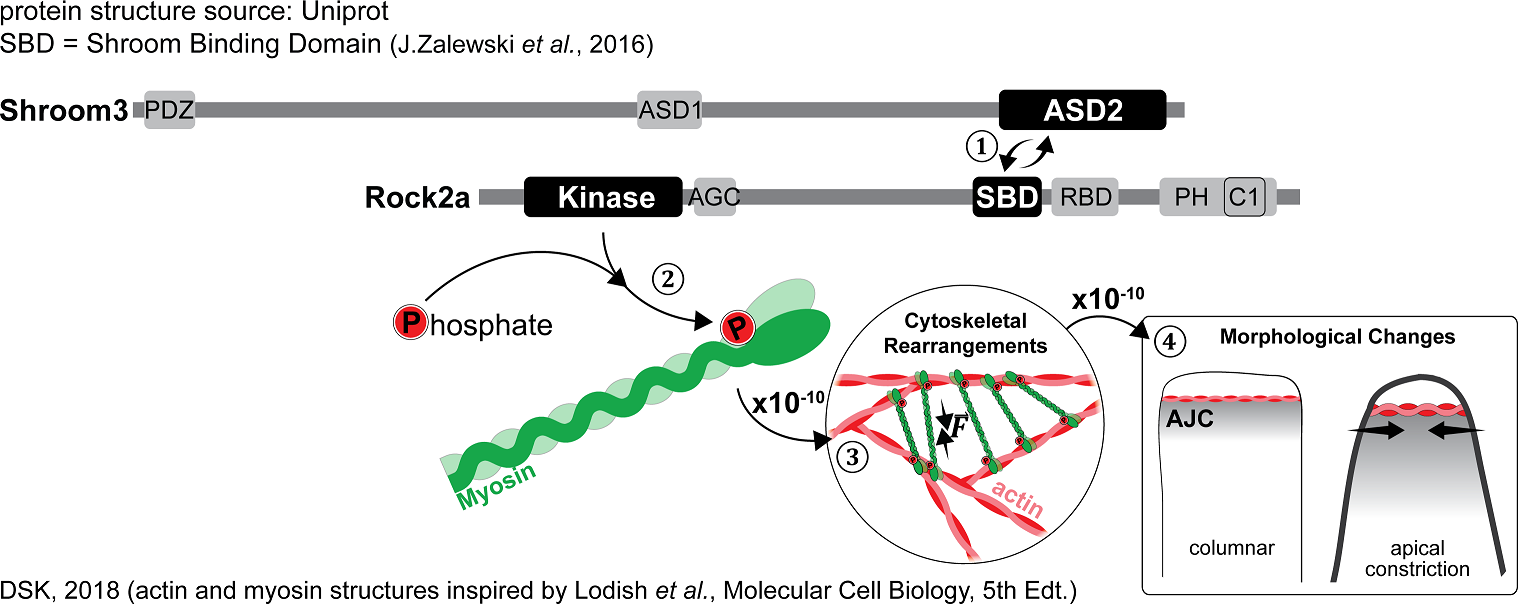
\includegraphics[width=0.95\linewidth]{figures/intro/shrm3_interaction} 

}

\caption[Shroom3 functional domains and mode of operation]{Shroom3 functional domains and mode of operation. Sequence of events numbered from 1-4. Approximate scale jumps indicated at arrows.}\label{fig:shrminteract}
\end{figure}
While in all of the above-mentioned studies Shroom3 was the focus of interest, in zebrafish and most other model organisms there are four paralogs. A previous study performed by a lab-mate done on Shroom3 morphants in \emph{D.rerio} (\emph{1}) indicates that Shroom3 is also necessary for AC and rosette formation in the migrating pLLP. In summary she was able to show that\ldots{}
\begin{enumerate}
\def\labelenumi{\arabic{enumi}.}
\tightlist
\item
  Shroom3 is expressed in the pLLP from stages 24 -- 48 hpf.
\item
  \emph{shroom3} is expressed downstream of FGF signaling, which was shown \emph{via} treatment with an Fgfr inhibiting drug.
\item
  Shroom3 localizes to rosette centers, which was accomplished by generating a transgenic line expressing a \emph{shroom3-tagRFP} fusion protein under the control of a heat-shock\footnote{heat shock proteins are \emph{Escherichia coli} enzymes that assist protein folding and are heat activated} promotor (figure \ref{fig:shrmernst}A).
\item
  Rosette formation is impaired in MO injected embryos, which was shown quantitatively by using a specifically trained \emph{rosette detector} (\emph{51}) to count and weight single rosettes.
\end{enumerate}

\begin{figure}

{\centering 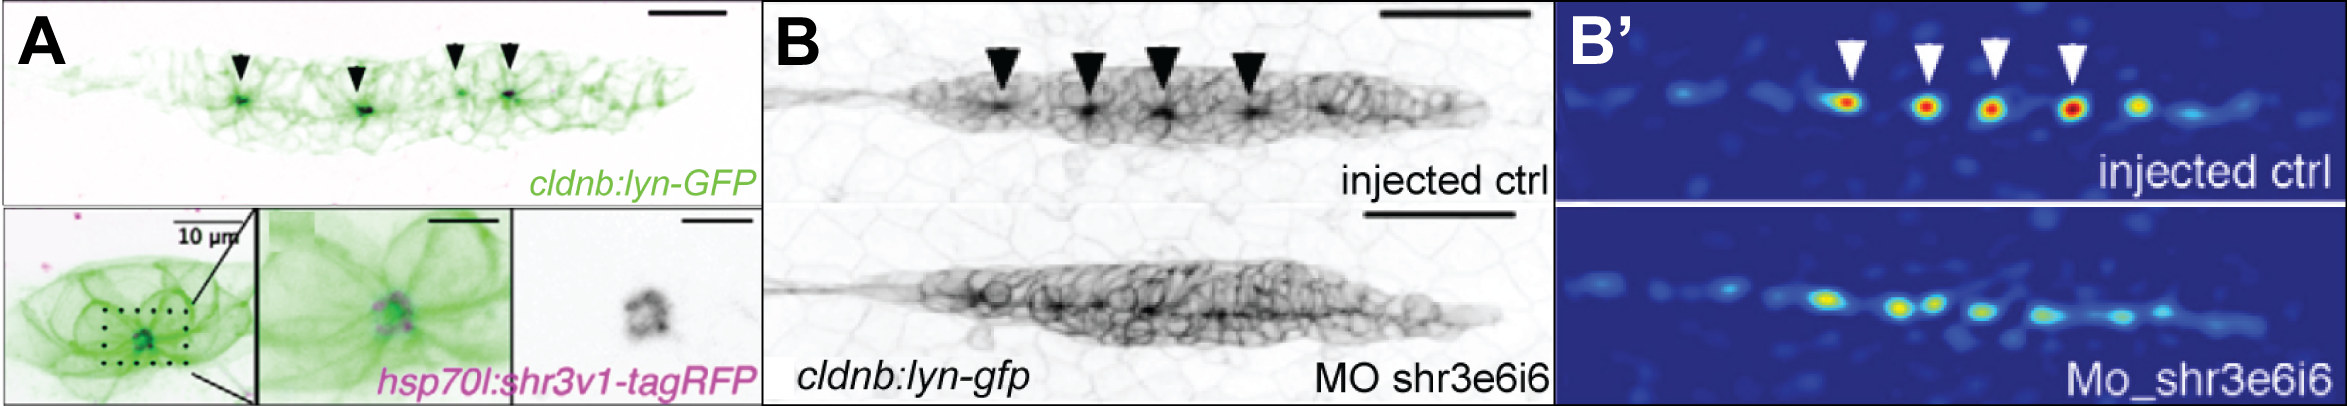
\includegraphics[width=0.95\linewidth]{figures/intro/shrm_ernst} 

}

\caption[Shroom3 in rosette formation]{Shroom3 in rosette formation (adapted from Ernst et al., 2012) \textbf{A} composite MaxIPs of membrane label and fusion protein showing the localization of Shroom within the pLLP \textbf{B} uninjected control and shroom3 MO injected MaxIPs \textbf{B'} Heat-maps of rosette detector score.}\label{fig:shrmernst}
\end{figure}
\hypertarget{current-model}{%
\subsubsection{Current Model}\label{current-model}}

Based on these and previous results, the current model for apical constriction in the pLLP assumes that (1) expression of \emph{shroom3} is induced by FGF signaling (2) Shroom3 binds Rock and translocates it to the AJC to (3) mediate phosphorylation of NMII which (3) induces contraction of the actin network and AC (figure \ref{fig:shrmmodel}). Furthermore, AC is necessary for rosette assembly and subsequent NM deposition. In conclusion the current understanding is that without Shroom3 AC and rosette formation are impaired, leading to a defect in NMs and NM deposition.


\begin{figure}[h]

{\centering 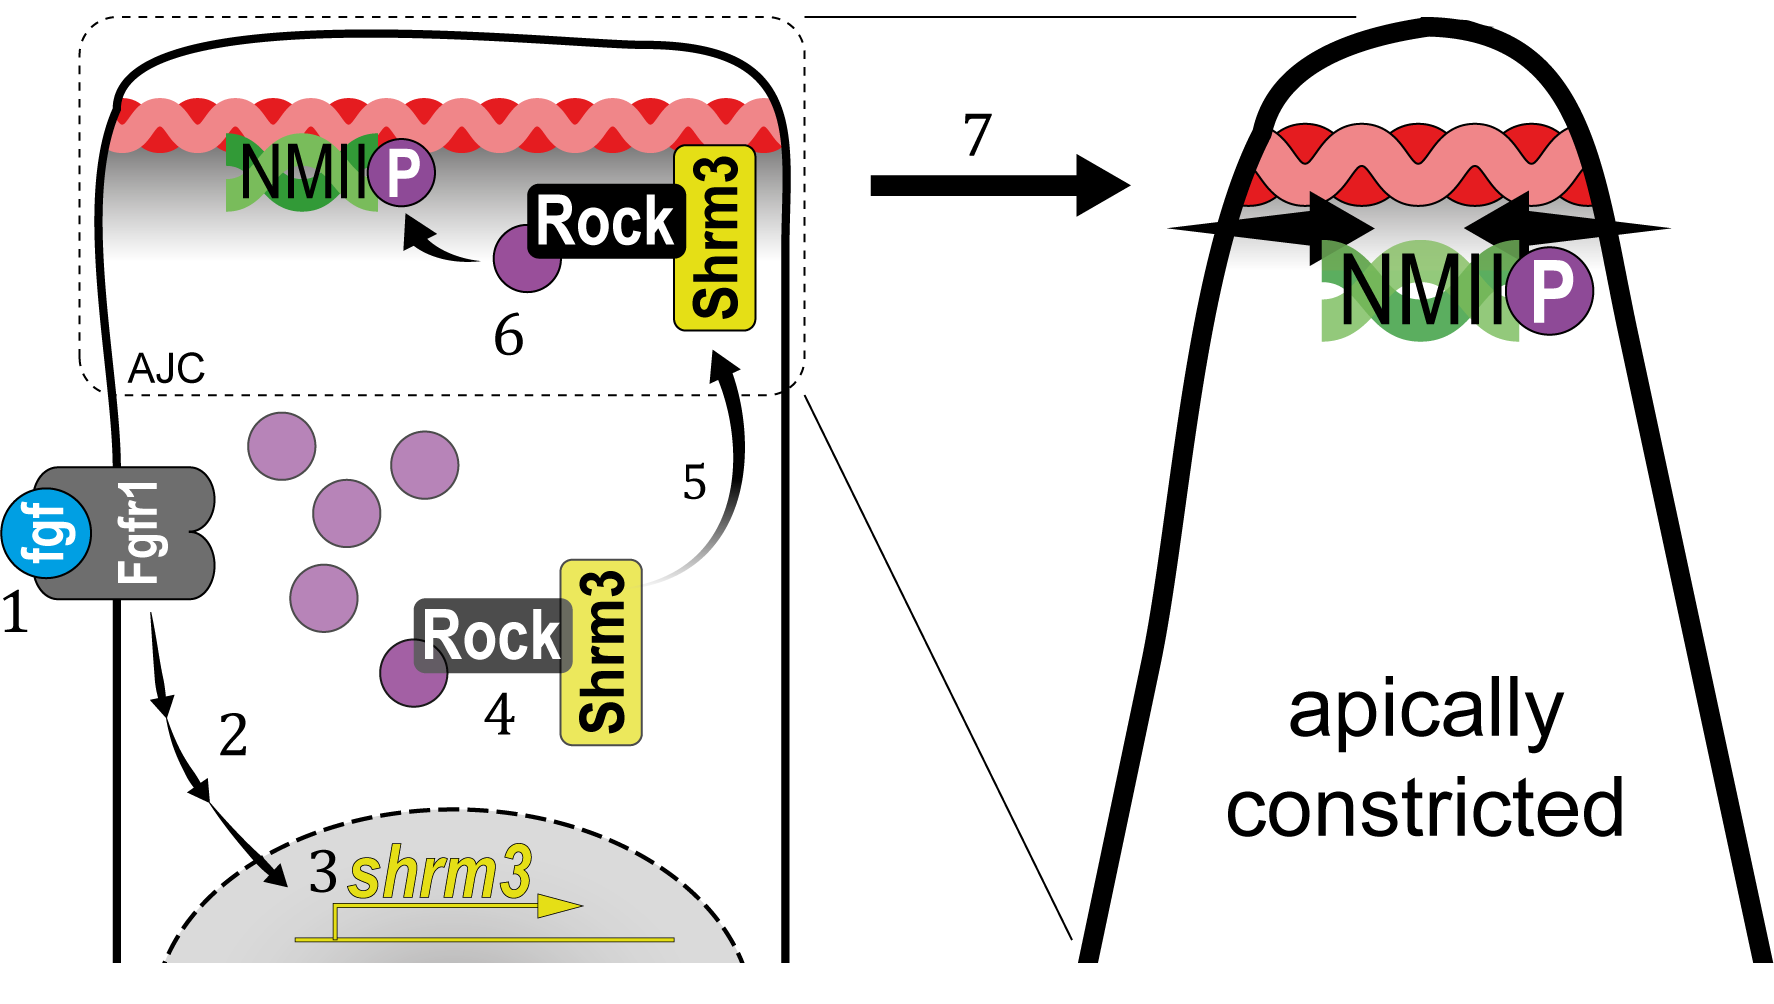
\includegraphics[width=0.5\linewidth,]{figures/intro/shrm_model} 

}

\caption{Shroom3 current model}\label{fig:shrmmodel}
\end{figure}
\hypertarget{shroom3-mutants}{%
\subsection{\texorpdfstring{\emph{shroom3} mutants}{shroom3 mutants}}\label{shroom3-mutants}}

Morpholino injection allows transient gene knockdown in various species which has been broadly used over recent years. Although they have been and are still a useful tool for the zebrafish community, there are a number of limitations.

Those include\ldots{}
\begin{itemize}
\tightlist
\item
  they need to be injected for each experiment. Even if the person injecting is well trained, there is always some loss in embryos. Furthermore, injection leads to a delay in development
\item
  the induction of non-specific phenotypes due to activation of, among others, p53-mediated cell death.
\item
  the degradation of the morpholino, which allows to analyze the phenotype over a limited period of time only (3 to 5 days after injection)
\end{itemize}
Because of these limitations, a former colleague in the lab had generated a mutant once it became technically possible using Transcription activator-like effector nuclease (TALEN) to confirm and further study the role of Shroom3 during morphogenesis. An 8 bp deletion in the SD2 domain was isolated and maintained as a stable line. This mutation leads to a premature STOP codon disrupting the SD2 domain, thereby inhibiting Shroom3's function.

While birth rates follow a distribution of Mendelian inheritance (after genotyping at 3 months of age), mutant adults have a shortened lifespan (\textasciitilde6-9 months). Shroom3 mutants are morphologically similar to their siblings, however their gill flaps seem to be increased in size, swollen, and not exactly streamlined with the body. This is also evident by an increased frequency of gill flap beating. Like the MO injected embryos, in a first qualitative analysis of the phenotype the pLLP exhibits a noticeable defect in rosette assembly. To our surprise however, the number of NMs deposited at the end of migration was significantly increased in the mutants as compared to the controls.

\hypertarget{open-questions-and-motivation}{%
\section{Open Questions and Motivation}\label{open-questions-and-motivation}}

The main objectives of my thesis were\ldots{}
\begin{enumerate}
\def\labelenumi{\arabic{enumi}.}
\tightlist
\item
  a complete characterization of the newly generated \emph{shroom3} mutant phenotype till 5 dpf
\item
  development of methodology for an automated, more precise, higher throughput and less invasive quantification of pLLP and LL phenotypes
\item
  to use the mutant phenotype to better understand the relationship between rosette assembly and NM deposition
\item
  to analyze the feedback between morphological changes (apical constriction and mediated rosette assembly) and cell fate specification in the pLLP.
\end{enumerate}
\hypertarget{mat-met}{%
\chapter{Materials and Methods}\label{mat-met}}

\hypertarget{mat}{%
\section{Materials}\label{mat}}

\hypertarget{mat-chem}{%
\subsection{Chemicals}\label{mat-chem}}
\begin{longtable}[]{@{}rcl@{}}
\caption{\label{tab:met-chem} Chemicals}\tabularnewline
\toprule
\begin{minipage}[b]{0.29\columnwidth}\raggedleft
Chemical\strut
\end{minipage} & \begin{minipage}[b]{0.33\columnwidth}\centering
Company\strut
\end{minipage} & \begin{minipage}[b]{0.29\columnwidth}\raggedright
cat.-no.\strut
\end{minipage}\tabularnewline
\midrule
\endfirsthead
\toprule
\begin{minipage}[b]{0.29\columnwidth}\raggedleft
Chemical\strut
\end{minipage} & \begin{minipage}[b]{0.33\columnwidth}\centering
Company\strut
\end{minipage} & \begin{minipage}[b]{0.29\columnwidth}\raggedright
cat.-no.\strut
\end{minipage}\tabularnewline
\midrule
\endhead
\begin{minipage}[t]{0.29\columnwidth}\raggedleft
Agarose\strut
\end{minipage} & \begin{minipage}[t]{0.33\columnwidth}\centering
Roth\strut
\end{minipage} & \begin{minipage}[t]{0.29\columnwidth}\raggedright
6351.2\strut
\end{minipage}\tabularnewline
\begin{minipage}[t]{0.29\columnwidth}\raggedleft
Agar-Agar\strut
\end{minipage} & \begin{minipage}[t]{0.33\columnwidth}\centering
Roth\strut
\end{minipage} & \begin{minipage}[t]{0.29\columnwidth}\raggedright
5210.3\strut
\end{minipage}\tabularnewline
\begin{minipage}[t]{0.29\columnwidth}\raggedleft
Ampicillin\strut
\end{minipage} & \begin{minipage}[t]{0.33\columnwidth}\centering
Roth\strut
\end{minipage} & \begin{minipage}[t]{0.29\columnwidth}\raggedright
K029.2\strut
\end{minipage}\tabularnewline
\begin{minipage}[t]{0.29\columnwidth}\raggedleft
ATP\strut
\end{minipage} & \begin{minipage}[t]{0.33\columnwidth}\centering
Epicentre\strut
\end{minipage} & \begin{minipage}[t]{0.29\columnwidth}\raggedright
E311K\strut
\end{minipage}\tabularnewline
\begin{minipage}[t]{0.29\columnwidth}\raggedleft
Blocking Reagent\strut
\end{minipage} & \begin{minipage}[t]{0.33\columnwidth}\centering
Roche\strut
\end{minipage} & \begin{minipage}[t]{0.29\columnwidth}\raggedright
11096176001\strut
\end{minipage}\tabularnewline
\begin{minipage}[t]{0.29\columnwidth}\raggedleft
BCIP\strut
\end{minipage} & \begin{minipage}[t]{0.33\columnwidth}\centering
Fermentas\strut
\end{minipage} & \begin{minipage}[t]{0.29\columnwidth}\raggedright
R0822\strut
\end{minipage}\tabularnewline
\begin{minipage}[t]{0.29\columnwidth}\raggedleft
CaCl\textsubscript{2}\strut
\end{minipage} & \begin{minipage}[t]{0.33\columnwidth}\centering
Roth\strut
\end{minipage} & \begin{minipage}[t]{0.29\columnwidth}\raggedright
886.1\strut
\end{minipage}\tabularnewline
\begin{minipage}[t]{0.29\columnwidth}\raggedleft
Calyculin\strut
\end{minipage} & \begin{minipage}[t]{0.33\columnwidth}\centering
Sigma\strut
\end{minipage} & \begin{minipage}[t]{0.29\columnwidth}\raggedright
208851\strut
\end{minipage}\tabularnewline
\begin{minipage}[t]{0.29\columnwidth}\raggedleft
DAPI\strut
\end{minipage} & \begin{minipage}[t]{0.33\columnwidth}\centering
Sigma\strut
\end{minipage} & \begin{minipage}[t]{0.29\columnwidth}\raggedright
D9542\strut
\end{minipage}\tabularnewline
\begin{minipage}[t]{0.29\columnwidth}\raggedleft
DIG RNA Mix\strut
\end{minipage} & \begin{minipage}[t]{0.33\columnwidth}\centering
Roche\strut
\end{minipage} & \begin{minipage}[t]{0.29\columnwidth}\raggedright
11277073910\strut
\end{minipage}\tabularnewline
\begin{minipage}[t]{0.29\columnwidth}\raggedleft
DMSO\strut
\end{minipage} & \begin{minipage}[t]{0.33\columnwidth}\centering
Roth\strut
\end{minipage} & \begin{minipage}[t]{0.29\columnwidth}\raggedright
4720.2\strut
\end{minipage}\tabularnewline
\begin{minipage}[t]{0.29\columnwidth}\raggedleft
EtBr\strut
\end{minipage} & \begin{minipage}[t]{0.33\columnwidth}\centering
Roth\strut
\end{minipage} & \begin{minipage}[t]{0.29\columnwidth}\raggedright
2218.3\strut
\end{minipage}\tabularnewline
\begin{minipage}[t]{0.29\columnwidth}\raggedleft
EtOH\strut
\end{minipage} & \begin{minipage}[t]{0.33\columnwidth}\centering
Roth\strut
\end{minipage} & \begin{minipage}[t]{0.29\columnwidth}\raggedright
9065.3\strut
\end{minipage}\tabularnewline
\begin{minipage}[t]{0.29\columnwidth}\raggedleft
Formaldehyde\strut
\end{minipage} & \begin{minipage}[t]{0.33\columnwidth}\centering
Roth\strut
\end{minipage} & \begin{minipage}[t]{0.29\columnwidth}\raggedright
7398.1\strut
\end{minipage}\tabularnewline
\begin{minipage}[t]{0.29\columnwidth}\raggedleft
Formamide\strut
\end{minipage} & \begin{minipage}[t]{0.33\columnwidth}\centering
Roth\strut
\end{minipage} & \begin{minipage}[t]{0.29\columnwidth}\raggedright
P040.1\strut
\end{minipage}\tabularnewline
\begin{minipage}[t]{0.29\columnwidth}\raggedleft
Glycerol\strut
\end{minipage} & \begin{minipage}[t]{0.33\columnwidth}\centering
Roth\strut
\end{minipage} & \begin{minipage}[t]{0.29\columnwidth}\raggedright
3783.2\strut
\end{minipage}\tabularnewline
\begin{minipage}[t]{0.29\columnwidth}\raggedleft
IPTG\strut
\end{minipage} & \begin{minipage}[t]{0.33\columnwidth}\centering
Thermo\strut
\end{minipage} & \begin{minipage}[t]{0.29\columnwidth}\raggedright
R1171\strut
\end{minipage}\tabularnewline
\begin{minipage}[t]{0.29\columnwidth}\raggedleft
KCl\strut
\end{minipage} & \begin{minipage}[t]{0.33\columnwidth}\centering
Roth\strut
\end{minipage} & \begin{minipage}[t]{0.29\columnwidth}\raggedright
P017.1\strut
\end{minipage}\tabularnewline
\begin{minipage}[t]{0.29\columnwidth}\raggedleft
Low melting point Agarose\strut
\end{minipage} & \begin{minipage}[t]{0.33\columnwidth}\centering
Roth\strut
\end{minipage} & \begin{minipage}[t]{0.29\columnwidth}\raggedright
A9539\strut
\end{minipage}\tabularnewline
\begin{minipage}[t]{0.29\columnwidth}\raggedleft
Maleic Acid\strut
\end{minipage} & \begin{minipage}[t]{0.33\columnwidth}\centering
Roth\strut
\end{minipage} & \begin{minipage}[t]{0.29\columnwidth}\raggedright
3810.3\strut
\end{minipage}\tabularnewline
\begin{minipage}[t]{0.29\columnwidth}\raggedleft
MgSO\textsubscript{4}\strut
\end{minipage} & \begin{minipage}[t]{0.33\columnwidth}\centering
Roth\strut
\end{minipage} & \begin{minipage}[t]{0.29\columnwidth}\raggedright
T888.2\strut
\end{minipage}\tabularnewline
\begin{minipage}[t]{0.29\columnwidth}\raggedleft
MeOH\strut
\end{minipage} & \begin{minipage}[t]{0.33\columnwidth}\centering
Roth\strut
\end{minipage} & \begin{minipage}[t]{0.29\columnwidth}\raggedright
CP43.3\strut
\end{minipage}\tabularnewline
\begin{minipage}[t]{0.29\columnwidth}\raggedleft
MgCl\textsubscript{2}\strut
\end{minipage} & \begin{minipage}[t]{0.33\columnwidth}\centering
Roth\strut
\end{minipage} & \begin{minipage}[t]{0.29\columnwidth}\raggedright
2189.1\strut
\end{minipage}\tabularnewline
\begin{minipage}[t]{0.29\columnwidth}\raggedleft
NaCl\strut
\end{minipage} & \begin{minipage}[t]{0.33\columnwidth}\centering
Roth\strut
\end{minipage} & \begin{minipage}[t]{0.29\columnwidth}\raggedright
9265.2\strut
\end{minipage}\tabularnewline
\begin{minipage}[t]{0.29\columnwidth}\raggedleft
NaHCO\textsubscript{3}\strut
\end{minipage} & \begin{minipage}[t]{0.33\columnwidth}\centering
Roth\strut
\end{minipage} & \begin{minipage}[t]{0.29\columnwidth}\raggedright
855.1\strut
\end{minipage}\tabularnewline
\begin{minipage}[t]{0.29\columnwidth}\raggedleft
NaOH\strut
\end{minipage} & \begin{minipage}[t]{0.33\columnwidth}\centering
Roth\strut
\end{minipage} & \begin{minipage}[t]{0.29\columnwidth}\raggedright
6771.3\strut
\end{minipage}\tabularnewline
\begin{minipage}[t]{0.29\columnwidth}\raggedleft
NGS\strut
\end{minipage} & \begin{minipage}[t]{0.33\columnwidth}\centering
Sigma\strut
\end{minipage} & \begin{minipage}[t]{0.29\columnwidth}\raggedright
C6767\strut
\end{minipage}\tabularnewline
\begin{minipage}[t]{0.29\columnwidth}\raggedleft
\emph{p}-Formaldehyd\strut
\end{minipage} & \begin{minipage}[t]{0.33\columnwidth}\centering
Sigma\strut
\end{minipage} & \begin{minipage}[t]{0.29\columnwidth}\raggedright
P6148\strut
\end{minipage}\tabularnewline
\begin{minipage}[t]{0.29\columnwidth}\raggedleft
Phenol Red\strut
\end{minipage} & \begin{minipage}[t]{0.33\columnwidth}\centering
Sigma\strut
\end{minipage} & \begin{minipage}[t]{0.29\columnwidth}\raggedright
P0290\strut
\end{minipage}\tabularnewline
\begin{minipage}[t]{0.29\columnwidth}\raggedleft
Propan-2-ol\strut
\end{minipage} & \begin{minipage}[t]{0.33\columnwidth}\centering
VWR\strut
\end{minipage} & \begin{minipage}[t]{0.29\columnwidth}\raggedright
20842330\strut
\end{minipage}\tabularnewline
\begin{minipage}[t]{0.29\columnwidth}\raggedleft
Proteinase K\strut
\end{minipage} & \begin{minipage}[t]{0.33\columnwidth}\centering
Roth\strut
\end{minipage} & \begin{minipage}[t]{0.29\columnwidth}\raggedright
7528.4\strut
\end{minipage}\tabularnewline
\begin{minipage}[t]{0.29\columnwidth}\raggedleft
PTU\strut
\end{minipage} & \begin{minipage}[t]{0.33\columnwidth}\centering
Sigma\strut
\end{minipage} & \begin{minipage}[t]{0.29\columnwidth}\raggedright
P7629\strut
\end{minipage}\tabularnewline
\begin{minipage}[t]{0.29\columnwidth}\raggedleft
Rockout\strut
\end{minipage} & \begin{minipage}[t]{0.33\columnwidth}\centering
Sigma\strut
\end{minipage} & \begin{minipage}[t]{0.29\columnwidth}\raggedright
555553\strut
\end{minipage}\tabularnewline
\begin{minipage}[t]{0.29\columnwidth}\raggedleft
SSC\strut
\end{minipage} & \begin{minipage}[t]{0.33\columnwidth}\centering
Roth\strut
\end{minipage} & \begin{minipage}[t]{0.29\columnwidth}\raggedright
1232.1\strut
\end{minipage}\tabularnewline
\begin{minipage}[t]{0.29\columnwidth}\raggedleft
SU5402\strut
\end{minipage} & \begin{minipage}[t]{0.33\columnwidth}\centering
CALBIOCHEM\strut
\end{minipage} & \begin{minipage}[t]{0.29\columnwidth}\raggedright
572630\strut
\end{minipage}\tabularnewline
\begin{minipage}[t]{0.29\columnwidth}\raggedleft
Torula RNA\strut
\end{minipage} & \begin{minipage}[t]{0.33\columnwidth}\centering
Sigma\strut
\end{minipage} & \begin{minipage}[t]{0.29\columnwidth}\raggedright
R6625\strut
\end{minipage}\tabularnewline
\begin{minipage}[t]{0.29\columnwidth}\raggedleft
Tricaine\strut
\end{minipage} & \begin{minipage}[t]{0.33\columnwidth}\centering
Sigma\strut
\end{minipage} & \begin{minipage}[t]{0.29\columnwidth}\raggedright
A5040\strut
\end{minipage}\tabularnewline
\begin{minipage}[t]{0.29\columnwidth}\raggedleft
Tris Base\strut
\end{minipage} & \begin{minipage}[t]{0.33\columnwidth}\centering
Roth\strut
\end{minipage} & \begin{minipage}[t]{0.29\columnwidth}\raggedright
4855.2\strut
\end{minipage}\tabularnewline
\begin{minipage}[t]{0.29\columnwidth}\raggedleft
Triton-X100\strut
\end{minipage} & \begin{minipage}[t]{0.33\columnwidth}\centering
Roth\strut
\end{minipage} & \begin{minipage}[t]{0.29\columnwidth}\raggedright
3051.2\strut
\end{minipage}\tabularnewline
\begin{minipage}[t]{0.29\columnwidth}\raggedleft
Trizol\strut
\end{minipage} & \begin{minipage}[t]{0.33\columnwidth}\centering
Ambion\strut
\end{minipage} & \begin{minipage}[t]{0.29\columnwidth}\raggedright
15596018\strut
\end{minipage}\tabularnewline
\begin{minipage}[t]{0.29\columnwidth}\raggedleft
Tween20\strut
\end{minipage} & \begin{minipage}[t]{0.33\columnwidth}\centering
Sigma\strut
\end{minipage} & \begin{minipage}[t]{0.29\columnwidth}\raggedright
P1379\strut
\end{minipage}\tabularnewline
\bottomrule
\end{longtable}
\hypertarget{mat-sol}{%
\subsection{Solutions}\label{mat-sol}}
\begin{longtable}[]{@{}rcl@{}}
\caption{\label{tab:mat-sol} Solutions}\tabularnewline
\toprule
\begin{minipage}[b]{0.29\columnwidth}\raggedleft
\textbf{Solution}\strut
\end{minipage} & \begin{minipage}[b]{0.33\columnwidth}\centering
Company\strut
\end{minipage} & \begin{minipage}[b]{0.29\columnwidth}\raggedright
cat.-no.\strut
\end{minipage}\tabularnewline
\midrule
\endfirsthead
\toprule
\begin{minipage}[b]{0.29\columnwidth}\raggedleft
\textbf{Solution}\strut
\end{minipage} & \begin{minipage}[b]{0.33\columnwidth}\centering
Company\strut
\end{minipage} & \begin{minipage}[b]{0.29\columnwidth}\raggedright
cat.-no.\strut
\end{minipage}\tabularnewline
\midrule
\endhead
\begin{minipage}[t]{0.29\columnwidth}\raggedleft
Cut Smart Buffer\strut
\end{minipage} & \begin{minipage}[t]{0.33\columnwidth}\centering
NEB\strut
\end{minipage} & \begin{minipage}[t]{0.29\columnwidth}\raggedright
B7204S\strut
\end{minipage}\tabularnewline
\begin{minipage}[t]{0.29\columnwidth}\raggedleft
Generuler 100 bp\strut
\end{minipage} & \begin{minipage}[t]{0.33\columnwidth}\centering
Thermo\strut
\end{minipage} & \begin{minipage}[t]{0.29\columnwidth}\raggedright
SM0241\strut
\end{minipage}\tabularnewline
\begin{minipage}[t]{0.29\columnwidth}\raggedleft
Generuler 1kb\strut
\end{minipage} & \begin{minipage}[t]{0.33\columnwidth}\centering
Thermo\strut
\end{minipage} & \begin{minipage}[t]{0.29\columnwidth}\raggedright
SM0311\strut
\end{minipage}\tabularnewline
\bottomrule
\end{longtable}
\hypertarget{mat-anitb}{%
\subsection{Antibodies}\label{mat-anitb}}
\begin{longtable}[]{@{}rccl@{}}
\caption{\label{tab:mat-antib} Antibodies}\tabularnewline
\toprule
\begin{minipage}[b]{0.21\columnwidth}\raggedleft
\textbf{Antibody}\strut
\end{minipage} & \begin{minipage}[b]{0.34\columnwidth}\centering
Company / Provider\strut
\end{minipage} & \begin{minipage}[b]{0.19\columnwidth}\centering
concentration\strut
\end{minipage} & \begin{minipage}[b]{0.15\columnwidth}\raggedright
cat.-no.\strut
\end{minipage}\tabularnewline
\midrule
\endfirsthead
\toprule
\begin{minipage}[b]{0.21\columnwidth}\raggedleft
\textbf{Antibody}\strut
\end{minipage} & \begin{minipage}[b]{0.34\columnwidth}\centering
Company / Provider\strut
\end{minipage} & \begin{minipage}[b]{0.19\columnwidth}\centering
concentration\strut
\end{minipage} & \begin{minipage}[b]{0.15\columnwidth}\raggedright
cat.-no.\strut
\end{minipage}\tabularnewline
\midrule
\endhead
\begin{minipage}[t]{0.21\columnwidth}\raggedleft
Anti-Digoxigenin\strut
\end{minipage} & \begin{minipage}[t]{0.34\columnwidth}\centering
Roche\strut
\end{minipage} & \begin{minipage}[t]{0.19\columnwidth}\centering
1:200\strut
\end{minipage} & \begin{minipage}[t]{0.15\columnwidth}\raggedright
11093274910\strut
\end{minipage}\tabularnewline
\begin{minipage}[t]{0.21\columnwidth}\raggedleft
Anti-GFP\strut
\end{minipage} & \begin{minipage}[t]{0.34\columnwidth}\centering
Torrey Pines\strut
\end{minipage} & \begin{minipage}[t]{0.19\columnwidth}\centering
1:200\strut
\end{minipage} & \begin{minipage}[t]{0.15\columnwidth}\raggedright
-\strut
\end{minipage}\tabularnewline
\begin{minipage}[t]{0.21\columnwidth}\raggedleft
Anti-TAZ (rabbit)\strut
\end{minipage} & \begin{minipage}[t]{0.34\columnwidth}\centering
Cell Signaling Technology\strut
\end{minipage} & \begin{minipage}[t]{0.19\columnwidth}\centering
1:200\strut
\end{minipage} & \begin{minipage}[t]{0.15\columnwidth}\raggedright
D24E4\strut
\end{minipage}\tabularnewline
\begin{minipage}[t]{0.21\columnwidth}\raggedleft
Anti-ZO1\strut
\end{minipage} & \begin{minipage}[t]{0.34\columnwidth}\centering
Zymed\strut
\end{minipage} & \begin{minipage}[t]{0.19\columnwidth}\centering
1:200\strut
\end{minipage} & \begin{minipage}[t]{0.15\columnwidth}\raggedright
33-9100\strut
\end{minipage}\tabularnewline
\begin{minipage}[t]{0.21\columnwidth}\raggedleft
Alexa Fluor488\strut
\end{minipage} & \begin{minipage}[t]{0.34\columnwidth}\centering
Invitrogen\strut
\end{minipage} & \begin{minipage}[t]{0.19\columnwidth}\centering
1:500\strut
\end{minipage} & \begin{minipage}[t]{0.15\columnwidth}\raggedright
710369\strut
\end{minipage}\tabularnewline
\begin{minipage}[t]{0.21\columnwidth}\raggedleft
Alexa Fluor555\strut
\end{minipage} & \begin{minipage}[t]{0.34\columnwidth}\centering
Invitrogen\strut
\end{minipage} & \begin{minipage}[t]{0.19\columnwidth}\centering
1:500\strut
\end{minipage} & \begin{minipage}[t]{0.15\columnwidth}\raggedright
Z25005\strut
\end{minipage}\tabularnewline
\bottomrule
\end{longtable}
\hypertarget{mat-enz}{%
\subsection{Enzymes}\label{mat-enz}}
\begin{longtable}[]{@{}rcl@{}}
\caption{\label{tab:mat-enz} Enzymes}\tabularnewline
\toprule
\begin{minipage}[b]{0.29\columnwidth}\raggedleft
\textbf{Enzyme}\strut
\end{minipage} & \begin{minipage}[b]{0.33\columnwidth}\centering
Company\strut
\end{minipage} & \begin{minipage}[b]{0.29\columnwidth}\raggedright
cat.-no.\strut
\end{minipage}\tabularnewline
\midrule
\endfirsthead
\toprule
\begin{minipage}[b]{0.29\columnwidth}\raggedleft
\textbf{Enzyme}\strut
\end{minipage} & \begin{minipage}[b]{0.33\columnwidth}\centering
Company\strut
\end{minipage} & \begin{minipage}[b]{0.29\columnwidth}\raggedright
cat.-no.\strut
\end{minipage}\tabularnewline
\midrule
\endhead
\begin{minipage}[t]{0.29\columnwidth}\raggedleft
BtsCI\strut
\end{minipage} & \begin{minipage}[t]{0.33\columnwidth}\centering
NEB\strut
\end{minipage} & \begin{minipage}[t]{0.29\columnwidth}\raggedright
R0647\strut
\end{minipage}\tabularnewline
\begin{minipage}[t]{0.29\columnwidth}\raggedleft
DdeI\strut
\end{minipage} & \begin{minipage}[t]{0.33\columnwidth}\centering
NEB\strut
\end{minipage} & \begin{minipage}[t]{0.29\columnwidth}\raggedright
R0175\strut
\end{minipage}\tabularnewline
\begin{minipage}[t]{0.29\columnwidth}\raggedleft
HaeIII\strut
\end{minipage} & \begin{minipage}[t]{0.33\columnwidth}\centering
NEB\strut
\end{minipage} & \begin{minipage}[t]{0.29\columnwidth}\raggedright
R0108\strut
\end{minipage}\tabularnewline
\begin{minipage}[t]{0.29\columnwidth}\raggedleft
MnlII\strut
\end{minipage} & \begin{minipage}[t]{0.33\columnwidth}\centering
NEB\strut
\end{minipage} & \begin{minipage}[t]{0.29\columnwidth}\raggedright
R0163\strut
\end{minipage}\tabularnewline
\begin{minipage}[t]{0.29\columnwidth}\raggedleft
NlaIII\strut
\end{minipage} & \begin{minipage}[t]{0.33\columnwidth}\centering
NEB\strut
\end{minipage} & \begin{minipage}[t]{0.29\columnwidth}\raggedright
R0125\strut
\end{minipage}\tabularnewline
\begin{minipage}[t]{0.29\columnwidth}\raggedleft
NsiI-HF\strut
\end{minipage} & \begin{minipage}[t]{0.33\columnwidth}\centering
NEB\strut
\end{minipage} & \begin{minipage}[t]{0.29\columnwidth}\raggedright
R3127\strut
\end{minipage}\tabularnewline
\begin{minipage}[t]{0.29\columnwidth}\raggedleft
Phusion Polymerase\strut
\end{minipage} & \begin{minipage}[t]{0.33\columnwidth}\centering
NEB\strut
\end{minipage} & \begin{minipage}[t]{0.29\columnwidth}\raggedright
M0530L\strut
\end{minipage}\tabularnewline
\begin{minipage}[t]{0.29\columnwidth}\raggedleft
Pronase\strut
\end{minipage} & \begin{minipage}[t]{0.33\columnwidth}\centering
Sigma\strut
\end{minipage} & \begin{minipage}[t]{0.29\columnwidth}\raggedright
P5147\strut
\end{minipage}\tabularnewline
\begin{minipage}[t]{0.29\columnwidth}\raggedleft
Ribolock\strut
\end{minipage} & \begin{minipage}[t]{0.33\columnwidth}\centering
Thermo\strut
\end{minipage} & \begin{minipage}[t]{0.29\columnwidth}\raggedright
EO0381\strut
\end{minipage}\tabularnewline
\begin{minipage}[t]{0.29\columnwidth}\raggedleft
RNase A\strut
\end{minipage} & \begin{minipage}[t]{0.33\columnwidth}\centering
Quiagen\strut
\end{minipage} & \begin{minipage}[t]{0.29\columnwidth}\raggedright
1006657\strut
\end{minipage}\tabularnewline
\begin{minipage}[t]{0.29\columnwidth}\raggedleft
RNase H\strut
\end{minipage} & \begin{minipage}[t]{0.33\columnwidth}\centering
NEB\strut
\end{minipage} & \begin{minipage}[t]{0.29\columnwidth}\raggedright
M0297L\strut
\end{minipage}\tabularnewline
\begin{minipage}[t]{0.29\columnwidth}\raggedleft
SP6 RNA Polymerase\strut
\end{minipage} & \begin{minipage}[t]{0.33\columnwidth}\centering
Thermo\strut
\end{minipage} & \begin{minipage}[t]{0.29\columnwidth}\raggedright
EP0131\strut
\end{minipage}\tabularnewline
\begin{minipage}[t]{0.29\columnwidth}\raggedleft
T4 Ligase\strut
\end{minipage} & \begin{minipage}[t]{0.33\columnwidth}\centering
NEB\strut
\end{minipage} & \begin{minipage}[t]{0.29\columnwidth}\raggedright
M0202T\strut
\end{minipage}\tabularnewline
\begin{minipage}[t]{0.29\columnwidth}\raggedleft
T7 RNA Polymerase\strut
\end{minipage} & \begin{minipage}[t]{0.33\columnwidth}\centering
Thermo\strut
\end{minipage} & \begin{minipage}[t]{0.29\columnwidth}\raggedright
EP0111\strut
\end{minipage}\tabularnewline
\begin{minipage}[t]{0.29\columnwidth}\raggedleft
Taq DNA Polymerase\strut
\end{minipage} & \begin{minipage}[t]{0.33\columnwidth}\centering
Invitrogen\strut
\end{minipage} & \begin{minipage}[t]{0.29\columnwidth}\raggedright
10342-020\strut
\end{minipage}\tabularnewline
\begin{minipage}[t]{0.29\columnwidth}\raggedleft
Taq DNA Polymerase\strut
\end{minipage} & \begin{minipage}[t]{0.33\columnwidth}\centering
VWR\strut
\end{minipage} & \begin{minipage}[t]{0.29\columnwidth}\raggedright
733-1301\strut
\end{minipage}\tabularnewline
\bottomrule
\end{longtable}
\hypertarget{mat-mobikits}{%
\subsection{Molecular Biology Kits}\label{mat-mobikits}}
\begin{longtable}[]{@{}rcl@{}}
\caption{\label{tab:mat-mobikits} Molecular Biology Kits}\tabularnewline
\toprule
\begin{minipage}[b]{0.50\columnwidth}\raggedleft
\textbf{Kit}\strut
\end{minipage} & \begin{minipage}[b]{0.26\columnwidth}\centering
Company\strut
\end{minipage} & \begin{minipage}[b]{0.16\columnwidth}\raggedright
cat.-no.\strut
\end{minipage}\tabularnewline
\midrule
\endfirsthead
\toprule
\begin{minipage}[b]{0.50\columnwidth}\raggedleft
\textbf{Kit}\strut
\end{minipage} & \begin{minipage}[b]{0.26\columnwidth}\centering
Company\strut
\end{minipage} & \begin{minipage}[b]{0.16\columnwidth}\raggedright
cat.-no.\strut
\end{minipage}\tabularnewline
\midrule
\endhead
\begin{minipage}[t]{0.50\columnwidth}\raggedleft
EdU Click-iT\strut
\end{minipage} & \begin{minipage}[t]{0.26\columnwidth}\centering
Invitrogen\strut
\end{minipage} & \begin{minipage}[t]{0.16\columnwidth}\raggedright
MP 10083\strut
\end{minipage}\tabularnewline
\begin{minipage}[t]{0.50\columnwidth}\raggedleft
mMessage mMachine Sp6 Polymerase\strut
\end{minipage} & \begin{minipage}[t]{0.26\columnwidth}\centering
Invitrogen\strut
\end{minipage} & \begin{minipage}[t]{0.16\columnwidth}\raggedright
AM1340\strut
\end{minipage}\tabularnewline
\begin{minipage}[t]{0.50\columnwidth}\raggedleft
PCR \& Gel Clean-Up\strut
\end{minipage} & \begin{minipage}[t]{0.26\columnwidth}\centering
Sigma\strut
\end{minipage} & \begin{minipage}[t]{0.16\columnwidth}\raggedright
NA1020\strut
\end{minipage}\tabularnewline
\begin{minipage}[t]{0.50\columnwidth}\raggedleft
pGEM-T TA Cloning\strut
\end{minipage} & \begin{minipage}[t]{0.26\columnwidth}\centering
Promega\strut
\end{minipage} & \begin{minipage}[t]{0.16\columnwidth}\raggedright
A3600\strut
\end{minipage}\tabularnewline
\begin{minipage}[t]{0.50\columnwidth}\raggedleft
Superscript III cDNA Synthesis\strut
\end{minipage} & \begin{minipage}[t]{0.26\columnwidth}\centering
Thermo\strut
\end{minipage} & \begin{minipage}[t]{0.16\columnwidth}\raggedright
18080051\strut
\end{minipage}\tabularnewline
\begin{minipage}[t]{0.50\columnwidth}\raggedleft
Wizard SV Gel and PCR Clean-Up\strut
\end{minipage} & \begin{minipage}[t]{0.26\columnwidth}\centering
Promega\strut
\end{minipage} & \begin{minipage}[t]{0.16\columnwidth}\raggedright
A9282\strut
\end{minipage}\tabularnewline
\bottomrule
\end{longtable}
\hypertarget{mat-buff}{%
\subsection{Buffers}\label{mat-buff}}
\begin{longtable}[]{@{}ll@{}}
\caption{\label{tab:mat-buff} Buffers}\tabularnewline
\toprule
\begin{minipage}[b]{0.23\columnwidth}\raggedright
\textbf{Buffer}\strut
\end{minipage} & \begin{minipage}[b]{0.71\columnwidth}\raggedright
\strut
\end{minipage}\tabularnewline
\midrule
\endfirsthead
\toprule
\begin{minipage}[b]{0.23\columnwidth}\raggedright
\textbf{Buffer}\strut
\end{minipage} & \begin{minipage}[b]{0.71\columnwidth}\raggedright
\strut
\end{minipage}\tabularnewline
\midrule
\endhead
\begin{minipage}[t]{0.23\columnwidth}\raggedright
Blocking Reagent (BR)\strut
\end{minipage} & \begin{minipage}[t]{0.71\columnwidth}\raggedright
2\% BR in maleic buffer + 5\% serum\strut
\end{minipage}\tabularnewline
\begin{minipage}[t]{0.23\columnwidth}\raggedright
E3\strut
\end{minipage} & \begin{minipage}[t]{0.71\columnwidth}\raggedright
(\emph{52})\strut
\end{minipage}\tabularnewline
\begin{minipage}[t]{0.23\columnwidth}\raggedright
Hybridization buffer\strut
\end{minipage} & \begin{minipage}[t]{0.71\columnwidth}\raggedright
50\% Formamide + 25 \% 20x SSC + 50mg/mL Heparine + mQ\strut
\end{minipage}\tabularnewline
\begin{minipage}[t]{0.23\columnwidth}\raggedright
Maleic buffer\strut
\end{minipage} & \begin{minipage}[t]{0.71\columnwidth}\raggedright
250 mM maleic acid + 5M NaCl + 10\% 0.1\% Tween-20 + mQ\strut
\end{minipage}\tabularnewline
\begin{minipage}[t]{0.23\columnwidth}\raggedright
NTMT\strut
\end{minipage} & \begin{minipage}[t]{0.71\columnwidth}\raggedright
5 M NaCl + 1 M MgCl\textsubscript{2} + 1 M Tris pH 9.5 + 10\% Tween\strut
\end{minipage}\tabularnewline
\begin{minipage}[t]{0.23\columnwidth}\raggedright
PBS\strut
\end{minipage} & \begin{minipage}[t]{0.71\columnwidth}\raggedright
2.7 mM KCl + 12 mM HPO\textsubscript{4}\textsuperscript{2-}\strut
\end{minipage}\tabularnewline
\begin{minipage}[t]{0.23\columnwidth}\raggedright
PBST\strut
\end{minipage} & \begin{minipage}[t]{0.71\columnwidth}\raggedright
PBS + 0.1\% Tween20\strut
\end{minipage}\tabularnewline
\begin{minipage}[t]{0.23\columnwidth}\raggedright
PBDT\strut
\end{minipage} & \begin{minipage}[t]{0.71\columnwidth}\raggedright
PBS + 1\% BSA + 1\% DMSO + 0.3\% Triton\strut
\end{minipage}\tabularnewline
\begin{minipage}[t]{0.23\columnwidth}\raggedright
PFA\strut
\end{minipage} & \begin{minipage}[t]{0.71\columnwidth}\raggedright
4\% paraformaldehyde in PBS\strut
\end{minipage}\tabularnewline
\begin{minipage}[t]{0.23\columnwidth}\raggedright
P1\strut
\end{minipage} & \begin{minipage}[t]{0.71\columnwidth}\raggedright
50 mM Tris-HCl pH 8.0 + 10 mM EDTA pH 8.0 + 100 µg/mL RNAse\strut
\end{minipage}\tabularnewline
\begin{minipage}[t]{0.23\columnwidth}\raggedright
P2\strut
\end{minipage} & \begin{minipage}[t]{0.71\columnwidth}\raggedright
1M NaOH + 10 \% (w/v) SDS\strut
\end{minipage}\tabularnewline
\begin{minipage}[t]{0.23\columnwidth}\raggedright
P3\strut
\end{minipage} & \begin{minipage}[t]{0.71\columnwidth}\raggedright
3M KOAc pH 5.5\strut
\end{minipage}\tabularnewline
\begin{minipage}[t]{0.23\columnwidth}\raggedright
TNT\strut
\end{minipage} & \begin{minipage}[t]{0.71\columnwidth}\raggedright
50 mM Tris-HCl pH 8.0 + 100 mM NaCl + 0.1\% Tween-20\strut
\end{minipage}\tabularnewline
\bottomrule
\end{longtable}
\hypertarget{mat-lines}{%
\subsection{Zebrafish lines}\label{mat-lines}}
\begin{longtable}[]{@{}rcl@{}}
\caption{\label{tab:mat-lines} Zebrafish lines}\tabularnewline
\toprule
\begin{minipage}[b]{0.12\columnwidth}\raggedleft
\textbf{Allele}\strut
\end{minipage} & \begin{minipage}[b]{0.29\columnwidth}\centering
\textbf{name}\strut
\end{minipage} & \begin{minipage}[b]{0.50\columnwidth}\raggedright
\textbf{zfin}\strut
\end{minipage}\tabularnewline
\midrule
\endfirsthead
\toprule
\begin{minipage}[b]{0.12\columnwidth}\raggedleft
\textbf{Allele}\strut
\end{minipage} & \begin{minipage}[b]{0.29\columnwidth}\centering
\textbf{name}\strut
\end{minipage} & \begin{minipage}[b]{0.50\columnwidth}\raggedright
\textbf{zfin}\strut
\end{minipage}\tabularnewline
\midrule
\endhead
\begin{minipage}[t]{0.12\columnwidth}\raggedleft
zf106Tg\strut
\end{minipage} & \begin{minipage}[t]{0.29\columnwidth}\centering
\emph{cldnb:lyn-gfp}\strut
\end{minipage} & \begin{minipage}[t]{0.50\columnwidth}\raggedright
\href{//zfin.org/ZDB-ALT-060919-2}{\emph{Tg(-8.0cldnb:LY-EGFP)}}\strut
\end{minipage}\tabularnewline
\begin{minipage}[t]{0.12\columnwidth}\raggedleft
fu13Tg\strut
\end{minipage} & \begin{minipage}[t]{0.29\columnwidth}\centering
\emph{cxcr4b}(BAC):\emph{H2BRFP}\strut
\end{minipage} & \begin{minipage}[t]{0.50\columnwidth}\raggedright
\emph{TgBAC(cxcr4b:Hsa.HIST1H2BJ-RFP)}\strut
\end{minipage}\tabularnewline
\begin{minipage}[t]{0.12\columnwidth}\raggedleft
nns8Tg\strut
\end{minipage} & \begin{minipage}[t]{0.29\columnwidth}\centering
\emph{atoh1a:Tom}\strut
\end{minipage} & \begin{minipage}[t]{0.50\columnwidth}\raggedright
\href{//zfin.org/ZDB-FISH-150901-21622}{\emph{Tg(atoh1a:dTomato)nns8}}\strut
\end{minipage}\tabularnewline
\begin{minipage}[t]{0.12\columnwidth}\raggedleft
fu50\strut
\end{minipage} & \begin{minipage}[t]{0.29\columnwidth}\centering
\emph{shroom3}\strut
\end{minipage} & \begin{minipage}[t]{0.50\columnwidth}\raggedright
-\strut
\end{minipage}\tabularnewline
\begin{minipage}[t]{0.12\columnwidth}\raggedleft
m1274Tg\strut
\end{minipage} & \begin{minipage}[t]{0.29\columnwidth}\centering
\emph{hsp70:shr3v1FL-taqRFP}\strut
\end{minipage} & \begin{minipage}[t]{0.50\columnwidth}\raggedright
\href{//zfin.org/ZDB-FISH-150901-25907}{\emph{Tg1(hsp70l:shroom3-TagRFP)}}\strut
\end{minipage}\tabularnewline
\bottomrule
\end{longtable}
\hypertarget{mat-probes}{%
\subsection{ISH probes}\label{mat-probes}}
\begin{longtable}[]{@{}ll@{}}
\caption{\label{tab:mat-probes} ISH probes}\tabularnewline
\toprule
\begin{minipage}[b]{0.11\columnwidth}\raggedright
\textbf{Probe}\strut
\end{minipage} & \begin{minipage}[b]{0.83\columnwidth}\raggedright
\textbf{Sequence}\strut
\end{minipage}\tabularnewline
\midrule
\endfirsthead
\toprule
\begin{minipage}[b]{0.11\columnwidth}\raggedright
\textbf{Probe}\strut
\end{minipage} & \begin{minipage}[b]{0.83\columnwidth}\raggedright
\textbf{Sequence}\strut
\end{minipage}\tabularnewline
\midrule
\endhead
\begin{minipage}[t]{0.11\columnwidth}\raggedright
atoh1a\strut
\end{minipage} & \begin{minipage}[t]{0.83\columnwidth}\raggedright
see (\emph{38})\strut
\end{minipage}\tabularnewline
\begin{minipage}[t]{0.11\columnwidth}\raggedright
deltaD\strut
\end{minipage} & \begin{minipage}[t]{0.83\columnwidth}\raggedright
see (\emph{53})\strut
\end{minipage}\tabularnewline
\bottomrule
\end{longtable}
\hypertarget{mat-mos}{%
\subsection{Morpholinos}\label{mat-mos}}
\begin{longtable}[]{@{}lll@{}}
\caption{\label{tab:mat-mos} Morpholinos}\tabularnewline
\toprule
\begin{minipage}[b]{0.11\columnwidth}\raggedright
\textbf{Probe}\strut
\end{minipage} & \begin{minipage}[b]{0.30\columnwidth}\raggedright
\textbf{Sequence}\strut
\end{minipage} & \begin{minipage}[b]{0.50\columnwidth}\raggedright
\textbf{Concentration}\strut
\end{minipage}\tabularnewline
\midrule
\endfirsthead
\toprule
\begin{minipage}[b]{0.11\columnwidth}\raggedright
\textbf{Probe}\strut
\end{minipage} & \begin{minipage}[b]{0.30\columnwidth}\raggedright
\textbf{Sequence}\strut
\end{minipage} & \begin{minipage}[b]{0.50\columnwidth}\raggedright
\textbf{Concentration}\strut
\end{minipage}\tabularnewline
\midrule
\endhead
\begin{minipage}[t]{0.11\columnwidth}\raggedright
MoAtoh1a\strut
\end{minipage} & \begin{minipage}[t]{0.30\columnwidth}\raggedright
see (\emph{38}, \emph{54})\strut
\end{minipage} & \begin{minipage}[t]{0.50\columnwidth}\raggedright
0.4 ng/mM\strut
\end{minipage}\tabularnewline
\begin{minipage}[t]{0.11\columnwidth}\raggedright
p53\strut
\end{minipage} & \begin{minipage}[t]{0.30\columnwidth}\raggedright
see (\emph{55})\strut
\end{minipage} & \begin{minipage}[t]{0.50\columnwidth}\raggedright
2 ng/mM\strut
\end{minipage}\tabularnewline
\bottomrule
\end{longtable}
\hypertarget{mat-hrdwr}{%
\subsection{Hardware}\label{mat-hrdwr}}

\hypertarget{mat-stamp}{%
\subsubsection{Mounting Stamp}\label{mat-stamp}}

An stl file for 3D printing can be found at \href{https://github.com/KleinhansDa/3DModels}{github.com/KleinhansDa/3DModels}
\begin{longtable}[]{@{}rcl@{}}
\caption{\label{tab:mat-mount} Materials for production of a standardized mounting stamp}\tabularnewline
\toprule
\begin{minipage}[b]{0.50\columnwidth}\raggedleft
\textbf{Component}\strut
\end{minipage} & \begin{minipage}[b]{0.26\columnwidth}\centering
Company\strut
\end{minipage} & \begin{minipage}[b]{0.16\columnwidth}\raggedright
cat.-no.\strut
\end{minipage}\tabularnewline
\midrule
\endfirsthead
\toprule
\begin{minipage}[b]{0.50\columnwidth}\raggedleft
\textbf{Component}\strut
\end{minipage} & \begin{minipage}[b]{0.26\columnwidth}\centering
Company\strut
\end{minipage} & \begin{minipage}[b]{0.16\columnwidth}\raggedright
cat.-no.\strut
\end{minipage}\tabularnewline
\midrule
\endhead
\begin{minipage}[t]{0.50\columnwidth}\raggedleft
\(\mu\) dish\strut
\end{minipage} & \begin{minipage}[t]{0.26\columnwidth}\centering
Ibidi\strut
\end{minipage} & \begin{minipage}[t]{0.16\columnwidth}\raggedright
81,218--200\strut
\end{minipage}\tabularnewline
\begin{minipage}[t]{0.50\columnwidth}\raggedleft
Stamp\strut
\end{minipage} & \begin{minipage}[t]{0.26\columnwidth}\centering
-\strut
\end{minipage} & \begin{minipage}[t]{0.16\columnwidth}\raggedright
-\strut
\end{minipage}\tabularnewline
\begin{minipage}[t]{0.50\columnwidth}\raggedleft
Preparation needles\strut
\end{minipage} & \begin{minipage}[t]{0.26\columnwidth}\centering
VWR\strut
\end{minipage} & \begin{minipage}[t]{0.16\columnwidth}\raggedright
USBE5470\strut
\end{minipage}\tabularnewline
\begin{minipage}[t]{0.50\columnwidth}\raggedleft
Pasteur Pipettes\strut
\end{minipage} & \begin{minipage}[t]{0.26\columnwidth}\centering
Roth\strut
\end{minipage} & \begin{minipage}[t]{0.16\columnwidth}\raggedright
4518\strut
\end{minipage}\tabularnewline
\begin{minipage}[t]{0.50\columnwidth}\raggedleft
Rubber / Silicone bulb\strut
\end{minipage} & \begin{minipage}[t]{0.26\columnwidth}\centering
VWR\strut
\end{minipage} & \begin{minipage}[t]{0.16\columnwidth}\raggedright
612-2327\strut
\end{minipage}\tabularnewline
\begin{minipage}[t]{0.50\columnwidth}\raggedleft
Microtubes 2 mL\strut
\end{minipage} & \begin{minipage}[t]{0.26\columnwidth}\centering
Sarstedt\strut
\end{minipage} & \begin{minipage}[t]{0.16\columnwidth}\raggedright
2691\strut
\end{minipage}\tabularnewline
\begin{minipage}[t]{0.50\columnwidth}\raggedleft
Heating block\strut
\end{minipage} & \begin{minipage}[t]{0.26\columnwidth}\centering
PeqLab\strut
\end{minipage} & \begin{minipage}[t]{0.16\columnwidth}\raggedright
HX2\strut
\end{minipage}\tabularnewline
\begin{minipage}[t]{0.50\columnwidth}\raggedleft
Microwave oven\strut
\end{minipage} & \begin{minipage}[t]{0.26\columnwidth}\centering
Severin\strut
\end{minipage} & \begin{minipage}[t]{0.16\columnwidth}\raggedright
MW7849\strut
\end{minipage}\tabularnewline
\begin{minipage}[t]{0.50\columnwidth}\raggedleft
Stereo microscope\strut
\end{minipage} & \begin{minipage}[t]{0.26\columnwidth}\centering
Leica\strut
\end{minipage} & \begin{minipage}[t]{0.16\columnwidth}\raggedright
M165FC\strut
\end{minipage}\tabularnewline
\begin{minipage}[t]{0.50\columnwidth}\raggedleft
Transmitted Light Base\strut
\end{minipage} & \begin{minipage}[t]{0.26\columnwidth}\centering
Leica\strut
\end{minipage} & \begin{minipage}[t]{0.16\columnwidth}\raggedright
MDG36\strut
\end{minipage}\tabularnewline
\begin{minipage}[t]{0.50\columnwidth}\raggedleft
Countersunk screw DIN7991, 8 × 20 mm\strut
\end{minipage} & \begin{minipage}[t]{0.26\columnwidth}\centering
Dresselhaus (Hornbach)\strut
\end{minipage} & \begin{minipage}[t]{0.16\columnwidth}\raggedright
7662389\strut
\end{minipage}\tabularnewline
\begin{minipage}[t]{0.50\columnwidth}\raggedleft
Superglue\strut
\end{minipage} & \begin{minipage}[t]{0.26\columnwidth}\centering
UHU\strut
\end{minipage} & \begin{minipage}[t]{0.16\columnwidth}\raggedright
509141\strut
\end{minipage}\tabularnewline
\bottomrule
\end{longtable}
\hypertarget{mat-SD}{%
\subsubsection{Spinning Disc Microscopy}\label{mat-SD}}
\begin{longtable}[]{@{}rccl@{}}
\caption{\label{tab:SDcomp} Spinning Disc system components}\tabularnewline
\toprule
\begin{minipage}[b]{0.20\columnwidth}\raggedleft
\textbf{Component}\strut
\end{minipage} & \begin{minipage}[b]{0.16\columnwidth}\centering
Company\strut
\end{minipage} & \begin{minipage}[b]{0.23\columnwidth}\centering
Product\strut
\end{minipage} & \begin{minipage}[b]{0.30\columnwidth}\raggedright
Specs\strut
\end{minipage}\tabularnewline
\midrule
\endfirsthead
\toprule
\begin{minipage}[b]{0.20\columnwidth}\raggedleft
\textbf{Component}\strut
\end{minipage} & \begin{minipage}[b]{0.16\columnwidth}\centering
Company\strut
\end{minipage} & \begin{minipage}[b]{0.23\columnwidth}\centering
Product\strut
\end{minipage} & \begin{minipage}[b]{0.30\columnwidth}\raggedright
Specs\strut
\end{minipage}\tabularnewline
\midrule
\endhead
\begin{minipage}[t]{0.20\columnwidth}\raggedleft
Microscope\strut
\end{minipage} & \begin{minipage}[t]{0.16\columnwidth}\centering
Nikon\strut
\end{minipage} & \begin{minipage}[t]{0.23\columnwidth}\centering
Eclipse Ti-E\strut
\end{minipage} & \begin{minipage}[t]{0.30\columnwidth}\raggedright
fully motorized\strut
\end{minipage}\tabularnewline
\begin{minipage}[t]{0.20\columnwidth}\raggedleft
PFS\strut
\end{minipage} & \begin{minipage}[t]{0.16\columnwidth}\centering
Nikon\strut
\end{minipage} & \begin{minipage}[t]{0.23\columnwidth}\centering
Perfect focus system\strut
\end{minipage} & \begin{minipage}[t]{0.30\columnwidth}\raggedright
Z repositioning\strut
\end{minipage}\tabularnewline
\begin{minipage}[t]{0.20\columnwidth}\raggedleft
XY-table\strut
\end{minipage} & \begin{minipage}[t]{0.16\columnwidth}\centering
Merzhaeuser\strut
\end{minipage} & \begin{minipage}[t]{0.23\columnwidth}\centering
XY motorized table\strut
\end{minipage} & \begin{minipage}[t]{0.30\columnwidth}\raggedright
1 \(\mu\)m accuracy\strut
\end{minipage}\tabularnewline
\begin{minipage}[t]{0.20\columnwidth}\raggedleft
Piezo\strut
\end{minipage} & \begin{minipage}[t]{0.16\columnwidth}\centering
\strut
\end{minipage} & \begin{minipage}[t]{0.23\columnwidth}\centering
Piezo Z-table\strut
\end{minipage} & \begin{minipage}[t]{0.30\columnwidth}\raggedright
300 \(\mu\)m scan range\strut
\end{minipage}\tabularnewline
\begin{minipage}[t]{0.20\columnwidth}\raggedleft
SD system\strut
\end{minipage} & \begin{minipage}[t]{0.16\columnwidth}\centering
Yokogawa\strut
\end{minipage} & \begin{minipage}[t]{0.23\columnwidth}\centering
CSU-W1\strut
\end{minipage} & \begin{minipage}[t]{0.30\columnwidth}\raggedright
50 \(\mu\)m pattern\strut
\end{minipage}\tabularnewline
\begin{minipage}[t]{0.20\columnwidth}\raggedleft
Laser\strut
\end{minipage} & \begin{minipage}[t]{0.16\columnwidth}\centering
\strut
\end{minipage} & \begin{minipage}[t]{0.23\columnwidth}\centering
Laser Combiner\strut
\end{minipage} & \begin{minipage}[t]{0.30\columnwidth}\raggedright
see table \ref{tab:lasers}\strut
\end{minipage}\tabularnewline
\begin{minipage}[t]{0.20\columnwidth}\raggedleft
FRAPPA\strut
\end{minipage} & \begin{minipage}[t]{0.16\columnwidth}\centering
Revolution\strut
\end{minipage} & \begin{minipage}[t]{0.23\columnwidth}\centering
FRAPPA\strut
\end{minipage} & \begin{minipage}[t]{0.30\columnwidth}\raggedright
-\strut
\end{minipage}\tabularnewline
\begin{minipage}[t]{0.20\columnwidth}\raggedleft
Borealis\strut
\end{minipage} & \begin{minipage}[t]{0.16\columnwidth}\centering
Borealis\strut
\end{minipage} & \begin{minipage}[t]{0.23\columnwidth}\centering
Borealis\strut
\end{minipage} & \begin{minipage}[t]{0.30\columnwidth}\raggedright
flat field correction\strut
\end{minipage}\tabularnewline
\begin{minipage}[t]{0.20\columnwidth}\raggedleft
sCMOS\strut
\end{minipage} & \begin{minipage}[t]{0.16\columnwidth}\centering
Andor\strut
\end{minipage} & \begin{minipage}[t]{0.23\columnwidth}\centering
ZYLA PLUS\strut
\end{minipage} & \begin{minipage}[t]{0.30\columnwidth}\raggedright
4.2Mpix; 82\%QE\strut
\end{minipage}\tabularnewline
\begin{minipage}[t]{0.20\columnwidth}\raggedleft
Immersion\strut
\end{minipage} & \begin{minipage}[t]{0.16\columnwidth}\centering
Merzhaeuser\strut
\end{minipage} & \begin{minipage}[t]{0.23\columnwidth}\centering
Liquid Dispenser\strut
\end{minipage} & \begin{minipage}[t]{0.30\columnwidth}\raggedright
-\strut
\end{minipage}\tabularnewline
\bottomrule
\end{longtable}
\begin{longtable}[]{@{}rcl@{}}
\caption{\label{tab:lasers} Available lasers}\tabularnewline
\toprule
\begin{minipage}[b]{0.37\columnwidth}\raggedleft
\textbf{Lasers}\strut
\end{minipage} & \begin{minipage}[b]{0.18\columnwidth}\centering
Type\strut
\end{minipage} & \begin{minipage}[b]{0.37\columnwidth}\raggedright
Power\strut
\end{minipage}\tabularnewline
\midrule
\endfirsthead
\toprule
\begin{minipage}[b]{0.37\columnwidth}\raggedleft
\textbf{Lasers}\strut
\end{minipage} & \begin{minipage}[b]{0.18\columnwidth}\centering
Type\strut
\end{minipage} & \begin{minipage}[b]{0.37\columnwidth}\raggedright
Power\strut
\end{minipage}\tabularnewline
\midrule
\endhead
\begin{minipage}[t]{0.37\columnwidth}\raggedleft
405 nm\strut
\end{minipage} & \begin{minipage}[t]{0.18\columnwidth}\centering
diode\strut
\end{minipage} & \begin{minipage}[t]{0.37\columnwidth}\raggedright
100 mW\strut
\end{minipage}\tabularnewline
\begin{minipage}[t]{0.37\columnwidth}\raggedleft
445 nm\strut
\end{minipage} & \begin{minipage}[t]{0.18\columnwidth}\centering
diode\strut
\end{minipage} & \begin{minipage}[t]{0.37\columnwidth}\raggedright
80 mW\strut
\end{minipage}\tabularnewline
\begin{minipage}[t]{0.37\columnwidth}\raggedleft
488 nm\strut
\end{minipage} & \begin{minipage}[t]{0.18\columnwidth}\centering
DPSS\strut
\end{minipage} & \begin{minipage}[t]{0.37\columnwidth}\raggedright
100 mW\strut
\end{minipage}\tabularnewline
\begin{minipage}[t]{0.37\columnwidth}\raggedleft
561 nm\strut
\end{minipage} & \begin{minipage}[t]{0.18\columnwidth}\centering
DPSS\strut
\end{minipage} & \begin{minipage}[t]{0.37\columnwidth}\raggedright
100 mW\strut
\end{minipage}\tabularnewline
\begin{minipage}[t]{0.37\columnwidth}\raggedleft
640 nm\strut
\end{minipage} & \begin{minipage}[t]{0.18\columnwidth}\centering
diode\strut
\end{minipage} & \begin{minipage}[t]{0.37\columnwidth}\raggedright
100 mW\strut
\end{minipage}\tabularnewline
\bottomrule
\end{longtable}
\begin{longtable}[]{@{}rccccl@{}}
\caption{\label{tab:objectives} Available objectives}\tabularnewline
\toprule
\begin{minipage}[b]{0.16\columnwidth}\raggedleft
\textbf{Objective}\strut
\end{minipage} & \begin{minipage}[b]{0.11\columnwidth}\centering
Company\strut
\end{minipage} & \begin{minipage}[b]{0.14\columnwidth}\centering
Type\strut
\end{minipage} & \begin{minipage}[b]{0.13\columnwidth}\centering
Immersion\strut
\end{minipage} & \begin{minipage}[b]{0.08\columnwidth}\centering
N.A.\strut
\end{minipage} & \begin{minipage}[b]{0.21\columnwidth}\raggedright
working distance\strut
\end{minipage}\tabularnewline
\midrule
\endfirsthead
\toprule
\begin{minipage}[b]{0.16\columnwidth}\raggedleft
\textbf{Objective}\strut
\end{minipage} & \begin{minipage}[b]{0.11\columnwidth}\centering
Company\strut
\end{minipage} & \begin{minipage}[b]{0.14\columnwidth}\centering
Type\strut
\end{minipage} & \begin{minipage}[b]{0.13\columnwidth}\centering
Immersion\strut
\end{minipage} & \begin{minipage}[b]{0.08\columnwidth}\centering
N.A.\strut
\end{minipage} & \begin{minipage}[b]{0.21\columnwidth}\raggedright
working distance\strut
\end{minipage}\tabularnewline
\midrule
\endhead
\begin{minipage}[t]{0.16\columnwidth}\raggedleft
10x\strut
\end{minipage} & \begin{minipage}[t]{0.11\columnwidth}\centering
Nikon\strut
\end{minipage} & \begin{minipage}[t]{0.14\columnwidth}\centering
CFI APO\strut
\end{minipage} & \begin{minipage}[t]{0.13\columnwidth}\centering
air\strut
\end{minipage} & \begin{minipage}[t]{0.08\columnwidth}\centering
0.45\strut
\end{minipage} & \begin{minipage}[t]{0.21\columnwidth}\raggedright
4.00 mm\strut
\end{minipage}\tabularnewline
\begin{minipage}[t]{0.16\columnwidth}\raggedleft
20X\strut
\end{minipage} & \begin{minipage}[t]{0.11\columnwidth}\centering
Nikon\strut
\end{minipage} & \begin{minipage}[t]{0.14\columnwidth}\centering
CFI APO\strut
\end{minipage} & \begin{minipage}[t]{0.13\columnwidth}\centering
water\strut
\end{minipage} & \begin{minipage}[t]{0.08\columnwidth}\centering
0.95\strut
\end{minipage} & \begin{minipage}[t]{0.21\columnwidth}\raggedright
0.95 mm\strut
\end{minipage}\tabularnewline
\begin{minipage}[t]{0.16\columnwidth}\raggedleft
40X\strut
\end{minipage} & \begin{minipage}[t]{0.11\columnwidth}\centering
Nikon\strut
\end{minipage} & \begin{minipage}[t]{0.14\columnwidth}\centering
CFI APO\strut
\end{minipage} & \begin{minipage}[t]{0.13\columnwidth}\centering
water\strut
\end{minipage} & \begin{minipage}[t]{0.08\columnwidth}\centering
1.15\strut
\end{minipage} & \begin{minipage}[t]{0.21\columnwidth}\raggedright
0.60 mm\strut
\end{minipage}\tabularnewline
\begin{minipage}[t]{0.16\columnwidth}\raggedleft
60X\strut
\end{minipage} & \begin{minipage}[t]{0.11\columnwidth}\centering
Nikon\strut
\end{minipage} & \begin{minipage}[t]{0.14\columnwidth}\centering
CFI APO\strut
\end{minipage} & \begin{minipage}[t]{0.13\columnwidth}\centering
water\strut
\end{minipage} & \begin{minipage}[t]{0.08\columnwidth}\centering
1.20\strut
\end{minipage} & \begin{minipage}[t]{0.21\columnwidth}\raggedright
0.30 mm\strut
\end{minipage}\tabularnewline
\bottomrule
\end{longtable}
\hypertarget{mat-work}{%
\subsubsection{Workstation}\label{mat-work}}

Statistical computation and image analysis were done on a Fujitsu Siemens (FS) Workstation CELSIUSM740 with the following hardware components\ldots{}
\begin{longtable}[]{@{}rccl@{}}
\caption{\label{tab:PCcomp} Workstation hardware components}\tabularnewline
\toprule
\begin{minipage}[b]{0.19\columnwidth}\raggedleft
\textbf{Component}\strut
\end{minipage} & \begin{minipage}[b]{0.20\columnwidth}\centering
Company\strut
\end{minipage} & \begin{minipage}[b]{0.22\columnwidth}\centering
Product\strut
\end{minipage} & \begin{minipage}[b]{0.28\columnwidth}\raggedright
Specs\strut
\end{minipage}\tabularnewline
\midrule
\endfirsthead
\toprule
\begin{minipage}[b]{0.19\columnwidth}\raggedleft
\textbf{Component}\strut
\end{minipage} & \begin{minipage}[b]{0.20\columnwidth}\centering
Company\strut
\end{minipage} & \begin{minipage}[b]{0.22\columnwidth}\centering
Product\strut
\end{minipage} & \begin{minipage}[b]{0.28\columnwidth}\raggedright
Specs\strut
\end{minipage}\tabularnewline
\midrule
\endhead
\begin{minipage}[t]{0.19\columnwidth}\raggedleft
CPU\strut
\end{minipage} & \begin{minipage}[t]{0.20\columnwidth}\centering
Intel\strut
\end{minipage} & \begin{minipage}[t]{0.22\columnwidth}\centering
Xeon E5-1660v4\strut
\end{minipage} & \begin{minipage}[t]{0.28\columnwidth}\raggedright
3.2 GHz, 20MB, 8cores\strut
\end{minipage}\tabularnewline
\begin{minipage}[t]{0.19\columnwidth}\raggedleft
RAM\strut
\end{minipage} & \begin{minipage}[t]{0.20\columnwidth}\centering
Fujitsu\strut
\end{minipage} & \begin{minipage}[t]{0.22\columnwidth}\centering
-\strut
\end{minipage} & \begin{minipage}[t]{0.28\columnwidth}\raggedright
4x16GB DDR4-2400\strut
\end{minipage}\tabularnewline
\begin{minipage}[t]{0.19\columnwidth}\raggedleft
Graphics\strut
\end{minipage} & \begin{minipage}[t]{0.20\columnwidth}\centering
NVIDIA\strut
\end{minipage} & \begin{minipage}[t]{0.22\columnwidth}\centering
Quadro M4000\strut
\end{minipage} & \begin{minipage}[t]{0.28\columnwidth}\raggedright
8GB RAM\strut
\end{minipage}\tabularnewline
\bottomrule
\end{longtable}
\hypertarget{mat-sftwr}{%
\subsection{Software}\label{mat-sftwr}}
\begin{longtable}[]{@{}rcl@{}}
\caption{\label{tab:sftwr} Used software}\tabularnewline
\toprule
\begin{minipage}[b]{0.36\columnwidth}\raggedleft
\textbf{Software}\strut
\end{minipage} & \begin{minipage}[b]{0.18\columnwidth}\centering
Version\strut
\end{minipage} & \begin{minipage}[b]{0.37\columnwidth}\raggedright
web\strut
\end{minipage}\tabularnewline
\midrule
\endfirsthead
\toprule
\begin{minipage}[b]{0.36\columnwidth}\raggedleft
\textbf{Software}\strut
\end{minipage} & \begin{minipage}[b]{0.18\columnwidth}\centering
Version\strut
\end{minipage} & \begin{minipage}[b]{0.37\columnwidth}\raggedright
web\strut
\end{minipage}\tabularnewline
\midrule
\endhead
\begin{minipage}[t]{0.36\columnwidth}\raggedleft
Imagej FIJI\strut
\end{minipage} & \begin{minipage}[t]{0.18\columnwidth}\centering
1.48\strut
\end{minipage} & \begin{minipage}[t]{0.37\columnwidth}\raggedright
\url{https://fiji.sc/}\strut
\end{minipage}\tabularnewline
\begin{minipage}[t]{0.36\columnwidth}\raggedleft
R\strut
\end{minipage} & \begin{minipage}[t]{0.18\columnwidth}\centering
3.6.1\strut
\end{minipage} & \begin{minipage}[t]{0.37\columnwidth}\raggedright
\url{https://cran.r-project.org/}\strut
\end{minipage}\tabularnewline
\begin{minipage}[t]{0.36\columnwidth}\raggedleft
RStudio\strut
\end{minipage} & \begin{minipage}[t]{0.18\columnwidth}\centering
1.0.153\strut
\end{minipage} & \begin{minipage}[t]{0.37\columnwidth}\raggedright
\url{https://www.rstudio.com/}\strut
\end{minipage}\tabularnewline
\begin{minipage}[t]{0.36\columnwidth}\raggedleft
Ubuntu\strut
\end{minipage} & \begin{minipage}[t]{0.18\columnwidth}\centering
17.1\strut
\end{minipage} & \begin{minipage}[t]{0.37\columnwidth}\raggedright
\url{https://www.ubuntu.com/}\strut
\end{minipage}\tabularnewline
\begin{minipage}[t]{0.36\columnwidth}\raggedleft
Windows 10 Pro\strut
\end{minipage} & \begin{minipage}[t]{0.18\columnwidth}\centering
10.0.16299\strut
\end{minipage} & \begin{minipage}[t]{0.37\columnwidth}\raggedright
\strut
\end{minipage}\tabularnewline
\begin{minipage}[t]{0.36\columnwidth}\raggedleft
Total Commander\strut
\end{minipage} & \begin{minipage}[t]{0.18\columnwidth}\centering
9.0\strut
\end{minipage} & \begin{minipage}[t]{0.37\columnwidth}\raggedright
\url{http://ghisler.com/}\strut
\end{minipage}\tabularnewline
\bottomrule
\end{longtable}
\hypertarget{met}{%
\section{Methods}\label{met}}

\hypertarget{data-strategy-and-analysis}{%
\subsection{Data Strategy and Analysis}\label{data-strategy-and-analysis}}

Due to the history of Developmental Biology and the complexity of biological processes \emph{per se}, the field heavily relies on image data. Since the advent of electronic imaging techniques\footnote{e.g.~photomultipliers or charge-coupled devices} scientific image data can be processed and analyzed \emph{in silico}. To make use of the possibility of
\begin{enumerate}
\def\labelenumi{\arabic{enumi}.}
\tightlist
\item
  live imaging, which (as compared to fixation techniques) conserves the cellular integrity and morphology while also offers the possibility of recording time-lapses
\item
  the optically clear specimen and
\item
  high throughput image analysis and state-of-the-art data science using algorithmic implementations,
\end{enumerate}
the three following points were paid special attention to.

\hypertarget{sample-preparation}{%
\subsubsection{Sample Preparation}\label{sample-preparation}}

For fluorescence microscopy zebrafish embryos are usually immersed in a 1\(\%\) solution of \emph{low melting-point agarose} (LMPA) and then oriented on an optical cover slip manually until the LMPA has solidified. This process allows to mount\footnote{the process of embedding the samples in agarose} eight to ten embryos \emph{per} dish. To make use of the high number of offspring, a single zebrafish female may lay, which rapidly leads to a sample number of more than 300, a new sample preparation technique was designed that allows for (1) a four - to five - time increase in samples per dish (2) a facilitated navigation \emph{via} a grid-like orientation through the samples and (3) an improved spatial orientation where the embryos body axes are aligned parallel to the optical Z-sections of the confocal microscope. For details, see Materials and Methods section \ref{mount-met} and Kleinhans \emph{et al.}, 2019(\emph{56}).

\hypertarget{imaging}{%
\subsubsection{Imaging}\label{imaging}}

Technically, speed and sensitivity are most important for live imaging. Considering these two parameters a light-sheet (\emph{57}) fluorescence microscope (LSFM) would be the best fit. However, LSFMs also have several limitations. First, due to the sample preparation methods available the number of samples that can be imaged at a time is highly restricted. Second, for subcellular resolution a high magnification is required, which is limited by working distances and third - for optimal image analysis a high Signal-to-Noise ratio (SNR) and numerical aperture (N.A.) is preferable. Therefore a spinning disc (\emph{58}) system was chosen for most of the imaging.
The system makes use of (1) an extra-large field of view (FOV) ideal for large specimen, (2) the possibility of a high degree of automation with state-of-the-art software and (3) a water dispensing system for long-term water immersion imaging. For details about the system see Materials section \ref{mat-SD}.

\hypertarget{data-handling}{%
\subsubsection{Data handling}\label{data-handling}}

After data acquisition and pre-processing, the image data was transferred from the microscope system to the labs main workstation. To uniquely identify each file and have them appear in a structured manner, a file-naming system was established after the following structure

\makebox[\linewidth]{$[stage]\_[group]\_[id]\_[date]$}
\newline

Where \emph{stage} would \emph{e.g.} be 32hpf, \emph{group} would be a genotype or drug treatment, \emph{id} would be a positional identifier on an imaging dish like B1P01\footnote{Where B stands for a batch, that is if multiple dishes were imaged and P stands for the position within a single batch} and \emph{date} would be a date in the form of YYMMDD.

\hypertarget{image-and-data-analysis}{%
\subsubsection{Image and Data Analysis}\label{image-and-data-analysis}}

In order to be as objective and as high throughput as possible, almost all of the analyses performed for this study was solved either algorithmically or using convolutional neural networks (CNNs). Furthermore, to meet the terms and conditions of \emph{open science}\footnote{``movement to make scientific research {[}\ldots{]} and its dissemination accessible to all levels of an inquiring society'' -- Wikipedia/en/Open\_science} standards, all pipelines were implemented in open source software frameworks such as \emph{Fiji is just image J} (FIJI) and R. For further information about training datasets, algorithms and versions used see Materials section \ref{mat-sftwr}.

\hypertarget{Zeb-met}{%
\subsection{Zebrafish}\label{Zeb-met}}

\hypertarget{husbandry}{%
\subsubsection{Husbandry}\label{husbandry}}

Zebrafish husbandry was maintained at the University of Frankfurt am Main. All legal procedures were followed while handling and maintaining zebrafish husbandry. All zebrafish lines used in and generated for this study are listed in Materials section \ref{mat-lines}.

\hypertarget{handling-and-rearing}{%
\subsubsection{Handling and rearing}\label{handling-and-rearing}}

In the afternoon preceding the embryo collection, 1 male and female were set up in crossing cages, physically separated by a transparent separator. Next day, before noon, separators were removed allowing fertilization. Fertilized eggs were then collected, sorted and reared in the well-defined culture medium E3 (Kimmel et.al. 1995, section \ref{mat-buff}) at 25\(^\circ\), 28.5\(^\circ\), or 30\(^\circ\) C depending on the experimental condition required.

To grow larvae to the adulthood, they were transferred to the system on day 5. Till day 12, larvae were fed Vinegar Eels, Paramecia, and Caviar powder. After the 12 th day, water supply was started and fish were fed Brine Shrimp, Artemia, Paramecia and Vinegar Eels. Adult fish (\textgreater1 Month) were fed Artemia and the dry flakes.

\hypertarget{zebrafish-fin-clips}{%
\subsubsection{Zebrafish fin clips}\label{zebrafish-fin-clips}}

Adult fish were anesthetized with buffered Tricaine (1X, see section \ref{mat-buff}) until loss of motion. About 1/3 of the caudal fin was cut with a sterile scalpel in a sterile Petri Dish. Immediately the cut fin was transferred to 100 \(\mu\)L of 50 mM NaOH. Fish were returned to system water and kept in 1L system water in single tanks with 200 \(\mu\)L of 0.01\(\%\) Methylene Blue.

\hypertarget{adult-genotyping}{%
\subsubsection{Adult Genotyping}\label{adult-genotyping}}

The clipped fins were digested for 1 h at 95\(^\circ\) C and neutralized subsequently with 10 \(\mu\)L of 1M Tris-HCl of (pH 9).

\hypertarget{embryo-genotyping}{%
\subsubsection{Embryo Genotyping}\label{embryo-genotyping}}

Single fixed/live embryos were denatured at 95\(^\circ\) C in 20 \(\mu\)L of 50 mM NaOH for 1 hour and neutralized by adding 2.5 \(\mu\)L of 1 M Tris-HCl (pH 9).

\hypertarget{zebrafish-euthanasia}{%
\subsubsection{Zebrafish Euthanasia}\label{zebrafish-euthanasia}}

Adult zebrafish were euthanised by an overdose of Tricaine in ice cold water so as to sacrifice them by hypothermia.

\hypertarget{fixation}{%
\subsubsection{Fixation}\label{fixation}}

Embryos and dechorionated larvae were fixed in 2 ml of 4\(\%\) PFA in 1X PBS overnight at 4\(^\circ\) C.

\hypertarget{Wet-met}{%
\subsection{Wet lab}\label{Wet-met}}

\hypertarget{sampleprep}{%
\subsubsection{Sample preparation}\label{sampleprep}}

For samples \textbf{older than 24 hpf}, embryos were grown in 1X PTU till desired stage and treated with 150 \(\mu\)L per 10 mL of 0.1 mg/mL Pronase for \textasciitilde30 min.. Choria were removed by gentle pipetting with a 2 mL plastic pasteur pipette. To replace the Pronase solution with fresh E3, embryos were immobilized by anesthesia and collected in the center of the dish by gentle rotational movement. Then the medium was poured away by collecting the embryos at the corner bottom of the dish while taking care not to loose any. After, the dish was filled with fresh E3. This process was repeated three times.

For samples \textbf{younger than 18s}, embryos were treated with 150 \(\mu\)L per 10 mL of 0.1 mg/mL Pronase directly. Choria were removed the same way as for \textgreater{} 24 hpf embryos but when pouring away the Pronase solution, the dish was simultaneously and very carefully filled with fresh E3 again. Since younger embryos are more fragile and to avoid damage, they must be kept in solution constantly.

Fixation started at the desired stage in 4\(\%\) PFA in 0.1\(\%\) PBST in 2 mL tubes at 4\(^\circ\)C o.n.. The next day, samples were rinsed 3 times for \textasciitilde5 min. in PBST and passed through a MeOH series of 25\(\%\) \(\rightarrow\) 50\(\%\) \(\rightarrow\) 75\(\%\) \(\rightarrow\) 100\(\%\) MeOH/PBST (V/V)). For permanent storage, samples were stored in 100\(\%\) MeOH at -20\(^\circ\)C.

\hypertarget{ISH-met}{%
\subsubsection{In Situ Hybridization}\label{ISH-met}}

Samples were prepared after the method described in section \ref{sampleprep}.

\hypertarget{permeabilisation-probe-hybridization}{%
\paragraph{1. Permeabilisation \& Probe Hybridization}\label{permeabilisation-probe-hybridization}}

\textbf{Permeabilisation} \(\rightarrow\) without shaking \newline

Samples were rehydrated in an inverse MeOH series of 75\(\%\) \(\rightarrow\) 50\(\%\) \(\rightarrow\) 25\(\%\) \(\rightarrow\) 0\(\%\) PBST and washed again for 5 min. two times in pure PBST. Finally, samples were digested in 10 \(\mu\)g/mL Proteinase K according to table \ref{tab:met-protk}.
\begin{table}[!h]

\caption{\label{tab:met-protk}Proteinase K digestion}
\centering
\begin{tabu} to \linewidth {>{\centering}X>{\centering}X>{\centering}X>{\centering}X>{\centering}X>{\centering}X>{\centering}X>{\centering}X>{\centering}X>{\centering}X}
\toprule
Stage & 0.6 s & 7 s & 18 s & 24 hpf & 32 hpf & 36 hpf & 42 hpf & 48 hpf & 72 hpf\\
\midrule
\rowcolor{gray!6}  min. & 0 & 4 & 6 & 15 & 30 & 40 & 50 & 60 & 60\\
\bottomrule
\end{tabu}
\end{table}
Samples were rinsed again two times in PBST and post-fixated in 4\(\%\) PFA at 4\(^\circ\)C for \textgreater{} 30 min. Samples were washed again for 5 min. three times in PBST.

\textbf{Probe Hybridisation} \(\rightarrow\) all steps at 60\(^\circ\)C, except stated differently \newline

Samples were pre-hybridized in 350 \(\mu\)L of hybridization buffer (section \ref{mat-buff}) for 1 - 8 h. Just before detection probe treatment, the probe was denatured at 80\(^\circ\)C in 1:200 of hybridization buffer. Subsequently, hybridization buffer was taken off the samples and replaced with the heated probe. Finally, samples were incubated o.n. at a desired temperature (around 65\(^\circ\)C).

\hypertarget{probe-removal-antibody-incubation}{%
\paragraph{2. Probe removal \& Antibody incubation}\label{probe-removal-antibody-incubation}}

The next day the probe got collected and stored at -20\(^\circ\)C for re-use. Washing took place at the same temperature as hybridization (from step 1) To keep solutions at temperature a Thermo-Block was used. For the washing series the samples were first washed one time for 20 min. in hybridization buffer, then two times for 30 min. in 50\(\%\) Formamide and one time for 20 min. in 25\(\%\) Formamide. Then two times for 15 min. in 2X SSCT and two times for 30 min. in 0.2X SSCT. Finally, one time for 5 min. in TNT.

To reduce noise and increase specific signal strength, the samples were treated with blocking solution (section \ref{mat-buff}) for 1 - 8 h in 350 \(\mu\)L of 2\% BR/TNT at room temperature (RT). Afterwards the samples were incubated in 100 \(\mu\)L Anti-Digoxigenin diluted in NTMT buffer (1/4000 (V/V)) in 2\(\%\) BR/TNT for 2 h at RT or o.n. at 4\(^\circ\)C.

\hypertarget{probe-detection}{%
\paragraph{3. Probe detection}\label{probe-detection}}

First, the samples were washed six times for \textasciitilde20 min. (or one wash o.n.) in TNT and two times for \textasciitilde{} 5min. in NTMT. After washing, color staining was performed with 4.5 NBT \(\mu\)L + 3.5 \(\mu\)L BCIP per mL NTMT in the dark and at RT without shaking (in a drawer) for 2 - 8 h, regularly checking the progression of the reaction. As soon as an appropriate degree of color intensity on the target site was achieved (up to two days), the samples were again washed three times in PBST.

Afterwards the samples were either prepared for immunostaining or imaging. For permanent storage samples were kept in 50\(\%\) Glycerol at 4\(^\circ\)C.

\hypertarget{immuno-met}{%
\subsubsection{Immuno staining}\label{immuno-met}}

Samples were prepared after the method described in section \ref{sampleprep}.

First, samples were blocked in 2\(\%\) Goat Serum / PBDT (V/V) for 30 min.. For protein target site detection, a \textbf{primary antibody} (150 \(\mu\)L of 2\% NGS / PBDT (V/V)) was incubated for \textasciitilde2 h at RT or o.n. at 4\(^\circ\)C. Samples were washed for 2 h in PBDT while changing the solution 5 - 6 times. To stain the now bound primary antibody, a \textbf{secondary antibody} (150 \(\mu\)L of 2\% NGS / PBDT (V/V)) was incubated for 2 h at RT or o.n. at 4\(^\circ\)C. Samples were washed for 2 h in PBDT while changing the solution 5 - 6 times.

\hypertarget{mount-met}{%
\subsubsection{Mounting}\label{mount-met}}

For live microscopy zebrafish embryos are usually immersed in a 1\(\%\) solution of low melting-point Agarose (LMPA) solution and then oriented on an optical cover slip manually until the LMPA has solidified. This process allows to mount eight to ten embryos per dish.

To take advantage of the high number of offspring a single zebrafish female may lay, a new sample preparation technique was designed that allows for
\begin{enumerate}
\def\labelenumi{\arabic{enumi}.}
\tightlist
\item
  a four to five times increase in samples per dish
\item
  a facilitated navigation \emph{via} a grid-like orientation through the samples and
\item
  an improved spatial orientation where the embryos body axes are aligned parallel to the optical Z-sections of the confocal microscope.
\end{enumerate}
A detailed protocol can be found under section \ref{res-mount}

\hypertarget{comp-met}{%
\subsection{Dry lab}\label{comp-met}}

\hypertarget{image-j-macros}{%
\subsubsection{Image J macros}\label{image-j-macros}}

Three IJ macros have been developed to facilitate image analysis and make results more reproducible. Each of them is specifically designed for input of LL and pLLP images of the \emph{cldnb:lyn-gfp} transgenic line.

Hence, they are called \textbf{\emph{anaLLzr}} \ldots{}
\begin{itemize}
\tightlist
\item
  \textbf{2D} - analysis of Z-projected images of the LL at end of migration
\item
  \textbf{2DT} - analysis of Z-projected images of the LL during migration
\item
  \textbf{3D} - analysis of 3D image stacks of the pLLP at a given timepoint
\end{itemize}
Since their development was an integral part of my PhD work, the description of the macros can be found in the results part in section section \ref{res-met}.

\hypertarget{prolif}{%
\subsubsection{Proliferation Analysis}\label{prolif}}

The basic principle is based on work done by Laguerre \emph{et al.}, 2009(\emph{34}). For registration of mitotic events an IJ manual tracking tool was used that allows to track an image feature through a stack of images creating tracks as it progresses through volume / time (`MTrackJ'(\emph{59})).

For mounting the embryo, the procedure described in section \ref{mount-met} was used. Nuclei were visualized in a \emph{TgBAC(cxcr4b:H2B-RFP)} transgenic line. After Z-projection of volumetric timelapses, mitotic events were tracked in each CC and the pLLP. Afterwards the data was exported as one table per embryo and processed by counting mitoses per pLLP / CC / total CC mitoses. Figure \ref{fig:mitodatapoints} shows an exemplary track for the data analyzed.


\begin{figure}[H]

{\centering 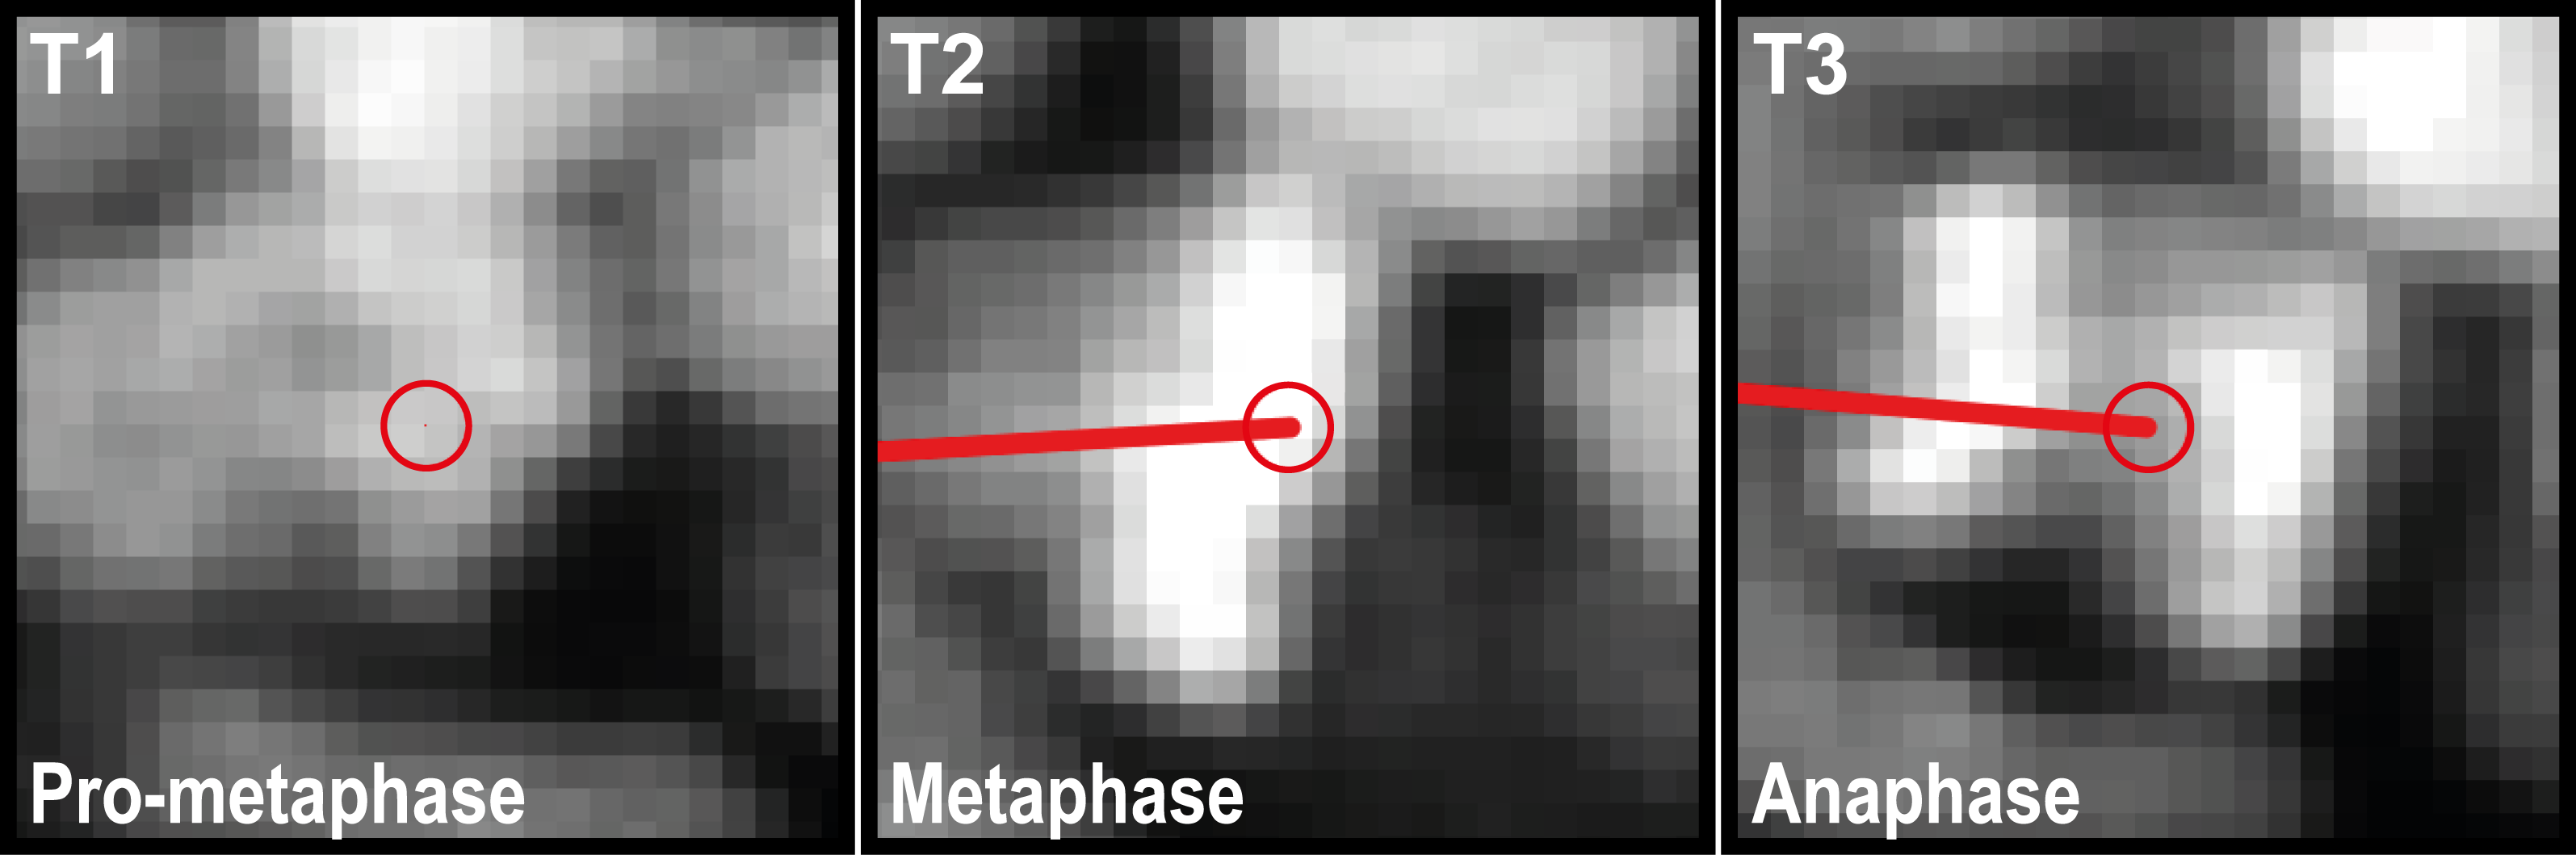
\includegraphics[width=0.6\linewidth]{figures/materials/prol/Prolif} 

}

\caption[Tracking of mitotic events]{Tracking of mitotic events. T1-T3 show consequetive timepoints of a single nucleus.}\label{fig:mitodatapoints}
\end{figure}
\hypertarget{ACI}{%
\subsubsection{Apical Index}\label{ACI}}

\hypertarget{rationale}{%
\paragraph{Rationale}\label{rationale}}

The earliest attempt found for indexing AC can be found in a study published by Lee \emph{et al}(\emph{60}) where they were interested in the `apical index' (A.I.) of bottle cells during \emph{X.laevis} gastrulation (figure \ref{fig:ACLee} Lee). Another example for measuring AC is the \emph{apical constriction index} (A.C.I., figure \ref{fig:ACLee} Harding) for the cells of the \emph{D.rerio} lateral line primordium (pLLP), which can be found in a study from 2012 where it was shown that FGFr-Ras-MAPK signaling is required for Rock2a localization and AC (\emph{61}, \emph{62}).


\begin{figure}[H]

{\centering 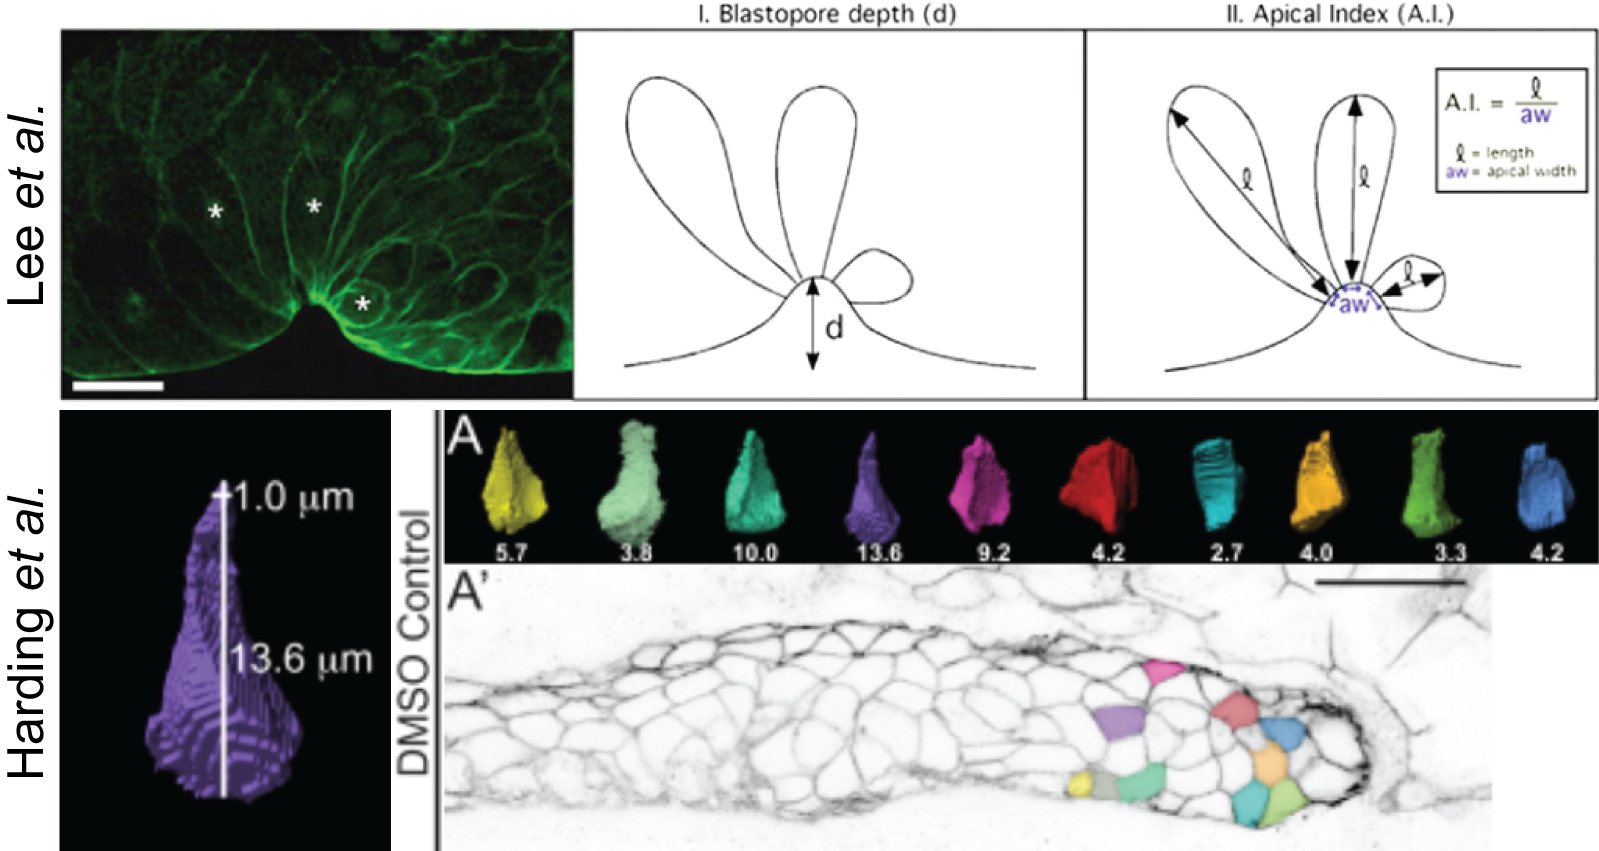
\includegraphics[width=0.75\linewidth]{figures/materials/models/ai} 

}

\caption[A.I. indeces in the literature]{A.I. indeces in the literature. \textbf{Lee} A.I. of \emph{X.leavis} bottle cells measured in 2D. \textbf{Harding} A.I. of \emph{D.r.} pLLP cells measured in 3D.}\label{fig:ACLee}
\end{figure}
\noindent In these two publications, the way they measure A.I. (\emph{60}) and ACI (\emph{62}) respectively, does not differ and is the ratio of lateral height over apical width.

\[\mathbf{ACI} = \frac{lateral\;height\;[\mu m]}{apical\;width\;[\mu m]}\]

\noindent We found two principal weaknesses of applying this ratio to the cells of the pLLP. First, it does not respect the independence of lateral height to AC. Second, it does not differentiate between constriction along the \emph{anterio-posterior} (AP) or the \emph{dorso-ventral} (DV) axis. Third, it actually represents the A.I. rather than the apical \emph{constriction} index.

\hypertarget{ACI-param}{%
\subparagraph{Parameter definition}\label{ACI-param}}

To obtain a precise and biologically meaningful way to quantify AC, first a couple of definitions had to be made.
\begin{definition}[AC is independent of orientation]
\protect\hypertarget{def:unnamed-chunk-3}{}{\label{def:unnamed-chunk-3} \iffalse (AC is independent of orientation) \fi{} }In a 3D space a cell can have any orientation and still be apically constricted. Therefore, before measuring one should make sure orientation between embryos is aligned and also consider taking measurements along two different directions. Since apical constriction is not necessarily isotropic, it is important to consider constriction along 2 perpendicular axes (AP and DV axis of the embryo/pLLP).
\end{definition}
\begin{definition}[AC is independent of lateral height]
\protect\hypertarget{def:unnamed-chunk-4}{}{\label{def:unnamed-chunk-4} \iffalse (AC is independent of lateral height) \fi{} }Lateral height can be described as the distance of the two farthest points on the surface area of a cell. Two cells with different lateral heights can be equally apically constricted.
\end{definition}
\begin{definition}[AC is independent of cell volume]
\protect\hypertarget{def:unnamed-chunk-5}{}{\label{def:unnamed-chunk-5} \iffalse (AC is independent of cell volume) \fi{} }The volume of a cell represents its size. A large cell can be equally constricted as a small cell.
\end{definition}
\hypertarget{ACI-lat}{%
\subparagraph{Adaption for variation in lateral height}\label{ACI-lat}}

To test different A.I. conditions, an apically constricted cell can be approximated by modeling a tetrahedron. For example, shrinking or enlarging a cell symmetrically should not affect the A.I.. As described by Harding(2014)(\emph{62}), the \emph{apical width} of a cell is measured first by manual 3-D reconstruction, second manual re-orientation, and third by going 1 \(\mu\)m from the apical tip into the cell (from now on referred to as \(\Delta\)ap, \ref{fig:ACICells}B). Finally, \emph{apical width} is the total width of the 2D object in the respective volume.

If \(\Delta\)ap is a constant, the A.I. in a symmetrically enlarged cell increases from e.g.~\textasciitilde15 to \textasciitilde23, since \emph{apical width} stays the same but lateral height increases (compare figure \ref{fig:ACICells}A to A'). On the contrary, if \(\Delta\)ap is adjusted relative to a cells lateral height, e.g.~by percentage, the A.I. in a symmetrically enlarged cell stays the same (compare figure \ref{fig:ACICells}A to A'').


\begin{figure}[H]

{\centering 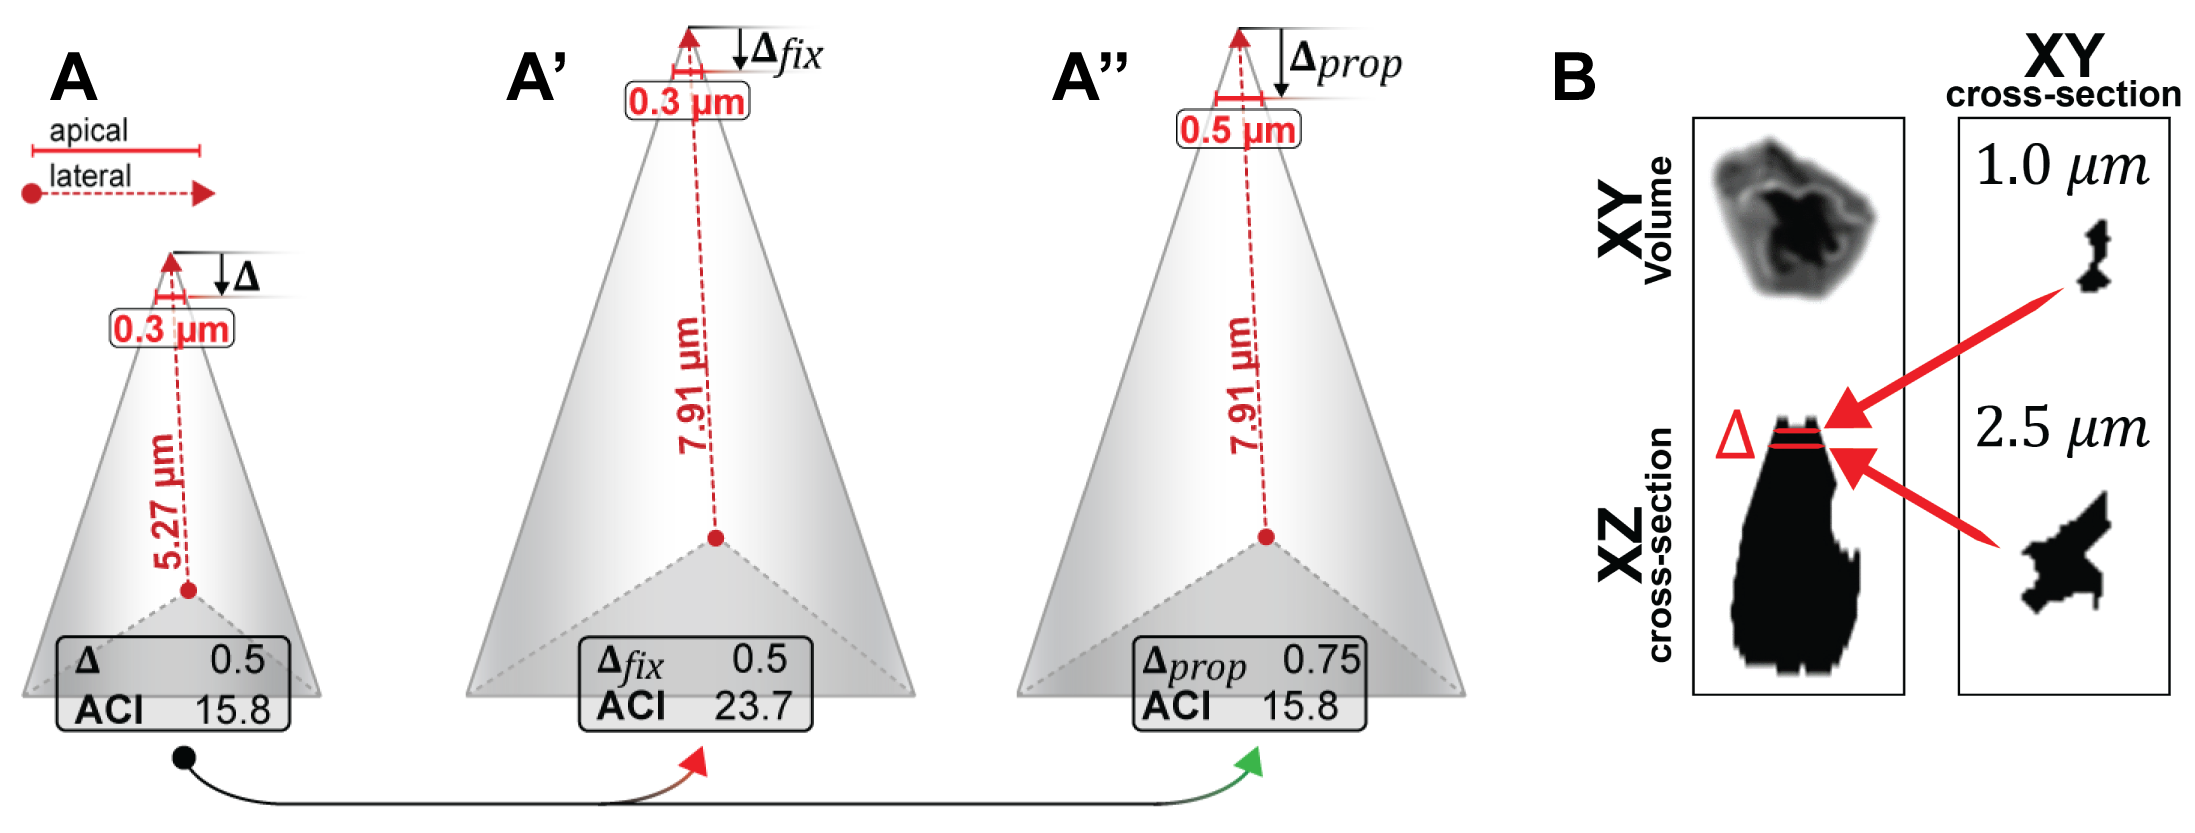
\includegraphics[width=0.85\linewidth]{figures/summary/aci_fig-01} 

}

\caption[Different ways to quantify the apical index]{Different ways to quantify the apical index. \textbf{A-A''} A.I. Cell Models. A' and A'' show cells that are symmetrically increased versions of A. While in A', constant delta was used, in A'' delta is proportional to the lateral height. \textbf{B} Illustrating delta ap. (left) apically constricted cells volume rendered in XY (top) and as a lateral cross-section in X-Z (bottom). (right) 2-D area as seen at \(\Delta\)ap of 1 or 2.5 \(\mu\)m.}\label{fig:ACICells}
\end{figure}
Therefore the measurement for apical width has to be relative to lateral height.

\[\mathbf{ACI} = \frac{lateral\;height\;[\mu m]}{relative\;apical\;width\;[\mu m]}\]

\hypertarget{ACI-pol}{%
\subparagraph{Adaption for tissue polarization}\label{ACI-pol}}

Organs develop in a 3-D space and are polarized along each axis. AC usually describes a 2-D morphogenetic movement towards a center along the X-Y axes. However, the constriction movements along X and Y might be independent of one another. This could mean that they happen at different speeds, or that one is absent. As a result, the tissue would look less radially (figure \ref{fig:cellpol}B) constricted, but more constricted along one particular axis (anisotropic). In order to separate those two AC dimensions, the A.I. can be calculated for the \emph{anterio-posterior} and for the \emph{dorso-ventral} axis (figure \ref{fig:cellpol}, horizontal vs.~vertical).


\begin{figure}[H]

{\centering 
\includegraphics[width=0.75\linewidth]{figures/materials/models/ACI_Cells_pol} 

}

\caption[Schematic anisotropic AC]{Schematic AC along the A-P and D-V axis. \textbf{A} shows a A-P and D-V constricted cluster of cells. \textbf{B} shows a D-V constricted cluster of cells.}\label{fig:cellpol}
\end{figure}
\noindent By fitting an ellipsoid to the area taken at \(\mathrm{\Delta}\)ap, one will obtain the following parameters (figure \ref{fig:ellipse}).
\begin{enumerate}
\def\labelenumi{\arabic{enumi}.}
\tightlist
\item
  Length of Major axis
  \begin{itemize}
  \tightlist
  \item
    indicates the level of constriction along the less constricted axis
  \end{itemize}
\item
  Length of Minor axis
  \begin{itemize}
  \tightlist
  \item
    indicates the level of constriction along the most constricted axis
  \end{itemize}
\item
  Angle of Major from 0\(^\circ\)
  \begin{itemize}
  \tightlist
  \item
    indicates the orientation of the long, less-constricted axis: If the angle is close to 0\(^\circ\), the long axis of the apical area is parallel to the AP axis (the cell is constricted along the DV axis). If the angle is close to 90\(^\circ\), the long axis of the apical area is parallel to the DV axis (the cell is constricted along the AP axis).
  \end{itemize}
\end{enumerate}

\begin{figure}[H]

{\centering 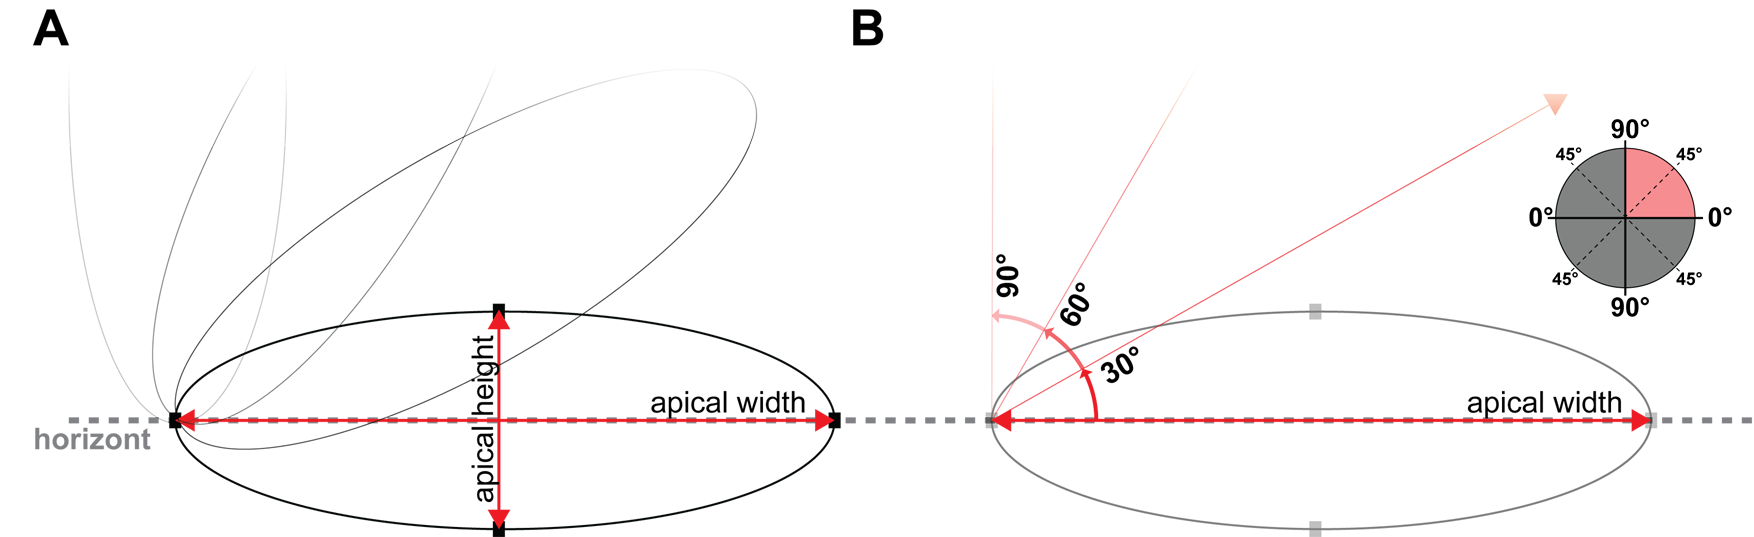
\includegraphics[width=0.75\linewidth]{figures/materials/models/ellipse} 

}

\caption[Scheme of ellipsoid measures]{Scheme of ellipsoid measures. \textbf{A} shows the major axis as apical width and the minor axis as apical height. \textbf{B} shows the angular displacement from the horizon in steps of 30\(^\circ\).}\label{fig:ellipse}
\end{figure}
\hypertarget{aci-theorem}{%
\subparagraph{Measurement definition}\label{aci-theorem}}

The two dimensions of A.I. indices can therefore be defined as the following ratios\ldots{}
\begin{definition}[A.I. Major]
\protect\hypertarget{def:unnamed-chunk-6}{}{\label{def:unnamed-chunk-6} \iffalse (A.I. Major) \fi{} }\[\mathbf{A.I._{Major}} = \frac{lateral\;height\;[\mu m]}{ellipsoid\;major\;axis\;at\;relative\;\Delta ap\;[\mu m]}\]
\end{definition}
\begin{definition}[A.I. Minor]
\protect\hypertarget{def:unnamed-chunk-7}{}{\label{def:unnamed-chunk-7} \iffalse (A.I. Minor) \fi{} }\[\mathbf{A.I._{Minor}} = \frac{lateral\;height\;[\mu m]}{ellipsoid\;minor\;axis\;at\;relative\;\Delta ap\;[\mu m]}\]
\end{definition}
\begin{definition}[Angle Major]
\protect\hypertarget{def:unnamed-chunk-8}{}{\label{def:unnamed-chunk-8} \iffalse (Angle Major) \fi{} }\[\mathbf{Angle_{Major}} = \measuredangle = \mathrm{\Delta}\;from\;horizon\;[0-90^\circ]\]
\end{definition}
\hypertarget{ACI-Dis}{%
\paragraph{Measurements}\label{ACI-Dis}}

As a proof of principle of the definitions stated in the previous section we compare our results to previously published results from Harding \emph{et al.} (\emph{61}) who, as a control, measured apical constriction in embryos treated with an FGF inhibitor (SU5402) and their DMSO controls.

\hypertarget{ACI-singlecell}{%
\subparagraph{Single Cell measurements}\label{ACI-singlecell}}

Each geometric object has a centroid coordinate in X and Y (and Z) which is represented as the mean of all X or Y coordinates within the object. In figure \ref{fig:ACICells}, centroid coordinates in X and Y are used to plot the cells as points in the X-Y plane. Additionally, each point is colored for the A.I. value (high values are dark red - red, middle values are green, low values are cyan - blue).


\begin{figure}[H]

{\centering 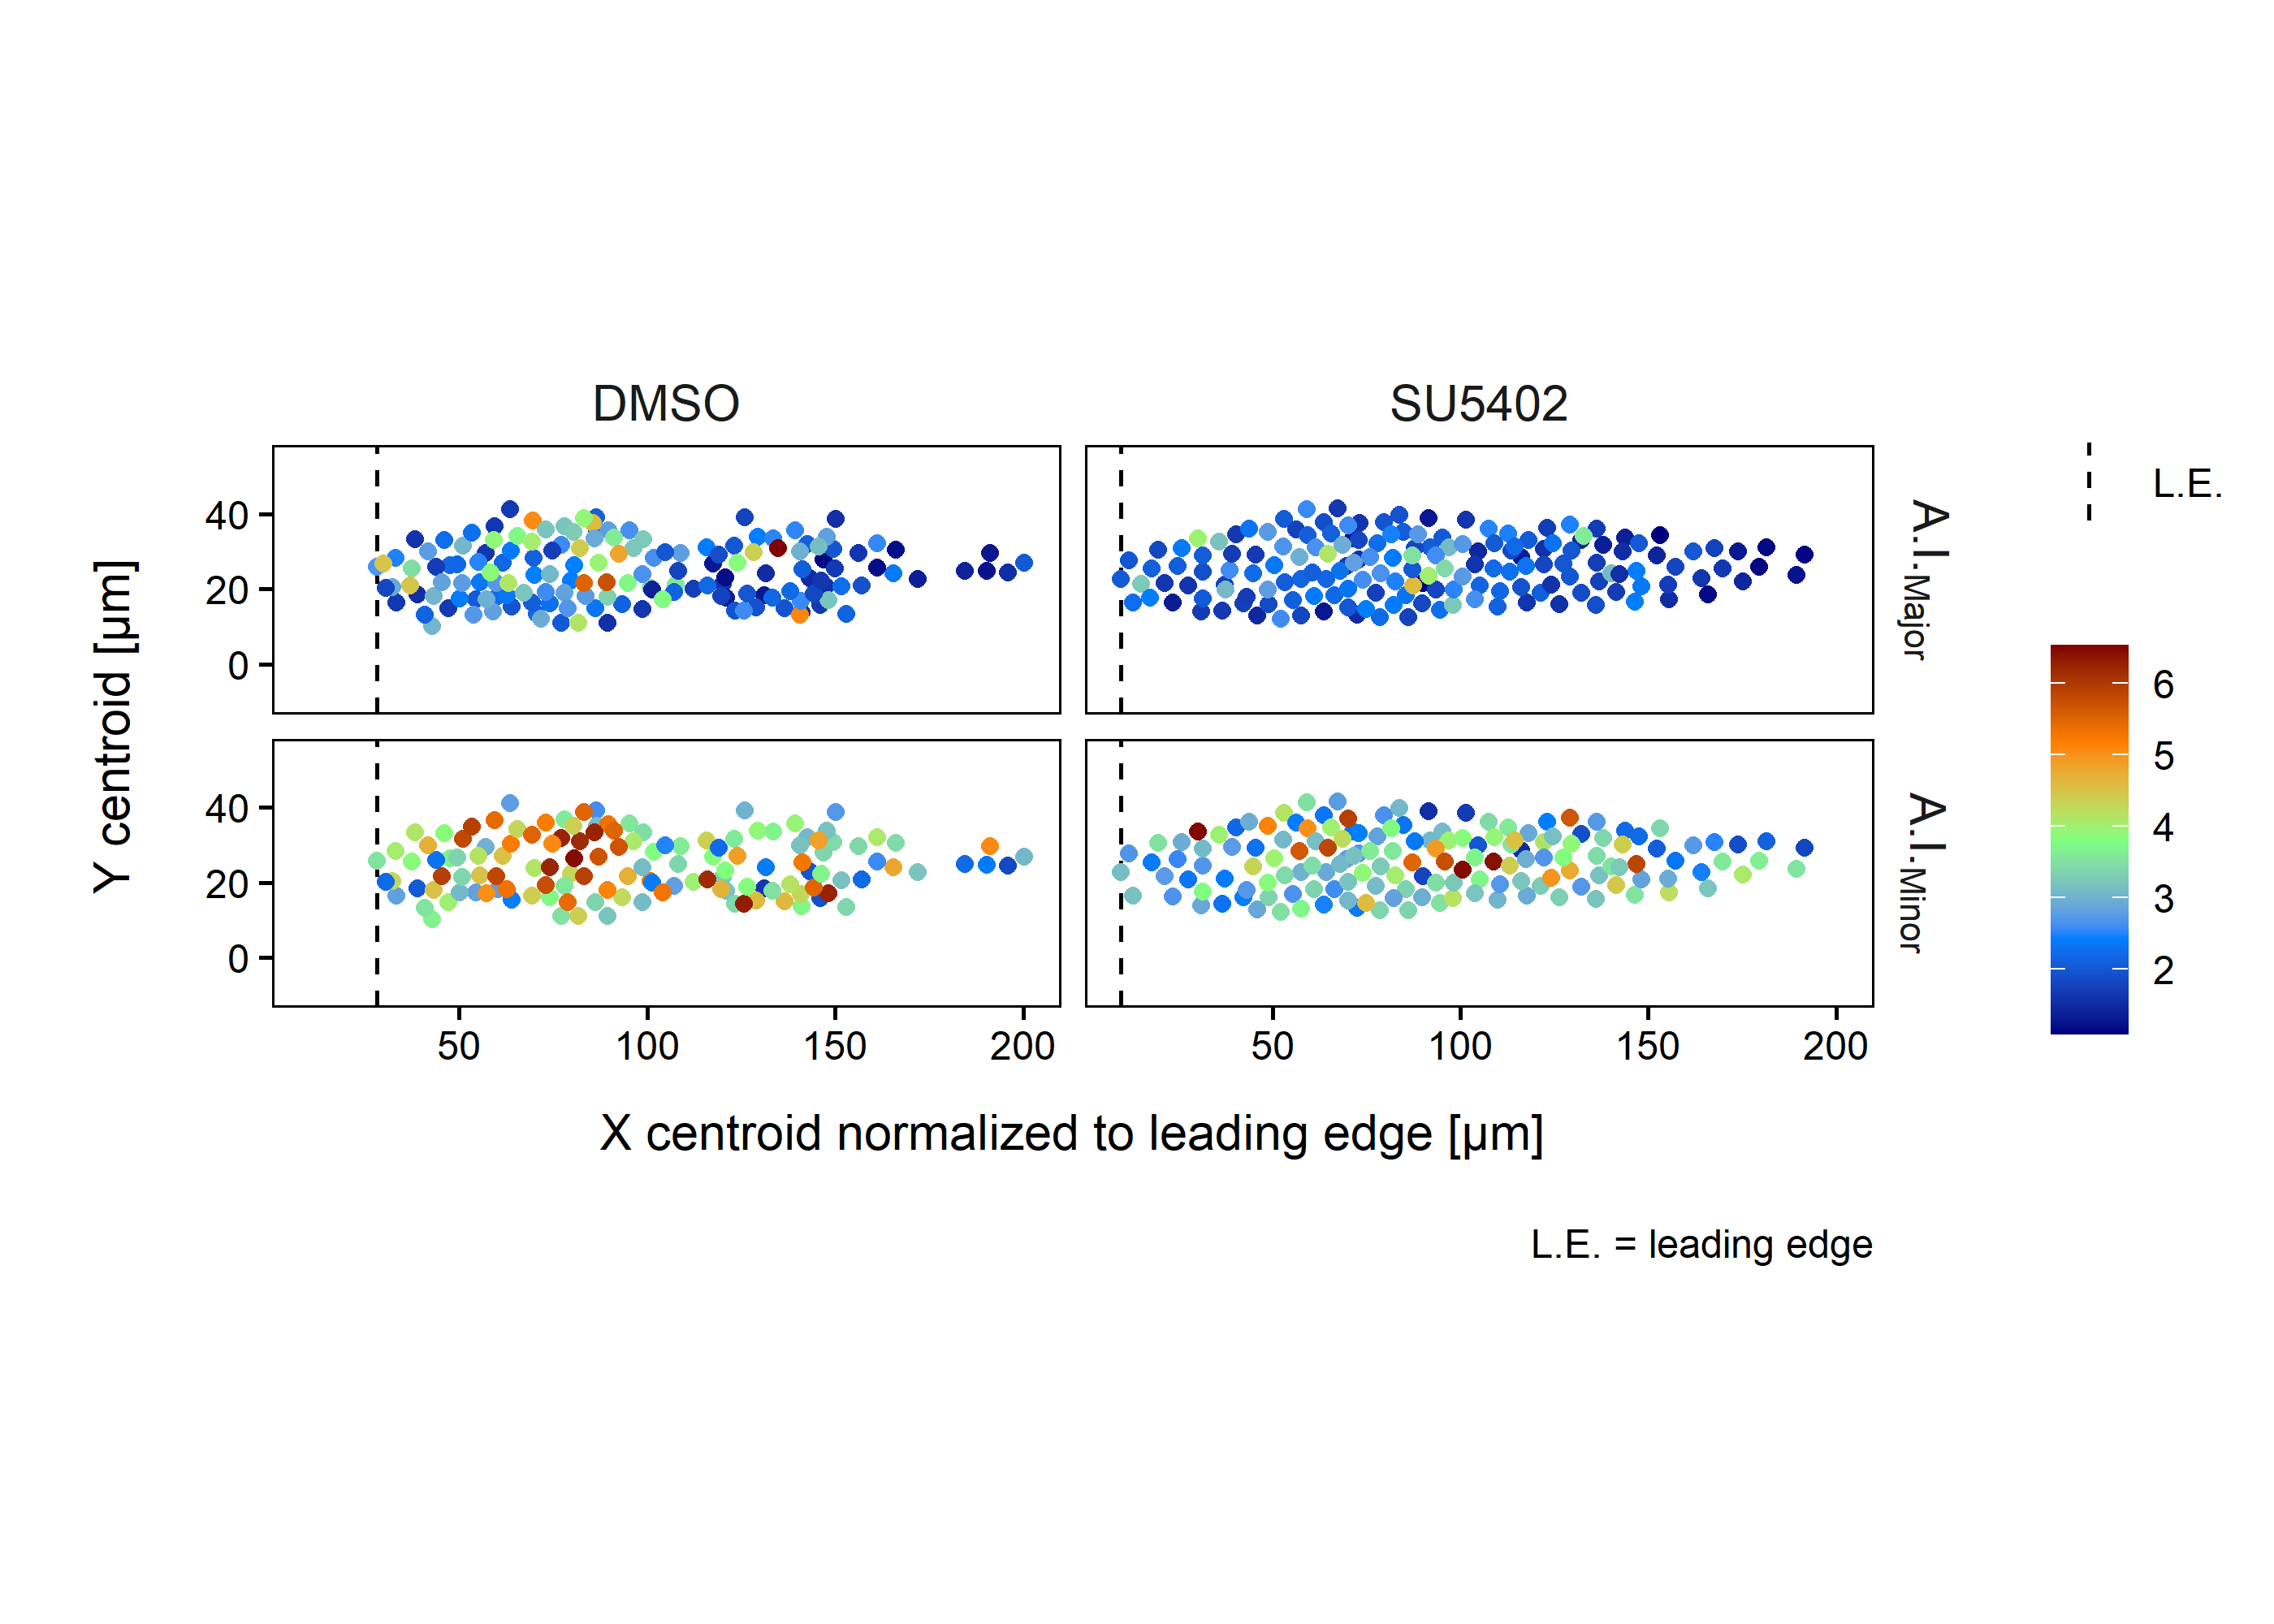
\includegraphics[width=0.95\linewidth]{thesis_dsk_files/figure-latex/aci-single-cell-measures-graph-1} 

}

\caption{A.I.\textsubscript{Major / Minor} single cell measurements}\label{fig:aci-single-cell-measures-graph}
\end{figure}
Harding \emph{et al.} (\emph{62}) were using a constant \(\mathrm{\Delta}\)ap to measure the apical width, which we have shown to be incorrect in certain cases. In their study they found that certain mean A.C.I. values in the DMSO go as high as 15 (figure \ref{fig:HardingACI}), which might be related to this (see figure \ref{fig:ACICells}). By measuring apical width at a relative \(\mathrm{\Delta}\)ap and taking into account all pLLP cells of the two exemplary pLLPs shown in figure \ref{fig:ACICells}, we measure a mean difference in the Major of 0.53 and 1.11 in the Minor.


\begin{figure}[H]

{\centering 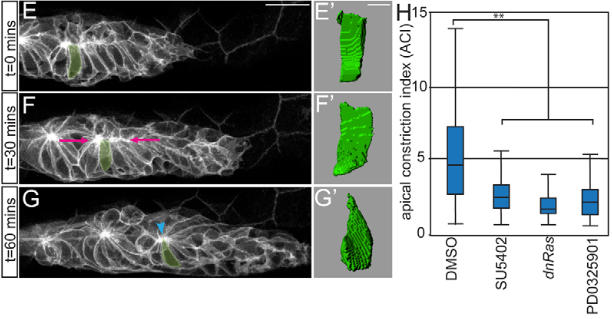
\includegraphics[width=0.6\linewidth]{figures/materials/models/harding} 

}

\caption[A.I. indices by Harding et al.]{A.I. indices by Harding et al.~\textbf{E-G'} 3-D reconstructions of the highlighted cell. \textbf{H} A.C.I.s for embryos treated with DMSO, SU5402, PD0325901 or following induction of \emph{hsp70:dn-Ras}. (n = 180 cells / N = 6 embryos).}\label{fig:HardingACI}
\end{figure}
\hypertarget{ACI-Angledens}{%
\subparagraph{Angle densities}\label{ACI-Angledens}}

To check whether there is a bias in orientation of the apical width, the angle measurements \ref{fig:ellipse} can be shown as a function of density along X (figure \ref{fig:angletoACI}A).

Interestingly the results indicate that there is less of a difference for the Major\textsubscript{Angle} at angles bigger than 15-20\(^\circ\). This would mean that the apical surface of the cells in SU5402 treated embryos is more strongly oriented along the horizontal \emph{antero-posterior} axis.

\hypertarget{ACI-mag}{%
\subparagraph{ACI magnitude at different Angles}\label{ACI-mag}}

Now, to get an idea of the magnitude of constriction relative to the orientation of the cell (angle to the horizontal), the A.I.\textsubscript{Major/Minor} can be shown as a function of the Major\textsubscript{Angle} (figure \ref{fig:angletoACI}B-B').

\noindent Since AC is a 3-D morphogenetic process and since cells in a wild type pLLP are mostly radially organized, it does make sense to try to look at AC from more than just one perspective. Here we propose to separate the A.I. into an \emph{antero-posterior} and a \emph{dorso-ventral} dimension.
\begin{enumerate}
\def\labelenumi{\arabic{enumi}.}
\item
  While for the control (DMSO treated) embryo the distribution of the cells Major Angles seem to be mostly uniform, for the SU5402 treated embryo there is an accumulation of lower Major Angles. This means that cells in SU5402 treated embryos are more oriented along the horizontal (anterior - posterior) axis.
\item
  Interestingly there does not seem to be much of a difference in A.I.\textsubscript{Major} (figure \ref{fig:angletoACI}B), which can also be shown by the mean values which are at 2.6 for the DMSO control and at 2.1 for the SU5402 treated condition.
\item
  For the A.I.\textsubscript{Minor} (figure \ref{fig:angletoACI}B') the means are 4.7 for the DMSO control and 3.6 for SU5402. The base constriction for both, DMSO and SU5402 is at around 3.6, however there is a peak at around 40 - 60\(^\circ\) in the DMSO control where cells are most constricted having a maximum A.I. at 15.8. This indicates that for the Minor, cells in that range of angles are more constricted than cells oriented in different directions.
\end{enumerate}

\begin{figure}[H]

{\centering 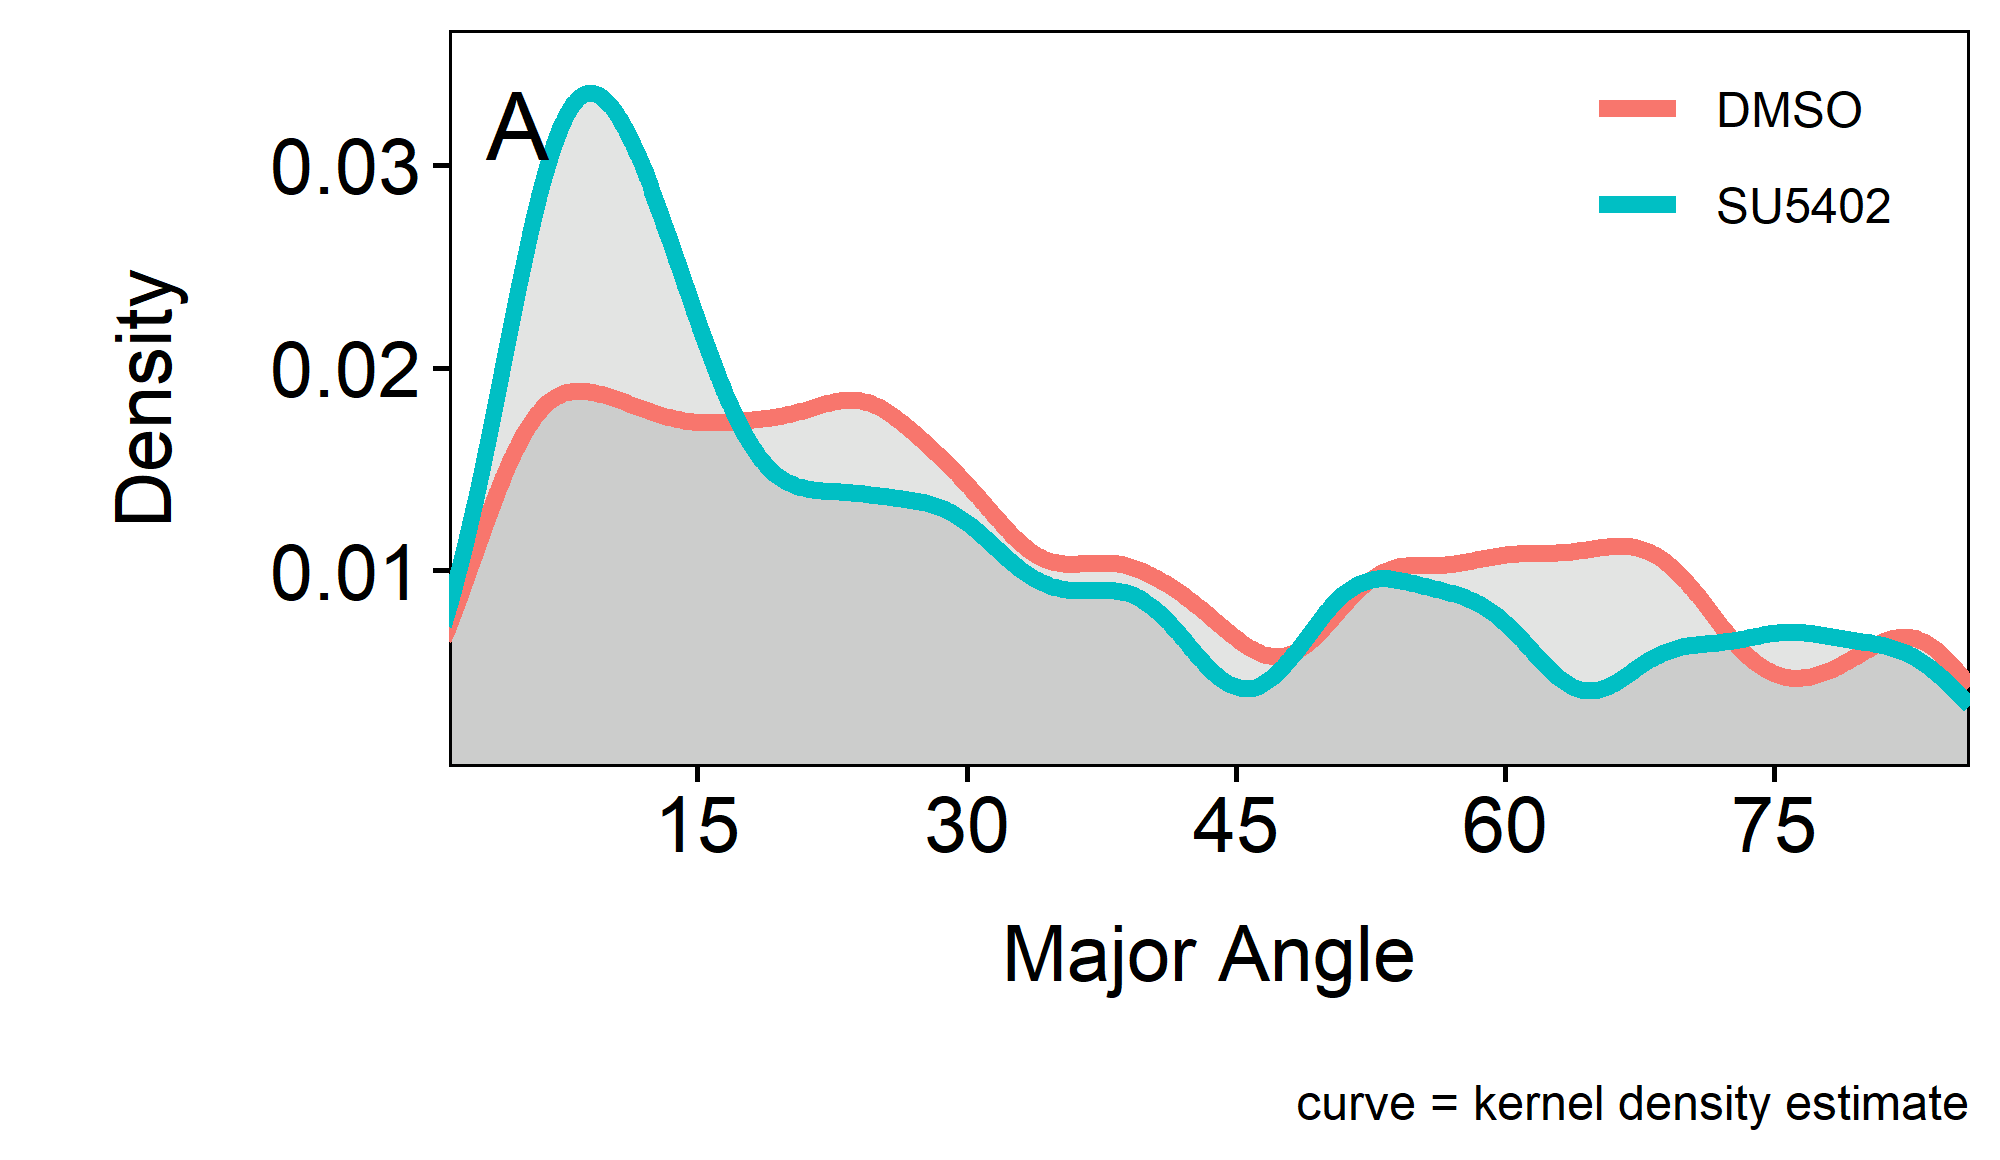
\includegraphics[width=0.49\linewidth]{thesis_dsk_files/figure-latex/angletoACI-1} 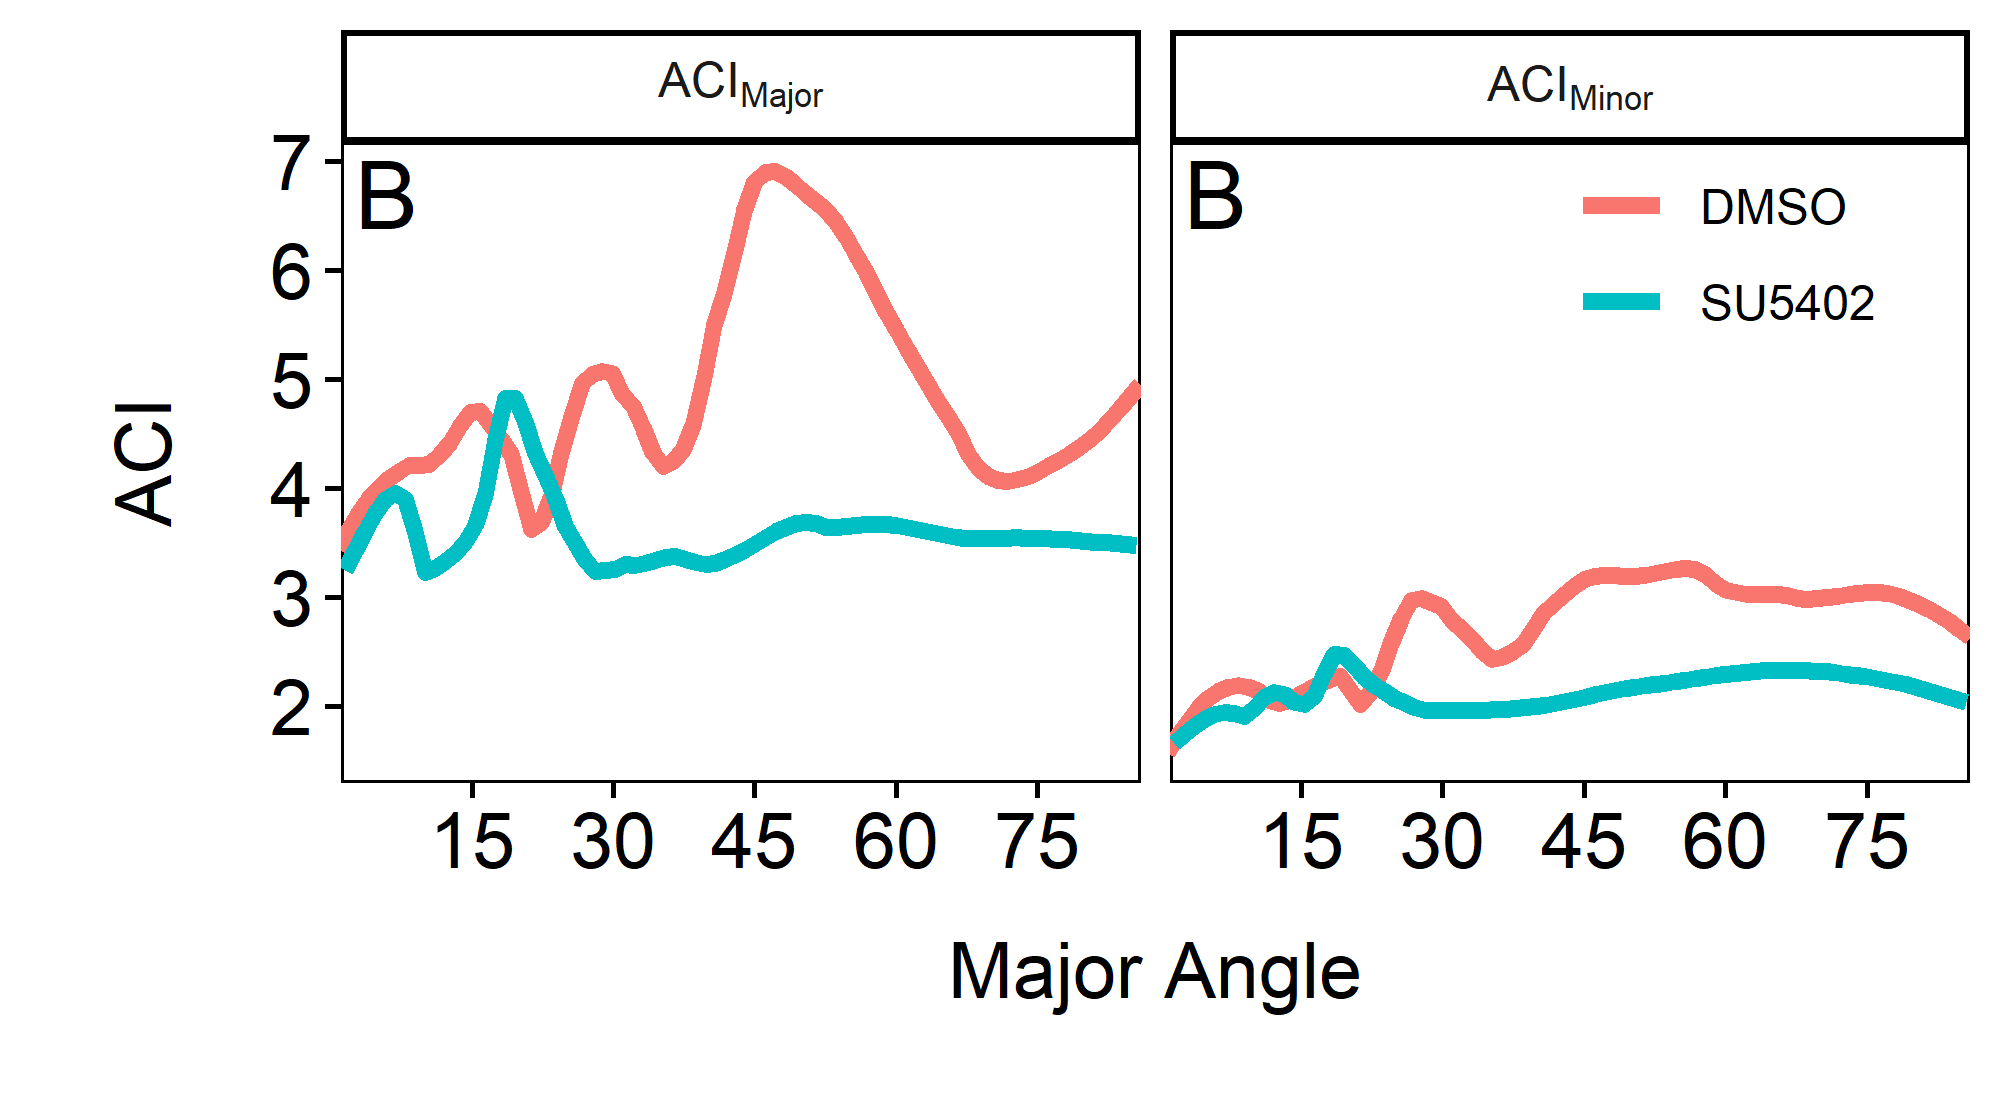
\includegraphics[width=0.49\linewidth]{thesis_dsk_files/figure-latex/angletoACI-2} 

}

\caption{A.I.\textsubscript{Major} / A.I.\textsubscript{Minor} over Major\textsubscript{Angle}}\label{fig:angletoACI}
\end{figure}
\hypertarget{mat-GrTrDat}{%
\section{Ground Truth}\label{mat-GrTrDat}}

Analyzing images and extracting quantitative measurements can be a tedious task, especially when the analysis becomes more complex. Fortunately, there are ways to automate image analysis by using either machine learning approaches or by tailoring hand-crafted algorithms in an image analysis software tool like e.g.~ImageJ(\emph{63}).
The main advantages of doing so are to\ldots{}
\begin{itemize}
\tightlist
\item
  be independent of confirmation bias
\item
  make the analysis more robust against oversight
\item
  increase the statistical power by increasing the number of data points(\emph{64})
\item
  increase effect size by increasing the measurement accuracy(\emph{64})
\end{itemize}
However, to ensure the measurements taken by a tailored or trained algorithm are meaningful, they must be compared to a \emph{ground truth} dataset which again describes a general measure of algorithmic quality performance(\emph{65}).

\hypertarget{cluster-analysis}{%
\subsection{Cluster Analysis}\label{cluster-analysis}}

The \emph{anaLLzR2D} algorithm was designed for semi-automatic cell cluster detection in the \emph{cldnb:lyn-gfp} transgenic line and optional nuclei counting in a second DAPI labeled channel within the Regions of Interest (ROIs) derived from the cell cluster detection.

\hypertarget{design}{%
\subsubsection{Design}\label{design}}

To assess the quality of the \emph{anaLLzR2D} algorithm for nuclei detection the ground truth was designed as follows.

\hypertarget{model}{%
\paragraph{Model}\label{model}}
\begin{itemize}
\tightlist
\item
  each Cell Cluster (CC) consists of a number of objects (cells)
\item
  each object is part of the respective CC and defines one cell entity
\item
  each object is determined via a fluorescent nucleus label
\item
  embryos are mounted within a 3D mold (section \ref{mount-met}) to reduce noise
\end{itemize}
\begin{longtable}[]{@{}rl@{}}
\caption{\label{tab:imgcond3DGrT} Cluster Analysis Model}\tabularnewline
\toprule
\endhead
\begin{minipage}[t]{0.46\columnwidth}\raggedleft
XY scale\strut
\end{minipage} & \begin{minipage}[t]{0.46\columnwidth}\raggedright
0.32 px/\(\mu\)m\strut
\end{minipage}\tabularnewline
\begin{minipage}[t]{0.46\columnwidth}\raggedleft
Z-spacing\strut
\end{minipage} & \begin{minipage}[t]{0.46\columnwidth}\raggedright
4 \(\mu\)m\strut
\end{minipage}\tabularnewline
\begin{minipage}[t]{0.46\columnwidth}\raggedleft
Camera\strut
\end{minipage} & \begin{minipage}[t]{0.46\columnwidth}\raggedright
Rolera\strut
\end{minipage}\tabularnewline
\bottomrule
\end{longtable}
\pagebreak

\hypertarget{training-test-data}{%
\paragraph{Training \& test data}\label{training-test-data}}

The training set consists of three randomly picked wild type pLLs. For each the algorithm was run with standard parameters. Cell cluster ROIs and nuclei multi-point labels were edited manually. To test the algorithm, it is run at different nuclei detection thresholds on the same image data.

\hypertarget{morphometric-analysis}{%
\subsection{Morphometric analysis}\label{morphometric-analysis}}

The \emph{anallzr3D} algorithm was designed for fully automated, single cell volume segmentation in the \emph{cldnb:lyn-gfp} transgenic line. In addition to 3D cellular metrics, it offers Apical Constriction measurement of each cell.

\hypertarget{design-1}{%
\subsubsection{Design}\label{design-1}}

To assess the quality of the anaLLzr3D algorithm the ground truth was modeled as follows.

\hypertarget{model-1}{%
\paragraph{Model}\label{model-1}}
\begin{itemize}
\tightlist
\item
  each pLLP consists of a number of objects (cells)
\item
  each object is part of the pLLP and defines one cell entity
\item
  cell boundaries are determined via the transgene \emph{cldnb:lyn-gfp} +/+
\item
  embryos are imaged live to conserve signal and membrane integrity
\item
  embryos are mounted within a 3D mold for improved 3D alignment
\end{itemize}
\begin{table}[!h]

\caption{\label{tab:model3DGrT}anaLLzr3D Model}
\centering
\begin{tabu} to \linewidth {>{\raggedleft\arraybackslash}p{4cm}>{\raggedright}X}
\toprule
\rowcolor{gray!6}  Exposure time & 100 ms\\
Laser intensity & 100$\%$ / 9.3 mW\\
\rowcolor{gray!6}  Objective & 40X; CFI APO LWD WI; N.A. = 1.15, W.D. = 0.60 mm\\
Tube lens & 1.0X\\
\rowcolor{gray!6}  Z-spacing & 0.4 - 0.5 $\mu$m\\
\addlinespace
Camera & sCMOS; 4.2 M.Pix; 82$\%$ Q.E.\\
\rowcolor{gray!6}  SD system & Yokogawa CSU - W1; 50 $\mu$m pattern\\
Piezo & Piezo Z-table; 300 $\mu$m scan range\\
\bottomrule
\end{tabu}
\end{table}
\hypertarget{training-test-data-1}{%
\paragraph{Training \& test data}\label{training-test-data-1}}

The training set consists of three randomly picked wildtype pLLPs. For each the algorithm is run with no filters (X, Y, Z border objects, size) and a minimum segmentation threshold. Afterwards the segmentation result is corrected manually for over- and under-segmentation and objects that are not part of the pLLP.

To test the algorithm it is run at different segmentation thresholds on the same image data.

\hypertarget{mat-datasets}{%
\section{Image Data Sets}\label{mat-datasets}}

Summaries of Image datasets. \emph{Pairs} describe the number of parent pairs I harvested eggs from. \emph{Stage} describes the time I waited for the parent pairs to mate and lay eggs. Since pair \#1 might have laid their eggs earlier than pair \#2, those batches would be some time apart in their \emph{staging}. \emph{Stamp} describes the version of the stamp I used, where the main difference between version 4 and 5 are more wells added and some minor upgrades in well-design.
\begin{table}[!h]

\caption{\label{tab:imgdatcc}Cell Cluster dataset}
\centering
\begin{tabu} to \linewidth {>{\raggedright\arraybackslash}p{2cm}>{\raggedright\arraybackslash}p{2.5cm}>{\raggedright}X}
\toprule
\rowcolor{gray!6}  Crossings & Pairs & 4\\
 & Transgenes & cldnb:lyn-gfp +/?\\

\rowcolor{gray!6}   & Mutation & shroom3\\

\multirow[t]{-3}{*}{\raggedright\arraybackslash Crossings} & Staging & 60 min.\\

\rowcolor{gray!6}   & Fixation & 4$\%$ PFA o.N.\\

\multirow[t]{-2}{*}{\raggedright\arraybackslash Mounting} & Agarose & 1$\%$ LMPA\\

\rowcolor{gray!6}   & Magnification & 25X WI + 1.0x zoom\\

 & Channels & 488 nm\\

\rowcolor{gray!6}  \multirow[t]{-3}{*}{\raggedright\arraybackslash Imaging} & Z-Stack & 2.5 $\mu$m Z-spacing; 110 $\mu$m stack size; 12*X large image\\
\bottomrule
\end{tabu}
\end{table}
\begin{table}[!h]

\caption{\label{tab:imgdatai}A.I. dataset}
\centering
\begin{tabu} to \linewidth {>{\raggedright\arraybackslash}p{2cm}>{\raggedright\arraybackslash}p{2.5cm}>{\raggedright}X}
\toprule
\rowcolor{gray!6}  Crossings & Pairs & 4\\
 & Transgenes & cldnb:lyn-gfp +/?\\

\rowcolor{gray!6}   & Mutation & shroom3\\

\multirow[t]{-3}{*}{\raggedright\arraybackslash Crossings} & Staging & 30 min.\\

\rowcolor{gray!6}   & Protocol & Kleinhans $\textit{et al.}$, 2019\\

 & Agarose & 0.5$\%$ LMPA + 20$\%$ Tricaine (V/V$\%$)\\

\rowcolor{gray!6}  \multirow[t]{-3}{*}{\raggedright\arraybackslash Mounting} & stamp & version 4A\\

 & Magnification & 40X objective + 1.0x zoom\\

\rowcolor{gray!6}   & Camera & Binning 1x1; Gain 1; Exposure 100 ms\\

 & Channels & 488 nm (100$\%$)\\

\rowcolor{gray!6}  \multirow[t]{-4}{*}{\raggedright\arraybackslash Imaging} & Z-Stack & 0.4 $\mu$m Z-spacing\\
\bottomrule
\end{tabu}
\end{table}
\begin{table}[!h]

\caption{\label{tab:imgdatprol}Proliferation dataset}
\centering
\begin{tabu} to \linewidth {>{\raggedright\arraybackslash}p{2cm}>{\raggedright\arraybackslash}p{2.5cm}>{\raggedright}X}
\toprule
\rowcolor{gray!6}  Crossings & Pairs & 6\\
 & Transgenes & cldnb:lyn-gfp +/?; cxcr4b(BAC):H2BRFP +/0\\

\rowcolor{gray!6}   & Mutation & shroom3\\

\multirow[t]{-3}{*}{\raggedright\arraybackslash Crossings} & Staging & 30 min.\\

\rowcolor{gray!6}   & Protocol & Kleinhans $\textit{et al.}$, 2019\\

 & Agarose & 0.3$\%$ LMPA + 20$\%$ Tricaine (V/V$\%$)\\

\rowcolor{gray!6}  \multirow[t]{-3}{*}{\raggedright\arraybackslash Mounting} & stamp & version 4A\\

 & Magnification & 20X + 1.5x zoom\\

\rowcolor{gray!6}   & Camera & Binning 2x2; Gain 4; Exposure 35 ms; full FOV*150 $\mu$m\\

 & Channels & 651 nm (25$\%$)\\

\rowcolor{gray!6}   & Z-Stack & 2.5 $\mu$m Z-spacing; 110 $\mu$m stack size; 2*X large image\\

\multirow[t]{-5}{*}{\raggedright\arraybackslash Imaging} & Time & 20 h / 7 min. interval / start ~ 2 p.m.\\
\bottomrule
\end{tabu}
\end{table}
\begin{table}[!h]

\caption{\label{tab:imgdatdet}Detection dataset}
\centering
\begin{tabu} to \linewidth {>{\raggedright\arraybackslash}p{2cm}>{\raggedright\arraybackslash}p{2.5cm}>{\raggedright}X}
\toprule
\rowcolor{gray!6}  Crossings & Pairs & 6\\
 & Transgenes & cldnb:lyn-gfp +/?\\

\rowcolor{gray!6}   & Mutation & shroom3\\

\multirow[t]{-3}{*}{\raggedright\arraybackslash Crossings} & Staging & 30 min.\\

\rowcolor{gray!6}   & Protocol & Kleinhans $\textit{et al.}$, 2019\\

 & Agarose & 0.3$\%$ LMPA + 20$\%$ Tricaine (V/V$\%$)\\

\rowcolor{gray!6}  \multirow[t]{-3}{*}{\raggedright\arraybackslash Mounting} & stamp & version 5A\\

 & Magnification & 20X + 1.5x zoom\\

\rowcolor{gray!6}   & Camera & Binning 2x2; Gain 4; Exposure 20 ms; full FOV*150 $\mu$m\\

 & Channels & 488 nm (25$\%$)\\

\rowcolor{gray!6}   & Positions & 36\\

 & Z-Stack & 3 $\mu$m Z-spacing; 100 $\mu$m stack size; 3*X large image\\

\rowcolor{gray!6}  \multirow[t]{-6}{*}{\raggedright\arraybackslash Imaging} & Time & 20 h / 10 min. interval / start ~ 2 p.m.\\
\bottomrule
\end{tabu}
\end{table}
\begin{table}[!h]

\caption{\label{tab:imgdatato}Atoh1a dataset}
\centering
\begin{tabu} to \linewidth {>{\raggedright\arraybackslash}p{2cm}>{\raggedright\arraybackslash}p{2.5cm}>{\raggedright}X}
\toprule
\rowcolor{gray!6}  Crossings & Pairs & 4\\
 & Transgenes & cldnb:lyn-gfp +/?; atoh1a:Tom +/0\\

\rowcolor{gray!6}   & Mutation & shroom3\\

\multirow[t]{-3}{*}{\raggedright\arraybackslash Crossings} & Staging & 30 min.\\

\rowcolor{gray!6}   & Protocol & Kleinhans $\textit{et al.}$, 2019\\

 & Agarose & 0.3$\%$ LMPA + 20$\%$ Tricaine (V/V$\%$)\\

\rowcolor{gray!6}  \multirow[t]{-3}{*}{\raggedright\arraybackslash Mounting} & stamp & version 5A\\

 & Magnification & 20X + 1.0x zoom\\

\rowcolor{gray!6}   & Camera & Binning 2x2; Gain 4; full FOV*150 $\mu$m\\

 & Channels & 488 nm (Int: 20$\%$; Exp: 25 ms)\\

\rowcolor{gray!6}   & Channels & 561 nm (Int: 30$\%$; Exp: 50 ms)\\

 & Positions & 36\\

\rowcolor{gray!6}   & Z-Stack & 2.5 $\mu$m Z-spacing; 100 $\mu$m stack size; 2*X large image\\

\multirow[t]{-7}{*}{\raggedright\arraybackslash Imaging} & Time & 20 h / 20 min. interval / start ~ 2 p.m.\\
\bottomrule
\end{tabu}
\end{table}
\hypertarget{res}{%
\chapter{Results}\label{res}}

\hypertarget{res-met}{%
\section{Quantitative imaging and image analysis}\label{res-met}}

\hypertarget{res-mount}{%
\subsection{A 3D-printed stamp to standardize sample mounting and semi-automatize imaging}\label{res-mount}}
\begin{tcolorbox}[colback = white, sharp corners = northwest]
\textbf{NOTE}
\tcblower
Most of Chapter 3.1.1 has been published as an article in the Journal BMC Biotechnology (Kleinhans and Lecaudey, BMC Biotechnology (2019) 19:68). The author contribution was described in the paper as follows: DSK designed the study, carried out the experiments and analysis of the results. VL provided the infrastructure and funding for performing the experiments. DSK and VL wrote the final manuscript. All authors read and approved the final manuscript. 
Some passages in this section 3.1.1 have been quoted \textit{verbatim} from the above-mentioned article for the scientific accuracy of the terms used.
\end{tcolorbox}
Even though on a macroscopic scale development is remarkably similar and synchronized process between zebrafish embryos, a single biological process on a \emph{microscopic} scale even in sibling embryos can look drastically different. Given the noisy and variable character of biological systems, it is important to record a sufficient number of samples to obtain a quantitative and representative view of a biological process. Furthermore, to process biological samples of whole organisms in a high-content manner it is important to have a standardized way of sample mounting, data acquisition, data processing and analysis.

However, imaging a high number of samples and generating large datasets to date is still largely limited by the classical way most scientists mount embryos for imaging. A number of factors limiting the standardization are summarized in table \ref{tab:resmountingtab}
\begin{table}

\caption{\label{tab:resmountingtab}Limitations of traditional zebrafish mounting techniques}
\centering
\fontsize{9}{11}\selectfont
\begin{tabu} to \linewidth {>{\raggedright}X>{\raggedright}X>{\raggedright}X>{\raggedright\arraybackslash}p{4.5cm}}
\toprule
\textbf{Standard Method} & \textbf{Limitations} & \textbf{Solutions} & \textbf{Improvement}\\
\midrule
\rowcolor{gray!6}  \begin{itemize}[leftmargin=0.6em, topsep=-0.5em, itemsep=0.2em]\item Mounting in 1$\%$ LMPA\end{itemize} & \begin{itemize}[leftmargin=0.6em, topsep=-0.5em, itemsep=0.2em]\item Polymerization speed limits the number of embryos that can be mounted in parallel\item Embryo growth is restricted by high-percentage LMPA\end{itemize} & \begin{itemize}[leftmargin=0.6em, topsep=-0.5em, itemsep=0.2em]\item Use lower concentration of LMPA\item Use heating device to keep the LMPA liquid longer\end{itemize} & \begin{itemize}[leftmargin=0.6em, topsep=-0.5em, itemsep=0.2em]\item Mounting time extended\item Growth and change in shape of the embryo allowed\item Sample size increased\item Embryo retrieval facilitated\item Possibility to grow embryos to adulthood afterwards\end{itemize}\\
\begin{itemize}[leftmargin=0.6em, topsep=-0.5em, itemsep=0.2em]\item No pre-defined positions\end{itemize} & \begin{itemize}[leftmargin=0.6em, topsep=-0.5em, itemsep=0.2em]\item Positioning and alignment in XY are neither standardized nor reproducible\end{itemize} & \begin{itemize}[leftmargin=0.6em, topsep=-0.5em, itemsep=0.2em]\item Mount embryos at pre-defined identically oriented and equidistant positions\end{itemize} & \begin{itemize}[leftmargin=0.6em, topsep=-0.5em, itemsep=0.2em]\item Relative positions of embryos identical in all experiments\item Easier setup of multi-dimensional imaging experiments\item Easier navigation between different XY locations\item Possibility for semi-automated imaging\item Identification of individual embryo facilitated for downstream experiments (genotyping)\end{itemize}\\
\rowcolor{gray!6}  \begin{itemize}[leftmargin=0.6em, topsep=-0.5em, itemsep=0.2em]\item No $\mu$-wells that model the average embryo shape at a defined developmental stage\end{itemize} & \begin{itemize}[leftmargin=0.6em, topsep=-0.5em, itemsep=0.2em]\item Time-consuming orientation of the embryos\item Body axes not aligned to optical sectioning in Z due to huge yolk sac\end{itemize} & \begin{itemize}[leftmargin=0.6em, topsep=-0.5em, itemsep=0.2em]\item Use $\mu$-wells that model the average embryo shape\end{itemize} & \begin{itemize}[leftmargin=0.6em, topsep=-0.5em, itemsep=0.2em]\item Orientation of individual embryos during mounting in LMPA much faster\item No need to re-orient the embryos in XY plane post-imaging\item Aligned morphological shapes in Z projections\item Reduced stack and file size\item Reduced photo-bleaching and toxicity- Reduced post-processing\item Increased scanning speed\item Improved signal-to-noise ratio\end{itemize}\\
\bottomrule
\end{tabu}
\end{table}
Therefore, especially for 3D segmentation and 2D tracking experiments where an exact staging and orientation of the embryo is necessary, there is a need for methods to standardize sample mounting and image acquisition of multiple embryos.

The protocol we describe here was designed to be used with XY scanning universal sample holders that usually come with any motorized-stage inverted microscope. Similar to previous approaches (\emph{66}--\emph{69}), it uses a 3D-printed stamping device to produce an Agarose imprint with a diameter of 20 mm on the cover glass of a 35 mm \(\mu\)-dish. The imprint consists of 44 equally spaced \(\mu\)-wells, which are designed to fit the average morphology of a zebrafish embryo between 24 and 96 hours-post-fertilization (hpf).

The aim was to develop a standardized mounting method allowing us to: (i) mount many samples in parallel in a 2D coordinate system of rows and columns, (ii) reduce the acquisition time and thus photo-bleaching and photo-toxicity during imaging, (iii) semi-automatize the acquisition, (iv) reduce the post-processing steps, and (v) facilitate subsequent processing such as genotyping due to a 1:1 correlation between image data and specimen arrangement sequence.

For mounting, an improved 3D specimen preparation and well-plate like sample navigation for zebrafish larvae confocal microscopy was developed with which lateral line development can be recorded over more than 20 h, in up to 44 positions, in a confocal Z-stack of less than 120 \(\mu\)m and a time interval of 5--10 min. (depending on the number of channels and exposure time). The stamp was designed to be used for embryos between 24 and 96 hpf. For a tailor-made well, embryos were fixed and imaged \emph{in toto} to measure the dimensions in X, Y and Z of different (whole embryo, trunk, yolk) embryonic structures (figure \ref{fig:mountmicro}B-B'). Using Microsoft 3D-Builder a well was assembled from basic shapes like cube, sphere and wedge. After, the well was duplicated a couple of times and put in a grid-like arrangement to fit on a disc base 20 mm in diameter. Printing was performed on a Formlabs extrusion printer (figure \ref{fig:mountmicro}C).


\begin{figure}

{\centering 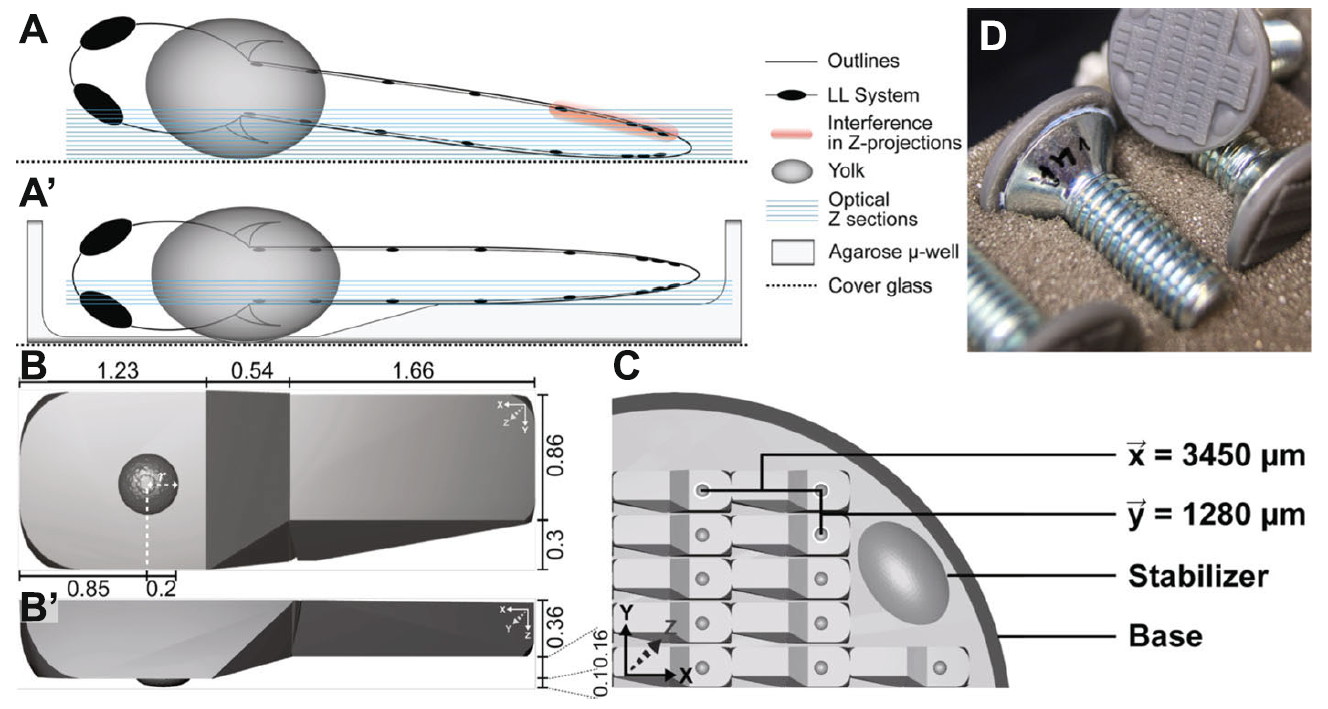
\includegraphics[width=0.95\linewidth]{figures/results/00_methods/mounting/stamp_dims} 

}

\caption[Stamp and micro-well properties]{Stamp and \(\mu\)-well properties. \textbf{A - A'} Mounting (A) without and with (A') \(\mu\)-well. Legend to the right. \textbf{B - B'} Dimensions of a single micro well in (B) X-Y and (B') X-Z in mm \textbf{C} Elements and dimensions of the stamp wafer. \emph{D} Assembled stamp with a screw mounted on the back of the stamp wafer.}\label{fig:mountmicro}
\end{figure}

\begin{figure}[H]

{\centering 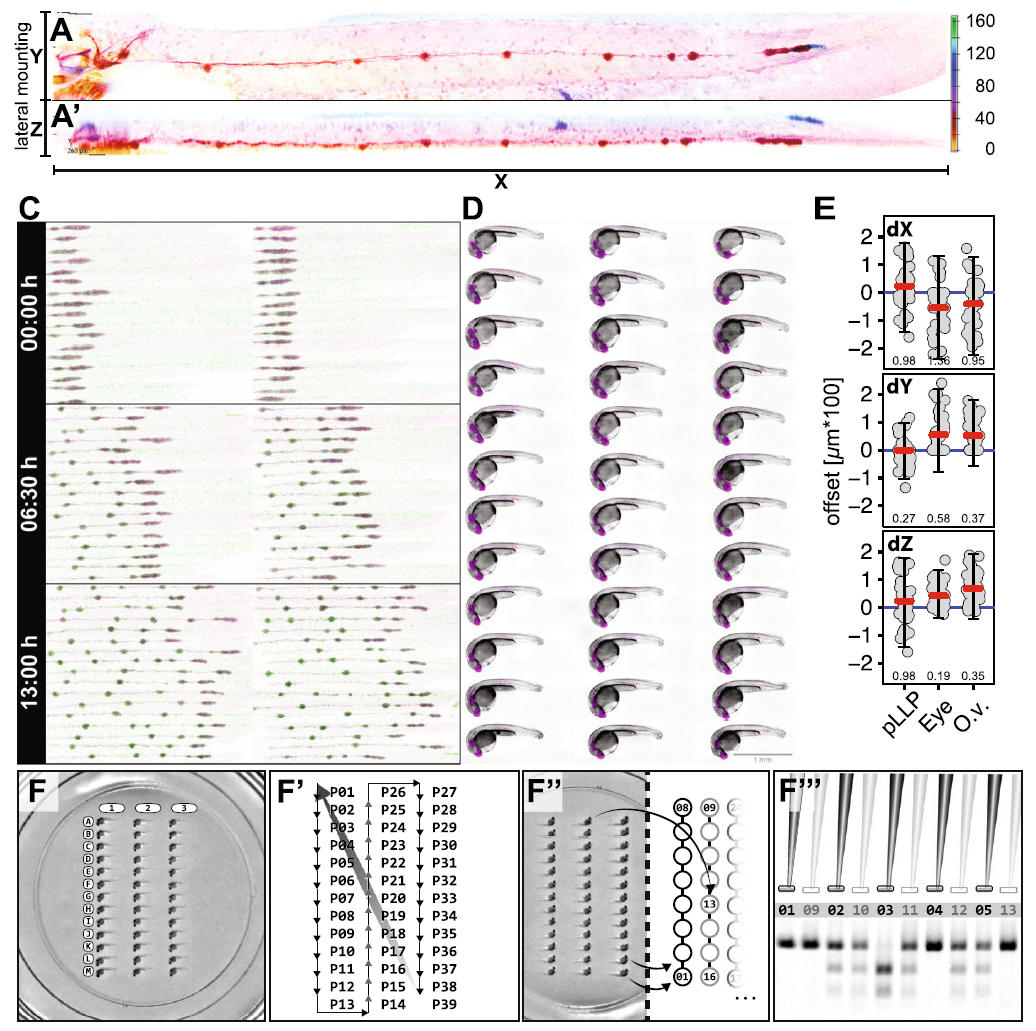
\includegraphics[width=0.95\linewidth,]{figures/results/00_methods/mounting/stamp_results} 

}

\caption[Mounting results]{Mounting Results. \textbf{A - A'} Maximum intensity projection of a 50 hpf embryo mounted on its side in XY and XZ. (right) Color scale indicates depth encoding. \textbf{C} Multi-position (36), multi-channel (2) time-lapse recording (13 h duration; 15 min. interval). \textbf{D} Multi-channel (2) Extended Depth of Focus (EDF) projections from widefield Z-stacks (recorded with 20x Objective). Scale Bar = 1mm \textbf{E} Multipoint coordinates in X, Y and Z (recorded with 40x Objective). The offset describes the distance of each point from the mean of all points in X, Y and Z. Panel 1--3 (top to bottom) show dimensions X, Y and Z in comparison for the pLLP, the eye and the otic vesicle. The red line indicates the median, the blue line indicates zero offset, error bars indicate mean \(\pm\) s.d.. Numeric values indicate the variance in each group. \textbf{F-F''} Systematic retrieval for genotyping. \textbf{F} Mounted embryos in a 2-D coordinate system of rows (A-M) and columns (1--3). \textbf{F'} Imaging Sequence in a snake-by-column fashion. In a time-lapse setting, it starts at point 1 (P01) again to initiate the next timepoint. \textbf{F''} After imaging, the embryos are retrieved in the same sequence as they were imaged (snake by column, left panel). \textbf{F''} Each genotyping result on the electrophoresis gel is easily correlated to one imaging dataset with defined X-Y coordinates.}\label{fig:stampresults}
\end{figure}
\hypertarget{procedure}{%
\subsubsection{Procedure}\label{procedure}}

\hypertarget{preparation-of-the-agarose-cast}{%
\paragraph{Preparation of the agarose cast}\label{preparation-of-the-agarose-cast}}

To prepare the agarose cast, the stamp is first cleaned from dust and remnants with tissue soaked in 70\(\%\) Ethanol and pressured air (figure \ref{fig:mounting} IA). To prepare the casting medium a 1\(\%\) Agarose (w/v) solution is prepared in an autoclaved 100 mL bluecap bottle by dissolving 200 mg of agarose in 20 mL of E3 using a microwave oven. From the ready solution 650 \(\mu\)L are applied to the \(\varnothing\) 20 mm coverslip of a \(\varnothing\) 35 mm imaging dish (materials in table \ref{tab:mat-mount}). Subsequently the clean stamp is gently placed onto the placed solution and adjusted to the center. The dish is then rotated to distribute excess agarose over the entire dish surface to stabilize the imprint once polymerized.

After about 30 min. the stamp is removed by first slipping a clean preparation needle between the stamp and the polymer and then lifting it from the cast (figure \ref{fig:mounting}IB). If necessary, air bubbled appearing between the cover glass and the polymer are eliminated by punctuation with a preparation needle. The mounting cast may be used immediately or stored at 4\(^\circ\)C for several days (with lid closed).

\hypertarget{preparation-of-mounting-media}{%
\paragraph{Preparation of mounting media}\label{preparation-of-mounting-media}}

Two solutions of low-melting point Agarose (LMPA) are prepared in autoclaved 100 mL bluecap bottles by dissolving 60 and 100 mg LMPA in 16 mL of E3 in a microwave oven - yielding 0.375 and 0.625 \(\%\) respectively. Per stamped cast, 2 aliquots of 1.6 mL are prepared in 2 mL tubes for each LMPA concentration and placed in a heating block adjusted to 41\(^\circ\)C.For live imaging, 400 \(\mu\)L of 4.2 mg/mL Tricaine (25X) are added to keep the embryos anesthetized during imaging. Final concentrations of LMPA solution are therefore 0.3 and 0.5 \(\%\), respectively. LMPA solutions containing Tricaine were prepared fresh for each mounting session. The LMPA solution and the mounting cast have almost equal refractive indices. Therefore, when adding the LMPA solution the cast becomes invisible. To still be able to locate the \(\mu\)-wells and to position the embryos accordingly, the illumination contrast and mirror angle of a transmitted light base are adjusted to make the \(\mu\)-wells visible again (figure \ref{fig:mounting}IIA-C).

\hypertarget{mounting-procedure}{%
\paragraph{Mounting procedure}\label{mounting-procedure}}

In case of live imaging the embryos are first anesthetized in a Petri dish with 4 to 5 drops of 4.2 mg/mL Tricaine (40 \(\mu\)g/mL in E3) added 4 to 5 min. before usage.

For mounting, the cast is first gently filled from the border (figure \ref{fig:mounting}II A3) with 500 \(\mu\)L of 0.3\(\%\) LMPA solution. Then, 44 embryos (one for each well) are collected from their Petri dish with a glass Pasteur pipette. To minimize the amount of liquid added to the LMPA, the embryos are allowed to sink to the air -- liquid interface and immediately added in one drop to the liquid LMPA solution in the stamped cast. Next, each embryo is moved to a separate \(\mu\)-well with a preparation needle by positioning the yolk within the half-spherical structure of each well and the tail aligned horizontally with the shape of the \(\mu\)-well (figure \ref{fig:mounting}II C-D). The LMPA was allowed to polymerize for about 40 min. For time-lapse recording longer than 1 h, 1 mL of 0.5\(\%\) LMPA was added on top and allowed to polymerize for another 10 min. to construct an Agarose \emph{sandwich} to stabilize the structure. Since the 0.3\(\%\) LMPA will still be very fragile, the 0.5\(\%\) LMPA should be added to the outer well first, carefully raising the level.

Since Agarose polymerization speed depends on temperature, for mounting the temperature of the room should not be less than 23\(^\circ\)C to give sufficient time. For indefinite time of embryo orientation, a higher room temperature or a 5 V terrarium heating mat (at maximum temperature ca. 38\(^\circ\)C) can be used. For the latter, a hole with the diameter of an imaging dish should first be cut in the middle of the heating mat. For mounting, the mat should then be placed and fixed on the stereo-microscope stage with the dish in the hole.

\hypertarget{imaging-setup}{%
\paragraph{Imaging setup}\label{imaging-setup}}

The dish is placed onto the sample holder of an inverted confocal spinning disc microscope so that the embryos are aligned to the Y axis of the microscope stage. The stage is then moved to place the embryo at Position 01 (P01, top-left position) right above the objective (figure \ref{fig:mounting}III A).

\hypertarget{define-embryo-positions}{%
\subparagraph{Define embryo positions}\label{define-embryo-positions}}

Since the embryos are mounted in a 3-D grid with well defined dimensions, all positions can be defined \emph{via} a pre-defined points list that is loaded into the microscope software. For our system we use the `Nikon Imaging Software' where we move the stage to P01, define a multi-point list with distance X / distance Y = 3450 / 1280 \(\mu\)m, bring P01 into focus and offset all points in Z. The list can also be saved for re-use in a future experiment. Alternatively one can also define a custom well plate and calibrate the stage.

\hypertarget{refine-positions}{%
\subparagraph{Refine Positions}\label{refine-positions}}

Even though the mounting method allows for a precise positioning, each embryos physiology is still a bit different resulting in differences between positions but same structures of up to 100 \(\mu\)m in X, Y and Z (figure \ref{fig:stampresults}E). Therefore, before starting an experiment each position needs to be refined.

\hypertarget{retrieval}{%
\paragraph{Retrieval}\label{retrieval}}

For further experiments such as genotyping, the embryos are retrieved from the agarose in the same sequence as they were imaged (figure \ref{fig:stampresults}F'). To do so, a glass pipette is inserted into the agarose and directed to the head region of an embryo. By applying a gentle underpressure the embryo is then sucked into the glass pipette.

To lyse the embryos and extract the genomic DNA, each embryo is placed in a single tube of an 8-tube PCR strip. Since 8-tube PCR strips are designed to work with multichannel pipettes, the genotyping PCR is performed and analysed by gel electrophoresis using an 8x-multichannel pipette. When using a 34-well comb, the pipette tips will reach every second well of the agarose gel. Filling the wells staggered (offset by 1), one can load 4 × 8 wells in one row (figure \ref{fig:stampresults}F'`). Since each embryo has a defined position, it is straightforward to associate each genotype to the corresponding image data (figure \ref{fig:stampresults}F' - F'''). Since a single mismatch would mess up the entire experiment by resulting in a frameshift of the one-to-one correspondence, this is a very important feature. The imaging dish can be reused several times. For cleaning, the agarose bed is removed from the dish using a small scoop or preparation needle and wiped gently with a lint-free tissue soaked in Ethanol.


\begin{figure}[H]

{\centering \includegraphics[width=0.95\linewidth,]{figures/results/00_methods/mounting/stamp_mounting} 

}

\caption[Stamping procedure]{Stamping procedure \textbf{Agarose Cast} (A) clean stamp surface (B) preparation of the stamp before lifting (C) ready-for-use agarose imprint. \textbf{Mounting} (A) without LMPA (B and C) with LMPA, while the latter shows the imprint with light coming from a different angle, making the chambers visible again. (D) Horizontal alignment of embryos. \textbf{Imaging} (A) Positioning of the \(\mu\)-well (B) Alignment in Brightfield and (C) Definition of a custom well plate.}\label{fig:mounting}
\end{figure}
\hypertarget{summary-1}{%
\subsubsection{Summary}\label{summary-1}}

The major improvements introduced by this method are (1) using a low percentage LMPA, which extends the timespan for mounting which is necessary to align a higher number of embryos. It also gives the embryo more freedom to grow during longer time-lapse imaging and facilitates retrieval of afterwards. (2) using a stamped cast, which allows for standardized and reproducible positions of the embryo as shown for the lateral line primordium, the eye and the otic vesicle (figure \ref{fig:stampresults}E). A significant increase of number of embryos that can be imaged during a single experiment (figure \ref{fig:stampresults}C-D). A significant reduction of the Z-stack size and therefore of the illumination of the samples (figure \ref{fig:stampresults}A).

In comparison to existing methods we provide a solution that is easy and in-expensive even for non-specialized labs. Also, while similar methods are well suited for high throughput and lower resolutions, ours may also be used for long time-lapse and high resolution imaging.

\hypertarget{mat-anallzr2d}{%
\subsection{anaLLzr2D - Automated 2D neuromast analysis and nuclei count}\label{mat-anallzr2d}}

For LL analysis I developed a custom IJ macro script that segments individual cell clusters and the pLLP. From the opening dialog (figure \ref{fig:anallzr2ddialog}) the user can choose to \emph{count nuclei} and / or \emph{sort ROIs}. If nuclei count is chosen, the macro expects a dual-channel (Ch1: \emph{cldnb:lyn-gfp}; Ch2: a nuclei label) \emph{tiff}-file as input. If ROI sorting is selected, segmented CCs are numbered and sorted from left to right instead of top to bottom (IJ's native sorting method).
\begin{itemize}
\tightlist
\item
  \emph{Membrane label blur} controls the detail of pLLP and CC segmentation, where lower values result in more detail
\item
  \emph{Closing filter} controls how harsh objects are separated from each other
\item
  \emph{Nuclei label blur} controls the details of single nuclei and is evaluated after ground truth data described in section \ref{mat-GrTrDat}
\end{itemize}

\begin{figure}[h]

{\centering 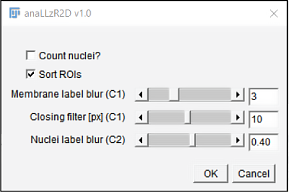
\includegraphics[width=0.4\linewidth,]{figures/materials/macros/anallzr2D_macro} 

}

\caption[anaLLzR2D opening dialog]{anaLLzR2D opening dialog \textbf{checkboxes} Choose to count nuclei and whether ROIs sorting should be applied. \textbf{sliders} Choose filter and blurring levels.}\label{fig:anallzr2ddialog}
\end{figure}
\hypertarget{image-analysis}{%
\subsubsection{Image Analysis}\label{image-analysis}}

Using ROIs as masks, the nuclei within each ROI are counted with a 2-D maxima finder. However, in their unprocessed form the images are too noisy to get meaningful results. The images therefore have to be smoothened with a blurring filter. To detect the right amount of nuclei, it is necessary to evaluate the distance over which the blurring should be applied. A typical nucleus in the pLLP is about 5 \(\mu\)m in diameter. To determine the right blurring value, a range of 4-6 \(\mu\)m in steps of 0.5 was tested. Figure \ref{fig:maxllreg} shows a registered maximum Z projected lateral line used for ground truth evaluation.


\begin{figure}[h]

{\centering 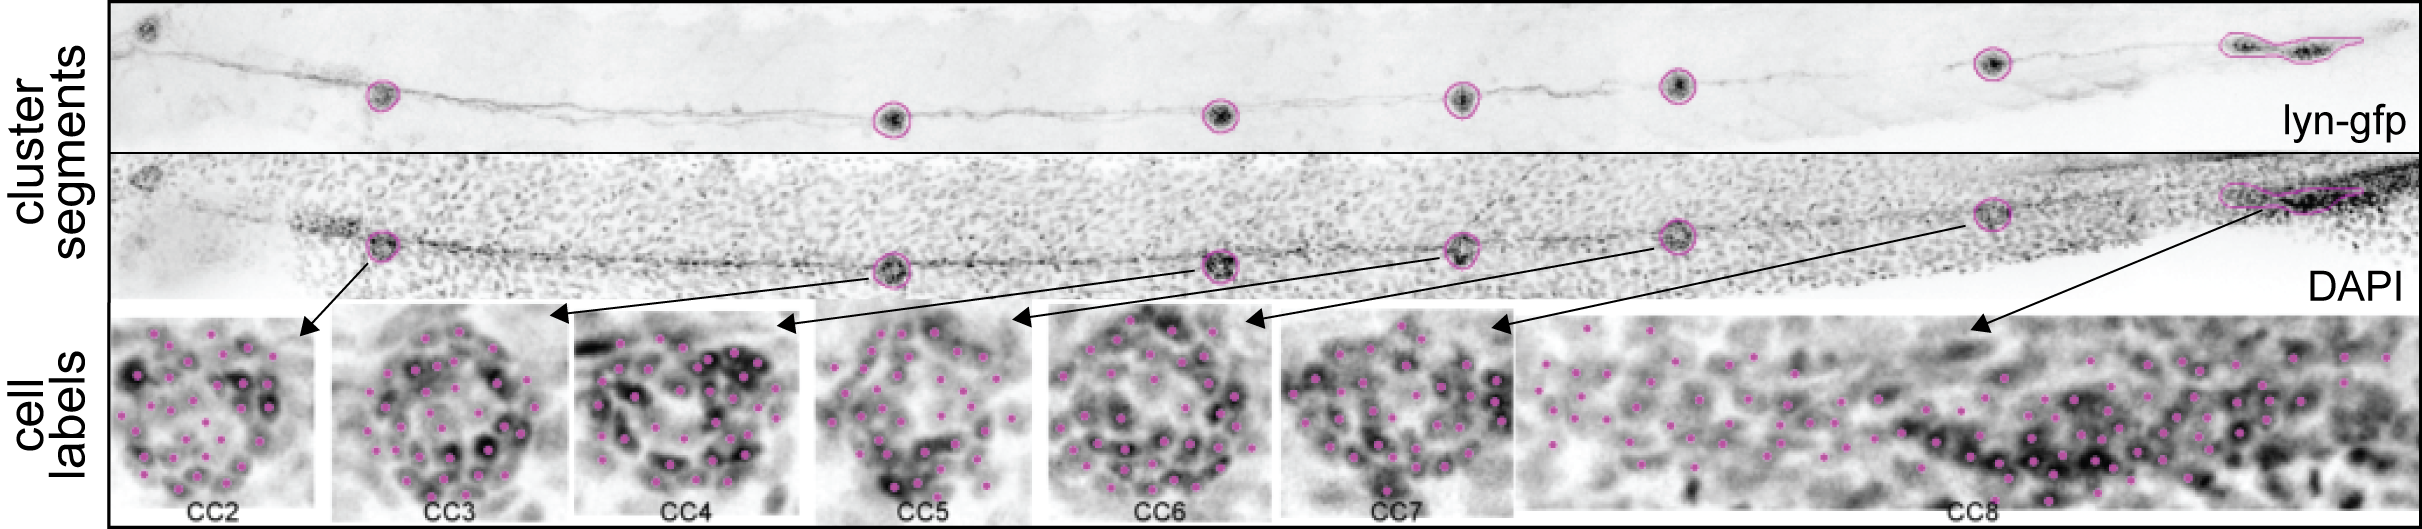
\includegraphics[width=0.95\linewidth,]{figures/materials/ground_truth/clusters/clusters} 

}

\caption[Registration of 2D data]{Registration of 2D data. \textbf{Cluster Segments} Registered, MaxIP data with cell cluster segments of the lyn-GFP signal laid upon the DAPI signal. \textbf{Cell Labels} Magenta dots represent the maxima found within each ROI and hence the nuclei labels.}\label{fig:maxllreg}
\end{figure}
\hypertarget{code-snippets}{%
\subsubsection{Code Snippets}\label{code-snippets}}

\hypertarget{segmentation}{%
\paragraph{Segmentation}\label{segmentation}}

The membrane label image is segmented based on optimized filter parameters that were derived from trial and error. After, the macro halts for manual correction.

\scriptsize
\begin{Shaded}
\begin{Highlighting}[numbers=left,,]
\CommentTok{# Background subtraction}
    \KeywordTok{run}\NormalTok{(}\StringTok{"Subtract Background..."}\NormalTok{, }\StringTok{"rolling = 50"}\NormalTok{);}
    \KeywordTok{run}\NormalTok{(}\StringTok{"Morphological Filters"}\NormalTok{,}
        \StringTok{"operation = Opening element = Disk radius = 20"}\NormalTok{);}
    \KeywordTok{run}\NormalTok{(}\StringTok{"Gaussian Blur..."}\NormalTok{, }\StringTok{"sigma = 5 scaled"}\NormalTok{);}

\CommentTok{# Thresholding}
    \KeywordTok{setAutoThreshold}\NormalTok{(}\StringTok{"Moments dark"}\NormalTok{);}
    \KeywordTok{setOption}\NormalTok{(}\StringTok{"BlackBackground"}\NormalTok{, false);}
    \KeywordTok{run}\NormalTok{(}\StringTok{"Convert to Mask"}\NormalTok{);}

\CommentTok{# Particle analysis}
    \KeywordTok{run}\NormalTok{(}\StringTok{"Analyze Particles..."}\NormalTok{, }\StringTok{"size = 250-Infinity exclude add"}\NormalTok{);}
    \KeywordTok{roiManager}\NormalTok{(}\StringTok{"Show All without labels"}\NormalTok{);}
    \KeywordTok{run}\NormalTok{(}\StringTok{"Enhance Contrast"}\NormalTok{, }\StringTok{"saturated = 0.35"}\NormalTok{);}
    \KeywordTok{waitForUser}\NormalTok{(}\StringTok{"Check ROIs, correct if necessary"}\NormalTok{);}
    \ControlFlowTok{if}\NormalTok{ (sort) \{}
        \KeywordTok{sortROIs}\NormalTok{();}
\NormalTok{    \}}
\end{Highlighting}
\end{Shaded}
\normalsize

\hypertarget{sorting}{%
\paragraph{Sorting}\label{sorting}}

To sort manually corrected ROIs from left to right, each ROIs position in calculated relatively to total image width.

\scriptsize
\begin{Shaded}
\begin{Highlighting}[numbers=left,,]
\CommentTok{# Sort ROIs from left to right}
\ControlFlowTok{function} \KeywordTok{sortROIs}\NormalTok{() \{}
    \KeywordTok{run}\NormalTok{(}\StringTok{"Set Measurements..."}\NormalTok{, }\StringTok{"centroid redirect = None decimal = 0"}\NormalTok{);}
            \ControlFlowTok{for}\NormalTok{ (}\DataTypeTok{j =} \DecValTok{0}\NormalTok{ ; j }\OperatorTok{<}\StringTok{ }\KeywordTok{roiManager}\NormalTok{(}\StringTok{"count"}\NormalTok{); j}\OperatorTok{++}\NormalTok{) \{}
                \KeywordTok{roiManager}\NormalTok{(}\StringTok{"select"}\NormalTok{, j);}
                \KeywordTok{roiManager}\NormalTok{(}\StringTok{"measure"}\NormalTok{);}
\NormalTok{                x =}\StringTok{ }\KeywordTok{getResult}\NormalTok{(}\StringTok{"X"}\NormalTok{, }\DecValTok{0}\NormalTok{);}
\NormalTok{                w =}\StringTok{ }\KeywordTok{getWidth}\NormalTok{();}
\NormalTok{                a =}\StringTok{ }\NormalTok{x}\OperatorTok{/}\NormalTok{w;}
                \KeywordTok{roiManager}\NormalTok{(}\StringTok{"rename"}\NormalTok{, a);}
                \KeywordTok{run}\NormalTok{(}\StringTok{"Clear Results"}\NormalTok{);}
\NormalTok{                \}}
        \KeywordTok{setBatchMode}\NormalTok{(false);}
        \KeywordTok{roiManager}\NormalTok{(}\StringTok{"sort"}\NormalTok{); }
            \ControlFlowTok{for}\NormalTok{ (}\DataTypeTok{j =} \DecValTok{0}\NormalTok{ ; j }\OperatorTok{<}\StringTok{ }\KeywordTok{roiManager}\NormalTok{(}\StringTok{"count"}\NormalTok{); j}\OperatorTok{++}\NormalTok{) \{}
                \KeywordTok{roiManager}\NormalTok{(}\StringTok{"select"}\NormalTok{, j);}
                \KeywordTok{roiManager}\NormalTok{(}\StringTok{"rename"}\NormalTok{, j);}
                \KeywordTok{run}\NormalTok{(}\StringTok{"Clear Results"}\NormalTok{);}
\NormalTok{                \}   }
            \ControlFlowTok{for}\NormalTok{ (}\DataTypeTok{j =} \DecValTok{0}\NormalTok{ ; j }\OperatorTok{<}\StringTok{ }\KeywordTok{roiManager}\NormalTok{(}\StringTok{"count"}\NormalTok{); j}\OperatorTok{++}\NormalTok{) \{}
                \KeywordTok{roiManager}\NormalTok{(}\StringTok{"select"}\NormalTok{, j);}
                \KeywordTok{roiManager}\NormalTok{(}\StringTok{"rename"}\NormalTok{, j}\OperatorTok{+}\DecValTok{1}\NormalTok{);}
                \KeywordTok{run}\NormalTok{(}\StringTok{"Clear Results"}\NormalTok{);}
\NormalTok{                \}}
\NormalTok{\}}
\end{Highlighting}
\end{Shaded}
\normalsize

\hypertarget{count-nuclei}{%
\paragraph{Count nuclei}\label{count-nuclei}}

After smoothing the nuclei signal in the DAPI labeled channel, maxima are detected only within each ROI.

\scriptsize
\begin{Shaded}
\begin{Highlighting}[numbers=left,,]
\CommentTok{# count nuclei within segmented cell clusters}
\CommentTok{# steps performed on DAPI channel}
\CommentTok{# count nuclei}
    \KeywordTok{run}\NormalTok{(}\StringTok{"Gaussian Blur..."}\NormalTok{, }\StringTok{"sigma = 0.6 scaled"}\NormalTok{);}
    \KeywordTok{roiManager}\NormalTok{(}\StringTok{"open"}\NormalTok{, datdir }\OperatorTok{+}\StringTok{ }\NormalTok{filename }\OperatorTok{+}\StringTok{ "_ROIset.zip"}\NormalTok{);}
\NormalTok{    rcount =}\StringTok{ }\KeywordTok{roiManager}\NormalTok{(}\StringTok{"count"}\NormalTok{);}

\CommentTok{# for each ROI}
    \ControlFlowTok{for}\NormalTok{ (}\DataTypeTok{j =} \DecValTok{0}\NormalTok{ ; j }\OperatorTok{<}\StringTok{ }\NormalTok{rcount; j}\OperatorTok{++}\NormalTok{) \{}
        \KeywordTok{roiManager}\NormalTok{(}\StringTok{"open"}\NormalTok{, datdir }\OperatorTok{+}\StringTok{ }\NormalTok{filename }\OperatorTok{+}\StringTok{ "_ROIset.zip"}\NormalTok{);}
        \KeywordTok{roiManager}\NormalTok{(}\StringTok{"select"}\NormalTok{, j);}
            \KeywordTok{run}\NormalTok{(}\StringTok{"Duplicate..."}\NormalTok{, }\StringTok{" "}\NormalTok{);}
            \KeywordTok{run}\NormalTok{(}\StringTok{"Enhance Contrast"}\NormalTok{, }\StringTok{"saturated = 0.35"}\NormalTok{);}
            \KeywordTok{run}\NormalTok{(}\StringTok{"Find Maxima..."}\NormalTok{, }\StringTok{"noise = 0 output = [Point Selection]"}\NormalTok{);}
            \KeywordTok{run}\NormalTok{(}\StringTok{"Capture Image"}\NormalTok{);}
        \KeywordTok{roiManager}\NormalTok{(}\StringTok{"select"}\NormalTok{, j);}
        \KeywordTok{run}\NormalTok{(}\StringTok{"Find Maxima..."}\NormalTok{, }\StringTok{"noise = 0 output = Count"}\NormalTok{);}
\NormalTok{        NC =}\StringTok{ }\KeywordTok{getResult}\NormalTok{(}\StringTok{"Count"}\NormalTok{);}
        \KeywordTok{setResult}\NormalTok{(}\StringTok{"Nuclei"}\NormalTok{, j, NC);}
        \KeywordTok{setResult}\NormalTok{(}\StringTok{"Pos"}\NormalTok{, j, j }\OperatorTok{+}\StringTok{ }\DecValTok{1}\NormalTok{);}
\NormalTok{    \}}
\end{Highlighting}
\end{Shaded}
\normalsize

\hypertarget{data-analysis}{%
\subsubsection{Data Analysis}\label{data-analysis}}

Comparing the maxima counts of each Gaussian parameter with the Ground Truth gives an indication for false -positives resp. -negatives. In figure \ref{fig:GrTratioCC} the relative numbers for each blurring parameter can be seen in percentage above or below the mean cell count of the ground truth (blue horizon). The red area represents false negatives, the green false positives.


\begin{figure}[H]

{\centering 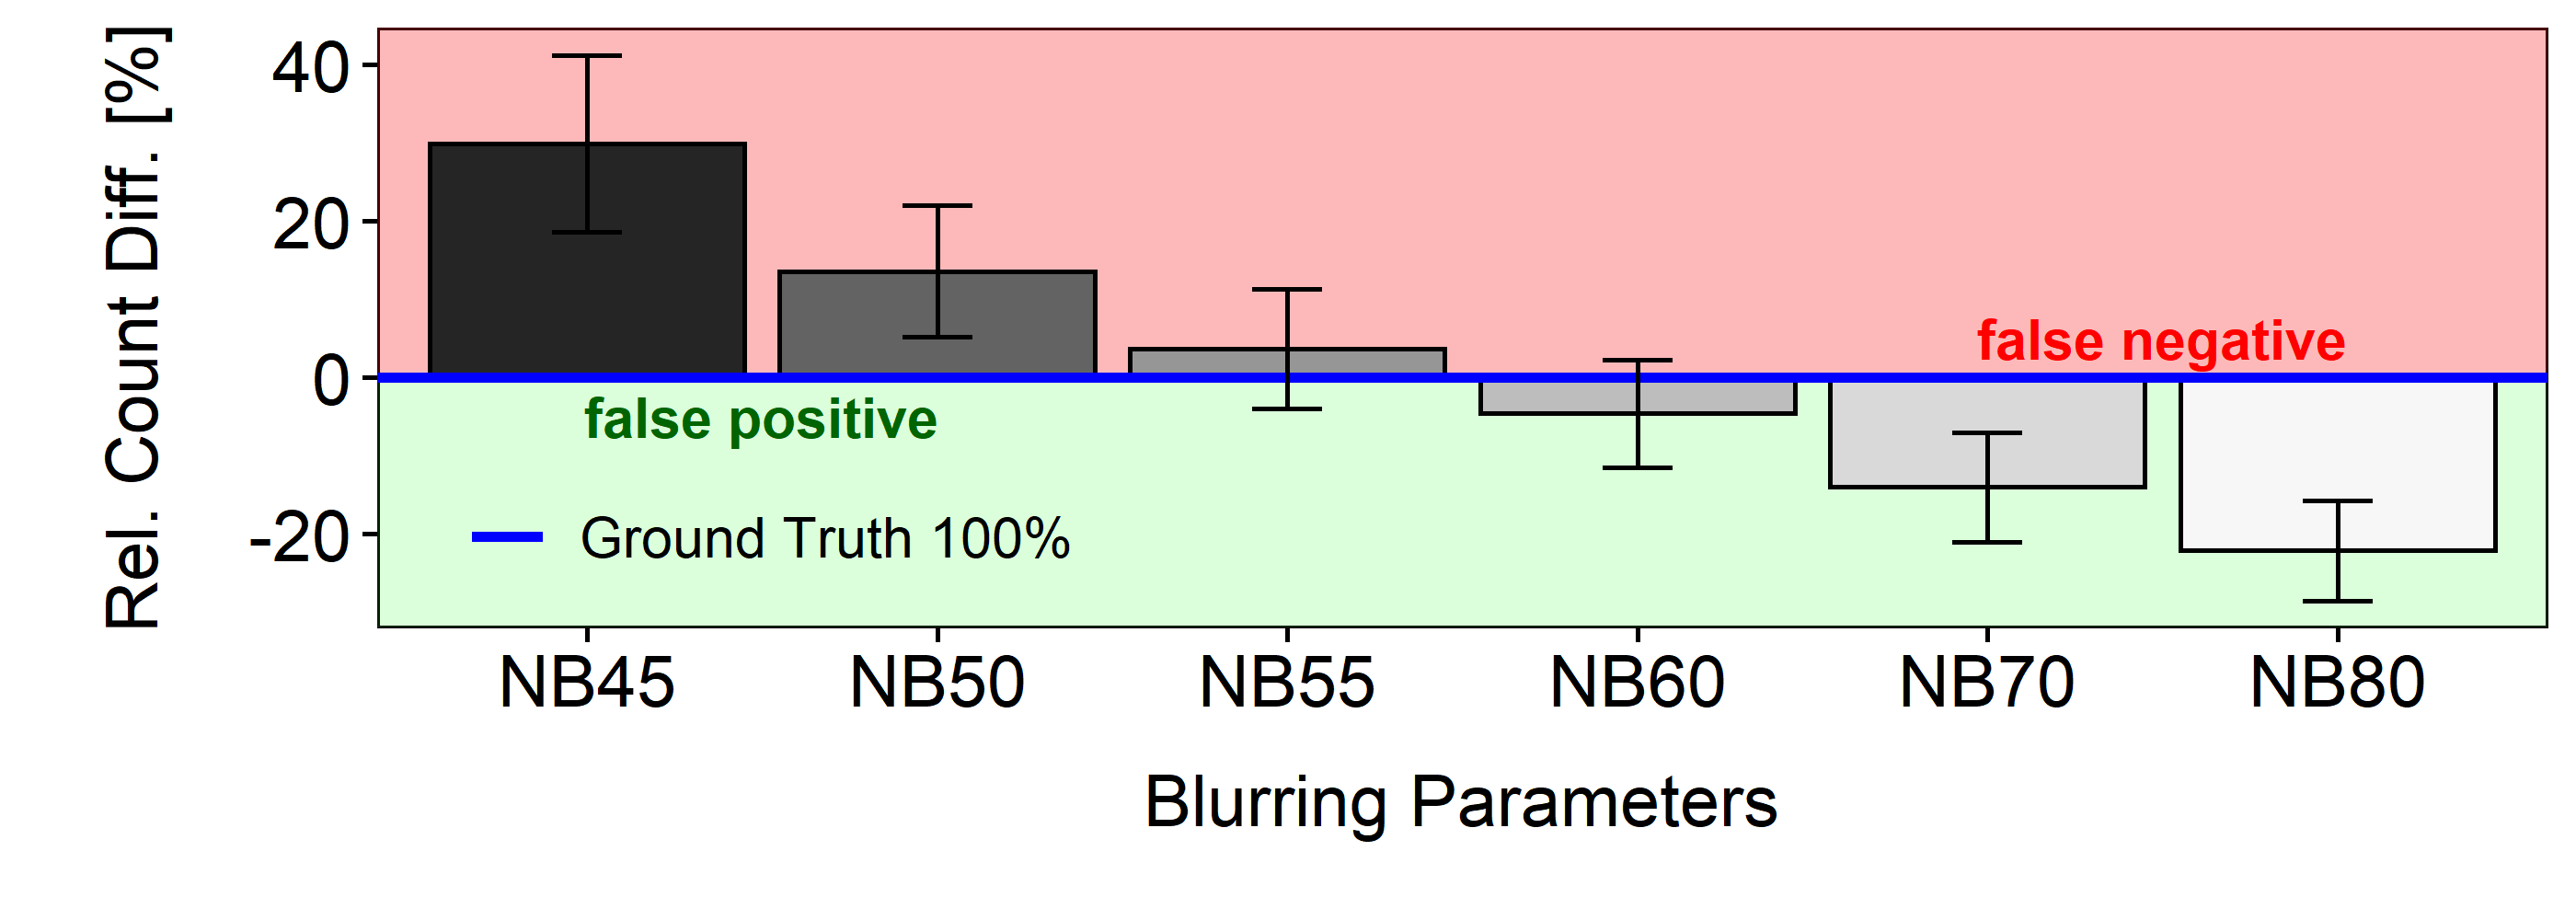
\includegraphics[width=0.65\linewidth]{thesis_dsk_files/figure-latex/GrTratioCC-1} 

}

\caption[Relative difference of maxima counts]{Relative difference of maxima counts}\label{fig:GrTratioCC}
\end{figure}
\noindent To estimate the quality of nuclei detection for each parameter, the ratio of automatically detected and ground truth objects count can be calculated and compared (table \ref{tab:nrcount}). The closer it is to 1, the better.
\begin{table}

\caption{\label{tab:nrcount}Blurring parameter for nuclei count}
\centering
\begin{tabu} to \linewidth {>{\raggedleft}X>{\centering}X>{\centering}X>{\centering}X>{\centering}X>{\centering}X}
\toprule
 & 4.5 & 5.0 & 5.5 & 6.0 & 7.0\\
\midrule
\rowcolor{gray!6}  mean ratio & 1.30 & 1.14 & 1.04 & 0.95 & 0.86\\
std. & 0.23 & 0.17 & 0.15 & 0.14 & 0.14\\
\bottomrule
\multicolumn{6}{l}{\textit{column headers}}\\
\multicolumn{6}{l}{blurring parameters}\\
\end{tabu}
\end{table}
In summary, maximum performance is achieved at a scaled parameter of 6 \(\mu\)m, with a ratio of of 0.95 for the count objects and a standard deviation of 0.14.

\hypertarget{mat-anallzr2dt}{%
\subsection{anaLLzr2DT - Automated 2D neuromast analysis and nuclei count through time}\label{mat-anallzr2dt}}

For the analysis of the migratory behavior (speed, acceleration) and shape (area, roundness) of the pLLP, as well as for the formation and deposition of the pro-Neuromasts through time, I developed a custom IJ macro script that segments the migrating pLLP and individual cell clusters on each frame of a timelapse. Upon macro execution the opening dialog is presented which is divided in three sections (figure \ref{fig:anallzr2dtdialog}A).

In the \textbf{processing} section the user may choose which modules are executed.
\begin{itemize}
\tightlist
\item
  \emph{Segmentation} controls whether the images are segmented before measurement. If de-seleted the user has to provide segmentation masks separately.
\item
  \emph{Include Cell Clusters} controls whether Cell Clusters should be included in the analysis. If de-selected, only the pLLP will be considered.
\item
  \emph{Registration} controls whether the pLLP should be captured in time and space and saved in a separate stack.
\item
  \emph{Multichannel} controls whether a second channel summary statistics from each ROI at each timepoint should be taken.
  \begin{itemize}
  \tightlist
  \item
    measurements taken are the mean, standard deviation, minimum and maximum intensity
  \end{itemize}
\end{itemize}
In the \textbf{options} section the user may choose whether the macro should be run in \emph{headless mode} (without showing every single action), whether the input images are timeseries and whether all other windows should be closed upon start of processing.

After confirmation, the user has to enter a date of experiment as an identifier in a second dialog. Furthermore the user is presented the images physical properties pre-filled where the idea here is just a review since this is a major source of mistakes (figure \ref{fig:anallzr2dtdialog}B). Finally, a third dialog is presented to the user giving an approximate duration and basic instructions (figure \ref{fig:anallzr2dtdialog}C).


\begin{figure}[H]

{\centering 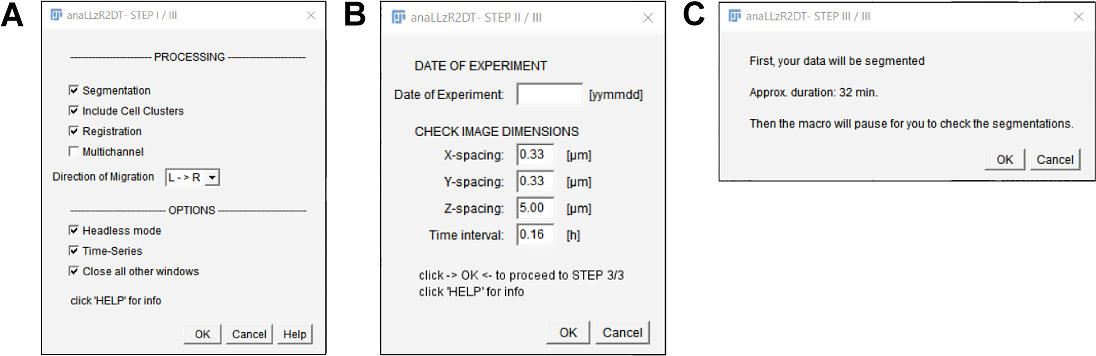
\includegraphics[width=0.95\linewidth]{figures/materials/macros/anallzr2DT_macro} 

}

\caption[anaLLzR2DT opening dialog]{anaLLzR2DT opening dialog \textbf{A} Opening dialog: Main functionality \textbf{B} Opening Dialog: metadata setup options \textbf{C} Time approximation dialog and basic instructions.}\label{fig:anallzr2dtdialog}
\end{figure}
Code-snippets describing the main functionality are described in the next couple of sub-sections.

\hypertarget{registration}{%
\subparagraph{Registration}\label{registration}}

The first module of the macro is pLLP registration in X, Y and cropping in Z. For better segmentation results, first the SNR is enhanced by background subtraction. To rotate the image the pLLPs migrational path is approximated by the position of the first and the last segment, then the image is cropped to a fixed height.

\scriptsize
\begin{Shaded}
\begin{Highlighting}[numbers=left,,]
\CommentTok{#   subtract background}
        \KeywordTok{run}\NormalTok{(}\StringTok{"Z Project..."}\NormalTok{, }\StringTok{"projection = [Average Intensity]"}\NormalTok{);}
\NormalTok{        ZPAVG =}\StringTok{ }\KeywordTok{getTitle}\NormalTok{();}
        \ControlFlowTok{if}\NormalTok{ (reg) \{}
            \KeywordTok{print}\NormalTok{(}\StringTok{"Calculating registration parameters..."}\NormalTok{);}
            \KeywordTok{setSlice}\NormalTok{(n);}
            \KeywordTok{run}\NormalTok{(}\StringTok{"Duplicate..."}\NormalTok{, }\StringTok{" "}\NormalTok{); }
\NormalTok{            DORG =}\StringTok{ }\KeywordTok{getTitle}\NormalTok{();}
            \KeywordTok{imageCalculator}\NormalTok{(}\StringTok{"Subtract create"}\NormalTok{, DORG, ZPAVG);}
            \KeywordTok{close}\NormalTok{(DORG);}
            \KeywordTok{run}\NormalTok{(}\StringTok{"Morphological Filters"}\NormalTok{,}
                \StringTok{"operation = Closing element=Disk radius = 15"}\NormalTok{);}
\NormalTok{            REG =}\StringTok{ }\KeywordTok{getTitle}\NormalTok{();}
            \KeywordTok{run}\NormalTok{(}\StringTok{"Gaussian Blur..."}\NormalTok{, }\StringTok{"sigma = 6 scaled"}\NormalTok{); }
            \KeywordTok{run}\NormalTok{(}\StringTok{"Duplicate..."}\NormalTok{, }\StringTok{" "}\NormalTok{);}
            \KeywordTok{run}\NormalTok{(}\StringTok{"Enhance Contrast..."}\NormalTok{, }\StringTok{"saturated = 0.3 normalize"}\NormalTok{);}
            \KeywordTok{run}\NormalTok{(}\StringTok{"8-bit"}\NormalTok{);}
            \KeywordTok{setAutoThreshold}\NormalTok{(}\StringTok{"MaxEntropy  dark"}\NormalTok{);}
            \KeywordTok{run}\NormalTok{(}\StringTok{"Convert to Mask"}\NormalTok{);}

    \CommentTok{# analyze segments}
        \KeywordTok{run}\NormalTok{(}\StringTok{"Analyze Particles..."}\NormalTok{, }\StringTok{"size = 150-10000 include exclude add"}\NormalTok{);}
\NormalTok{        rmcount =}\StringTok{ }\KeywordTok{roiManager}\NormalTok{(}\StringTok{"count"}\NormalTok{)}\OperatorTok{-}\DecValTok{1}\NormalTok{;}
        \KeywordTok{print}\NormalTok{(}\StringTok{"rois: "} \OperatorTok{+}\StringTok{ }\NormalTok{rmcount);}
        
    \CommentTok{# angle}
        \ControlFlowTok{if}\NormalTok{(}\KeywordTok{roiManager}\NormalTok{(}\StringTok{"count"}\NormalTok{) }\OperatorTok{==}\StringTok{ }\DecValTok{1}\NormalTok{) \{}
            \KeywordTok{roiManager}\NormalTok{(}\StringTok{"select"}\NormalTok{, }\DecValTok{0}\NormalTok{);}
\NormalTok{            List.setMeasurements;}
\NormalTok{            Angle =}\StringTok{ }\KeywordTok{List.getValue}\NormalTok{(}\StringTok{"FeretAngle"}\NormalTok{);}
            \KeywordTok{print}\NormalTok{(}\StringTok{"Angle: "} \OperatorTok{+}\StringTok{ }\NormalTok{Angle);}
            \ControlFlowTok{if}\NormalTok{ (Angle }\OperatorTok{<}\StringTok{ }\DecValTok{0}\NormalTok{) \{Angle =}\StringTok{ }\NormalTok{Angle }\OperatorTok{*}\StringTok{ }\NormalTok{(}\OperatorTok{-}\DecValTok{1}\NormalTok{);\}}
            \ControlFlowTok{if}\NormalTok{ (Angle }\OperatorTok{>}\StringTok{ }\DecValTok{90}\NormalTok{) \{Angle =}\StringTok{ }\NormalTok{(}\DecValTok{180}\OperatorTok{-}\NormalTok{Angle) }\OperatorTok{*}\StringTok{ }\NormalTok{(}\OperatorTok{-}\DecValTok{1}\NormalTok{);\}}
\NormalTok{        \} }\ControlFlowTok{else}\NormalTok{ \{}
            \KeywordTok{roiManager}\NormalTok{(}\StringTok{"select"}\NormalTok{, rmcount);}
\NormalTok{            List.setMeasurements;}
\NormalTok{            X1Line =}\StringTok{ }\KeywordTok{List.getValue}\NormalTok{(}\StringTok{"X"}\NormalTok{);}
\NormalTok{            Y1Line =}\StringTok{ }\KeywordTok{List.getValue}\NormalTok{(}\StringTok{"Y"}\NormalTok{);}
            \KeywordTok{roiManager}\NormalTok{(}\StringTok{"select"}\NormalTok{, }\DecValTok{0}\NormalTok{);}
\NormalTok{            List.setMeasurements;}
\NormalTok{            X2Line =}\StringTok{ }\KeywordTok{List.getValue}\NormalTok{(}\StringTok{"X"}\NormalTok{);}
\NormalTok{            Y2Line =}\StringTok{ }\KeywordTok{List.getValue}\NormalTok{(}\StringTok{"Y"}\NormalTok{);}
            \KeywordTok{makeLine}\NormalTok{(X1Line, Y1Line, X2Line, Y2Line);}
\NormalTok{            List.setMeasurements;}
\NormalTok{            Angle =}\StringTok{ }\KeywordTok{List.getValue}\NormalTok{(}\StringTok{"Angle"}\NormalTok{);}
            \ControlFlowTok{if}\NormalTok{ (Angle }\OperatorTok{<}\StringTok{ }\DecValTok{0}\NormalTok{) \{Angle =}\StringTok{ }\NormalTok{Angle}\OperatorTok{*}\NormalTok{(}\OperatorTok{-}\DecValTok{1}\NormalTok{);\}}
            \ControlFlowTok{if}\NormalTok{ (Angle }\OperatorTok{>}\StringTok{ }\DecValTok{90}\NormalTok{) \{Angle =}\StringTok{ }\NormalTok{(}\DecValTok{180}\OperatorTok{-}\NormalTok{Angle)}\OperatorTok{*}\NormalTok{(}\OperatorTok{-}\DecValTok{1}\NormalTok{);\}}
\NormalTok{            \}}
            \KeywordTok{print}\NormalTok{(}\StringTok{"Angle: "} \OperatorTok{+}\StringTok{ }\NormalTok{Angle);}
            \KeywordTok{run}\NormalTok{(}\StringTok{"Rotate... "}\NormalTok{, }
                \StringTok{"angle = "} \OperatorTok{+}\StringTok{ }\NormalTok{Angle }\OperatorTok{+}\StringTok{ " grid = 1 interpolation = Bilinear"}\NormalTok{);}
\NormalTok{            ZPAVG =}\StringTok{ }\KeywordTok{getTitle}\NormalTok{();}
            \KeywordTok{selectWindow}\NormalTok{(REG);}
            \KeywordTok{run}\NormalTok{(}\StringTok{"Rotate... "}\NormalTok{, }
                \StringTok{"angle = "}\OperatorTok{+}\StringTok{ }\NormalTok{Angle }\OperatorTok{+}\StringTok{" grid = 1 interpolation = Bilinear"}\NormalTok{);}
            \KeywordTok{run}\NormalTok{(}\StringTok{"Make Binary"}\NormalTok{);}
\NormalTok{            REG =}\StringTok{ }\KeywordTok{getTitle}\NormalTok{();}
        
        \CommentTok{# cropping}
            \KeywordTok{roiManager}\NormalTok{(}\StringTok{"reset"}\NormalTok{);}
            \KeywordTok{run}\NormalTok{(}\StringTok{"Analyze Particles..."}\NormalTok{, }
                \StringTok{"size = 150 - 10000 include add"}\NormalTok{);}
            \KeywordTok{roiManager}\NormalTok{(}\StringTok{"select"}\NormalTok{, }\DecValTok{0}\NormalTok{);}
\NormalTok{            List.setMeasurements;}
\NormalTok{            XRect =}\StringTok{ }\KeywordTok{List.getValue}\NormalTok{(}\StringTok{"X"}\NormalTok{);}
\NormalTok{            YRect =}\StringTok{ }\KeywordTok{List.getValue}\NormalTok{(}\StringTok{"Y"}\NormalTok{);}
            \KeywordTok{selectWindow}\NormalTok{(REG);}
            \KeywordTok{getDimensions}\NormalTok{(width, height, channels, slices, frames);}
\NormalTok{            List.setMeasurements;}
\NormalTok{            height =}\StringTok{ }\DecValTok{120} \OperatorTok{/}\StringTok{ }\NormalTok{sizeX; }\CommentTok{# change height of rect here}
            \KeywordTok{toUnscaled}\NormalTok{(YRect);}
\NormalTok{            YRect =}\StringTok{ }\NormalTok{YRect }\OperatorTok{-}\StringTok{ }\NormalTok{(height }\OperatorTok{/}\StringTok{ }\DecValTok{2}\NormalTok{);}
            \KeywordTok{print}\NormalTok{(}\StringTok{"YRectcor: "} \OperatorTok{+}\StringTok{ }\NormalTok{YRect);}
\NormalTok{        \} }

    \CommentTok{# register}
        \KeywordTok{resetMinAndMax}\NormalTok{();}
        \ControlFlowTok{if}\NormalTok{ (dual) \{}
        \CommentTok{#   C1}
            \KeywordTok{selectWindow}\NormalTok{(ORG);}
            \ControlFlowTok{if}\NormalTok{ (reg) \{}
                \KeywordTok{print}\NormalTok{(}\StringTok{"  Registering "} \OperatorTok{+}\StringTok{ }\NormalTok{embryoID }\OperatorTok{+}\StringTok{"..."}\NormalTok{);}
                \KeywordTok{run}\NormalTok{(}\StringTok{"Rotate... "}\NormalTok{, }
                    \StringTok{"angle = "}\OperatorTok{+}\StringTok{ }\NormalTok{Angle }\OperatorTok{+}\StringTok{" grid = 1 interpolation = Bilinear stack"}\NormalTok{);}
                \KeywordTok{makeRectangle}\NormalTok{(}\DecValTok{0}\NormalTok{, YRect, width, height);}
                \KeywordTok{run}\NormalTok{(}\StringTok{"Crop"}\NormalTok{);}
\NormalTok{            \}}
        \CommentTok{# C2}
            \KeywordTok{open}\NormalTok{(dualdir }\OperatorTok{+}\StringTok{ }\NormalTok{dualdirlist[q]);}
\NormalTok{            dualname =}\StringTok{ }\KeywordTok{replace}\NormalTok{(dualdirlist[q], }\StringTok{".tif"}\NormalTok{, }\StringTok{""}\NormalTok{);}
            \ControlFlowTok{if}\NormalTok{ (reg) \{}
                \KeywordTok{run}\NormalTok{(}\StringTok{"Rotate... "}\NormalTok{,}
                    \StringTok{"angle="}\OperatorTok{+}\StringTok{ }\NormalTok{Angle }\OperatorTok{+}\StringTok{" grid = 1 interpolation = Bilinear stack"}\NormalTok{);}
                \KeywordTok{makeRectangle}\NormalTok{(}\DecValTok{0}\NormalTok{, YRect, width, height);}
                \KeywordTok{run}\NormalTok{(}\StringTok{"Crop"}\NormalTok{);}
\NormalTok{            \}}
            \KeywordTok{close}\NormalTok{();}
\NormalTok{        \} }\ControlFlowTok{else}\NormalTok{ \{}
            \KeywordTok{selectWindow}\NormalTok{(ORG);}
            \ControlFlowTok{if}\NormalTok{ (reg) \{}
                \KeywordTok{run}\NormalTok{(}\StringTok{"Rotate... "}\NormalTok{,}
                    \StringTok{"angle = "}\OperatorTok{+}\StringTok{ }\NormalTok{Angle }\OperatorTok{+}\StringTok{" grid = 1 interpolation = Bilinear stack"}\NormalTok{);}
                \KeywordTok{makeRectangle}\NormalTok{(}\DecValTok{0}\NormalTok{, YRect, width, height);}
                \KeywordTok{run}\NormalTok{(}\StringTok{"Crop"}\NormalTok{);}
\NormalTok{            \} }\ControlFlowTok{else}\NormalTok{ \{    }
\NormalTok{            \}}
\NormalTok{        \}}
\NormalTok{        ORG =}\StringTok{ }\KeywordTok{getTitle}\NormalTok{();}
    \CommentTok{# crop ZPAVG for image calc}
        \KeywordTok{selectWindow}\NormalTok{(ZPAVG);}
        \ControlFlowTok{if}\NormalTok{ (reg) \{}
        \KeywordTok{makeRectangle}\NormalTok{(}\DecValTok{0}\NormalTok{, YRect, width, height);}
        \KeywordTok{run}\NormalTok{(}\StringTok{"Crop"}\NormalTok{);}
\NormalTok{        \}}
\end{Highlighting}
\end{Shaded}
\normalsize

\hypertarget{segmentation-1}{%
\subparagraph{Segmentation}\label{segmentation-1}}

After registration of the image follows segmentation. For this we again improve SNR by background correction, following by disconnecting loosely joint segments.

\scriptsize
\begin{Shaded}
\begin{Highlighting}[numbers=left,,]
\CommentTok{#  background correction}
    \KeywordTok{print}\NormalTok{(}\StringTok{"  Segmenting "}\OperatorTok{+}\StringTok{ }\NormalTok{embryoID }\OperatorTok{+}\StringTok{"_RC..."}\NormalTok{);}
        \KeywordTok{getDimensions}\NormalTok{(width, height, channels, slices, frames);}
        \KeywordTok{imageCalculator}\NormalTok{(}\StringTok{"Subtract create stack"}\NormalTok{, ORG, ZPAVG);}
\NormalTok{        IC =}\StringTok{ }\KeywordTok{getTitle}\NormalTok{();}
    \KeywordTok{selectWindow}\NormalTok{(IC);}
        \KeywordTok{print}\NormalTok{(}\StringTok{"Bleach correction..."}\NormalTok{);}
        \KeywordTok{run}\NormalTok{(}\StringTok{"Bleach Correction"}\NormalTok{, }
            \StringTok{"correction = [Simple Ratio] background = 0"}\NormalTok{);}
\NormalTok{        nslbc =}\StringTok{ }\KeywordTok{nSlices}\NormalTok{();}
        \ControlFlowTok{for}\NormalTok{ (}\DataTypeTok{j =} \DecValTok{1}\NormalTok{; j }\OperatorTok{<}\StringTok{ }\NormalTok{nslbc; j}\OperatorTok{++}\NormalTok{) \{}
            \KeywordTok{setSlice}\NormalTok{(j);}
            \KeywordTok{run}\NormalTok{(}\StringTok{"Morphological Filters"}\NormalTok{,}
                \StringTok{"operation = Closing element = Disk radius = 15"}\NormalTok{);}
\NormalTok{        \}}
        \KeywordTok{run}\NormalTok{(}\StringTok{"Images to Stack"}\NormalTok{, }\StringTok{"name ="}\OperatorTok{+}\StringTok{ }\NormalTok{ORG }\OperatorTok{+}\StringTok{" title = [] use"}\NormalTok{);}
        
    \CommentTok{#   segmentation}
        \KeywordTok{selectWindow}\NormalTok{(MC);}
        \KeywordTok{run}\NormalTok{(}\StringTok{"Gaussian Blur..."}\NormalTok{, }\StringTok{"sigma = 5.5 scaled stack"}\NormalTok{);}
        
    \CommentTok{#   disconnect segments}
        \KeywordTok{run}\NormalTok{(}\StringTok{"Enhance Contrast..."}\NormalTok{,}
            \StringTok{"saturated = 0.5 normalize process_all"}\NormalTok{);}
        \KeywordTok{setSlice}\NormalTok{(n);}
        \KeywordTok{resetThreshold}\NormalTok{();}
        \KeywordTok{setAutoThreshold}\NormalTok{(}\StringTok{"MaxEntropy dark"}\NormalTok{);}
        \KeywordTok{run}\NormalTok{(}\StringTok{"Convert to Mask"}\NormalTok{,}
            \StringTok{"method = MaxEntropy background = Dark black"}\NormalTok{);}
        \KeywordTok{run}\NormalTok{(}\StringTok{"Invert LUT"}\NormalTok{);}
        \KeywordTok{run}\NormalTok{(}\StringTok{"Fill Holes"}\NormalTok{, }\StringTok{"stack"}\NormalTok{);}
        \KeywordTok{run}\NormalTok{(}\StringTok{"Options..."}\NormalTok{, }
            \StringTok{"iterations = 2 count = 1 pad do = Erode stack"}\NormalTok{);}
        \KeywordTok{run}\NormalTok{(}\StringTok{"Options..."}\NormalTok{, }
            \StringTok{"iterations = 2 count = 1 pad do = Open stack"}\NormalTok{);}
        \KeywordTok{run}\NormalTok{(}\StringTok{"Options..."}\NormalTok{, }
            \StringTok{"iterations = 1 count = 1 pad do = Dilate stack"}\NormalTok{);}
    \ErrorTok{\}}
    \KeywordTok{waitForUser}\NormalTok{(}\StringTok{"Check Segmentations"}\NormalTok{);}
    \ErrorTok{\}}
\end{Highlighting}
\end{Shaded}
\normalsize

\hypertarget{analysis}{%
\subparagraph{Analysis}\label{analysis}}

Finally we measure and save the results in the defined names and directories

\scriptsize
\begin{Shaded}
\begin{Highlighting}[numbers=left,,]
\ControlFlowTok{for}\NormalTok{ (}\DataTypeTok{b =} \DecValTok{0}\NormalTok{; b }\OperatorTok{<}\StringTok{ }\NormalTok{orgdirlist.length; b}\OperatorTok{++}\NormalTok{) \{}
\CommentTok{# get genotypes and embryoIDs from arrays}
\NormalTok{    type =}\StringTok{ }\NormalTok{types[b];}
\NormalTok{    embryoID =}\StringTok{ }\NormalTok{embryoIDs[b];}
\NormalTok{    orgname =}\StringTok{ }\KeywordTok{replace}\NormalTok{(orgdirlist[b], }\StringTok{".tif"}\NormalTok{, }\StringTok{""}\NormalTok{);}
\NormalTok{    embryodir =}\StringTok{ }\NormalTok{output }\OperatorTok{+}\StringTok{ }\NormalTok{File.separator }\OperatorTok{+}\StringTok{ }\NormalTok{orgname }\OperatorTok{+}\StringTok{ }\NormalTok{File.separator;}
    \KeywordTok{File.makeDirectory}\NormalTok{(embryodir);}
    
\CommentTok{# open and define binary}
    \KeywordTok{open}\NormalTok{(bindir}\OperatorTok{+}\NormalTok{bindirlist[b]);}
\NormalTok{    BIN =}\StringTok{ }\KeywordTok{getTitle}\NormalTok{();}
          
\CommentTok{# open and define orginal }
    \ControlFlowTok{if}\NormalTok{ (dual) \{}
        \KeywordTok{open}\NormalTok{(rcdirc1 }\OperatorTok{+}\StringTok{ }\NormalTok{rcdirc1list[b]);}
\NormalTok{    \} }\ControlFlowTok{else}\NormalTok{ \{}
        \KeywordTok{open}\NormalTok{(rcdir }\OperatorTok{+}\StringTok{ }\NormalTok{rcdirlist[b]);}
\NormalTok{    \}}
\NormalTok{    RC =}\StringTok{ }\KeywordTok{getTitle}\NormalTok{();}
\NormalTok{    dotIndex =}\StringTok{ }\KeywordTok{indexOf}\NormalTok{(RC, }\StringTok{"."}\NormalTok{);}
\NormalTok{    title =}\StringTok{ }\KeywordTok{substring}\NormalTok{(RC, }\DecValTok{0}\NormalTok{, dotIndex);}
    
\CommentTok{# enter 2nd loop to increment over each slice of the time-series}
    \KeywordTok{selectWindow}\NormalTok{(BIN);   }\CommentTok{# select binary}
\NormalTok{    pangles =}\StringTok{ }\KeywordTok{newArray}\NormalTok{(}\KeywordTok{nSlices}\NormalTok{() }\OperatorTok{+}\StringTok{ }\DecValTok{1}\NormalTok{);}
    \ControlFlowTok{for}\NormalTok{ (}\DataTypeTok{i =} \DecValTok{1}\NormalTok{ ; i }\OperatorTok{<=}\StringTok{ }\KeywordTok{nSlices}\NormalTok{(); i}\OperatorTok{++}\NormalTok{) \{}
\NormalTok{      s =}\StringTok{ }\KeywordTok{nSlices}\NormalTok{();}
        \KeywordTok{setSlice}\NormalTok{(i);}
        \ControlFlowTok{if}\NormalTok{ (ccs) \{}
            \KeywordTok{run}\NormalTok{(}\StringTok{"Analyze Particles..."}\NormalTok{,}
                \StringTok{"size = 150-10000 include add"}\NormalTok{);}
\NormalTok{        \} }\ControlFlowTok{else}\NormalTok{ \{}
            \KeywordTok{run}\NormalTok{(}\StringTok{"Analyze Particles..."}\NormalTok{,}
                \StringTok{"size = 750-10000 include add"}\NormalTok{);}
\NormalTok{        \}}
    \CommentTok{# loop though ROI List}
        \ControlFlowTok{for}\NormalTok{ (}\DataTypeTok{j =} \DecValTok{0}\NormalTok{ ; j }\OperatorTok{<}\StringTok{ }\KeywordTok{roiManager}\NormalTok{(}\StringTok{"count"}\NormalTok{); j}\OperatorTok{++}\NormalTok{) \{}
            \KeywordTok{roiManager}\NormalTok{(}\StringTok{"select"}\NormalTok{, j);}
            \KeywordTok{run}\NormalTok{(}\StringTok{"Set Scale..."}\NormalTok{,}
                \StringTok{"distance = 1 known = 0.00005 pixel = 1 unit = micron"}\NormalTok{);}
\NormalTok{            List.setMeasurements;}
\NormalTok{            x =}\StringTok{ }\KeywordTok{List.getValue}\NormalTok{(}\StringTok{"X"}\NormalTok{);}
            \KeywordTok{roiManager}\NormalTok{(}\StringTok{"rename"}\NormalTok{, x);}
\NormalTok{        \}}
        \KeywordTok{run}\NormalTok{(}\StringTok{"Properties..."}\NormalTok{,}
            \StringTok{"channels = 1 slices = 1 frames = [s] unit = micron pixel_width = [xs]}
\StringTok{            pixel_height = [ys] voxel_depth = [zs] frame = [time] global"}\NormalTok{);}
        
    \CommentTok{# Sort ROIs and select last one}
        \KeywordTok{roiManager}\NormalTok{(}\StringTok{"Sort"}\NormalTok{);}
        \ControlFlowTok{for}\NormalTok{ (}\DataTypeTok{j =} \DecValTok{0}\NormalTok{ ; j }\OperatorTok{<}\StringTok{ }\KeywordTok{roiManager}\NormalTok{(}\StringTok{"count"}\NormalTok{); j}\OperatorTok{++}\NormalTok{) \{}
\NormalTok{            ccn =}\StringTok{ }\KeywordTok{roiManager}\NormalTok{(}\StringTok{"count"}\NormalTok{)}\OperatorTok{+}\NormalTok{j;}
            \ControlFlowTok{if}\NormalTok{ (ccn }\OperatorTok{==}\StringTok{ }\KeywordTok{roiManager}\NormalTok{(}\StringTok{"count"}\NormalTok{)) \{}
\NormalTok{                ccn =}\StringTok{ "prim"}\NormalTok{;}
\NormalTok{                roiselect =}\StringTok{ }\KeywordTok{roiManager}\NormalTok{(}\StringTok{"count"}\NormalTok{)}\OperatorTok{-}\DecValTok{1}\NormalTok{;}
\NormalTok{            \} }\ControlFlowTok{else}\NormalTok{ \{}
\NormalTok{                ccn =}\StringTok{ "CC"}\OperatorTok{+}\NormalTok{j;}
\NormalTok{                roiselect =}\StringTok{ }\NormalTok{j}\DecValTok{-1}\NormalTok{;}
\NormalTok{            \}}
            \KeywordTok{roiManager}\NormalTok{(}\StringTok{"select"}\NormalTok{, roiselect);}
            \KeywordTok{roiManager}\NormalTok{(}\StringTok{"rename"}\NormalTok{, ccn);}
\NormalTok{        \}}
\NormalTok{        rmc =}\StringTok{ }\KeywordTok{roiManager}\NormalTok{(}\StringTok{"count"}\NormalTok{);}
\NormalTok{        m =}\StringTok{ }\NormalTok{rmc}\DecValTok{-1}\NormalTok{;}
        \KeywordTok{selectWindow}\NormalTok{(RC);}
        
  \CommentTok{# Prim registration}
        \KeywordTok{run}\NormalTok{(}\StringTok{"Select None"}\NormalTok{);}
        \KeywordTok{roiManager}\NormalTok{(}\StringTok{"Select"}\NormalTok{, m);}
\NormalTok{        sln =}\StringTok{ }\KeywordTok{getSliceNumber}\NormalTok{();}
        \KeywordTok{run}\NormalTok{(}\StringTok{"Enlarge..."}\NormalTok{, }\StringTok{"enlarge=6"}\NormalTok{);}
        \KeywordTok{run}\NormalTok{(}\StringTok{"Fit Ellipse"}\NormalTok{);}
        \KeywordTok{run}\NormalTok{(}\StringTok{"Duplicate..."}\NormalTok{, }\StringTok{"use"}\NormalTok{);}
        \KeywordTok{rename}\NormalTok{(sln);}
        \KeywordTok{resetMinAndMax}\NormalTok{();}
        
  \CommentTok{# Rotate}
\NormalTok{        List.setMeasurements;}
\NormalTok{        A =}\StringTok{ }\KeywordTok{List.getValue}\NormalTok{(}\StringTok{"Angle"}\NormalTok{);}
        \KeywordTok{run}\NormalTok{(}\StringTok{"Select None"}\NormalTok{);}
        \ControlFlowTok{if}\NormalTok{ (A }\OperatorTok{<}\StringTok{ }\DecValTok{10}\NormalTok{) \{}
\NormalTok{            A =}\StringTok{ }\NormalTok{A;}
\NormalTok{        \} }\ControlFlowTok{else}\NormalTok{ \{}
\NormalTok{            A =}\StringTok{ }\DecValTok{180}\OperatorTok{-}\NormalTok{A;}
\NormalTok{            A =}\StringTok{ }\NormalTok{A}\OperatorTok{*}\NormalTok{(}\OperatorTok{-}\DecValTok{1}\NormalTok{);}
\NormalTok{        \}}
\NormalTok{        pangles[i] =}\StringTok{ }\NormalTok{A;}
        \KeywordTok{run}\NormalTok{(}\StringTok{"Rotate... "}\NormalTok{, }\StringTok{"angle = [A] grid = 1 interpolation = Bilinear slice"}\NormalTok{);}
        \KeywordTok{run}\NormalTok{(}\StringTok{"Flip Horizontally"}\NormalTok{);}
            
  \CommentTok{# Measure and save segmented Mask ROI}
\NormalTok{        pLLProis =}\StringTok{ }\NormalTok{embryodir }\OperatorTok{+}\StringTok{ }\NormalTok{File.separator }\OperatorTok{+}\StringTok{ "ROIs"} \OperatorTok{+}\StringTok{ }\NormalTok{File.separator;}
        \KeywordTok{File.makeDirectory}\NormalTok{(pLLProis);}
\NormalTok{        pLLPxy =}\StringTok{ }\NormalTok{embryodir }\OperatorTok{+}\StringTok{ }\NormalTok{File.separator }\OperatorTok{+}\StringTok{ "ROIsXY"} \OperatorTok{+}\StringTok{ }\NormalTok{File.separator;}
        \KeywordTok{File.makeDirectory}\NormalTok{(pLLPxy);}
        \KeywordTok{selectWindow}\NormalTok{(BIN);}
        \KeywordTok{roiManager}\NormalTok{(}\StringTok{"show none"}\NormalTok{); }\CommentTok{# supress roimanager popping up}
        \KeywordTok{roiManager}\NormalTok{(}\StringTok{"Select"}\NormalTok{, m);}
            
    \CommentTok{#   Save ROIs and XY coordinates}
        \ControlFlowTok{if}\NormalTok{ (i }\OperatorTok{<}\StringTok{ }\DecValTok{10}\NormalTok{) \{}
\NormalTok{            slice =}\StringTok{ }\KeywordTok{d2s}\NormalTok{(}\DecValTok{0}\NormalTok{,}\DecValTok{0}\NormalTok{) }\OperatorTok{+}\StringTok{ }\KeywordTok{d2s}\NormalTok{(i,}\DecValTok{0}\NormalTok{);}
            \KeywordTok{roiManager}\NormalTok{(}\StringTok{"save"}\NormalTok{, pLLProis }\OperatorTok{+}\StringTok{ "s"} \OperatorTok{+}\StringTok{ }\NormalTok{slice }\OperatorTok{+}\StringTok{ ".zip"}\NormalTok{);}
            \KeywordTok{saveAs}\NormalTok{(}\StringTok{"XY Coordinates"}\NormalTok{, pLLPxy }\OperatorTok{+}\StringTok{ "s"} \OperatorTok{+}\StringTok{ }\NormalTok{slice }\OperatorTok{+}\StringTok{ ".txt"}\NormalTok{);}
\NormalTok{        \} }\ControlFlowTok{else}\NormalTok{ \{}
            \KeywordTok{roiManager}\NormalTok{(}\StringTok{"save"}\NormalTok{, pLLProis }\OperatorTok{+}\StringTok{ "s"} \OperatorTok{+}\StringTok{ }\NormalTok{i }\OperatorTok{+}\StringTok{ ".zip"}\NormalTok{);}
            \KeywordTok{saveAs}\NormalTok{(}\StringTok{"XY Coordinates"}\NormalTok{, pLLPxy }\OperatorTok{+}\StringTok{ "s"} \OperatorTok{+}\StringTok{ }\NormalTok{i }\OperatorTok{+}\StringTok{ ".txt"}\NormalTok{);}
\NormalTok{        \}}
            
     \CommentTok{# Measure}
        \KeywordTok{run}\NormalTok{(}\StringTok{"Set Measurements..."}\NormalTok{, }\StringTok{"area centroid bounding fit shape feret's stack redirect=None decimal=2"}\NormalTok{);}
        \KeywordTok{roiManager}\NormalTok{(}\StringTok{"measure"}\NormalTok{);}
        \KeywordTok{roiManager}\NormalTok{(}\StringTok{"reset"}\NormalTok{);}
        \KeywordTok{run}\NormalTok{(}\StringTok{"Select None"}\NormalTok{);}
    \CommentTok{# Calculate additional variables based on measurements}
\NormalTok{        n =}\StringTok{ }\KeywordTok{nResults}\NormalTok{();}
\NormalTok{        r =}\StringTok{ }\NormalTok{n}\DecValTok{-1}\NormalTok{;  }\CommentTok{# actual RowNumber}
\NormalTok{        r2 =}\StringTok{ }\NormalTok{n}\DecValTok{-2}\NormalTok{; }\CommentTok{# RowNumber -1}
        \ControlFlowTok{if}\NormalTok{ (i }\OperatorTok{==}\StringTok{ }\DecValTok{1}\NormalTok{) \{  }\CommentTok{# get X & Y coordinates, keep X0 and Y0 for normalization}
\NormalTok{            X0 =}\StringTok{ }\KeywordTok{getResult}\NormalTok{(}\StringTok{"X"}\NormalTok{);}
\NormalTok{            Y0 =}\StringTok{ }\KeywordTok{getResult}\NormalTok{(}\StringTok{"Y"}\NormalTok{);}
\NormalTok{        \} }\ControlFlowTok{else}\NormalTok{ \{}
\NormalTok{            X1 =}\StringTok{ }\KeywordTok{getResult}\NormalTok{(}\StringTok{"X"}\NormalTok{, r2);}
\NormalTok{            X2 =}\StringTok{ }\KeywordTok{getResult}\NormalTok{(}\StringTok{"X"}\NormalTok{, r);}
\NormalTok{            Y1 =}\StringTok{ }\KeywordTok{getResult}\NormalTok{(}\StringTok{"Y"}\NormalTok{, r2);}
\NormalTok{            Y2 =}\StringTok{ }\KeywordTok{getResult}\NormalTok{(}\StringTok{"Y"}\NormalTok{, r); }
\NormalTok{        \}}
    \CommentTok{# Width of bounding rectangle}
\NormalTok{        W =}\StringTok{ }\KeywordTok{getResult}\NormalTok{(}\StringTok{"Width"}\NormalTok{);}
    \CommentTok{# Calculations (XN = normalized X; LE = Leading Edge)}
    \CommentTok{# Euclidian Distance of X + normalized to offspring 'zero'}
        \ControlFlowTok{if}\NormalTok{ (i }\OperatorTok{==}\StringTok{ }\DecValTok{1}\NormalTok{) \{}
\NormalTok{            XED =}\StringTok{ }\DecValTok{0}\NormalTok{;}
\NormalTok{            XN =}\StringTok{ }\DecValTok{0}\NormalTok{;}
\NormalTok{        \} }\ControlFlowTok{else}\NormalTok{ \{}
\NormalTok{            XED =}\StringTok{ }\KeywordTok{sqrt}\NormalTok{((X2}\OperatorTok{-}\NormalTok{X1)}\OperatorTok{*}\NormalTok{(X2}\OperatorTok{-}\NormalTok{X1)}\OperatorTok{+}\NormalTok{(Y2}\OperatorTok{-}\NormalTok{Y1)}\OperatorTok{*}\NormalTok{(Y2}\OperatorTok{-}\NormalTok{Y1));}
\NormalTok{            XN =}\StringTok{ }\NormalTok{(X2 }\OperatorTok{-}\StringTok{ }\NormalTok{X0) }\OperatorTok{+}\StringTok{ }\NormalTok{XED;}
\NormalTok{        \}}
\NormalTok{        LE =}\StringTok{ }\NormalTok{XN }\OperatorTok{+}\StringTok{ }\NormalTok{(W}\OperatorTok{/}\DecValTok{2}\NormalTok{); }\CommentTok{# Leading Edge }
\NormalTok{        T =}\StringTok{ }\NormalTok{time }\OperatorTok{*}\StringTok{ }\NormalTok{r; }\CommentTok{# Time interval}
        \KeywordTok{setResult}\NormalTok{(}\StringTok{"embryo"}\NormalTok{, r, orgname); }\CommentTok{# set Results}
        \KeywordTok{setResult}\NormalTok{(}\StringTok{"group"}\NormalTok{, r, type);}
        \KeywordTok{setResult}\NormalTok{(}\StringTok{"time"}\NormalTok{, r, T);}
        \KeywordTok{setResult}\NormalTok{(}\StringTok{"deg"}\NormalTok{, r, A);}
        \KeywordTok{setResult}\NormalTok{(}\StringTok{"X_ED"}\NormalTok{, r, XED);}
        \KeywordTok{setResult}\NormalTok{(}\StringTok{"X_N"}\NormalTok{, r, XN);}
        \KeywordTok{updateResults}\NormalTok{();}
\NormalTok{        \}}
        \KeywordTok{close}\NormalTok{(BIN); }\CommentTok{# could be reduced to close(BIN, ORG); or close (".tif");}
        \KeywordTok{close}\NormalTok{(RC);}
        
    \CommentTok{#   Merge registered prim timepoints}
        \KeywordTok{setBatchMode}\NormalTok{(}\StringTok{"exit and display"}\NormalTok{);}
        \KeywordTok{run}\NormalTok{(}\StringTok{"Images to Stack"}\NormalTok{, }\StringTok{"method = [Copy (top-left)] name = Stack title = [] use"}\NormalTok{);}
        \KeywordTok{run}\NormalTok{(}\StringTok{"Properties..."}\NormalTok{,}
            \StringTok{"channels = 1 slices = 1 frames = [s] unit = micron pixel_width = [xs]}
\StringTok{            pixel_height = [ys] voxel_depth = [zs] frame = [time] global"}\NormalTok{); }
        \KeywordTok{run}\NormalTok{(}\StringTok{"Flip Horizontally"}\NormalTok{, }\StringTok{"stack"}\NormalTok{);}
        \ControlFlowTok{if}\NormalTok{ (dual) \{}
      \CommentTok{# save C1}
          \KeywordTok{saveAs}\NormalTok{(}\StringTok{"Tiff"}\NormalTok{, pLLPdir }\OperatorTok{+}\StringTok{ }\NormalTok{orgname }\OperatorTok{+}\StringTok{ "-C01.tif"}\NormalTok{);}
          \KeywordTok{close}\NormalTok{();}
      \CommentTok{# open C2}
          \KeywordTok{open}\NormalTok{(rcdirc2}\OperatorTok{+}\NormalTok{rcdirc2list[b]);}
            \KeywordTok{resetMinAndMax}\NormalTok{();}
\NormalTok{            RC =}\StringTok{ }\KeywordTok{getTitle}\NormalTok{();}
\NormalTok{            dotIndex =}\StringTok{ }\KeywordTok{indexOf}\NormalTok{(RC, }\StringTok{"."}\NormalTok{);}
\NormalTok{            title =}\StringTok{ }\KeywordTok{substring}\NormalTok{(RC, }\DecValTok{0}\NormalTok{, dotIndex);}
            \ControlFlowTok{for}\NormalTok{ (}\DataTypeTok{i =} \DecValTok{1}\NormalTok{ ; i }\OperatorTok{<=}\StringTok{ }\KeywordTok{nSlices}\NormalTok{(); i}\OperatorTok{++}\NormalTok{) \{}
\NormalTok{                s =}\StringTok{ }\NormalTok{i;}
                \KeywordTok{setSlice}\NormalTok{(i);}
            \CommentTok{#   Prim registration}
                \ControlFlowTok{if}\NormalTok{ (i }\OperatorTok{<}\StringTok{ }\DecValTok{10}\NormalTok{) \{}
\NormalTok{                    slice =}\StringTok{ }\KeywordTok{d2s}\NormalTok{(}\DecValTok{0}\NormalTok{, }\DecValTok{0}\NormalTok{) }\OperatorTok{+}\StringTok{ }\KeywordTok{d2s}\NormalTok{(i, }\DecValTok{0}\NormalTok{);}
                    \KeywordTok{roiManager}\NormalTok{(}\StringTok{"open"}\NormalTok{, pLLProis }\OperatorTok{+}\StringTok{ "s"} \OperatorTok{+}\StringTok{ }\NormalTok{slice }\OperatorTok{+}\StringTok{ ".zip"}\NormalTok{);}
\NormalTok{                \} }\ControlFlowTok{else}\NormalTok{ \{}
                    \KeywordTok{roiManager}\NormalTok{(}\StringTok{"open"}\NormalTok{, pLLProis }\OperatorTok{+}\StringTok{ "s"} \OperatorTok{+}\StringTok{ }\NormalTok{i }\OperatorTok{+}\StringTok{ ".zip"}\NormalTok{);}
\NormalTok{                \}}
\NormalTok{                rmc =}\StringTok{ }\KeywordTok{roiManager}\NormalTok{(}\StringTok{"count"}\NormalTok{);}
\NormalTok{                m =}\StringTok{ }\NormalTok{rmc}\DecValTok{-1}\NormalTok{;}
                \KeywordTok{roiManager}\NormalTok{(}\StringTok{"Select"}\NormalTok{, m);}
                \KeywordTok{selectWindow}\NormalTok{(RC);}
\NormalTok{                sln =}\StringTok{ }\KeywordTok{getSliceNumber}\NormalTok{();}
                \KeywordTok{run}\NormalTok{(}\StringTok{"Enlarge..."}\NormalTok{, }\StringTok{"enlarge=6"}\NormalTok{);}
                \KeywordTok{run}\NormalTok{(}\StringTok{"Fit Ellipse"}\NormalTok{);}
                \KeywordTok{run}\NormalTok{(}\StringTok{"Duplicate..."}\NormalTok{, }\StringTok{"use"}\NormalTok{);}
                \KeywordTok{rename}\NormalTok{(sln);}
            \CommentTok{#   Rotate}
\NormalTok{                A =}\StringTok{ }\NormalTok{pangles[s];}
                \KeywordTok{run}\NormalTok{(}\StringTok{"Select None"}\NormalTok{);}
                \KeywordTok{run}\NormalTok{(}\StringTok{"Rotate... "}\NormalTok{, }\StringTok{"angle = [A] grid = 1 interpolation = Bilinear slice"}\NormalTok{);}
                \KeywordTok{run}\NormalTok{(}\StringTok{"Flip Horizontally"}\NormalTok{);}
            \CommentTok{# select & deselect to remove selected ROIs}
                \KeywordTok{selectWindow}\NormalTok{(RC);}
                \KeywordTok{run}\NormalTok{(}\StringTok{"Select None"}\NormalTok{);}
                \KeywordTok{roiManager}\NormalTok{(}\StringTok{"reset"}\NormalTok{);}
\NormalTok{            \}}
        \CommentTok{#   close and merge individual pllp images into one stack}
            \KeywordTok{close}\NormalTok{(RC);}
            \KeywordTok{run}\NormalTok{(}\StringTok{"Images to Stack"}\NormalTok{, }\StringTok{"method=[Copy (top-left)] name=Stack title=[] use"}\NormalTok{);}
            \KeywordTok{run}\NormalTok{(}\StringTok{"Properties..."}\NormalTok{, }\StringTok{"channels=1 slices=1 frames=[s] unit=micron}
\StringTok{                pixel_width=[xs] pixel_height=[ys] voxel_depth=[zs] frame=[time] global"}\NormalTok{);  }
            \KeywordTok{run}\NormalTok{(}\StringTok{"Flip Horizontally"}\NormalTok{, }\StringTok{"stack"}\NormalTok{);}
            \KeywordTok{roiManager}\NormalTok{(}\StringTok{"reset"}\NormalTok{);}
                
     \CommentTok{#  Save Results Table}
      \KeywordTok{run}\NormalTok{(}\StringTok{"Input/Output..."}\NormalTok{, }\StringTok{"jpeg = 100 gif = -1 file = .txt use_file copy_column copy_row save_column"}\NormalTok{);}
            \KeywordTok{saveAs}\NormalTok{(}\StringTok{"results"}\NormalTok{, embryodir }\OperatorTok{+}\StringTok{ }\NormalTok{orgname }\OperatorTok{+}\StringTok{ "_Results"} \OperatorTok{+}\StringTok{ ".txt"}\NormalTok{);}
\end{Highlighting}
\end{Shaded}
\normalsize

\hypertarget{mat-anallzr3d}{%
\subsection{anaLLzr3D - Automated 3D single cell segmentation and A.I. analysis in the pLLP}\label{mat-anallzr3d}}

For measurement of the apical index (section \ref{ACI}) I developed a custom IJ macro script that segments and analyses each cell of a pLLP in 3D. Upon macro execution the opening dialog is presented which is divided in three sections (figure \ref{fig:anallzr3ddialog}A).

In the \textbf{processing} section the user has to define the input format as well as in which direction the Z-stack was recorded. Furthermore, the user may choose to have the pLLP registered, save intermediate steps for debugging and to have objects segmented without any restrictions and manual ROI correction.

In the \textbf{thresholds} section the user may fine tune segmentation and filter thresholds:
\begin{itemize}
\tightlist
\item
  \emph{Segmentation} controls the segmentation threshold at which the membrane signal is detected and therefore the cell volumes are separated from each other (section \ref{mat-GrTrDat})
\item
  \emph{Min. volume} controls the minimum volume, below which objects are discarded
\item
  \emph{Max. volume} controls the maximum volume, above which objects are discarded
\end{itemize}
In the \textbf{measurements} section, the user may choose whether apical constriction measurement should be applied or not. In case apical constriction measurement is selected, the user may choose from a second dialog box whether A.I. should be measured at an absolute- or relative- distance from the tip. Furthermore, the user has the option to measure from a fit ellipsoid (as done for the A.I. measurement described in section \ref{ACI}) or rectangle.


\begin{figure}[H]

{\centering 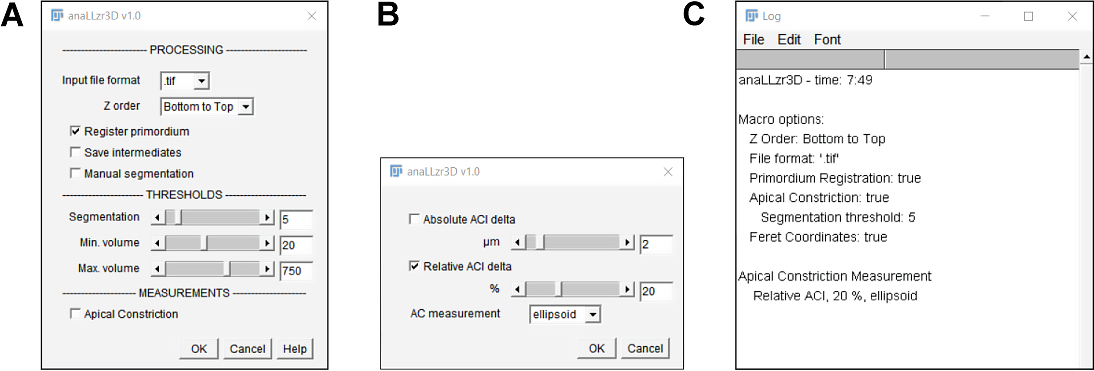
\includegraphics[width=0.95\linewidth]{figures/materials/macros/anallzr3D_macro} 

}

\caption[anaLLzR3D opening dialog]{anaLLzR3D opening dialog \textbf{A} Opening dialog: Main functionality \textbf{B} Opening Dialog: Apical Constriction options \textbf{C} Log window after startup}\label{fig:anallzr3ddialog}
\end{figure}
\hypertarget{image-analysis-1}{%
\subsubsection{Image Analysis}\label{image-analysis-1}}

For pLLP analyses I developed a custom IJ macro script that recognizes cell boundaries \emph{via} the fluorescence signal emitted by a membrane tethered eGFP which expression is controlled by the \emph{claudinB} lateral line specific promotor (\emph{32}). The central IJ tool used to do this is the MorphoLibJ's(\emph{70}) \emph{Morpholigical Segmentation} plugin. The plugin however requires to choose for a `segmentation threshold' that determines the quality and the quantity of segmented objects. This parameter therefore plays an essential role in the reliability of the analysis results.

\hypertarget{registration-1}{%
\paragraph{Registration}\label{registration-1}}

The first module of the macro is the registration of the pLLP in X, Y and cropping in Z. This is accomplished by an initial maximum Z projection and blurring of the image, 2-D segmentation using a minimum threshold and lastly by rotating the segment through the angle formed by the long axis of the ellipsoid (see section \ref{ACI-pol} for more information) and the horizon (at 0\(^{\circ}\)). After rotation the image is cropped according to the obtained ROI, as described before. Additionally, the centers of the most constricting areas are detected \emph{via} an intensity based dynamic threshold and highlighted as magenta circles in figure \ref{fig:maxraw}.


\begin{figure}

{\centering 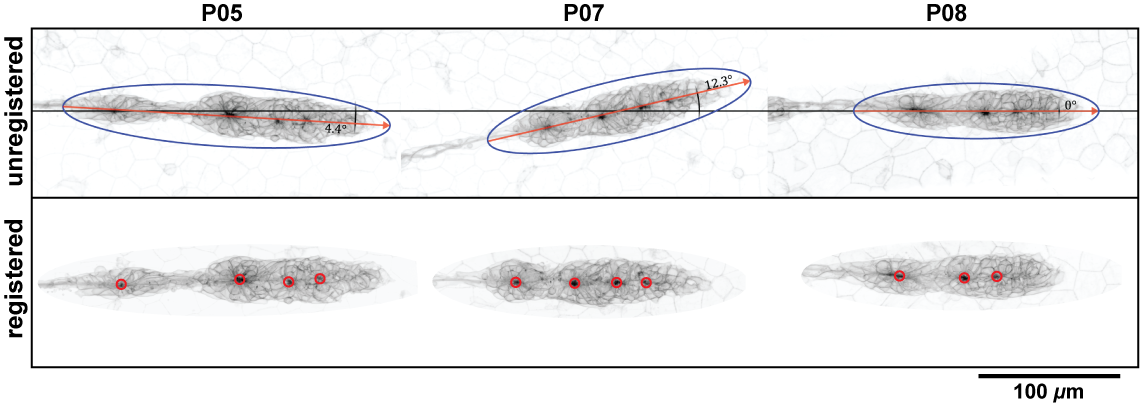
\includegraphics[width=0.95\linewidth]{figures/materials/ground_truth/registration} 

}

\caption[Registration of 3D data]{Registration of 3D data. \textbf{(unregistered)} location and orientation of the unregistered MaxIPs in XY. The red line indicates the angle in degrees from the horizontal midline. The blue oval indicates registration ROI as determined by the macro. \textbf{(registered)} pLLPs after XY transformation took place. red circles indicate rosette centers as detected by the macro based on maximum signal intensity.}\label{fig:maxraw}
\end{figure}
\begin{table}[!h]

\caption{\label{tab:imgprop}3-D Ground Truth image scaling}
\centering
\begin{tabu} to \linewidth {>{\raggedleft}X>{\raggedright}X}
\toprule
\rowcolor{gray!6}  XY resolution & 0.1625 / 0.1625 $\mu$m\\
Z resolution & 0.4 $\mu$m\\
\rowcolor{gray!6}  Time difference between Z-planes in Z & 0.5428 s\\
\bottomrule
\end{tabu}
\end{table}
\hypertarget{image-data}{%
\paragraph{Image data}\label{image-data}}

In figure \ref{fig:stackmem} the fluorescence signal of the three pLLPs used for the Ground-Truth is shown in a single central cross-section along the \emph{dorso-ventral} and the \emph{apico-basal} axis.


\begin{figure}

{\centering 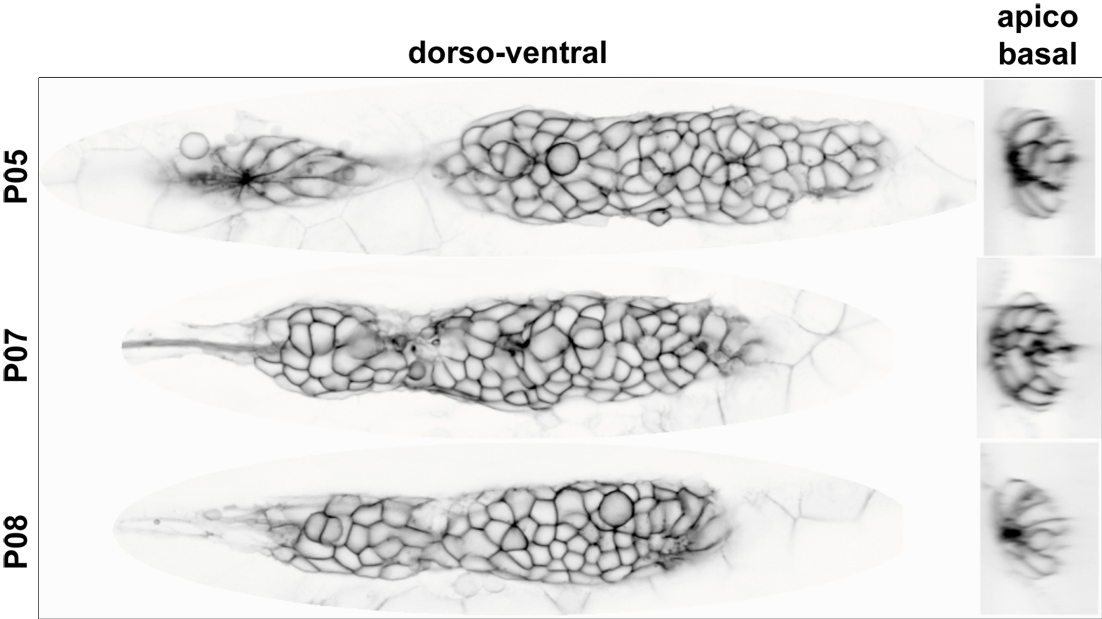
\includegraphics[width=0.7\linewidth]{figures/materials/ground_truth/stackmem} 

}

\caption[Image data pLLP segmentation]{\emph{cldnb:lyn-gfp} fluorescence signal in a cross-section of the pLLP (Obj.: 40X APO, scale bar = 100 \(\mu\)m)}\label{fig:stackmem}
\end{figure}
To compare the results between the Ground Truth segments and the segments obtained from different threshold levels graphically, for a single pLLP the Ground Truth and threshold levels are shown as a composite color image in figure \ref{fig:anallzrvols}. By using a green lookup-table (LUT) for the Ground Truth and a magenta LUT for the threshold level{[}n{]}, one can readily detect overlapping objects (white), over segmentation (magenta) and under segmentation (green). False \emph{positive} segments are cells that are not part of the Ground Truth, including those cells that would distort our dataset. False \emph{nevagtive} segments are cells that are part of the Ground Truth but were not detected by the macro (green cells), excluding those cells impacts the cell count. As one can see, the green cells are randomly distributed, therefore, when averaging a variable for all cells, those cells are less likely to distort our dataset. Only if under segmentation becomes too high will it impact the distribution of values. At Treshold Level 2 (T02) we have the least green cells, but the most magenta cells. At Threshold Level 4 (T04) we have no magenta, but some more green cells. Therefore, to be on the safe side in terms of cell parameters and dataset integrity, for the definition of our Ground Truth T04 would be the best pick.


\begin{figure}

{\centering 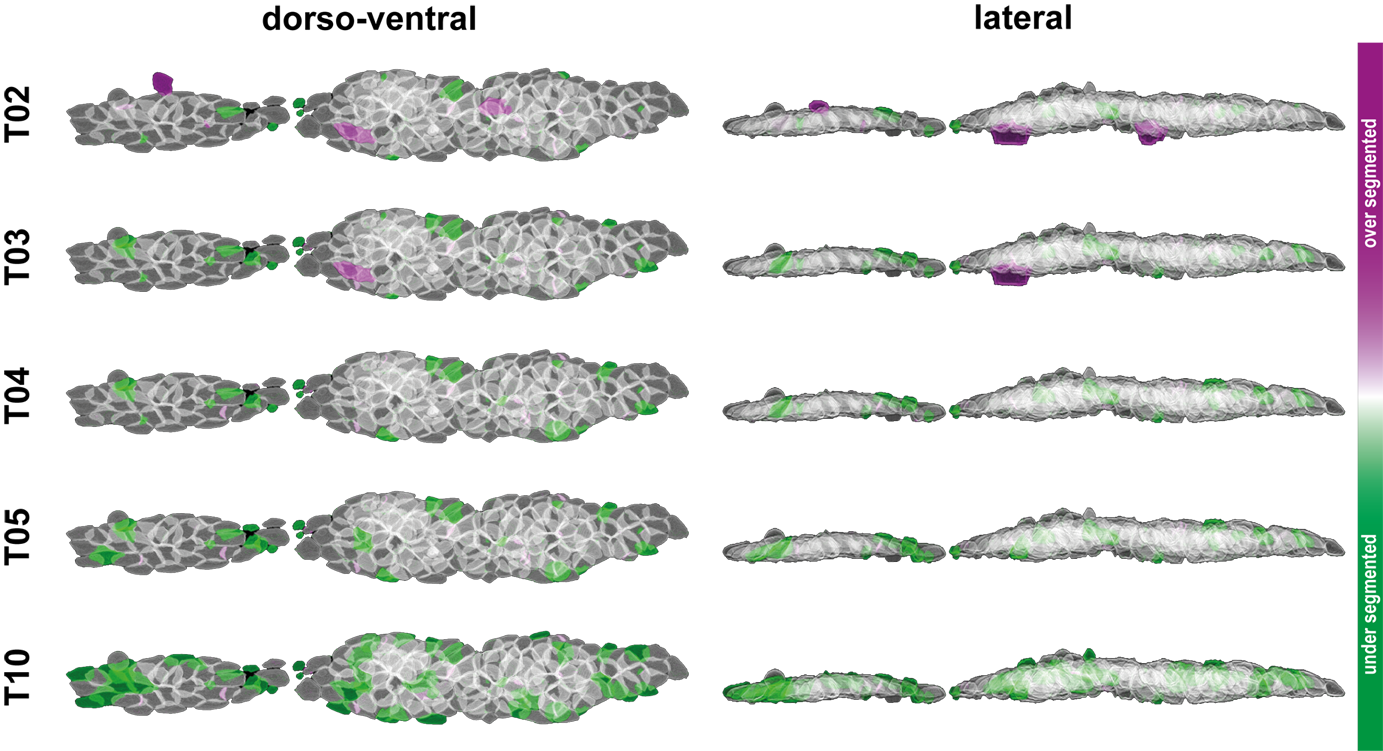
\includegraphics[width=0.85\linewidth]{figures/materials/ground_truth/volumes} 

}

\caption[anaLLzr3D - Graphical comparison of tested thresholds]{Graphical comparison of the thresholds tested. Volume renderings have been done with IJ's \href{\%22https://github.com/fiji/Volume_Viewer/releases/tag/Volume_Viewer-2.01.2\%22}{VolumeViewer}}\label{fig:anallzrvols}
\end{figure}
\noindent 

\hypertarget{code-snippets-1}{%
\subsubsection{Code Snippets}\label{code-snippets-1}}

\hypertarget{registration-2}{%
\paragraph{Registration}\label{registration-2}}

First we need to get parameters angle and height for registration. All steps are performed on Z-projected data.

\scriptsize
\begin{Shaded}
\begin{Highlighting}[numbers=left,,]
\CommentTok{# 2D segmentation mask}
  \KeywordTok{run}\NormalTok{(}\StringTok{"Z Project..."}\NormalTok{, }\StringTok{"projection = [Max Intensity]"}\NormalTok{);}
    \KeywordTok{run}\NormalTok{(}\StringTok{"Gaussian Blur..."}\NormalTok{, }\StringTok{"sigma = 8 scaled"}\NormalTok{);}
    \KeywordTok{setAutoThreshold}\NormalTok{(}\StringTok{"Minimum dark"}\NormalTok{);}
    \KeywordTok{run}\NormalTok{(}\StringTok{"Convert to Mask"}\NormalTok{);}
    \KeywordTok{run}\NormalTok{(}\StringTok{"Select None"}\NormalTok{);}

\CommentTok{# angle from horizontal midline}
    \KeywordTok{run}\NormalTok{(}\StringTok{"Analyze Particles..."}\NormalTok{, }\StringTok{"include add"}\NormalTok{);}
\NormalTok{    rmcount =}\StringTok{ }\KeywordTok{roiManager}\NormalTok{(}\StringTok{"count"}\NormalTok{)}\OperatorTok{-}\DecValTok{1}\NormalTok{;}
    \ControlFlowTok{if}\NormalTok{(}\KeywordTok{roiManager}\NormalTok{(}\StringTok{"count"}\NormalTok{) }\OperatorTok{==}\StringTok{ }\DecValTok{1}\NormalTok{) \{}
        \KeywordTok{roiManager}\NormalTok{(}\StringTok{"select"}\NormalTok{, }\DecValTok{0}\NormalTok{);}
        \KeywordTok{run}\NormalTok{(}\StringTok{"Fit Ellipse"}\NormalTok{);}
\NormalTok{        List.setMeasurements;}
\NormalTok{        Angle =}\StringTok{ }\KeywordTok{List.getValue}\NormalTok{(}\StringTok{"FeretAngle"}\NormalTok{);}
        \ControlFlowTok{if}\NormalTok{ (Angle }\OperatorTok{<}\StringTok{ }\DecValTok{0}\NormalTok{) \{Angle =}\StringTok{ }\NormalTok{Angle }\OperatorTok{*}\StringTok{ }\NormalTok{(}\OperatorTok{-}\DecValTok{1}\NormalTok{);\}}
        \ControlFlowTok{if}\NormalTok{ (Angle }\OperatorTok{>}\StringTok{ }\DecValTok{90}\NormalTok{) \{Angle =}\StringTok{ }\NormalTok{(}\DecValTok{180} \OperatorTok{-}\StringTok{ }\NormalTok{Angle) }\OperatorTok{*}\StringTok{ }\NormalTok{(}\OperatorTok{-}\DecValTok{1}\NormalTok{);\}}
\NormalTok{    \} }\ControlFlowTok{else}\NormalTok{ \{}
        \KeywordTok{roiManager}\NormalTok{(}\StringTok{"select"}\NormalTok{, }\DecValTok{0}\NormalTok{);}
        \KeywordTok{run}\NormalTok{(}\StringTok{"Fit Ellipse"}\NormalTok{);}
        \KeywordTok{roiManager}\NormalTok{(}\StringTok{"update"}\NormalTok{);}
\NormalTok{        List.setMeasurements;}
\NormalTok{        X1Line =}\StringTok{ }\KeywordTok{List.getValue}\NormalTok{(}\StringTok{"X"}\NormalTok{);}
\NormalTok{        Y1Line =}\StringTok{ }\KeywordTok{List.getValue}\NormalTok{(}\StringTok{"Y"}\NormalTok{);}
        \KeywordTok{roiManager}\NormalTok{(}\StringTok{"select"}\NormalTok{, rmcount);}
\NormalTok{        List.setMeasurements;}
\NormalTok{        X2Line =}\StringTok{ }\KeywordTok{List.getValue}\NormalTok{(}\StringTok{"X"}\NormalTok{);}
\NormalTok{        Y2Line =}\StringTok{ }\KeywordTok{List.getValue}\NormalTok{(}\StringTok{"Y"}\NormalTok{);}
        \KeywordTok{makeLine}\NormalTok{(X1Line, Y1Line, X2Line, Y2Line); }
\NormalTok{        List.setMeasurements;}
\NormalTok{        Angle =}\StringTok{ }\KeywordTok{List.getValue}\NormalTok{(}\StringTok{"Angle"}\NormalTok{);}
        \ControlFlowTok{if}\NormalTok{ (Angle }\OperatorTok{<}\StringTok{ }\DecValTok{0}\NormalTok{) \{Angle =}\StringTok{ }\NormalTok{Angle}\OperatorTok{*}\NormalTok{(}\OperatorTok{-}\DecValTok{1}\NormalTok{);\}}
        \ControlFlowTok{if}\NormalTok{ (Angle }\OperatorTok{>}\StringTok{ }\DecValTok{90}\NormalTok{) \{Angle =}\StringTok{ }\NormalTok{(}\DecValTok{180}\OperatorTok{-}\NormalTok{Angle)}\OperatorTok{*}\NormalTok{(}\OperatorTok{-}\DecValTok{1}\NormalTok{);\}}
\NormalTok{    \}}
    \KeywordTok{run}\NormalTok{(}\StringTok{"Select None"}\NormalTok{);}
    \KeywordTok{run}\NormalTok{(}\StringTok{"Rotate... "}\NormalTok{, }\StringTok{"angle = "}\OperatorTok{+}\StringTok{ }\NormalTok{Angle }\OperatorTok{+}\StringTok{" grid = 1 interpolation = Bilinear"}\NormalTok{);}
    
\CommentTok{# height to crop image to}
    \KeywordTok{roiManager}\NormalTok{(}\StringTok{"reset"}\NormalTok{); }\CommentTok{# the image was rotated, so we need to get the ROIs again}
    \KeywordTok{run}\NormalTok{(}\StringTok{"Select None"}\NormalTok{);}
    \KeywordTok{run}\NormalTok{(}\StringTok{"Make Binary"}\NormalTok{);}
    \KeywordTok{run}\NormalTok{(}\StringTok{"Erode"}\NormalTok{);}
    \KeywordTok{run}\NormalTok{(}\StringTok{"Analyze Particles..."}\NormalTok{, }\StringTok{"size = 150-10000 include exclude add"}\NormalTok{);}
\NormalTok{    rmcount =}\StringTok{ }\KeywordTok{roiManager}\NormalTok{(}\StringTok{"count"}\NormalTok{) }\OperatorTok{-}\StringTok{ }\DecValTok{1}\NormalTok{;}
    \ControlFlowTok{if}\NormalTok{(}\KeywordTok{roiManager}\NormalTok{(}\StringTok{"count"}\NormalTok{) }\OperatorTok{==}\StringTok{ }\DecValTok{1}\NormalTok{) \{}
        \KeywordTok{roiManager}\NormalTok{(}\StringTok{"select"}\NormalTok{, }\DecValTok{0}\NormalTok{);}
\NormalTok{    \} }\ControlFlowTok{else}\NormalTok{ \{}
        \KeywordTok{roiManager}\NormalTok{(}\StringTok{"select"}\NormalTok{, rmcount);}
\NormalTok{    \}}
\NormalTok{    List.setMeasurements;}
\NormalTok{    XRect =}\StringTok{ }\KeywordTok{List.getValue}\NormalTok{(}\StringTok{"X"}\NormalTok{);}
\NormalTok{    YRect =}\StringTok{ }\KeywordTok{List.getValue}\NormalTok{(}\StringTok{"Y"}\NormalTok{);}
    \KeywordTok{getDimensions}\NormalTok{(width, height, channels, slices, frames);}
\NormalTok{    Regwidth =}\StringTok{ }\NormalTok{width;}
\NormalTok{    Regheight =}\StringTok{ }\DecValTok{400}\NormalTok{; }\CommentTok{# change height of rectangle here}
    \KeywordTok{toUnscaled}\NormalTok{(YRect);}
\NormalTok{    YRect =}\StringTok{ }\NormalTok{YRect }\OperatorTok{-}\StringTok{ }\NormalTok{(Regheight}\OperatorTok{/}\DecValTok{2}\NormalTok{);}
\end{Highlighting}
\end{Shaded}
\normalsize

\hypertarget{transformation}{%
\paragraph{Transformation}\label{transformation}}

Next we transform our 3D data based on the registration parameters derived from the previous step.

\scriptsize
\begin{Shaded}
\begin{Highlighting}[numbers=left,,]
\CommentTok{# register pLLP}
    \KeywordTok{run}\NormalTok{(}\StringTok{"Rotate... "}\NormalTok{, }\StringTok{"angle = "}\OperatorTok{+}\StringTok{ }\NormalTok{Angle }\OperatorTok{+}\StringTok{" grid = 1 interpolation = Bilinear stack"}\NormalTok{);}
    \KeywordTok{makeRectangle}\NormalTok{(}\DecValTok{0}\NormalTok{, YRect, Regwidth, Regheight);}
    \KeywordTok{run}\NormalTok{(}\StringTok{"Crop"}\NormalTok{);}

\CommentTok{# create threshold mask to clear signals outside ROI}
    \KeywordTok{run}\NormalTok{(}\StringTok{"Normalize Local Contrast"}\NormalTok{, }\StringTok{"block_radius_x = 300 block_radius_y = 20 standard_deviations = 4 stretch"}\NormalTok{);}
    \KeywordTok{run}\NormalTok{(}\StringTok{"Gaussian Blur..."}\NormalTok{, }\StringTok{"sigma = 1 scaled"}\NormalTok{);}
    \KeywordTok{setAutoThreshold}\NormalTok{(}\StringTok{"Otsu dark"}\NormalTok{);}
    \KeywordTok{run}\NormalTok{(}\StringTok{"Convert to Mask"}\NormalTok{);}

\CommentTok{# most right roi}
    \ControlFlowTok{for}\NormalTok{ (}\DataTypeTok{j =} \DecValTok{0}\NormalTok{ ; j }\OperatorTok{<}\StringTok{ }\KeywordTok{roiManager}\NormalTok{(}\StringTok{"count"}\NormalTok{); j}\OperatorTok{++}\NormalTok{) \{}
        \KeywordTok{roiManager}\NormalTok{(}\StringTok{"select"}\NormalTok{, j);}
        \KeywordTok{run}\NormalTok{(}\StringTok{"Set Scale..."}\NormalTok{, }\StringTok{"distance = 1 known = 0.00005 pixel = 1 unit = micron"}\NormalTok{);}
\NormalTok{        List.setMeasurements;}
\NormalTok{    x =}\StringTok{ }\KeywordTok{List.getValue}\NormalTok{(}\StringTok{"X"}\NormalTok{);}
    \KeywordTok{roiManager}\NormalTok{(}\StringTok{"rename"}\NormalTok{, x);}
\NormalTok{    \}}
    \KeywordTok{roiManager}\NormalTok{(}\StringTok{"Sort"}\NormalTok{);}
    \KeywordTok{run}\NormalTok{(}\StringTok{"Properties..."}\NormalTok{, }
        \StringTok{"channels = 1 slices = 1 frames = 1 unit = micron pixel_width = [sizeX] pixel_height = [sizeY] voxel_depth = [sizeZ]"}\NormalTok{);}
\NormalTok{    primroi =}\StringTok{ }\KeywordTok{roiManager}\NormalTok{(}\StringTok{"count"}\NormalTok{) }\OperatorTok{-}\StringTok{ }\DecValTok{1}\NormalTok{;}
    \KeywordTok{roiManager}\NormalTok{(}\StringTok{'select'}\NormalTok{, primroi);}
    
\CommentTok{# enlarge rois to not miss anything}
    \KeywordTok{run}\NormalTok{(}\StringTok{"Enlarge..."}\NormalTok{, }\StringTok{"enlarge = 10"}\NormalTok{);}
    \KeywordTok{run}\NormalTok{(}\StringTok{"Fit Ellipse"}\NormalTok{);}
    \KeywordTok{roiManager}\NormalTok{(}\StringTok{'update'}\NormalTok{);}
\end{Highlighting}
\end{Shaded}
\normalsize

\hypertarget{rosette-detection}{%
\paragraph{Rosette detection}\label{rosette-detection}}

To analyze cells within rosettes resp. within a certain radius of rosettes we first need to know where the rosettes are. At rosette centers we observe an increase in signal intensity since here the membranes of many cells come together in a very small area. This effect we can use to utilize a maximum finder algorithm together with a threshold that is defined individually for each image.

\scriptsize
\begin{Shaded}
\begin{Highlighting}[numbers=left,,]
\CommentTok{#  [...] registration}
    \KeywordTok{run}\NormalTok{(}\StringTok{"Gaussian Blur..."}\NormalTok{, }\StringTok{"sigma = 4 scaled"}\NormalTok{);}
\NormalTok{    List.setMeasurements;}
\NormalTok{    mean =}\StringTok{ }\KeywordTok{List.getValue}\NormalTok{(}\StringTok{"Mean"}\NormalTok{);}
\NormalTok{    pointthresh =}\StringTok{ }\NormalTok{mean}\OperatorTok{/}\FloatTok{2.5}\NormalTok{;}
\NormalTok{    pointthresh =}\StringTok{ }\KeywordTok{round}\NormalTok{(pointthresh);}
    \KeywordTok{run}\NormalTok{(}\StringTok{"Find Maxima..."}\NormalTok{, }\StringTok{"noise = "}\OperatorTok{+}\StringTok{ }\NormalTok{pointthresh }\OperatorTok{+}\StringTok{" output = [Point Selection]"}\NormalTok{);}
    \KeywordTok{run}\NormalTok{(}\StringTok{"Point Tool..."}\NormalTok{, }\StringTok{"type = Dot color = Green size = [Extra Large] label counter = 0"}\NormalTok{);}
    \KeywordTok{getSelectionCoordinates}\NormalTok{(xpoints, ypoints);}
    \KeywordTok{roiManager}\NormalTok{(}\StringTok{"Add"}\NormalTok{);}

\CommentTok{# measure intensities along horizontal midline}
\CommentTok{#   [...] registration}
\NormalTok{    Rlx =}\StringTok{ }\KeywordTok{lengthOf}\NormalTok{(xpoints); }\CommentTok{# collect Arrays}
\NormalTok{    RX =}\StringTok{ }\KeywordTok{Array.sort}\NormalTok{(xpoints); }\CommentTok{# put xpoints in right order}
\NormalTok{    RX =}\StringTok{ }\KeywordTok{Array.invert}\NormalTok{(RX);}

\CommentTok{# fill ypoints with mean values of all y coordinates}
    \KeywordTok{Array.getStatistics}\NormalTok{(ypoints, min, max, mean, stdDev);}
\NormalTok{    meanline =}\StringTok{ }\NormalTok{mean;}
    \KeywordTok{Array.fill}\NormalTok{(ypoints, meanline);}
\NormalTok{    RY =}\StringTok{ }\NormalTok{ypoints;}
    \KeywordTok{getDimensions}\NormalTok{(width, height, channels, slices, frames);}
    \KeywordTok{makeLine}\NormalTok{(}\DecValTok{0}\NormalTok{, meanline, width, meanline, }\DecValTok{1}\NormalTok{);}
    \KeywordTok{run}\NormalTok{(}\StringTok{"Clear Results"}\NormalTok{);}
\NormalTok{    profile =}\StringTok{ }\KeywordTok{getProfile}\NormalTok{();}
    \ControlFlowTok{for}\NormalTok{ (}\DataTypeTok{a =} \DecValTok{0}\NormalTok{; a }\OperatorTok{<}\StringTok{ }\NormalTok{profile.length; a}\OperatorTok{++}\NormalTok{) \{}
    \KeywordTok{setResult}\NormalTok{(}\StringTok{"Value"}\NormalTok{, a, profile[a]);}
        \KeywordTok{updateResults}\NormalTok{();}
\NormalTok{    \}}
\end{Highlighting}
\end{Shaded}
\normalsize

\hypertarget{segmentation-2}{%
\paragraph{Segmentation}\label{segmentation-2}}

For image segmentation we use the MorphoLibJ's(\emph{70}) \emph{Morpholigical Segmentation} plugin. Function calls and arguments are defined in the publication documentation.

\scriptsize
\begin{Shaded}
\begin{Highlighting}[numbers=left,,]
\CommentTok{# 3D gaussian blur}
    \KeywordTok{run}\NormalTok{(}\StringTok{"Gaussian Blur 3D..."}\NormalTok{, }\StringTok{"x=2 y=2 z=0.5"}\NormalTok{);}
    \KeywordTok{resetMinAndMax}\NormalTok{();}

\CommentTok{# run segmentation}
    \KeywordTok{run}\NormalTok{(}\StringTok{"Morphological Segmentation"}\NormalTok{);}
    \KeywordTok{selectWindow}\NormalTok{(}\StringTok{"Morphological Segmentation"}\NormalTok{);}
    \KeywordTok{call}\NormalTok{(}\StringTok{"inra.ijpb.plugins.MorphologicalSegmentation.setInputImageType"}\NormalTok{, }\StringTok{"border"}\NormalTok{);}
    \KeywordTok{call}\NormalTok{(}\StringTok{"inra.ijpb.plugins.MorphologicalSegmentation.segment"}\NormalTok{, }\StringTok{"tolerance = "}\OperatorTok{+}\StringTok{ }\NormalTok{tol}\OperatorTok{+}\StringTok{""}\NormalTok{,}
         \StringTok{"calculateDams = true"}\NormalTok{, }\StringTok{"connectivity = 6"}\NormalTok{);}

\CommentTok{# wait till segmentation is done}
\NormalTok{    initTime =}\StringTok{ }\KeywordTok{getTime}\NormalTok{(); }
\NormalTok{  oldTime =}\StringTok{ }\NormalTok{initTime; }
    \ControlFlowTok{while}\NormalTok{ (}\KeywordTok{isOpen}\NormalTok{(}\StringTok{"Morphological Segmentation"}\NormalTok{)) \{}
\NormalTok{      elapsedTime =}\StringTok{ }\KeywordTok{getTime}\NormalTok{() }\OperatorTok{-}\StringTok{ }\NormalTok{initTime; }
\NormalTok{        newTime =}\StringTok{ }\KeywordTok{getTime}\NormalTok{() }\OperatorTok{-}\StringTok{ }\NormalTok{oldTime;}
        \ControlFlowTok{if}\NormalTok{ (newTime }\OperatorTok{>}\StringTok{ }\DecValTok{10000}\NormalTok{) \{}
\NormalTok{        oldTime =}\StringTok{ }\KeywordTok{getTime}\NormalTok{(); }
\NormalTok{        newTime =}\StringTok{ }\DecValTok{0}\NormalTok{;}
\NormalTok{        loginfo =}\StringTok{ }\KeywordTok{getInfo}\NormalTok{(}\StringTok{"log"}\NormalTok{);}
\NormalTok{            loginfo =}\StringTok{ }\KeywordTok{split}\NormalTok{(loginfo, }\StringTok{" "}\NormalTok{);}
\NormalTok{            loginfo =}\StringTok{ }\KeywordTok{Array.reverse}\NormalTok{(loginfo);}
\NormalTok{            loginfo =}\StringTok{ }\KeywordTok{Array.trim}\NormalTok{(loginfo, }\DecValTok{5}\NormalTok{);}
\NormalTok{            loginfo =}\StringTok{ }\KeywordTok{Array.reverse}\NormalTok{(loginfo);}
\NormalTok{            loginfo =}\StringTok{ }\KeywordTok{split}\NormalTok{(loginfo[}\DecValTok{0}\NormalTok{], }\StringTok{"."}\NormalTok{);}
\NormalTok{            loginfo =}\StringTok{ }\KeywordTok{Array.reverse}\NormalTok{(loginfo);}
\NormalTok{            loginfo =}\StringTok{ }\NormalTok{loginfo[}\DecValTok{0}\NormalTok{];}
            \ControlFlowTok{if}\NormalTok{ (loginfo }\OperatorTok{==}\StringTok{ "}\CharTok{\textbackslash{}n}\StringTok{Whole"}\NormalTok{) \{}
                \KeywordTok{call}\NormalTok{(}\StringTok{"inra.ijpb.plugins.MorphologicalSegmentation.setDisplayFormat"}\NormalTok{, }\StringTok{"Catchment basins"}\NormalTok{);}
                \KeywordTok{call}\NormalTok{(}\StringTok{"inra.ijpb.plugins.MorphologicalSegmentation.createResultImage"}\NormalTok{);}
                \KeywordTok{run}\NormalTok{(}\StringTok{"Grays"}\NormalTok{);}
                \KeywordTok{selectWindow}\NormalTok{(}\StringTok{"Morphological Segmentation"}\NormalTok{);}
                \KeywordTok{close}\NormalTok{();}
\NormalTok{            \}}
\NormalTok{    \}}
\NormalTok{    \}}
  \KeywordTok{run}\NormalTok{(}\StringTok{"Properties..."}\NormalTok{, }\StringTok{"channels = 1 slices = "}\OperatorTok{+}\StringTok{ }\NormalTok{n }\OperatorTok{+}\StringTok{" frames = 1 unit = microns pixel_width="}\OperatorTok{+}\StringTok{ }
\StringTok{        }\NormalTok{sizeX }\OperatorTok{+}\StringTok{" pixel_height="}\OperatorTok{+}\StringTok{ }\NormalTok{sizeY }\OperatorTok{+}\StringTok{ "voxel_depth ="}\OperatorTok{+}\StringTok{ }\NormalTok{sizeZ);}
\end{Highlighting}
\end{Shaded}
\normalsize

\hypertarget{filter-and-clearing}{%
\paragraph{Filter and clearing}\label{filter-and-clearing}}

Remove segments below a certain volume threshold defined in the startup dialog and clear blank slices in Z.

\scriptsize
\begin{Shaded}
\begin{Highlighting}[numbers=left,,]
\CommentTok{# erase objects V < vmin and V > vmax}
  \KeywordTok{run}\NormalTok{(}\StringTok{"3D Manager Options"}\NormalTok{, }\StringTok{"volume surface compactness fit_ellipse 3d_moments }
\StringTok{      feret centroid_(pix) centroid_(unit) distance_to_surface centre_of_mass_(unit) }
\StringTok{      bounding_box radial_distance surface_contact closest exclude_objects_on_edges_xy }
\StringTok{      sync distance_between_centers = 10 distance_max_contact = 1.80"}\NormalTok{);}
    \KeywordTok{run}\NormalTok{(}\StringTok{"3D Manager"}\NormalTok{);}
  \KeywordTok{selectWindow}\NormalTok{(OMap);}
    \KeywordTok{Ext.Manager3D_AddImage}\NormalTok{();}

\CommentTok{# get number of objects}
    \KeywordTok{Ext.Manager3D_Count}\NormalTok{(nb);}
    \KeywordTok{Ext.Manager3D_MultiSelect}\NormalTok{();}

\CommentTok{# loop through all the objects and erase by filter settings}
    \ControlFlowTok{for}\NormalTok{(}\DataTypeTok{k =} \DecValTok{0}\NormalTok{; k }\OperatorTok{<}\StringTok{ }\NormalTok{nb; k}\OperatorTok{++}\NormalTok{) \{}
        \KeywordTok{showStatus}\NormalTok{(}\StringTok{"Processing "}\OperatorTok{+}\StringTok{ }\NormalTok{k }\OperatorTok{+}\StringTok{"/"}\OperatorTok{+}\StringTok{ }\NormalTok{nb);}
        \KeywordTok{Ext.Manager3D_Measure3D}\NormalTok{(k, }\StringTok{"Vol"}\NormalTok{,V);}
        \ControlFlowTok{if}\NormalTok{ (V }\OperatorTok{<}\StringTok{ }\NormalTok{vmin) \{}
            \KeywordTok{Ext.Manager3D_Select}\NormalTok{(k);}
            \KeywordTok{Ext.Manager3D_Erase}\NormalTok{();}
            \ControlFlowTok{if}\NormalTok{ (V }\OperatorTok{>}\StringTok{ }\NormalTok{vmax) \{}
                \KeywordTok{Ext.Manager3D_Select}\NormalTok{(k);}
                \KeywordTok{Ext.Manager3D_Erase}\NormalTok{();}
\NormalTok{            \}}
\NormalTok{        \}}
\NormalTok{    \}}

\CommentTok{# clean blank slices from bottom and top}
    \KeywordTok{getDimensions}\NormalTok{(width, height, channels, slices, frames);}
\NormalTok{    var done =}\StringTok{ }\NormalTok{false; }
    \ControlFlowTok{for}\NormalTok{(}\DataTypeTok{l =} \DecValTok{1}\NormalTok{; l }\OperatorTok{<}\StringTok{ }\NormalTok{slices }\OperatorTok{&&!}\NormalTok{done; l}\OperatorTok{++}\NormalTok{) \{}
        \KeywordTok{setSlice}\NormalTok{(l);}
        \KeywordTok{getStatistics}\NormalTok{(area, mean, min, max, std, histogram);}
        \ControlFlowTok{if}\NormalTok{(max }\OperatorTok{>}\StringTok{ }\DecValTok{0}\NormalTok{) \{}
\NormalTok{        amax =}\StringTok{ }\NormalTok{l}\DecValTok{-1}\NormalTok{;}
            \KeywordTok{run}\NormalTok{(}\StringTok{"Slice Remover"}\NormalTok{, }\StringTok{"first = 1 last = "}\OperatorTok{+}\StringTok{ }\NormalTok{amax }\OperatorTok{+}\StringTok{" increment = 1"}\NormalTok{);}
            \KeywordTok{run}\NormalTok{(}\StringTok{"Reverse"}\NormalTok{);}
            \KeywordTok{getDimensions}\NormalTok{(width, height, channels, slices, frames);}
            \ControlFlowTok{for}\NormalTok{(}\DataTypeTok{l =} \DecValTok{1}\NormalTok{; l }\OperatorTok{<}\StringTok{ }\NormalTok{slices }\OperatorTok{&&!}\NormalTok{done; l}\OperatorTok{++}\NormalTok{) \{}
                \KeywordTok{setSlice}\NormalTok{(l);}
                \KeywordTok{getStatistics}\NormalTok{(area, mean, min, max, std, histogram);}
                \ControlFlowTok{if}\NormalTok{(max }\OperatorTok{>}\StringTok{ }\DecValTok{0}\NormalTok{) \{}
\NormalTok{                bmax =}\StringTok{ }\NormalTok{l}\DecValTok{-1}\NormalTok{;}
                    \KeywordTok{run}\NormalTok{(}\StringTok{"Slice Remover"}\NormalTok{, }\StringTok{"first = 1 last = "}\OperatorTok{+}\StringTok{ }\NormalTok{bmax }\OperatorTok{+}\StringTok{" increment = 1"}\NormalTok{);}
                    \KeywordTok{run}\NormalTok{(}\StringTok{"Reverse"}\NormalTok{);}
\NormalTok{                    done =}\StringTok{ }\NormalTok{true;}
\NormalTok{                    \}}
\NormalTok{            \}}
\NormalTok{        \}}
\NormalTok{    \}}
\end{Highlighting}
\end{Shaded}
\normalsize

\hypertarget{apical-constriction-1}{%
\paragraph{Apical Constriction}\label{apical-constriction-1}}

Next we navigate to the calculated relative distance from the apical site and take measurements.

\scriptsize
\begin{Shaded}
\begin{Highlighting}[numbers=left,,]
\CommentTok{# define Z values}
    \ControlFlowTok{if}\NormalTok{ (rosAC) \{}
\NormalTok{        cellum =}\StringTok{ }\NormalTok{rosum; }\CommentTok{# I copy pasted the code, so rosette um would be cell um}
\NormalTok{        Zslice =}\StringTok{ }\NormalTok{rosum}\OperatorTok{/}\NormalTok{sizeZ;}
        \KeywordTok{round}\NormalTok{(Zslice);}
\NormalTok{    \}}
\CommentTok{# cell Constriction}

    \ControlFlowTok{if}\NormalTok{ (cellAC) \{}
\NormalTok{        aciza =}\StringTok{ }\NormalTok{cellum }\OperatorTok{/}\StringTok{ }\NormalTok{sizeZ;}
\NormalTok{        Zslice =}\StringTok{ }\NormalTok{aciza;}
        \KeywordTok{round}\NormalTok{(Zslice);}
        \KeywordTok{round}\NormalTok{(aciza);}
        \ControlFlowTok{if}\NormalTok{ (fixAC}\OperatorTok{||}\NormalTok{symAC) \{}
    \CommentTok{# crop single objects and measure ----------------------}
      \KeywordTok{selectWindow}\NormalTok{(OMap);}
        \KeywordTok{run}\NormalTok{(}\StringTok{"3D Manager Options"}\NormalTok{, }\StringTok{"volume surface compactness fit_ellipse 3d_moments }
\StringTok{        feret centroid_(pix) centroid_(unit) distance_to_surface centre_of_mass_(unit) }
\StringTok{        bounding_box radial_distance surface_contact closest exclude_objects_on_edges_xy }
\StringTok{        sync distance_between_centers = 10 distance_max_contact = 1.80"}\NormalTok{);}
        \KeywordTok{run}\NormalTok{(}\StringTok{"3D Manager"}\NormalTok{);}
        \KeywordTok{Ext.Manager3D_AddImage}\NormalTok{();}
    \CommentTok{# get number of objects}
        \KeywordTok{Ext.Manager3D_Count}\NormalTok{(nb);}
    \CommentTok{# create arrays to fill with measurements}
\NormalTok{        objlabelArray =}\StringTok{ }\KeywordTok{newArray}\NormalTok{(nb);}
\NormalTok{        MajorAngle =}\StringTok{ }\KeywordTok{newArray}\NormalTok{(nb);}
\NormalTok{        ACIMajor =}\StringTok{ }\KeywordTok{newArray}\NormalTok{(nb);}
\NormalTok{        ACIMinor =}\StringTok{ }\KeywordTok{newArray}\NormalTok{(nb);}
\NormalTok{        Dap =}\StringTok{ }\KeywordTok{newArray}\NormalTok{(nb);}
        \KeywordTok{Ext.Manager3D_MultiSelect}\NormalTok{();}
        \ControlFlowTok{for}\NormalTok{(}\DataTypeTok{k =} \DecValTok{0}\NormalTok{; k }\OperatorTok{<}\StringTok{ }\NormalTok{nb; k}\OperatorTok{++}\NormalTok{) \{}
            \ControlFlowTok{if}\NormalTok{ (k }\OperatorTok{>}\StringTok{ }\DecValTok{0}\NormalTok{) \{}
              \KeywordTok{Ext.Manager3D_AddImage}\NormalTok{();}
\NormalTok{            \}}
        \KeywordTok{Ext.Manager3D_GetName}\NormalTok{(k, obj);}
        \KeywordTok{Ext.Manager3D_Centroid3D}\NormalTok{(k, cx, cy, cz);}
    \CommentTok{# measure feret}
        \ControlFlowTok{if}\NormalTok{ (symAC) \{}
          \KeywordTok{Ext.Manager3D_Measure3D}\NormalTok{(k, }\StringTok{"Feret"}\NormalTok{, ferr); }
\NormalTok{            da =}\StringTok{ }\NormalTok{ferr }\OperatorTok{*}\StringTok{ }\NormalTok{cellum;}
\NormalTok{            da =}\StringTok{ }\KeywordTok{round}\NormalTok{(da);}
          \ControlFlowTok{if}\NormalTok{ (da }\OperatorTok{==}\StringTok{ }\DecValTok{0}\NormalTok{) \{}
\NormalTok{              da =}\StringTok{ }\DecValTok{1}\NormalTok{;}
\NormalTok{          \}}
\NormalTok{        Dap[k] =}\StringTok{ }\NormalTok{da;}
\NormalTok{        \}}
        \KeywordTok{toString}\NormalTok{(obj);}
\NormalTok{        objlabelArray[k] =}\StringTok{ }\NormalTok{obj;}
    \CommentTok{# erase all objects except current(k)}
        \KeywordTok{Ext.Manager3D_SelectAll}\NormalTok{();}
        \KeywordTok{Ext.Manager3D_Select}\NormalTok{(k);}
        \KeywordTok{Ext.Manager3D_Erase}\NormalTok{();}
        \KeywordTok{run}\NormalTok{(}\StringTok{"Enhance Contrast..."}\NormalTok{, }\StringTok{"saturated = 0.3 equalize process_all"}\NormalTok{);}
        \KeywordTok{run}\NormalTok{(}\StringTok{"8-bit"}\NormalTok{);}
        \KeywordTok{run}\NormalTok{(}\StringTok{"Crop Label"}\NormalTok{, }\StringTok{"label=255 border=5"}\NormalTok{);}
    \CommentTok{# clear cell stack in Z}
        \KeywordTok{getDimensions}\NormalTok{(width, height, channels, slices, frames);}
\NormalTok{        var done =}\StringTok{ }\NormalTok{false; }
        \ControlFlowTok{for}\NormalTok{(}\DataTypeTok{l =} \DecValTok{1}\NormalTok{; l }\OperatorTok{<}\StringTok{ }\NormalTok{slices }\OperatorTok{&&!}\NormalTok{done; l}\OperatorTok{++}\NormalTok{) \{}
          \KeywordTok{setSlice}\NormalTok{(l);}
            \KeywordTok{getStatistics}\NormalTok{(area, mean, min, max, std, histogram);}
            \ControlFlowTok{if}\NormalTok{(max }\OperatorTok{>}\StringTok{ }\DecValTok{0}\NormalTok{) \{ }\OperatorTok{/}\ErrorTok{/}\StringTok{ }\NormalTok{from apical}
\NormalTok{            smax =}\StringTok{ }\NormalTok{l}\DecValTok{-1}\NormalTok{;}
            \KeywordTok{run}\NormalTok{(}\StringTok{"Slice Remover"}\NormalTok{, }\StringTok{"first=1 last="}\OperatorTok{+}\NormalTok{smax}\OperatorTok{+}\StringTok{" increment=1"}\NormalTok{);}
            \KeywordTok{run}\NormalTok{(}\StringTok{"Reverse"}\NormalTok{);}
            \KeywordTok{getDimensions}\NormalTok{(width, height, channels, slices, frames);}
            \ControlFlowTok{for}\NormalTok{(}\DataTypeTok{l =} \DecValTok{1}\NormalTok{; l }\OperatorTok{<}\StringTok{ }\NormalTok{slices }\OperatorTok{&&!}\NormalTok{done; l}\OperatorTok{++}\NormalTok{) \{ }\OperatorTok{/}\ErrorTok{/}\StringTok{ }\NormalTok{from basal}
                  \KeywordTok{setSlice}\NormalTok{(l);}
                    \KeywordTok{getStatistics}\NormalTok{(area, mean, min, max, std, histogram);}
                    \ControlFlowTok{if}\NormalTok{(max }\OperatorTok{>}\StringTok{ }\DecValTok{0}\NormalTok{) \{}
\NormalTok{                      smax =}\StringTok{ }\NormalTok{l}\DecValTok{-1}\NormalTok{;}
                        \KeywordTok{run}\NormalTok{(}\StringTok{"Slice Remover"}\NormalTok{, }\StringTok{"first = 1 last = "}\OperatorTok{+}\StringTok{ }\NormalTok{smax }\OperatorTok{+}\StringTok{" increment = 1"}\NormalTok{);}
                        \KeywordTok{run}\NormalTok{(}\StringTok{"Reverse"}\NormalTok{);}
\NormalTok{                        done =}\StringTok{ }\NormalTok{true;}
\NormalTok{                    \}}
\NormalTok{                \}}
\NormalTok{            \}}
\NormalTok{        \}}
\NormalTok{        naci =}\StringTok{ }\KeywordTok{nSlices}\NormalTok{();}
\NormalTok{        nacimax =}\StringTok{ }\NormalTok{naci}\OperatorTok{/}\DecValTok{2}\NormalTok{;}
        \KeywordTok{run}\NormalTok{(}\StringTok{"Properties..."}\NormalTok{, }\StringTok{"channels = 1 slices = "}\OperatorTok{+}\StringTok{ }\NormalTok{naci }\OperatorTok{+}\StringTok{" frames = 1 unit = microns }
\StringTok{            pixel_width = "}\OperatorTok{+}\StringTok{ }\NormalTok{sizeX }\OperatorTok{+}\StringTok{" pixel_height = "}\OperatorTok{+}\StringTok{ }\NormalTok{sizeY }\OperatorTok{+}\StringTok{" voxel_depth = "}\OperatorTok{+}\StringTok{ }\NormalTok{sizeZ);}
        \ControlFlowTok{if}\NormalTok{ (symAC) \{}
\NormalTok{            aciza =}\StringTok{ }\NormalTok{da }\OperatorTok{/}\StringTok{ }\NormalTok{sizeZ;}
\NormalTok{            db =}\StringTok{ }\NormalTok{naci }\OperatorTok{-}\StringTok{ }\NormalTok{da;}
\NormalTok{        \}}
    \CommentTok{# if fixed ACI}
        \ControlFlowTok{if}\NormalTok{ (aciza }\OperatorTok{<}\StringTok{ }\NormalTok{(nacimax)) \{}
\NormalTok{          acizb =}\StringTok{ }\NormalTok{naci }\OperatorTok{-}\StringTok{ }\NormalTok{aciza;}
    \CommentTok{# measure apical}
        \KeywordTok{run}\NormalTok{(}\StringTok{"Make Binary"}\NormalTok{, }\StringTok{"method = Default background=Default calculate black"}\NormalTok{);}
        \KeywordTok{setSlice}\NormalTok{(aciza);}
        \KeywordTok{run}\NormalTok{(}\StringTok{"Set Measurements..."}\NormalTok{, }\StringTok{"area centroid bounding fit feret's redirect = None decimal = 2"}\NormalTok{);}
        \KeywordTok{run}\NormalTok{(}\StringTok{"Analyze Particles..."}\NormalTok{, }\StringTok{"display slice"}\NormalTok{);}
    \CommentTok{# get angle}
\NormalTok{        MajorAngle[k] =}\StringTok{ }\KeywordTok{getResult}\NormalTok{(}\StringTok{"FeretAngle"}\NormalTok{, }\DecValTok{0}\NormalTok{);}
        \ControlFlowTok{if}\NormalTok{ (MajorAngle[k] }\OperatorTok{>}\StringTok{ }\DecValTok{90}\NormalTok{) \{}
\NormalTok{          MajorAngle[k] =}\StringTok{ }\DecValTok{90} \OperatorTok{-}\StringTok{ }\NormalTok{(MajorAngle[k] }\OperatorTok{-}\StringTok{ }\DecValTok{90}\NormalTok{);}
\NormalTok{        \}}
    \CommentTok{# get min feret / major / minor}
\NormalTok{        resultsArray =}\StringTok{ }\KeywordTok{newArray}\NormalTok{(}\KeywordTok{nResults}\NormalTok{());}
            \ControlFlowTok{for}\NormalTok{(}\DataTypeTok{p =} \DecValTok{0}\NormalTok{; p }\OperatorTok{<}\StringTok{ }\KeywordTok{nResults}\NormalTok{(); p}\OperatorTok{++}\NormalTok{) \{ }
\NormalTok{            resultsArray[p] =}\StringTok{ }\KeywordTok{getResult}\NormalTok{(}\StringTok{"Minor"}\NormalTok{, p); }
\NormalTok{            \}}
\NormalTok{            total =}\StringTok{ }\DecValTok{0}\NormalTok{; }
            \ControlFlowTok{for}\NormalTok{(}\DataTypeTok{p =} \DecValTok{0}\NormalTok{; p }\OperatorTok{<}\StringTok{ }\KeywordTok{nResults}\NormalTok{(); p}\OperatorTok{++}\NormalTok{) \{ }
\NormalTok{                total =}\StringTok{ }\NormalTok{total }\OperatorTok{+}\StringTok{ }\NormalTok{resultsArray[p]; }
\NormalTok{            \}}
\end{Highlighting}
\end{Shaded}
\normalsize

\hypertarget{single-cell-measurement}{%
\paragraph{Single cell measurement}\label{single-cell-measurement}}

Get 3D measurements from each object using the 3D Manager plugin

\scriptsize
\begin{Shaded}
\begin{Highlighting}[numbers=left,,]
\KeywordTok{run}\NormalTok{(}\StringTok{"3D Manager Options"}\NormalTok{, }\StringTok{"volume surface compactness fit_ellipse 3d_moments }
\StringTok{    feret centroid_(pix) centroid_(unit) distance_to_surface centre_of_mass_(unit) }
\StringTok{    bounding_box radial_distance surface_contact closest exclude_objects_on_edges_xy }
\StringTok{    sync distance_between_centers=10 distance_max_contact = 1.80"}\NormalTok{);}
\KeywordTok{run}\NormalTok{(}\StringTok{"3D Manager"}\NormalTok{);}
\KeywordTok{Ext.Manager3D_AddImage}\NormalTok{();}
\KeywordTok{Ext.Manager3D_DeselectAll}\NormalTok{();}
\KeywordTok{Ext.Manager3D_Measure}\NormalTok{();}
\KeywordTok{Ext.Manager3D_SaveResult}\NormalTok{(}\StringTok{"M"}\NormalTok{, datcelldir }\OperatorTok{+}\StringTok{ }\NormalTok{name }\OperatorTok{+}\StringTok{ ".csv"}\NormalTok{);}
\KeywordTok{Ext.Manager3D_CloseResult}\NormalTok{(}\StringTok{"M"}\NormalTok{);}
\KeywordTok{Ext.Manager3D_Reset}\NormalTok{();}
\KeywordTok{Ext.Manager3D_Close}\NormalTok{();}
\end{Highlighting}
\end{Shaded}
\normalsize

\hypertarget{functions}{%
\paragraph{Functions}\label{functions}}

\scriptsize
\begin{Shaded}
\begin{Highlighting}[numbers=left,,]
\ControlFlowTok{function} \KeywordTok{sliceclear}\NormalTok{() \{}
  \ControlFlowTok{for}\NormalTok{ (}\DataTypeTok{j =} \DecValTok{1}\NormalTok{; j }\OperatorTok{<=}\StringTok{ }\NormalTok{n; j}\OperatorTok{++}\NormalTok{) \{}
    \KeywordTok{roiManager}\NormalTok{(}\StringTok{"reset"}\NormalTok{);}
    \KeywordTok{setSlice}\NormalTok{(j);}
    \KeywordTok{run}\NormalTok{(}\StringTok{"Analyze Particles..."}\NormalTok{, }\StringTok{"include add slice"}\NormalTok{);}
    \ControlFlowTok{if}\NormalTok{ (}\KeywordTok{roiManager}\NormalTok{(}\StringTok{"count"}\NormalTok{) }\OperatorTok{==}\StringTok{ }\DecValTok{0}\NormalTok{) \{}
        \KeywordTok{setSlice}\NormalTok{(j);}
        \KeywordTok{makeRectangle}\NormalTok{(}\DecValTok{0}\NormalTok{, }\DecValTok{0}\NormalTok{, width, height);}
        \KeywordTok{run}\NormalTok{(}\StringTok{"Cut"}\NormalTok{);}
\NormalTok{    \}}
    \ControlFlowTok{if}\NormalTok{ (}\KeywordTok{roiManager}\NormalTok{(}\StringTok{"count"}\NormalTok{) }\OperatorTok{==}\StringTok{ }\DecValTok{1}\NormalTok{) \{}
        \KeywordTok{setSlice}\NormalTok{(j);}
        \KeywordTok{allroi}\NormalTok{();}
        \KeywordTok{wait}\NormalTok{(}\DecValTok{200}\NormalTok{);}
        \KeywordTok{run}\NormalTok{(}\StringTok{"Clear Outside"}\NormalTok{, }\StringTok{"slice"}\NormalTok{);}
\NormalTok{    \}}
    \ControlFlowTok{if}\NormalTok{ (}\KeywordTok{roiManager}\NormalTok{(}\StringTok{"count"}\NormalTok{) }\OperatorTok{>}\StringTok{ }\DecValTok{1}\NormalTok{) \{}
        \KeywordTok{setSlice}\NormalTok{(j);}
        \KeywordTok{allroi}\NormalTok{();}
        \KeywordTok{roiManager}\NormalTok{(}\StringTok{"Combine"}\NormalTok{);}
        \KeywordTok{run}\NormalTok{(}\StringTok{"Clear Outside"}\NormalTok{, }\StringTok{"slice"}\NormalTok{);}
\NormalTok{    \}}
\NormalTok{  \}}
\NormalTok{\}}
\end{Highlighting}
\end{Shaded}
\normalsize

\hypertarget{data-analysis-1}{%
\subsubsection{Data Analysis}\label{data-analysis-1}}

\hypertarget{cell-count}{%
\paragraph{Cell Count}\label{cell-count}}

In figure \ref{fig:gtratio} the relative numbers for each threshold level can be seen in percentage above or below the mean cell count of the ground truth (blue horizon). Analogous to the graphical inspection, the magenta area represents over segmentation, the green under segmentation.


\begin{figure}[H]

{\centering 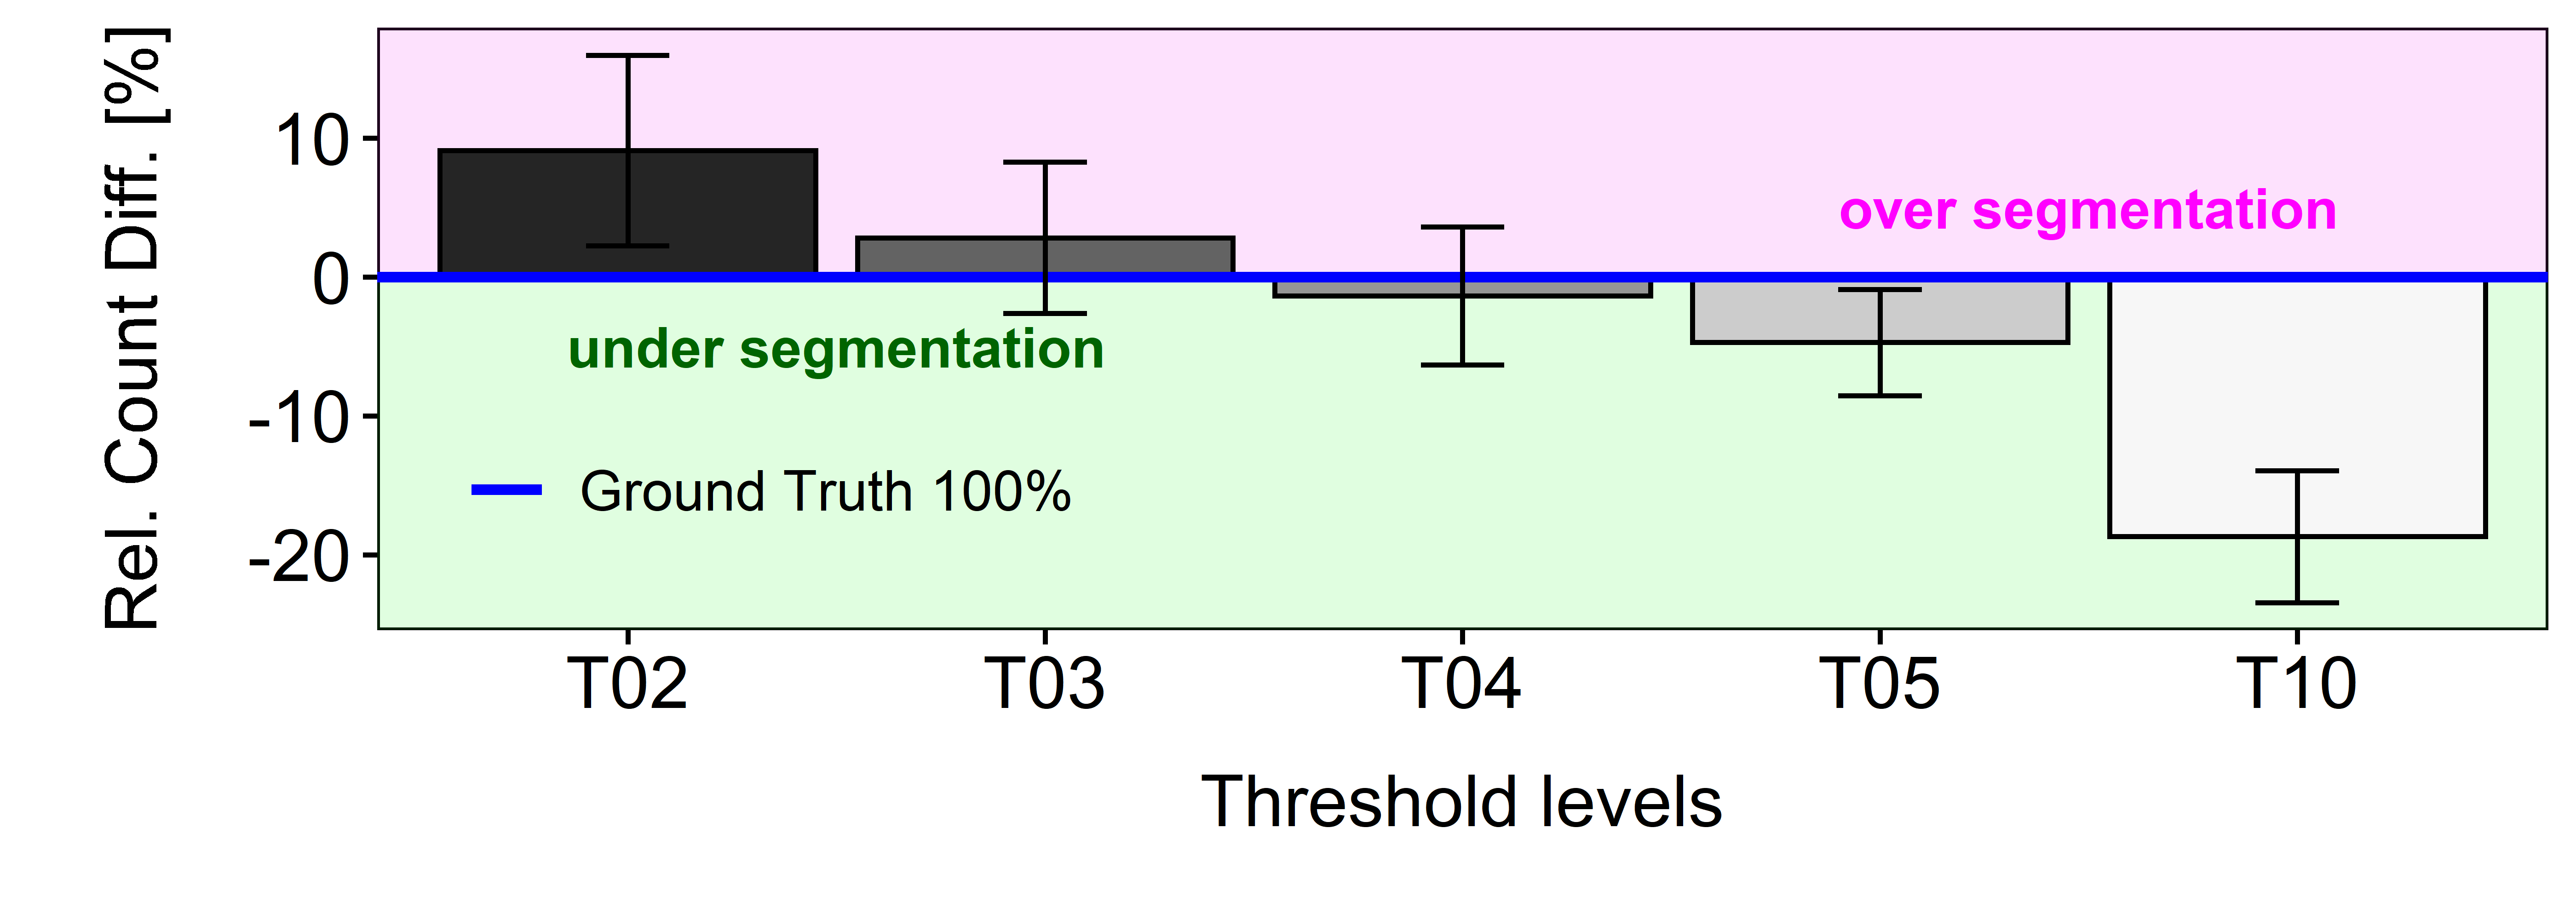
\includegraphics[width=0.65\linewidth]{thesis_dsk_files/figure-latex/gtratio-1} 

}

\caption[Relative difference of segment counts]{Relative difference of segment counts}\label{fig:gtratio}
\end{figure}
\hypertarget{apical-constriction-2}{%
\paragraph{Apical Constriction}\label{apical-constriction-2}}

For a proof of concept of segmentation results and concept around measuring Apical Constriction Index, analog to Harding(2013)(\emph{62}), 13 DMSO and 15 SU5402 treated embryos were imaged, segmented and processed. The results show a strong significant difference between DMSO und SU5402 treated embryos in both A.I.\textsubscript{Major} and A.I.\textsubscript{Minor}, validating the general concept.


\begin{figure}

{\centering 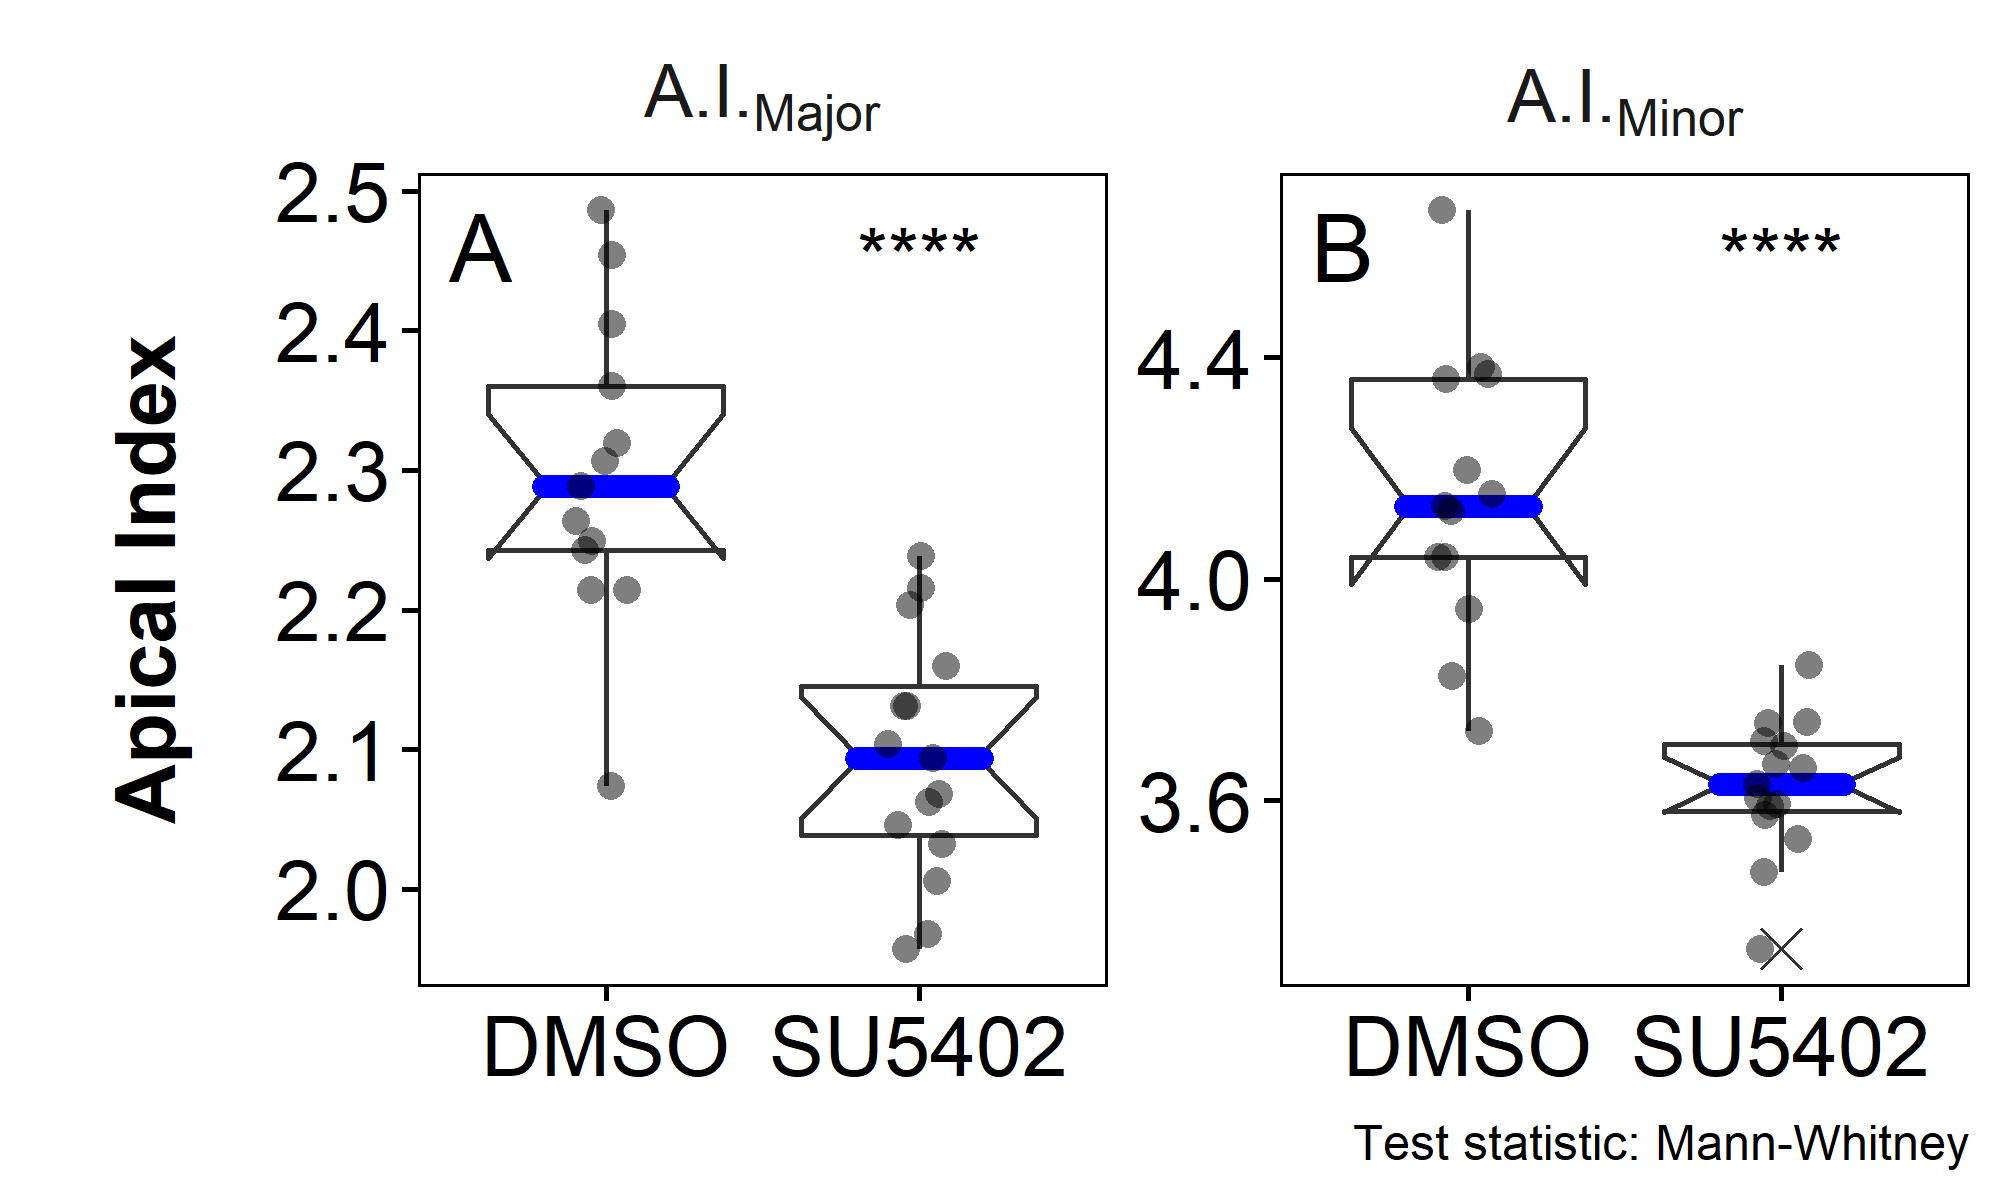
\includegraphics[width=0.5\linewidth]{thesis_dsk_files/figure-latex/resacimeasure-1} 

}

\caption[A.I. Major / Minor proof of concept]{A.I.\textsubscript{Major / Minor} proof of concept. \textbf{A and B} Each dot represents the average of all cells of a whole pLLP (DMSO = 1769 cells / 13 pLLPs; SU5402 = 2066 cells / 15 pLLPs).}\label{fig:resacimeasure}
\end{figure}
\hypertarget{cell-morphology}{%
\paragraph{Cell Morphology}\label{cell-morphology}}
\begin{quote}
\emph{There is always a precision / recall trade-off in detection tasks, e.g., when we set a lower threshold {[}. . .{]}, we can get a higher recall with a lower precision ({[}. . .{]}, but meanwhile we also get more false-positives in the results).}(\emph{51})
\end{quote}
Inspecting the cell count unfortunately does not directly tell us how well the cell morphology is conserved at different threshold levels, since at higher threshold levels the cell boundaries are differently determined and eventually not even recognized as such anymore. The volume of a cell is a very robust morphological feature with respect to changes in pose and topology (\emph{19}). Therefore, if its volume does not differ significantly at a given threshold level we consider its morphology to be conserved.

In figure \ref{fig:volsecdffull} the cell volumes and their distribution across the different threshold levels can be inspected. The closer the slopes are to the Ground Truth, the stronger they are conserved. The upper graph of figure \ref{fig:volsecdffull} shows the full distribution, where the major differences seem to appear within the 0.4 quantile (red line). To get a more detailed impression, in the lower graph of figure \ref{fig:volsecdffull} only the values \emph{within} the 0.4 quantile are shown.


\begin{figure}

{\centering 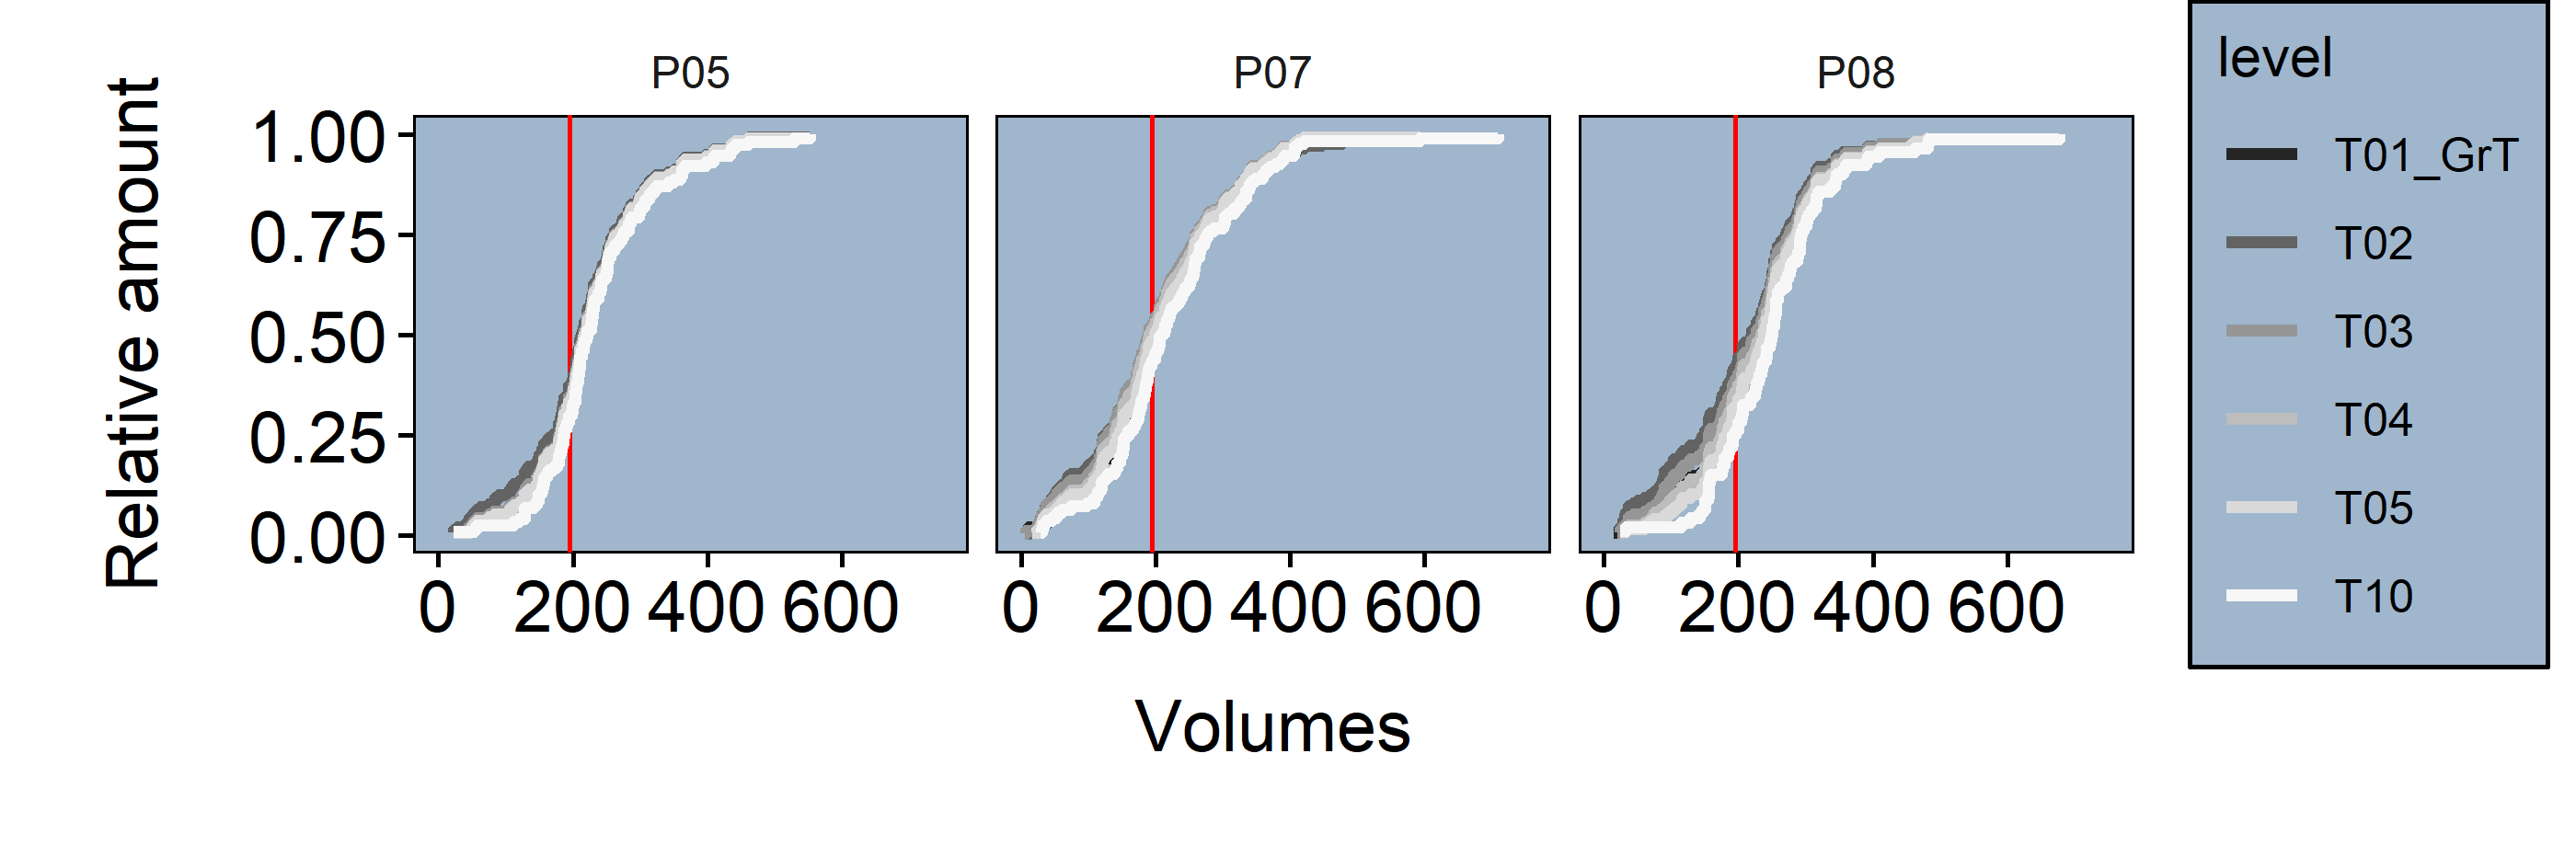
\includegraphics[width=0.9\linewidth]{thesis_dsk_files/figure-latex/volsecdffull-1} 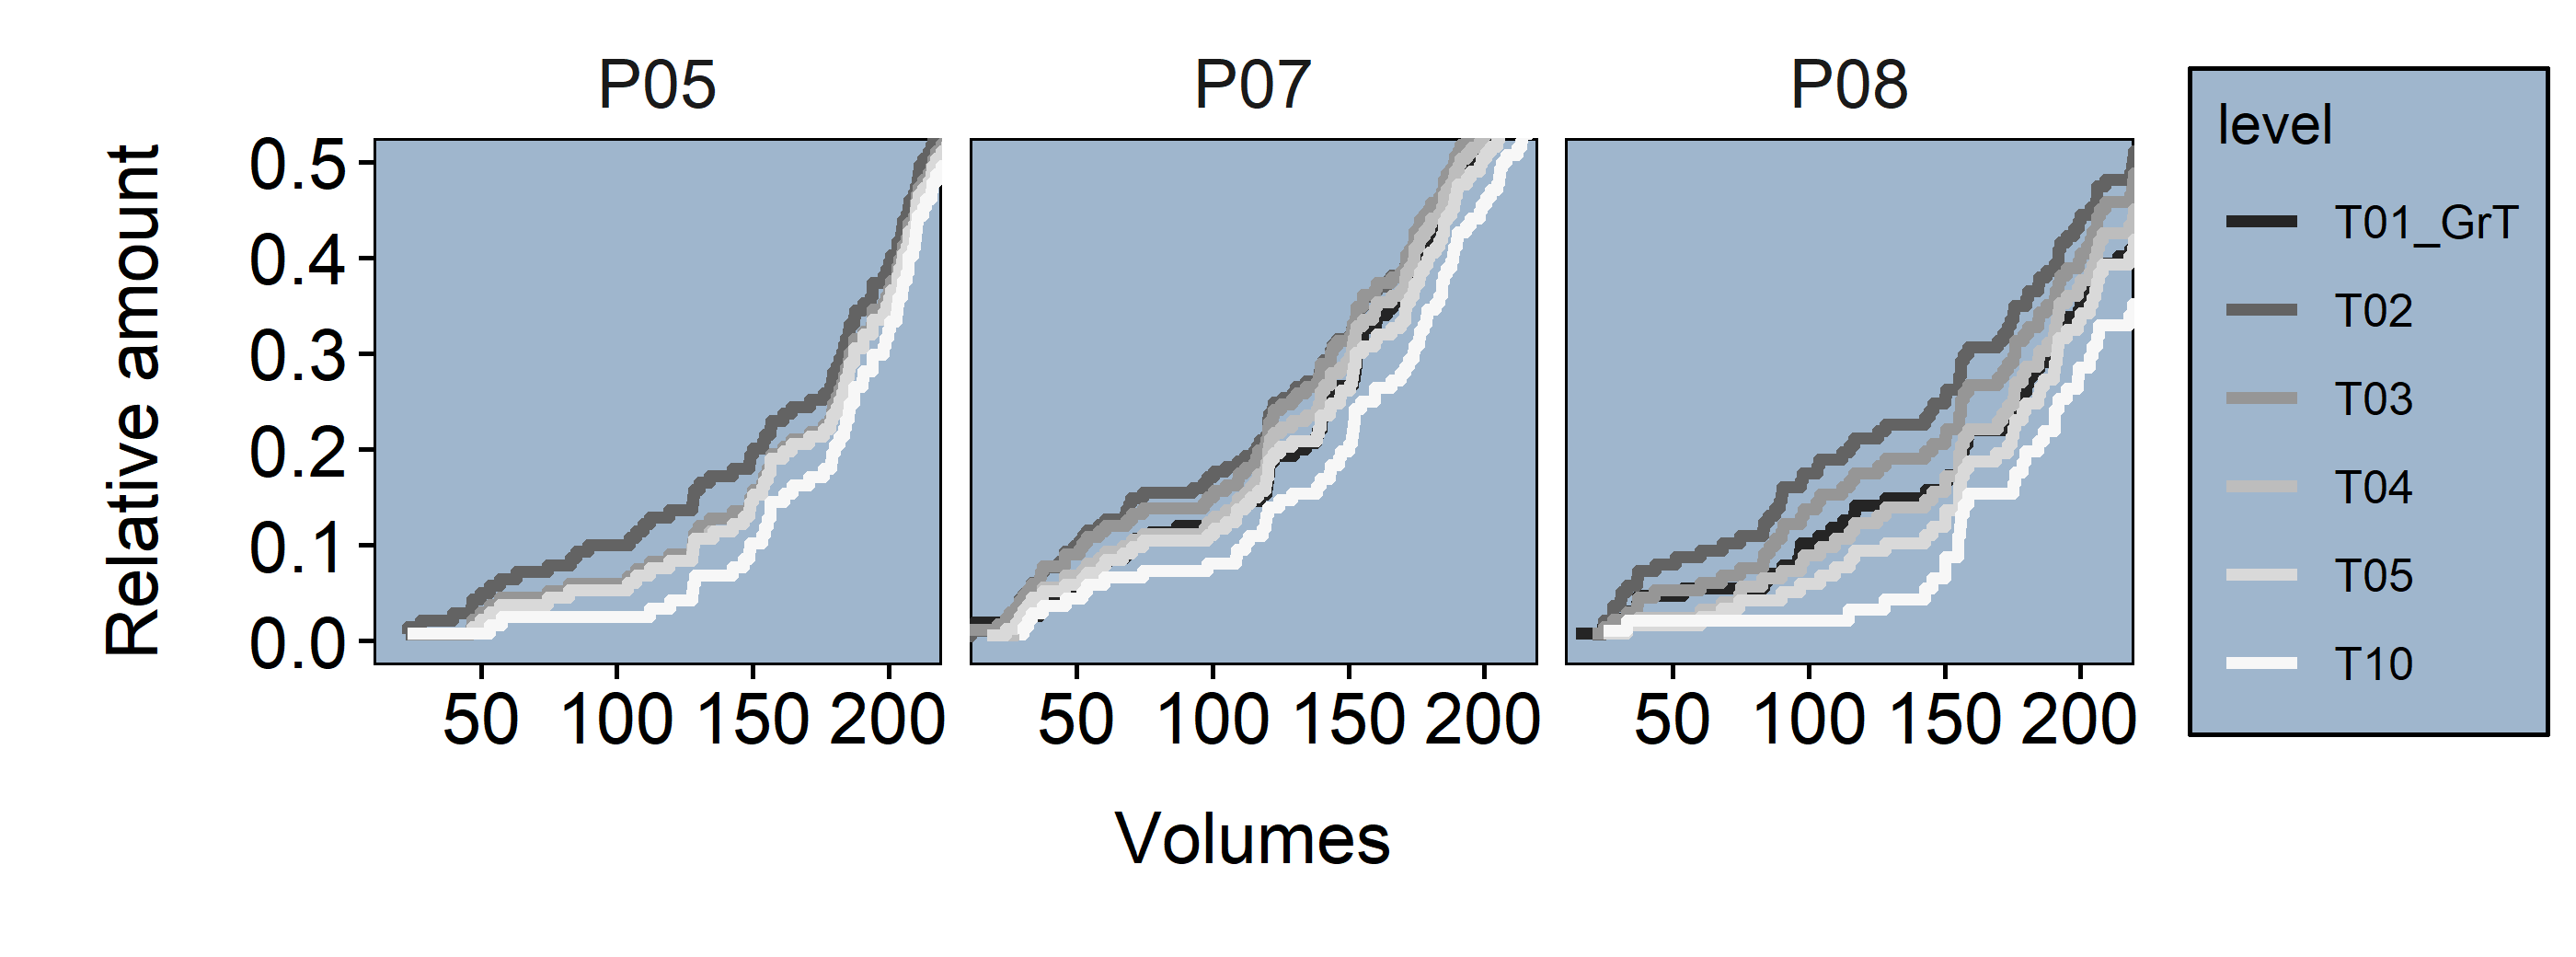
\includegraphics[width=0.9\linewidth]{thesis_dsk_files/figure-latex/volsecdffull-2} 

}

\caption[pLLP segmentation: morphological conservation]{\textbf{upper} Cell volumes full distribution (red line = .4 Quantile) \textbf{lower} Cell volumes distribution within .4 Quantile}\label{fig:volsecdffull}
\end{figure}
\hypertarget{confidence-level}{%
\paragraph{Confidence Level}\label{confidence-level}}

To statistically check how closely related each threshold level sample distribution is compared to the Ground Truth, a Kolmogorov-Smirnov-Test (ks.test) was performed. The ks.test is a nonparametric test whose null hypothesis is that the both groups compared were sampled from populations with identical populations. Therefore, the closer the p-value is to 1, the more similar the tested sample distribution would be to the Ground Truth (figure \ref{fig:kstestvol}).


\begin{figure}[H]

{\centering 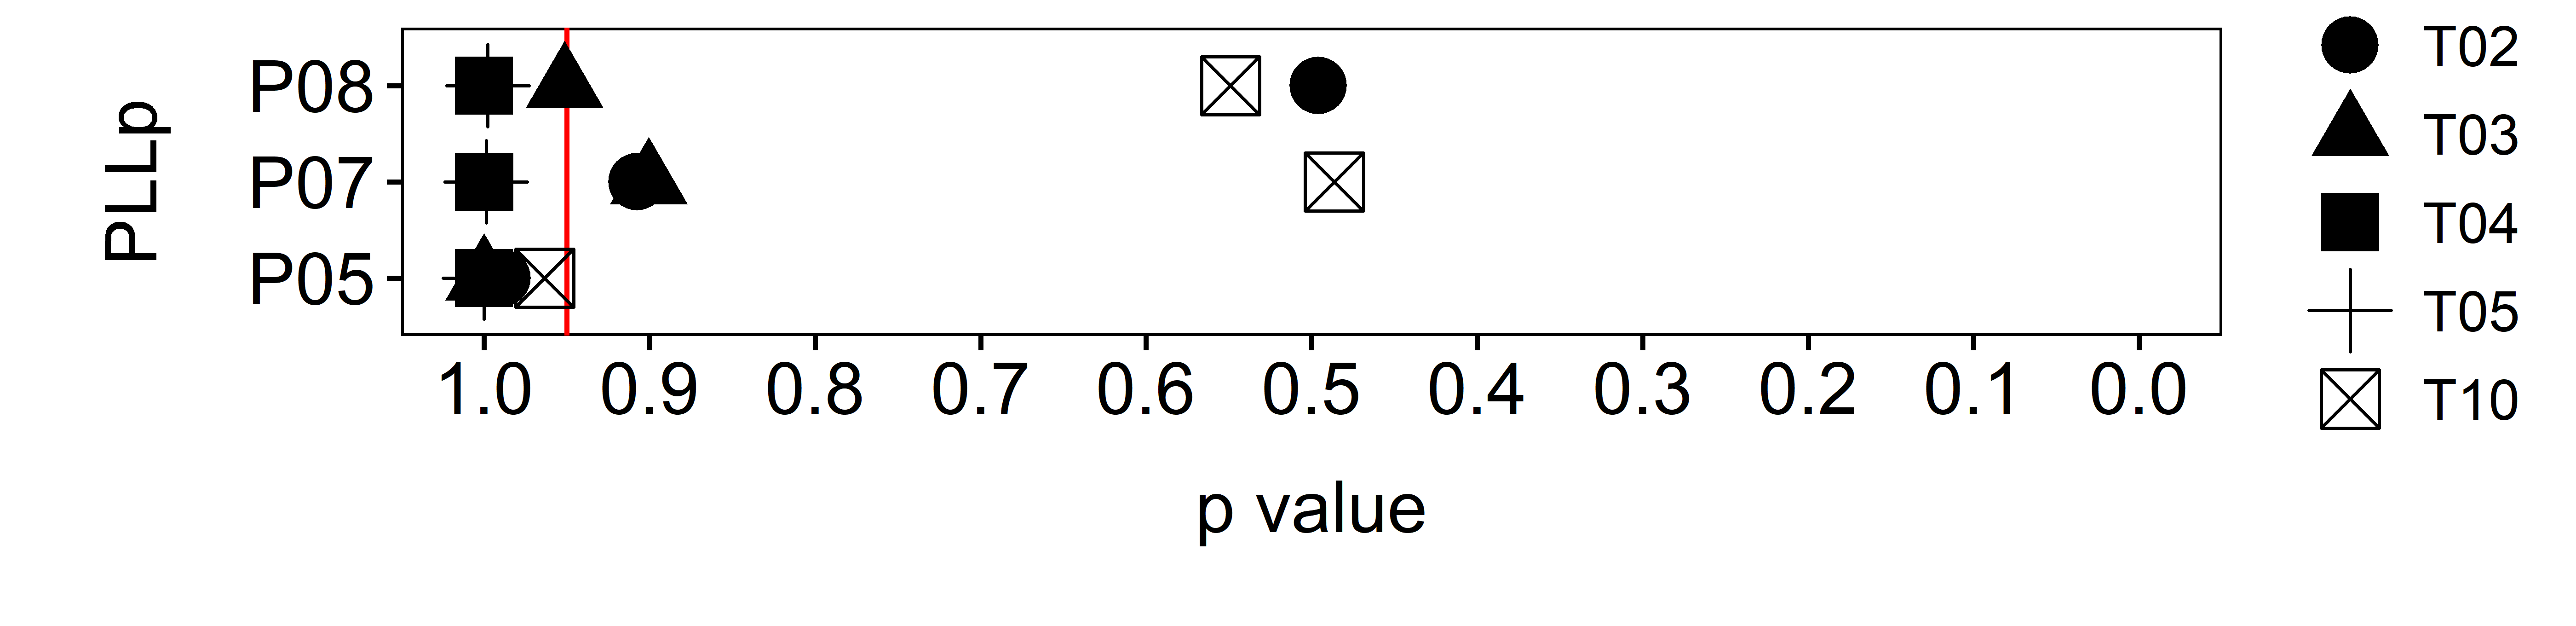
\includegraphics[width=0.7\linewidth,]{thesis_dsk_files/figure-latex/kstestvol-1} 

}

\caption{Volumetric conservation (red line = 5\(\%\))}\label{fig:kstestvol}
\end{figure}
\noindent In comparison to the Mann-Whitney test, the ks.test is more sensitive to detect changes in the shape of the distribution than to detect a shift of the median(\emph{71}). Since we have no reason to assume a significant change in the \emph{average} cell volume, it would not make much sense to use a test that requires averages. Instead we want to test if there is a change in the shape or skew of the whole distribution, which allows to compare each group on the single cell level (figure \ref{fig:volsecdffull}. In summary, the test results suggest a larger deviance in shape of distribution between the Ground Truth and the automatically segmented cells for Threshold levels T02 and T10. For T03 we are already close to rejection of the \(H_0\) hypothesis (assuming a 5\(\%\) threshold). Only for T04 and T05 are are well within the 5\(\%\) rejection threshold. However, since we want to be as close to the Ground Truth as possible, we settled for T04.

\hypertarget{CNN}{%
\subsection{Rosette Detection}\label{CNN}}

The method used for rosette detection is based on a convolutional neuronal network (CNN) and was modified from the ``rosette detector'' algorithm previously used in the lab and described in (\emph{1}, \emph{51}). Since the former method was technically outdated and since we had new data in which we needed to detect rosettes, we updated the former method to a \emph{state-of-the-art} CNN using Caffe(\emph{72}) as a backend. Network configuration and training was done by our collaborators at the institute for Informatics, Albert-Ludwigs-University Freiburg.

The training dataset consitsts of 17 DMSO- and SU5402- treated embryos each. SU5402 is an inhibitor of FGF receptors and embryos treated with these inhibitors show a strongly reduced number of rosettes (\emph{38}). In order to give the network something to learn, the data had to be labeled manually, which was done in ImageJ by placing multipoint ROIs at the center of the rosettes. The data was then further permutated (rotated and changed in size) to artificially increase the amount of training data and make the detection more robust against different kinds of input. Further parameters about the training data is listed in Table \ref{tab:cnntraintab}. One example for each is shown in figure \ref{fig:cnntrain}.


\begin{figure}

{\centering 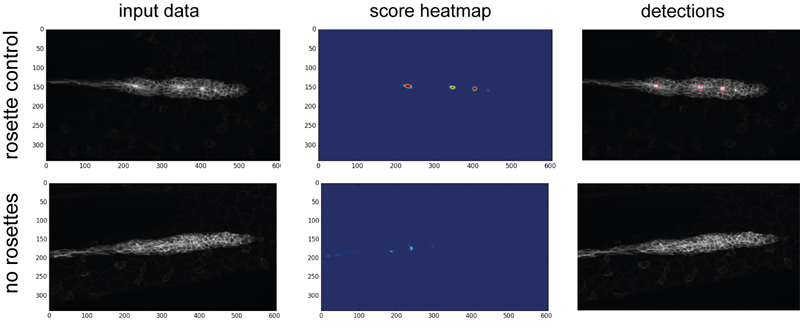
\includegraphics[width=0.75\linewidth]{figures/materials/cnn/CNNtrain} 

}

\caption[Example for rosette detection on the training data]{Example for rosette detection on the training data. \textbf{left} Maximum Z-projected input data. \textbf{middle} heatmap of scores. blue indicates a low score, red a high one. \textbf{right} score map projected onto the input data.}\label{fig:cnntrain}
\end{figure}
\noindent The main advantages for using a neural network in a task like this are\ldots{}
\begin{enumerate}
\def\labelenumi{\arabic{enumi}.}
\tightlist
\item
  Objectivity
  \begin{itemize}
  \tightlist
  \item
    A computer model is not biased in a way that it prefers one outcome over the other. It evaluates based on what it was trained to.
  \item
    Unlike the human brain, once a CNN is trained it is static and does not keep on learning. This promotes reproducibility.
  \end{itemize}
\item
  Degree of rosette registration
  \begin{itemize}
  \tightlist
  \item
    The output data are continuous rational numbers (\(\mathbb{Q}\)) instead of integers (\(\mathbb{Z}\)) which does not only tell if a rosette is there or not, but also for `how much' (50-100\(\%\)) it is there.
  \end{itemize}
\item
  Training is done relatively quick
\end{enumerate}
\begin{table}[!h]

\caption{\label{tab:cnntraintab}CNN training data}
\centering
\begin{tabu} to \linewidth {>{\centering}X>{\centering\arraybackslash}p{1cm}>{\centering\arraybackslash}p{2cm}>{\centering\arraybackslash}p{1.6cm}>{\centering\arraybackslash}p{1.5cm}>{\centering\arraybackslash}p{1.4cm}>{\centering}X}
\toprule
\textbf{group} & \textbf{conc.} & \textbf{nm} & \textbf{intensity....} & \textbf{exposure} & \textbf{z.planes} & \textbf{magnification}\\
\midrule
\rowcolor{gray!6}  DMSO & 0.1$\%$ & 488 & 100 & 100 ms & ~70 & 40X\\
SU5402 & 10$\mu$M & 488 & 100 & 100 ms & ~70 & 40X\\
\bottomrule
\end{tabu}
\end{table}
\hypertarget{shroom3}{%
\section{Shroom3}\label{shroom3}}

In the previous section a number of methods were presented I developed specifically to perform the analyses on the \emph{shroom3} mutant phenotype which are described in the following section.

\hypertarget{intro-phen}{%
\subsection{Phenotype description}\label{intro-phen}}

While birth rates follow a distribution of Mendelian inheritance (after genotyping at 3 months of age), mutant adults seem to be more sensitive to mechanical stress and have a shortened lifespan (\textasciitilde6-9 months). In body shape, \emph{shroom3} mutants are not smaller or possess any other striking phenotype (figure \ref{fig:shrmmut}C), however their gill flaps seem to be increased in size, swollen, and not exactly streamlined with the body. This is also evident by an increased frequency of gill flap beating. When looking at the pLLP at different stages (figure \ref{fig:shrmmut}D), they exhibit the same phenotype as the MO injected embryos (\emph{1}).


\begin{figure}

{\centering \includegraphics[width=0.95\linewidth]{figures/intro/shrm_mutants} 

}

\caption[shroom3 mutant phenotype]{\emph{shroom3} mutant phenotype \textbf{(A-A')} mutation strategy (A) Talen arms (black blocks) bordering a sequence within SD1 including a restriction site for NsiI (indicated back arrows and grey background) (A') wildtype and mutant allele with 8 bp deletion \textbf{(B-B')} Amino acid code and protein schematic with functional domains and stop codon (indicated by asterisk) \textbf{(C-C')} Adult phenotype with closeup to gill flaps \textbf{(D)} pLLP phenotype for three different stages (columns) and different manifestations (rows) (40X WI objective). Arrows indicate epithelial rosettes. \textbf{(E)} LL phenotype at end of migration (10X air objective). Scale bars = 1 mm. MaxIPs for D-E.}\label{fig:shrmmut}
\end{figure}
\emph{Shroom3} heterozygous zebrafish show no phenotypic abnormality. When incrossed, genotyping of two to five days post fertilization (dpf) embryos results in a Mendelian distribution. However, stock-fish that are regenerated and genotyped by finclip at about 3 months of age show only a rate of 5-10 \(\%\) of \emph{shroom3} homozygous mutants. After another 3 -- 6 months those would usually decease too. Therefore, the loss of Shroom3 activity leads to increased mortality for reasons we have not uncovered yet.

\hypertarget{lateral-line-morphometrics}{%
\subsection{Lateral Line Morphometrics}\label{lateral-line-morphometrics}}

Since in the previous study performed on \emph{shroom3} morphants we found a significantly reduced number of rosettes in the pLLP, a reduced number of CCs was expected to be deposited at the end of pLLP migration as well. Instead we found more CCs deposited \ref{fig:shrmmut}E.

\hypertarget{dataset}{%
\subsubsection{Dataset}\label{dataset}}

To analyze this observation quantitatively a dataset was put together consisting of 83 zebrafish embryos fixed at the end of pLLP migration, derived from four different parent pairs. After genotyping, this gave us 26 wildtypes, 31 heterozygous and 26 homozygous mutants for statistical tests. In addition to the number and position of deposited NMs, we also measured the area and the number of nuclei in each deposited CC.

\hypertarget{res-ccounts}{%
\subsubsection{Number and Position of Cell Clusters}\label{res-ccounts}}

Although the embryos were closely staged (\(\pm\) 20 min.), there are always some individual variations in the distance migrated by the pLLP of each. To compare the number of deposited CCs independently of LL length the ratio of LL length over CC count (\ref{fig:llcounts}B) was calculated. Fixation with PFA may introduce a slight bending of the embryo and mounting introduces a different tilt for each embryo, to correct for uneven LL paths and irregularities in mounting, CC distances are calculated in Euclidean space rather than solely in dimension X.

While \emph{shroom3}\(^{+/+}\) embryos deposit 6 \(\pm\) 0.7 CCs, \emph{shroom3}\(^{-/-}\) embryos deposit 8 \(\pm\) 0.9 CCs (figure \ref{fig:llcounts}A). This difference stays true also when normalizing against length (figure \ref{fig:llcounts}B).


\begin{figure}

{\centering 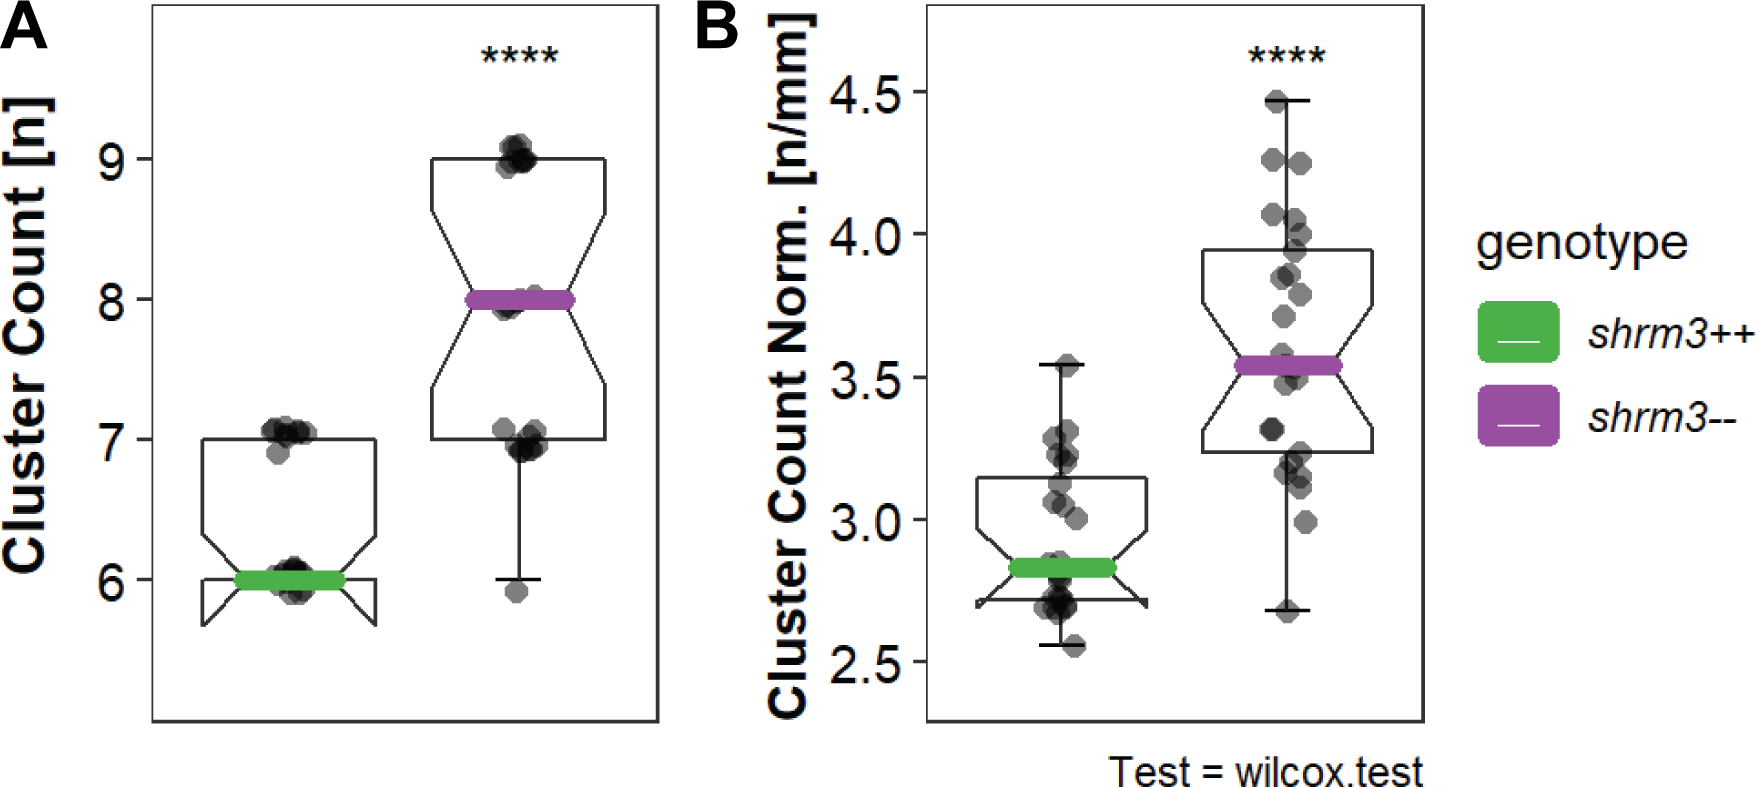
\includegraphics[width=0.6\linewidth]{figures/results/01_morphometrics/ll_counts} 

}

\caption[Cluster Counts]{Cluster counts. \textbf{A} cluster count {[}\(n\){]} \textbf{B} normalized to length (LL length {[}\(mm\){]} / cluster count {[}\(n\){]})}\label{fig:llcounts}
\end{figure}
Even though CC position in individual \emph{shroom3}\(^{-/-}\) embryos seems more random, the position of the first deposited CC is mostly conserved (\ref{fig:llpos}A), \(p\) for difference in position = 0.2). Similarly, the position of the pLLP isn't significantly changed confirming that Shroom3 activity is not required for migration, as was already shown in \emph{shroom3} morphants (\emph{1}). While for the remaining CCs an average lag of -50.4 \(\mu\)m as compared to \emph{shroom3}\(^{+/+}\) CC positions is observed, it also seems to increase with later CC positions. For \emph{shroom3}\(^{+/+}\) embryos CC position is mostly conserved through development, however it remains elusive if this is true for \emph{shroom3}\(^{-/-}\) embryos too.
Figure \ref{fig:llpos}A', shows the kernel density distribution for the CC position without grouping individual positions. At a binwidth of 50 \(\mu\)m, the distribution curves show a high and narrow density at around 350 \(\mu\)m, which is the average location of CC1 (\ref{fig:llpos} 2A). For the remaining CCs the kernel distribution does, neither for \emph{shroom3}\(^{+/+}\) nor for \emph{shroom3}\(^{-/-}\) embryos, reveal a precise location. In contrast, if based on CC sequential identity the mean position and standard deviation is calculated, a more explicit pattern emerges which clearly shows the increased count and average frequency (\ref{fig:llpos} 2A).

This shows that in the absence of Shroom3 activity, more NMs form. This is particularly surprising since the lab had previously shown that \emph{shroom3} knock-down leads to a defect in rosette formation and these rosettes prefigure the deposited NM.


\begin{figure}

{\centering 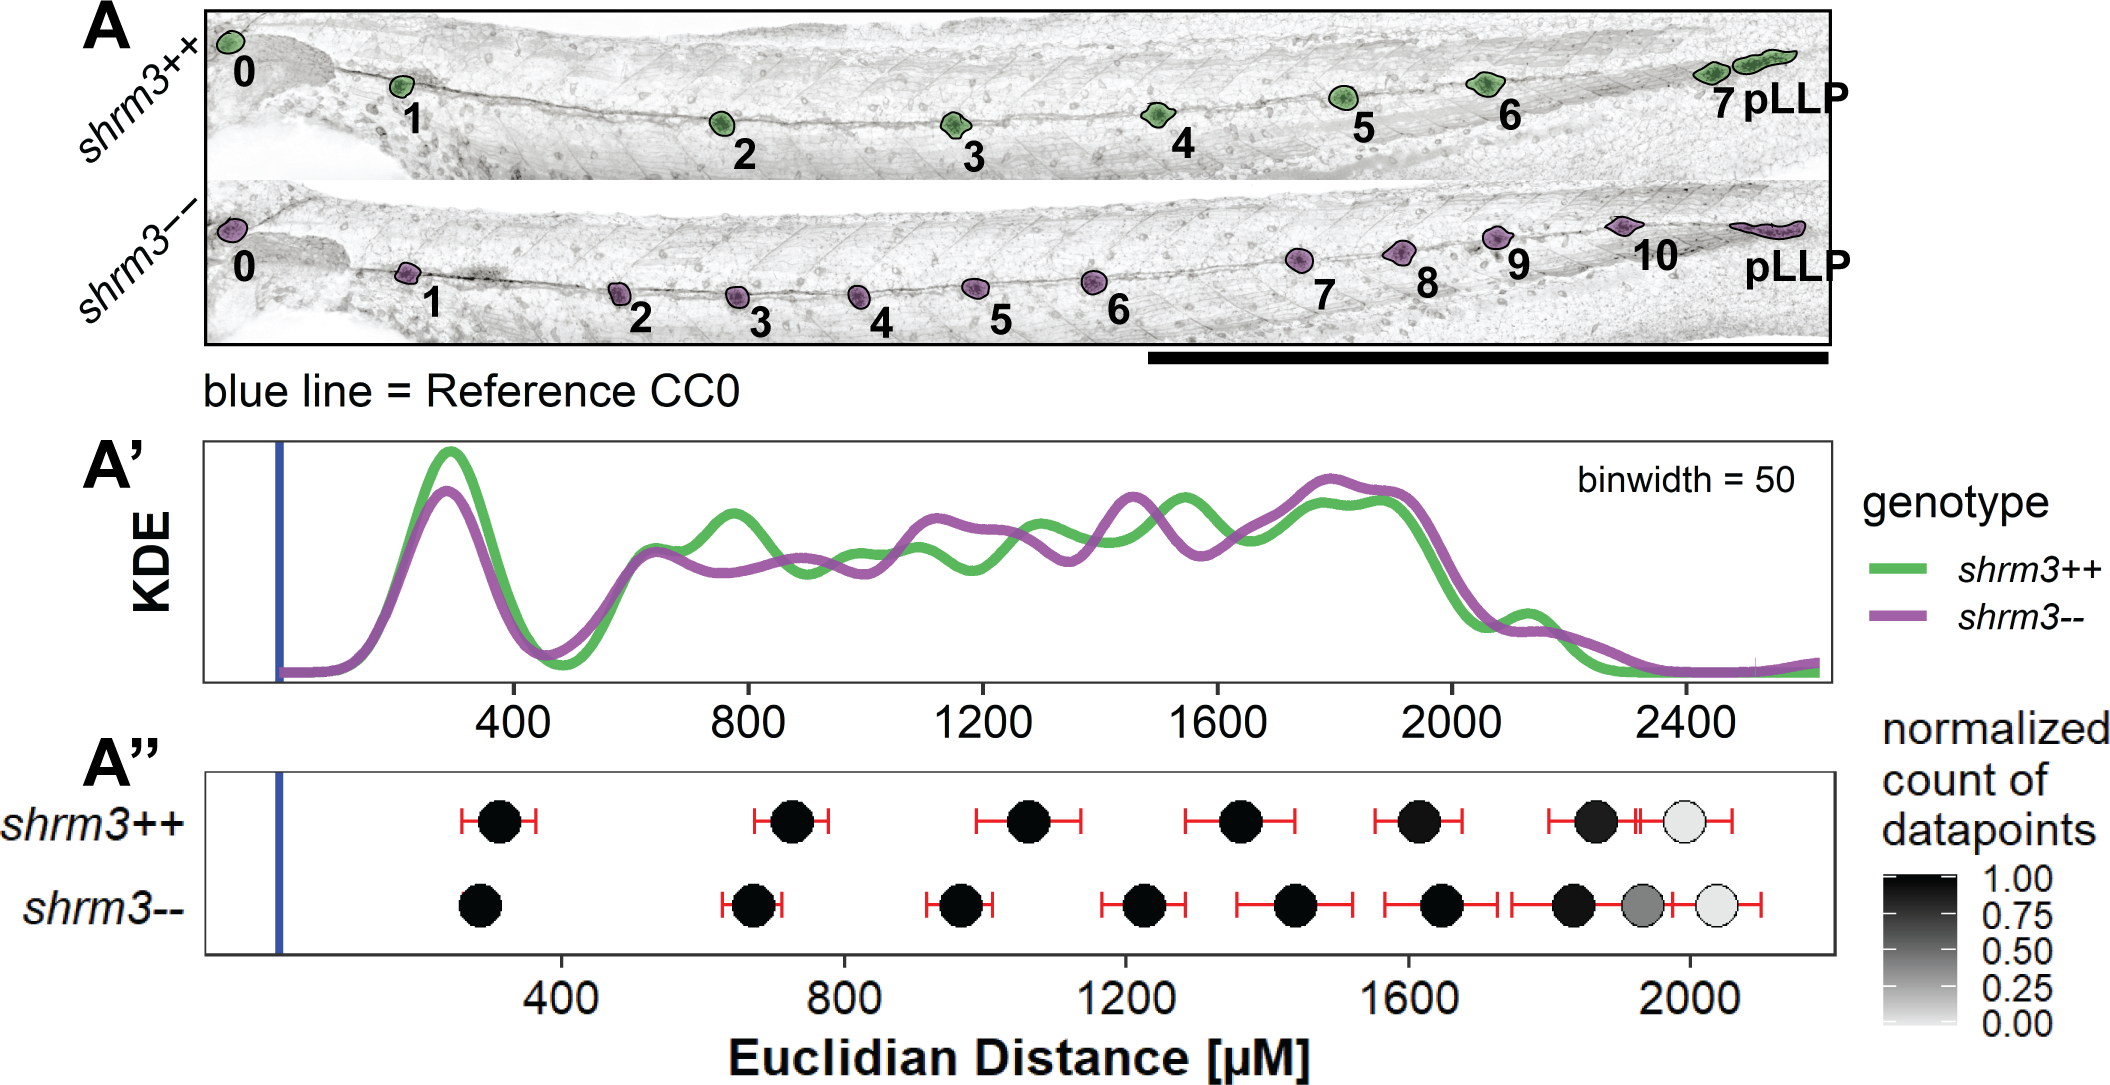
\includegraphics[width=0.85\linewidth]{figures/results/01_morphometrics/ll_positions} 

}

\caption[Cell Cluster Positions]{Cell Cluster positions. \textbf{A} Exemplary \emph{shroom3}\(^{+/+}\) and -\/- embryos with CCs highlighted. CC0 marks the reference location to compare individual embryos. Scale bar = 1 mm \textbf{A'} Kernel Density Estimate without (KDE) grouping (\(n\)++ = 162, \(n\)-\/- = 206) \textbf{A''} Dots = mean positions, bars = standard deviation (\(n\)max for both ++ and -\/- = 26).}\label{fig:llpos}
\end{figure}
\hypertarget{res-llmorph}{%
\subsubsection{Cell Count and Area of CCs}\label{res-llmorph}}

The CC count and position analysis clearly shows that more CCs are deposited in \emph{shroom3} mutant embryos. In order to determine whether these additional clusters are comprised of as many cells as their wild-type counterparts or less, I quantified the number of cells and the size of each clusters in \emph{shroom3}\(^{-/-}\) embryos, the cell count per CC was determined by counting DAPI stained cells within CC segments derived from the \emph{cldnb:lyn-gfp} membrane signal (section \ref{mat-GrTrDat}). Both the CC cell number and the CC area were reduced by about 6\(\%\) in \emph{shroom3}\(^{-/-}\) embryos so that the density remains unchanged (\ref{fig:llclus}A). Interestingly, the total number of cells in CC per embryo is increased by 9\(\%\) (\ref{fig:llclus}B). Both the sum of CC cells and total LL cells (CC+pLLP) are significantly increased in \emph{shroom3}\(^{-/-}\) embryos, while the count of only pLLP cells remains unchanged.


\begin{figure}[H]

{\centering 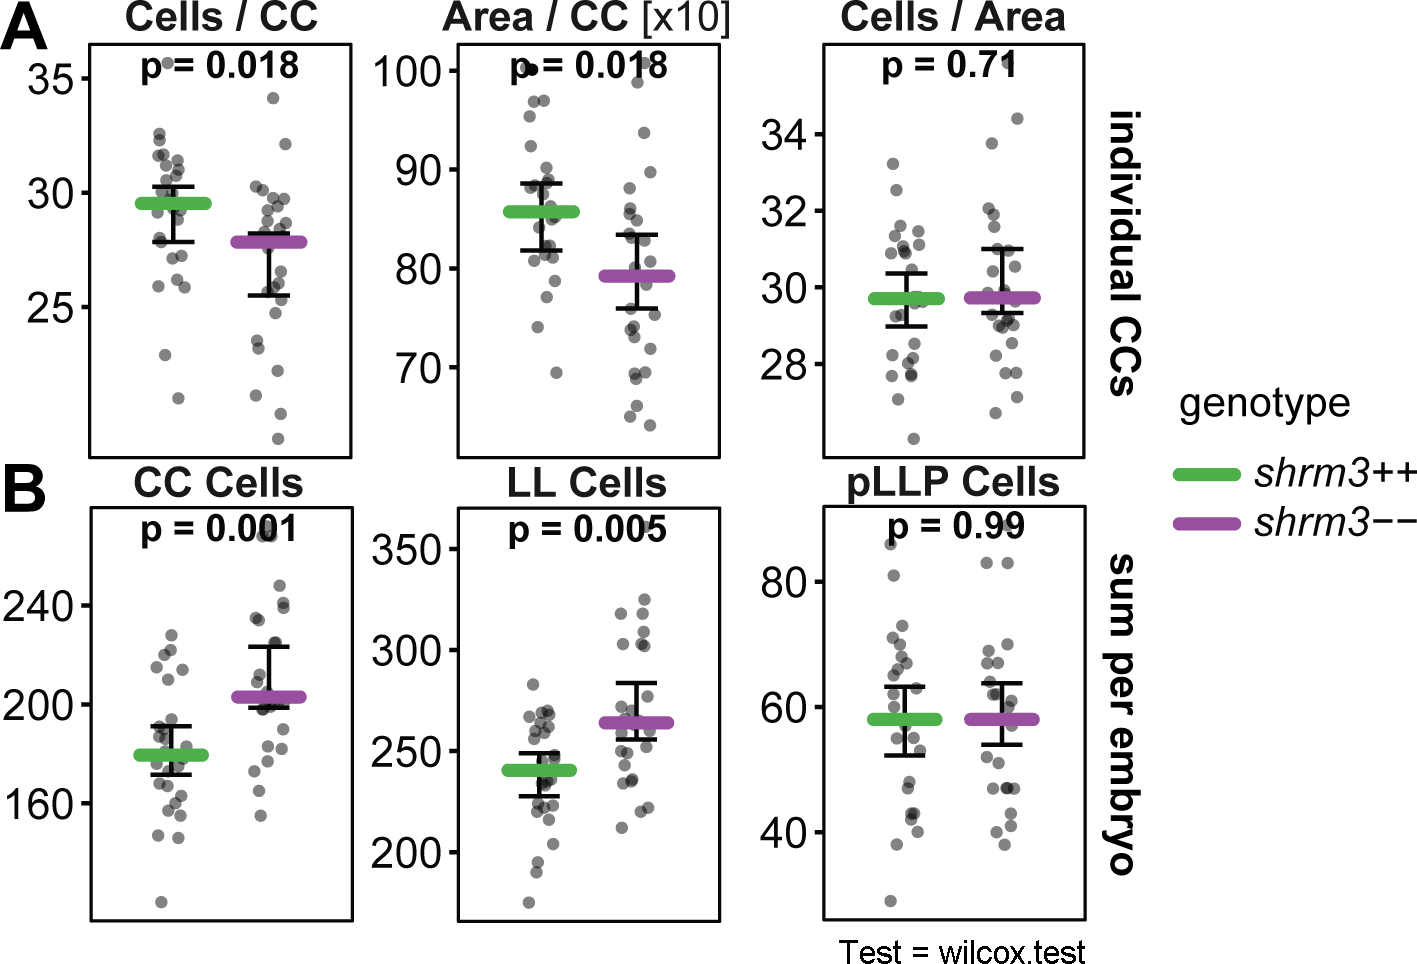
\includegraphics[width=0.65\linewidth]{figures/results/01_morphometrics/ll_clusters} 

}

\caption[LL Morphometrics]{LL Morphometrics \textbf{A} individual CC statistics \textbf{B} Sums per embryo. (Bars = median, errorbars = 95\% CI)}\label{fig:llclus}
\end{figure}
\hypertarget{res-tempresc}{%
\subsubsection{Temperature Rescue}\label{res-tempresc}}

Increasing temperature usually leads to an acceleration in thermodynamics and embryonic development, while lower temperatures slow down development (\emph{73}). Slowing down development also leads to a reduction in speed of migration and therefore to a reduction in forces that act on cells, cell-cell junctions and organ structures.

For this experiment the hypothesis to test was that it should be possible to at least partially restore the \emph{shroom3}\(^{+/+}\) number of CCs by giving rosettes a longer time to develop properly. Since embryos develop at different speeds, it is more challenging to exactly stage match them at end of migration. To account for this the CC count was normalized to LL length.


\begin{figure}[H]

{\centering 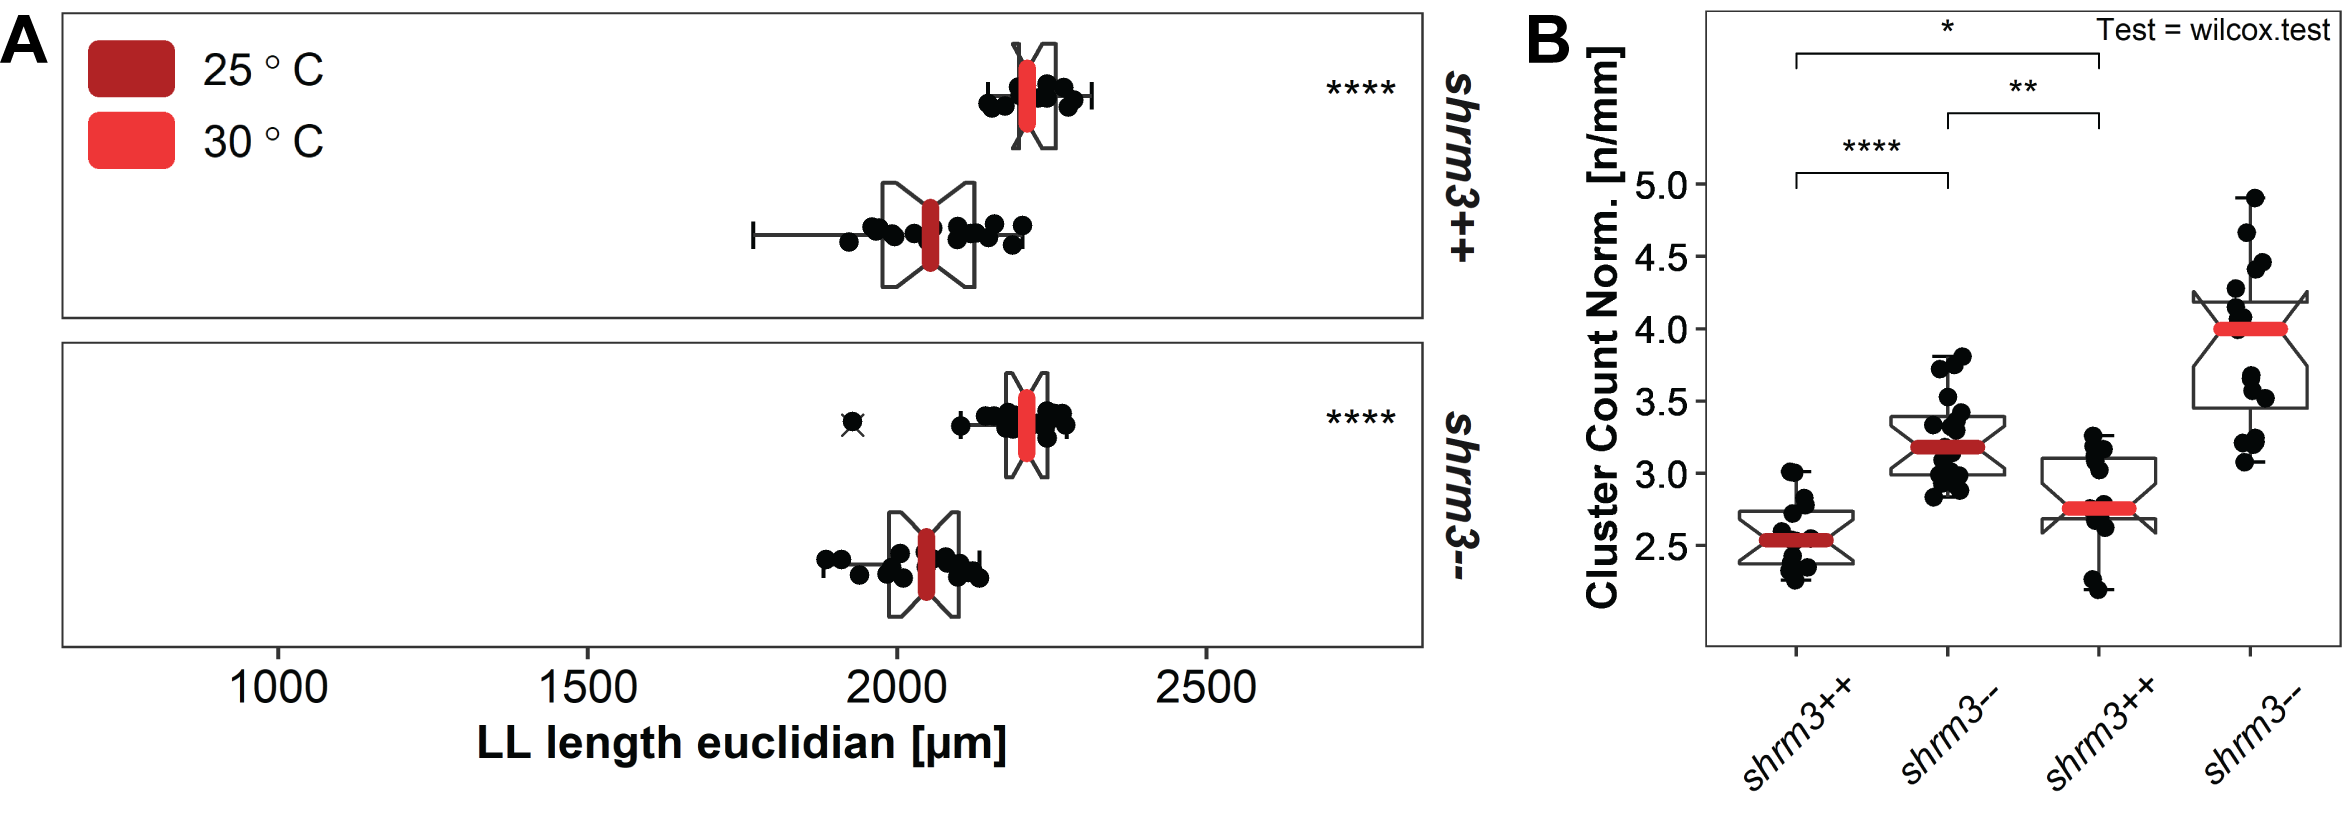
\includegraphics[width=0.85\linewidth,]{figures/results/06_rescues/temp/rescue_temp} 

}

\caption[Rescue: Thermodynamics]{Temperature rescue \textbf{A} LL lengths and end of migration stage matching \textbf{B} groupwise comparison of the length normalized CC count \emph{per} temperature.}\label{fig:resctemp}
\end{figure}
The question was if we could restore wildtype CC counts in \emph{shroom3}\(^{-/-}\) embryos when incubating at lower temperatures. Therefore, we need to compare CC counts between T25-\/- and T30++ resp. p-values between the pairs T30-\/- \emph{vs} for T30++ (the original) and T25-\/- \emph{vs} T30++ (the actual hypothesis). Even though the CC count T25-\/- cannot be completely restored (\textasciitilde3.2 to \textasciitilde2.8 in median normalized CC count), the difference between tested pairs shrunk from 0.00000 (T30-\/- \emph{vs} for T30++) to 0.00210 (T25-\/- \emph{vs} T30++), which is much closer to a rejection of \(H_0\). At this point, the question remains open but seems probable that at even lower temperatures the wildtype CC count could be rescues in \emph{shroom3}\(^{-/-}\) embryos.
\begin{table}

\caption{\label{tab:resctemptab}Temperature rescue dataset summary}
\centering
\begin{tabu} to \linewidth {>{\centering}X>{\centering}X>{}c|>{\centering}X>{\centering}X>{\centering}X}
\toprule
genotype & treatment & LLs & genotype & treatment & LLs\\
\midrule
 & 25°C & 18 &  & 25°C & 19\\

\multirow[t]{-2}{*}{\centering\arraybackslash \textit{shroom3}++} & 30°C & 15 & \multirow[t]{-2}{*}{\centering\arraybackslash \textit{shroom3}$--$} & 30°C & 20\\
\bottomrule
\end{tabu}
\end{table}
\begin{table}

\caption{\label{tab:resctempsignif}Temperature rescue statistics}
\centering
\fontsize{7}{9}\selectfont
\begin{tabu} to \linewidth {>{\raggedleft}X>{\raggedright}X>{\centering}X>{\centering}X>{\centering}X}
\toprule
group1 & group2 & p & p.adj & p.signif\\
\midrule
 & T25 $--$ & 0.00000 & 0.00000 & ****\\

 & T30 ++ & 0.00747 & 0.00750 & **\\

\multirow[t]{-3}{*}{\raggedleft\arraybackslash T25 ++} & T30 $--$ & 0.00000 & 0.00000 & ****\\

 & T30 ++ & 0.00104 & 0.00210 & **\\

\multirow[t]{-2}{*}{\raggedleft\arraybackslash T25 $--$} & T30 $--$ & 0.00015 & 0.00046 & ***\\

T30 ++ & T30 $--$ & 0.00000 & 0.00000 & ****\\
\bottomrule
\end{tabu}
\end{table}
\hypertarget{summary-2}{%
\subsubsection{Summary}\label{summary-2}}

Two additional CCs are deposited in \emph{shroom3}\(^{-/-}\) embryos. While each CC is comprised of less cells, in sum there are more cells in embryos deficient for Shroom3 leading to a net increase in cell count of \textasciitilde9\(\%\) (31 cells). Rescuing the CC count by slowing down embryonic development was only partially successful, but seems probable at even lower temperatures. For the pLLP at end of migration however, the number of cells is unaffected - which raises the question if Shroom3 has a regulatory role in Proliferation.

\hypertarget{proliferation}{%
\subsection{Proliferation}\label{proliferation}}

LL morphometric analysis revealed that deposited CCs in \emph{shroom3}\(^{-/-}\) embryos were on average slightly smaller and had fewer cells incorporated. However, due to the additional two cell clusters deposited, the net count is \textasciitilde9\(\%\) increased at the end of migration.
To test whether this is due to higher proliferative activity a dataset of time-lapse movies (12 h / \(\Delta\)T = 6 min.) was generated to count the number of mitoses in a \emph{cxcr4b(BAC):H2BRFP} transgenic background similar to previous proliferation studies in the pLLP (\emph{34}, \emph{74}).

\hypertarget{datasets}{%
\subsubsection{Datasets}\label{datasets}}

The live imaging dataset consists of 12 \emph{shrm3}++ and 18 \emph{shrm3}-\/- embryos with about 75 timepoints for each pLLP and 150 cell clusters. For counting, tracks were created for each proliferative cell on MaxIPs (section \ref{prolif}). Figure \ref{fig:prolpLLP}A shows a \emph{shroom3}\(^{+/+}\) and a \emph{shroom3}\(^{-/-}\) LL after 12 h of imaging where each mitotic track is individually colored and overlaid to the image data.

To support and validate this data two more datasets from fixed embryos were generated, one with a EdU (N = 3, n++ = 26, n-\/- = 17) and one with a phospho-Histone marker (N = 3, n++ = 22, n-\/- = 29).

\hypertarget{res-prolpLLP}{%
\subsubsection{Lateral Line Mitoses}\label{res-prolpLLP}}

Tracking mitoses in the pLLP does not reveal any difference in proliferation from start (\textasciitilde28 hpf) till about mid of migration 12 hours later (\ref{fig:prolpLLP}B). For confirmation, this finding was also validated \emph{via} two more additional methods. During the cell cycle genetic material is replicated in S-phase, while in metaphase of mitosis histones are found to be heavily phosphorylated (\emph{75}). With an 5-Ethynyl-2'-deoxyuridine (EdU) assay (\emph{76}), cells in S-phase can be detected (\ref{fig:prolpLLP}B'). Using a specific phospho-Histone (p-Hist.) antibody cells in meta-phase can be detected. When comparing the
EdU index (EdU positive cells over total pLLP cell number) or the mitotic index (p-Hist. positive cells over total pLLP cell number) I could confirm that there is no difference in proliferation in the migrating pLLP. Still, at the end of migration the LL system in \emph{shroom3}\(^{-/-}\) embryos does contain 9\(\%\) more cells (figure \ref{fig:llclus}).


\begin{figure}

{\centering 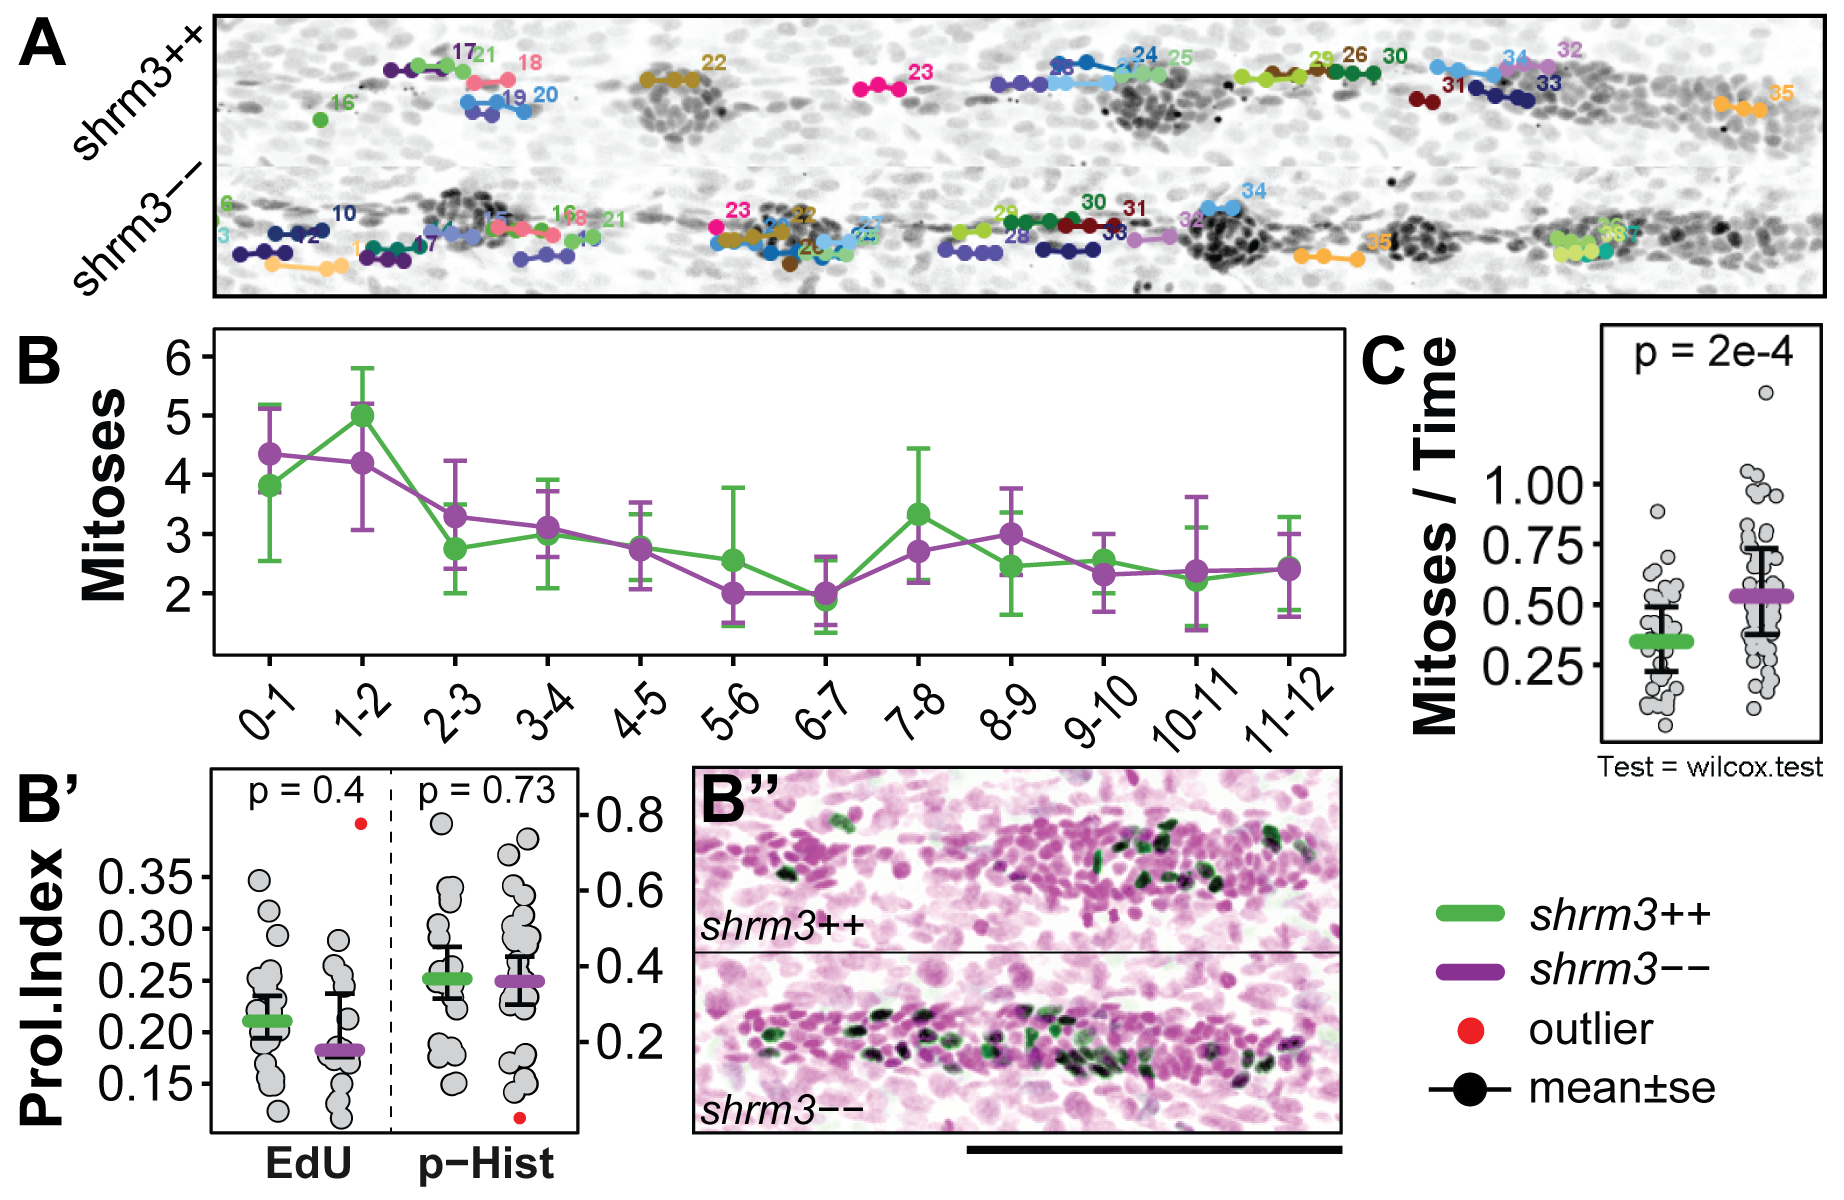
\includegraphics[width=0.85\linewidth]{figures/results/02_proliferation/prol-01} 

}

\caption[pLLP proliferation]{pLLP proliferation \textbf{A} Tracks of Mitosis. (Image data) Last timepoint of Z-projected time-lapse movie. (Labels) each dots marks a mitotic events. Each color represents one mitosis. Each connection between two dots represents 6 min. \textbf{B-B''} Mitoses in the pLLP. (B) Count of Mitoses through time (mean\(\pm\)sd) (B') Proliferation Index at 36 hpf for EdU and phospho Histone labeled pLLPs (B'`) Examples of EdU staining (scale bar = 100 \(\mu\)m) \textbf{C} Mitoses in CCs. B' and C, the colored bar indicated the median, bars indicate the 95\% CI.}\label{fig:prolpLLP}
\end{figure}
Since individual \emph{shroom3}\(^{-/-}\) CCs are smaller, we wondered if there could be compensation mechanisms activated that increases proliferation to restore wildtype CC size once they are deposited. To verify this, CC mitoses were tracked on the same data as before. Other than the pLLP, which can be observed throughout the time-lapse, CCs only begin to \emph{exist} when they are deposited. To normalize for individual CC lifetimes, the number of mitoses per CC is divided by the duration of the total time-lapse minus the time span to when it first appeared.
\begin{definition}[Normalized mitotic rate]
\protect\hypertarget{def:unnamed-chunk-10}{}{\label{def:unnamed-chunk-10} \iffalse (Normalized mitotic rate) \fi{} }\[\frac{mitoses\ per\ CC\ [n]}{total\ time- time\ of\ deposition\ [T]}\]
\end{definition}
This clearly shows that the additional cells in \emph{shroom3}\(^{-/-}\) embryos are derived from CC proliferation, rather than pLLP proliferation (\ref{fig:prolpLLP}C).

\hypertarget{summary-3}{%
\subsubsection{Summary}\label{summary-3}}

These results show that the additional cells at the end of migration observed in the LL analysis do not stem from an increase in proliferation in the pLLP, but instead from increased proliferation after CCs are deposited.

\hypertarget{rosette-formation-and-cluster-deposition}{%
\subsection{Rosette Formation and Cluster Deposition}\label{rosette-formation-and-cluster-deposition}}

Having shown that the additional CC deposition in \emph{shroom3}\(^{-/-}\) embryos is not caused by an over-proliferation in the migrating pLLP, the next step was to have a closer look at the dynamics of rosette formation, in relation to pLLP morphometrics and CC deposition. To test dependencies between different observations and developmental dynamics, variables can be correlated. To do this and to have a coherent dataset to work with, the data of three different analyses on a single set of image data were joined.

\textbf{First}, to get to know the exact timing of CC deposition, a manual tracking tool (\emph{59}) was used (figure \ref{fig:rdt}, tracking). \textbf{Second}, to deduce pLLP morphometrics an IJ macro was developed (anaLLzr2DT, section \ref{mat-anallzr2dt}) for spatiotemporal registration of the pLLP and to yield information about its speed, area, roundness, etc. (\ref{fig:rdt}, Registration). \textbf{Third}, to detect rosettes and quantify their weights, a CNN (\emph{77}) was used on the registered pLLP output from the before mentioned IJ macro (section \ref{CNN}; figure \ref{fig:rdt} - Detection).
Finally, all three datasets were joined by embryo id and timepoint.

\hypertarget{res-det-ds}{%
\subsubsection{Dataset}\label{res-det-ds}}

The image data set analyzed consists of 20 time-lapse movies (11 \emph{shroom3}\(^{-/-}\), 9 \emph{shroom3}\(^{+/+}\)). Each time-lapse has a duration of \textasciitilde20 h (\textasciitilde8 min. interval)\footnote{for further details about dataset acquisition see section \ref{mat-datasets} - Proliferation dataset}, summing up to \textasciitilde1650 \emph{shroom3}\(^{-/-}\), and \textasciitilde1350 \emph{shroom3}\(^{+/+}\) timepoints.


\begin{figure}[H]

{\centering 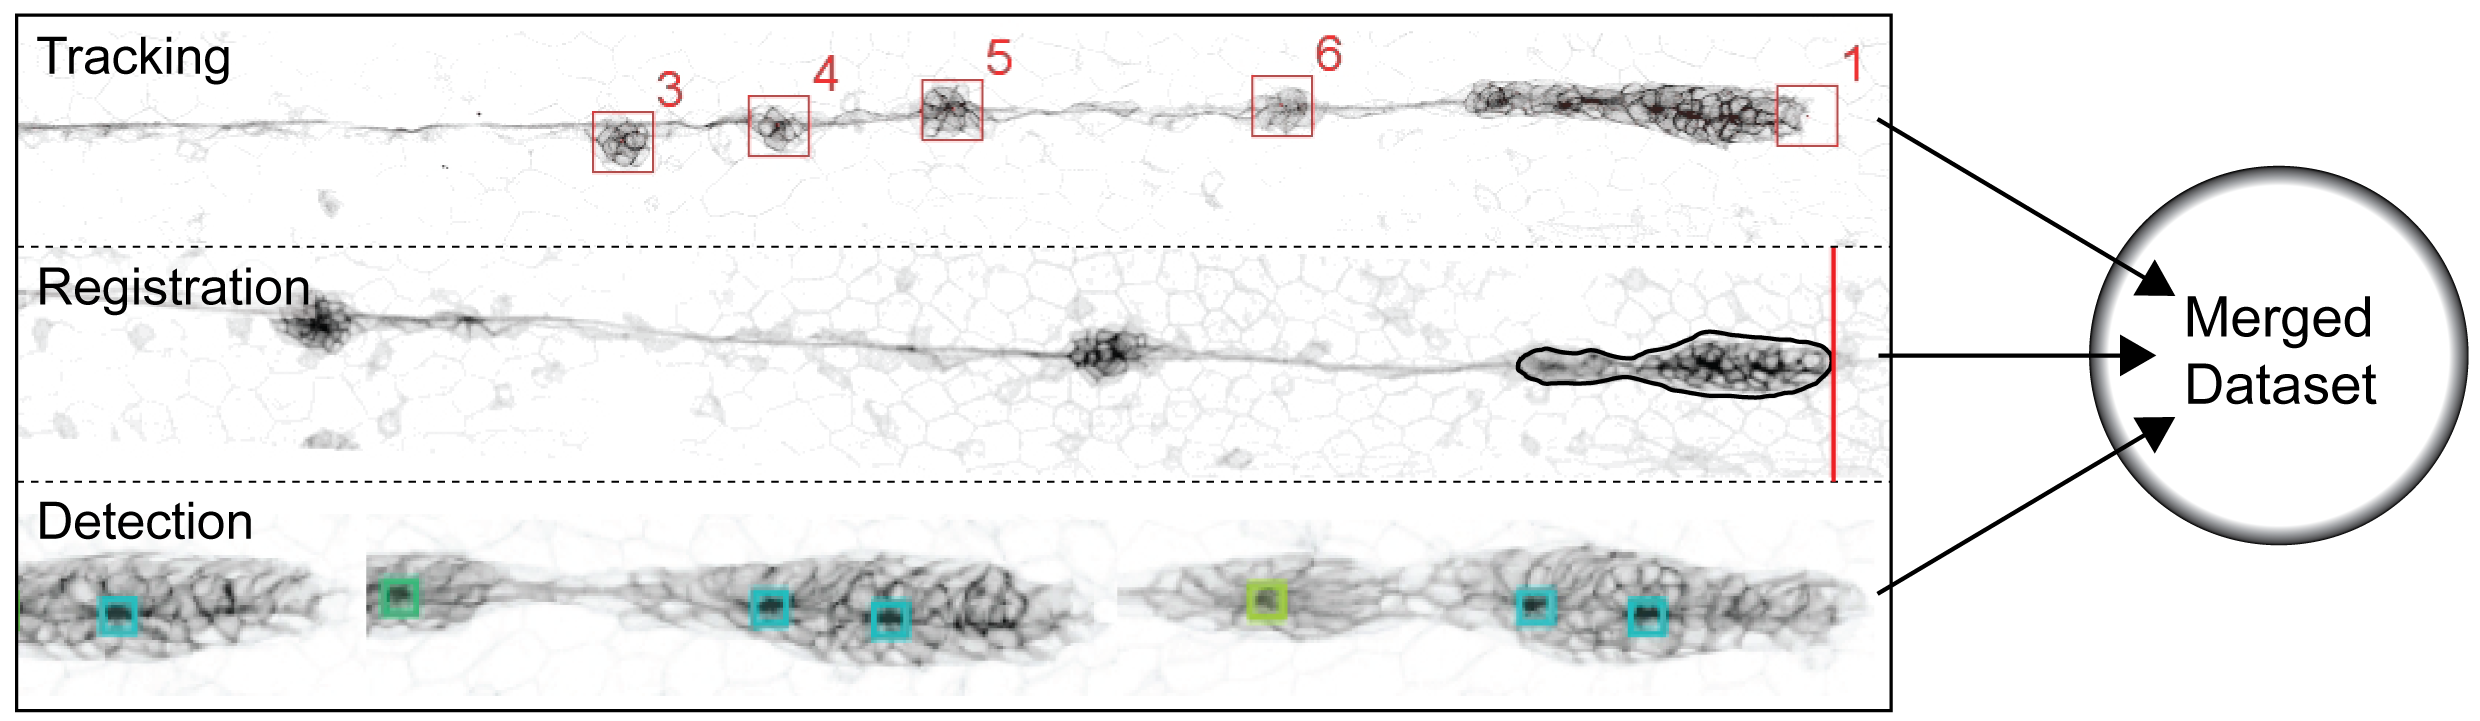
\includegraphics[width=0.85\linewidth]{figures/results/03_rosettes/RDT-01} 

}

\caption[Rosette Formation Joined Datasets]{Rosette Formation Joined Datasets. \textbf{Tracking} pLLP is marked as no.1. The rest of the CCs is numbered sequentially as they appear. \textbf{Registration} The black outline marks the region of interest (ROI) that is the pLLP as it is detected by the anaLLzr2DT. The red line highlights the pLLPs leading edge. \textbf{Detection} Each square highlights a detected rosette by the CNN, colors represent rosette weights.}\label{fig:rdt}
\end{figure}
\hypertarget{cluster-deposition}{%
\subsubsection{Cluster Deposition}\label{cluster-deposition}}

Figure \ref{fig:rdtdepo}A shows a montage of a \emph{shroom3}\(^{+/+}\) and a \emph{shroom3}\(^{-/-}\) scenario in cluster deposition (3.5 h / \textasciitilde20 min. interval). For \emph{shroom3}\(^{+/+}\) the rosette structure seems tight and two depositions occur in a regular manner. In the \emph{shroom3}\(^{-/-}\) on the other hand, rosette structure are more fragile with less pronounced rosette centers and four observed depositions. Interestingly, based on the \emph{cldnb:lyn-gfp} signal the area of constriction seems to be less radially organized but more oriented towards the horizontal midline. Furthermore, the trailing rosettes are significantly smaller and do not seem to separate as clean from the migrating primordium. In addition, for L3 it first seems like two CCs could be deposited, until they merge again to a single CC about 1.5 h later.


\begin{figure}

{\centering 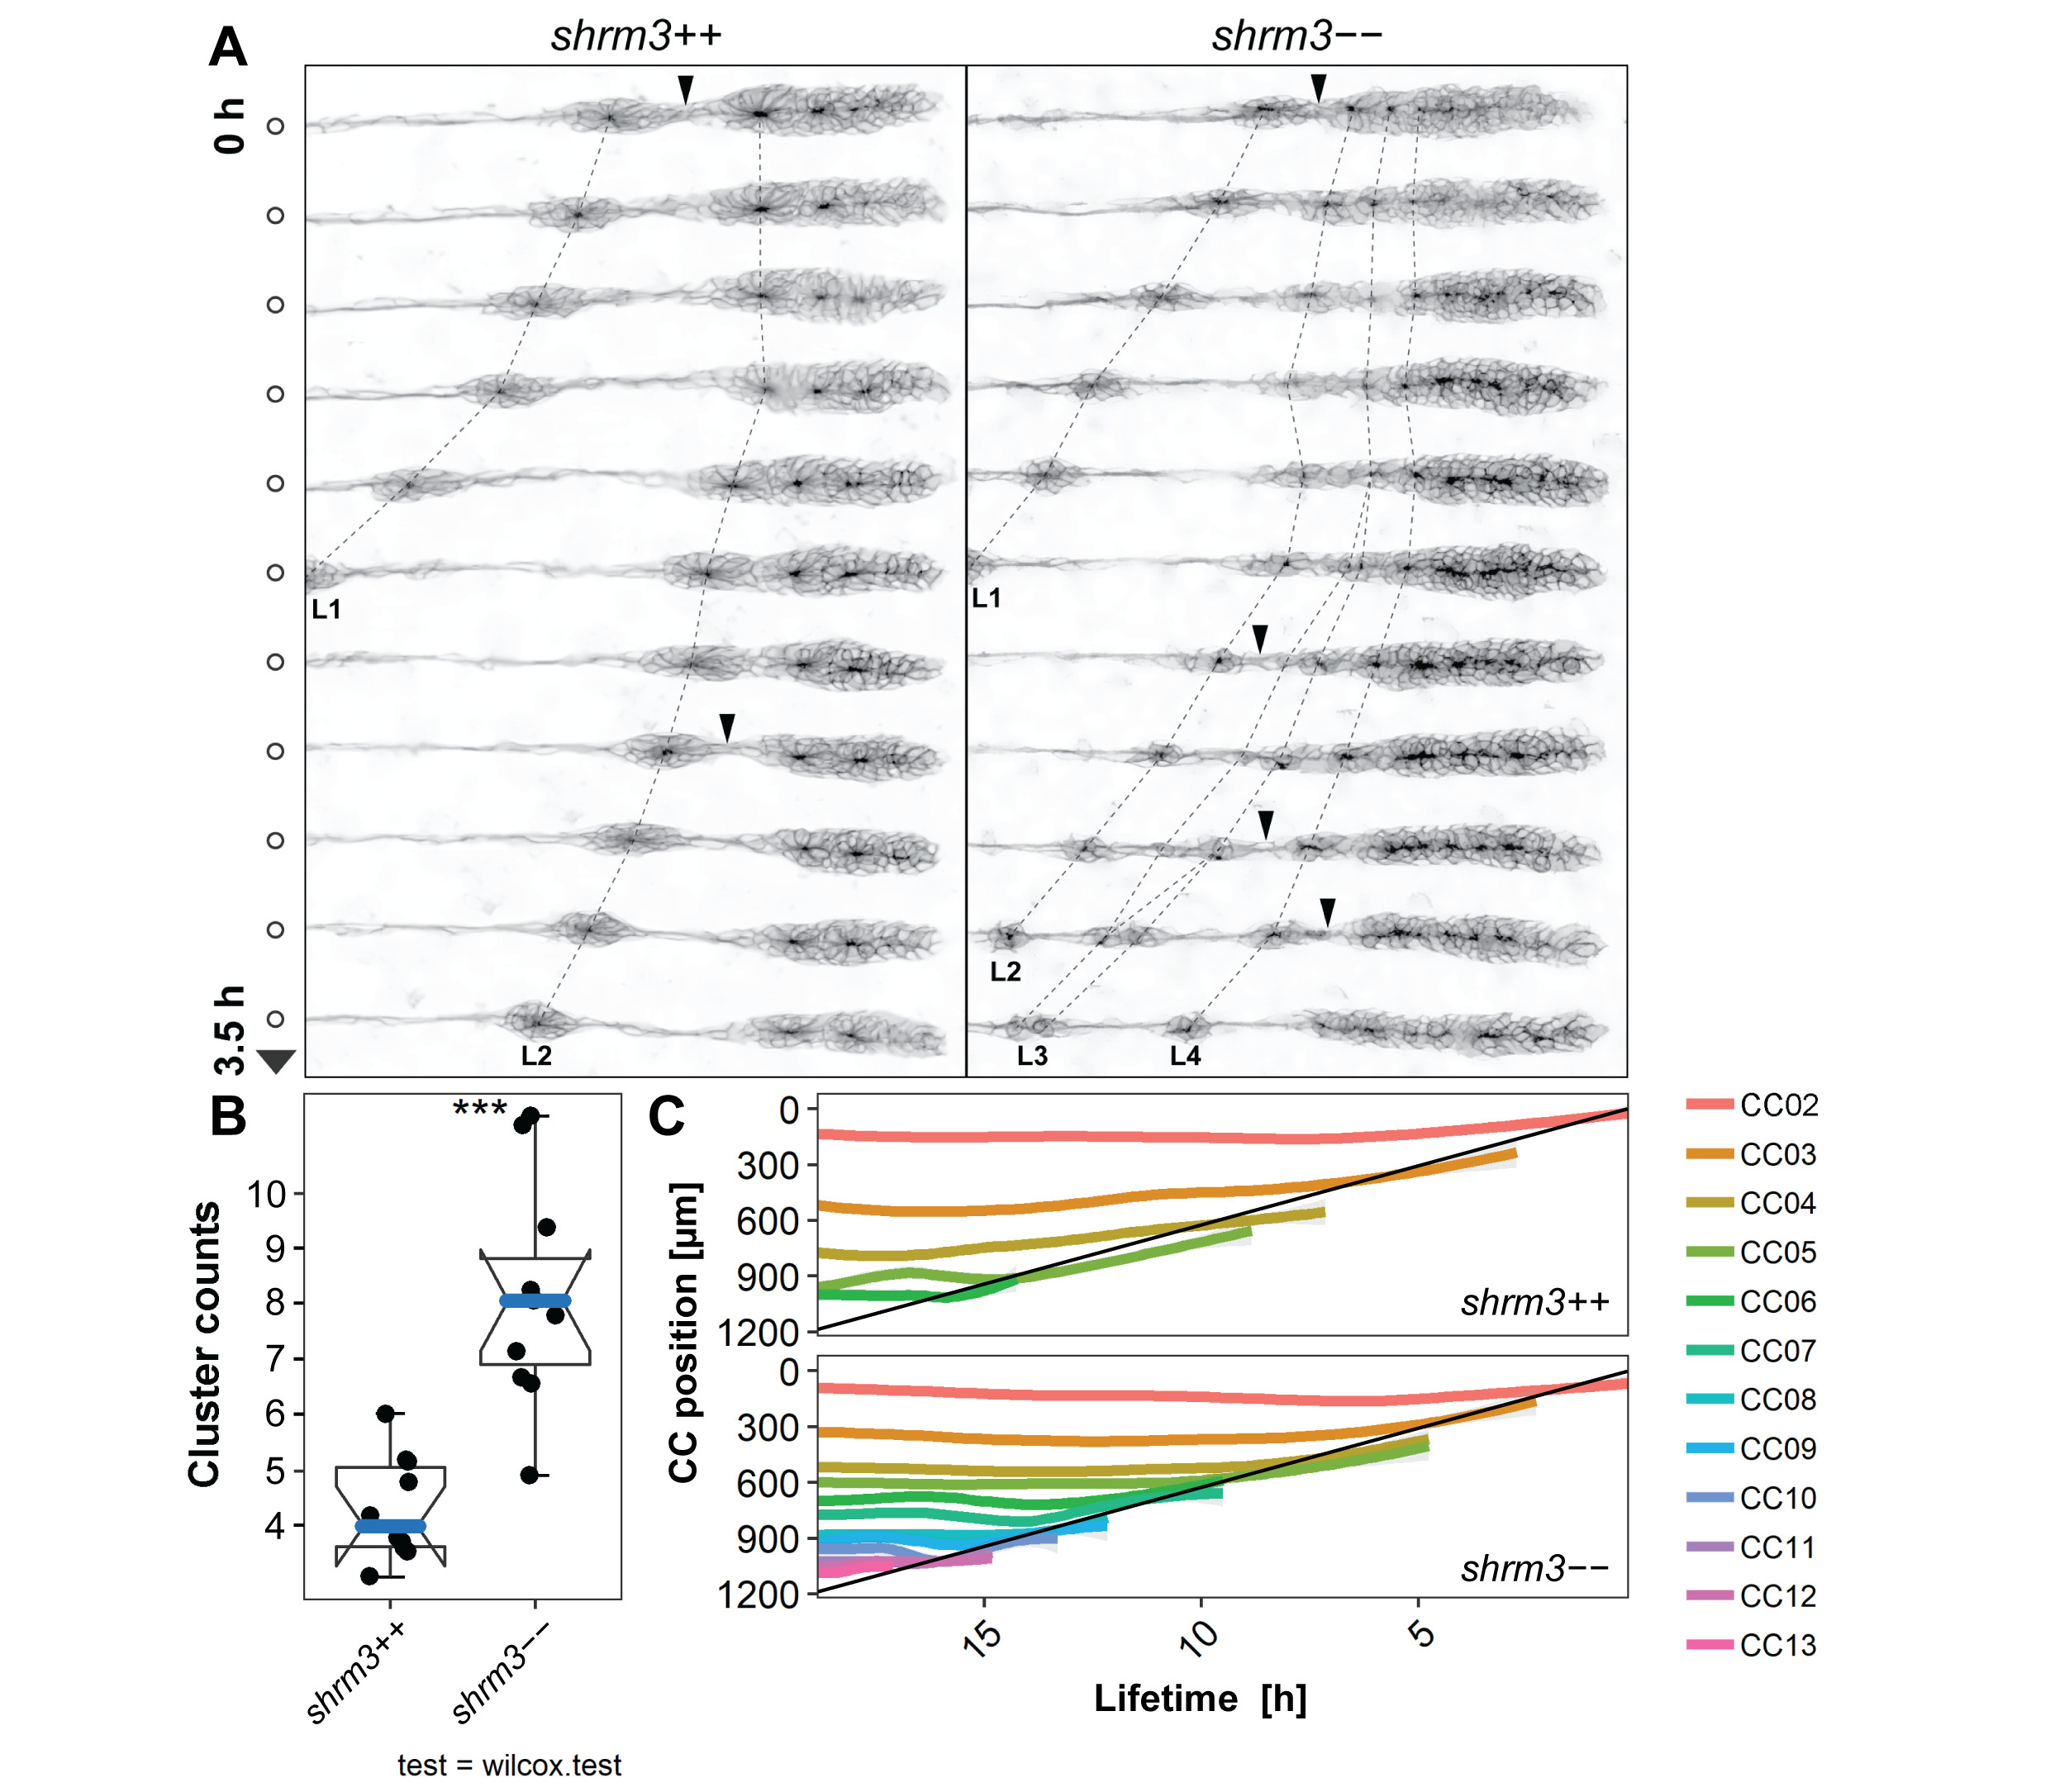
\includegraphics[width=0.95\linewidth]{figures/results/03_rosettes/tracking-01} 

}

\caption[Cluster Deposition]{Cluster Deposition. \textbf{A} \emph{shroom3}\(^{+/+}\) and \emph{shroom3}\(^{-/-}\) LL development in comparison. L1 - L4 are deposited CCs. Arrows indicate deposition events. Dotted lines are tracks of rosette to CC transition. \textbf{B} Statistics of deposited cluster counts \textbf{C} Change of CC position through time. Each line represents the locally weighted scatterplot smoothing (LOESS) of all CCn positions observed. See section \ref{res-rosreg} for a dataset description.}\label{fig:rdtdepo}
\end{figure}
On average, as it was shown in section \ref{res-ccounts}, there's a significant increase in clusters deposited (\ref{fig:rdtdepo}B). Also, neither \emph{shroom3}\(^{+/+}\) nor \emph{shroom3}\(^{-/-}\) CCs drastically change their position once they are deposited.

\hypertarget{res-rosreg}{%
\subsubsection{Registration}\label{res-rosreg}}

As the pLLP migrates it moves through space and time. To measure velocity and acceleration, one needs to detect where in space (XY coordinates) the pLLP is located at multiple timepoints. When duplicating the pLLP based on a detection ROI from the whole image, the pLLP is registered in time and space (figure \ref{fig:rdtreg}A).

As shown in figure \ref{fig:rdtreg}B-B' neither speed nor acceleration drastically differ throughout the complete course of migration. Speed drops from an initial \textasciitilde75 \(\mu\)m/h to about \textasciitilde30 \(\mu\)m/h for both \emph{shroom3}\(^{+/+}\) and \emph{shroom3}\(^{-/-}\) 17 h later (figure 3.3 A). Similarly, while there is a positive acceleration of almost \textasciitilde2 \(\mu\)m/h peaking after \textasciitilde2-3 hours, the remaining two peaks progressively get smaller (\ref{fig:rdtreg}A').
While for the area no difference can be detected (\ref{fig:rdtreg}C), interestingly the roundness is on average significantly reduced in \emph{shroom3}\(^{-/-}\) pLLPs (\ref{fig:rdtreg}D). This is also evident from the montage in figure \ref{fig:rdtdepo}A.


\begin{figure}

{\centering 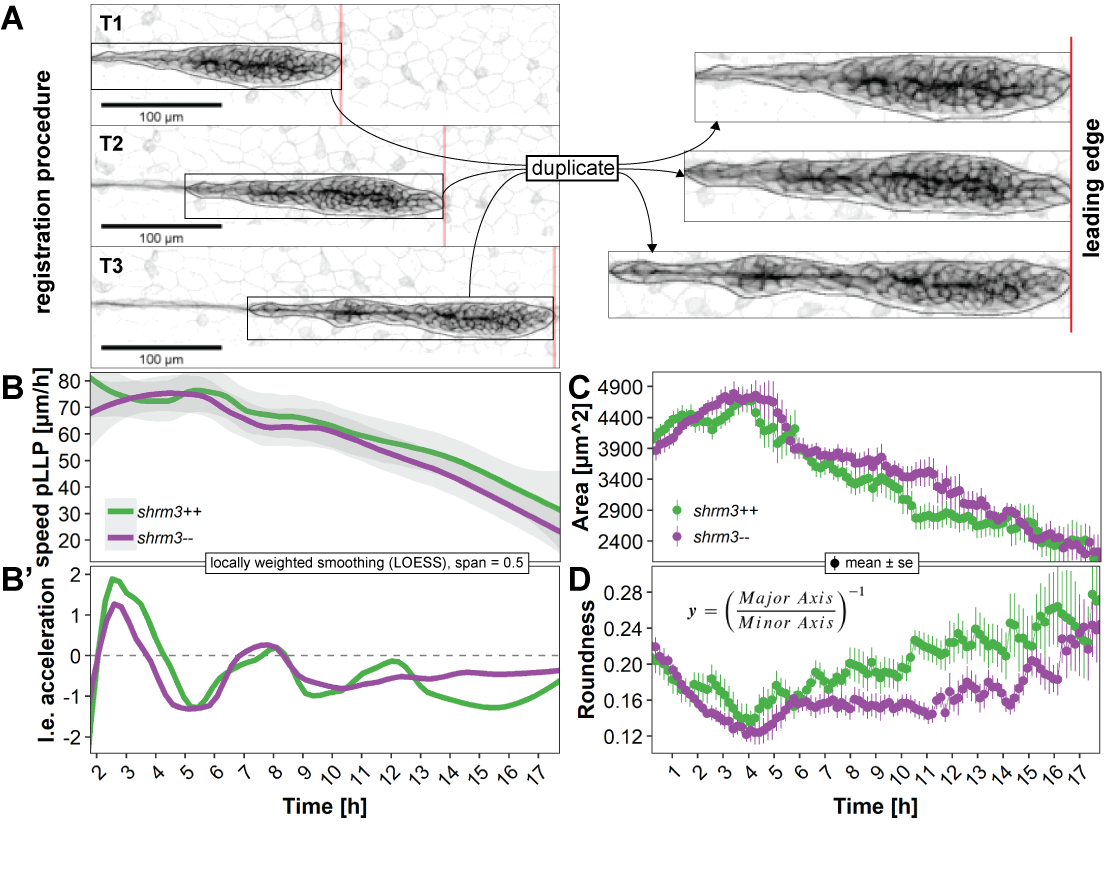
\includegraphics[width=0.95\linewidth]{figures/results/03_rosettes/registration} 

}

\caption[pLLP time-resolved morphometrics]{pLLP time-resolved morphometrics. \textbf{A} Registration procedure \textbf{B-B'} Leading edge (l.e.) speed and acceleration in \(\mu\)m/h, displayed as LOESS curves with at a span of 0.5 \textbf{C} Area in square \(\mu\)m and \textbf{D} Roundness displayed as mean ± s.e. (standard error). See section \ref{res-rosreg} for a dataset description.}\label{fig:rdtreg}
\end{figure}
\hypertarget{res-rdtdet}{%
\subsubsection{Rosette Detection}\label{res-rdtdet}}

To quantify the maturity of rosettes within the pLLP a CNN was used which allows to detect objects within images (Region Proposal based CNN). Inherent to object detection and classification by a neural network is that the network not only tells us if an object was \emph{detected} (of numbers room \(x\in[0, \infty]\subset\mathbb{N}\)), but also how secure it is - the probability - that the object detected is the right one (of numbers room \(x\in[0, 1]\subset\mathbb{R}\)) - the \emph{weighted detection}. Furthermore, the weighted detection was capped a score \(\leq\) 0.5, since below 0.5 the probability would be to insecure. In our case the network was trained to detect wildtype rosettes, while also presenting pLLPs of embryos treated with a compound that inhibits rosette formation (SU5402) to refine learning. Therefore, if the network detected 1 rosette with a probability of 0.99, it is very likely that this is a wildtype rosette. However, at different developmental stages and genetic background (e.g.~mutants with impaired rosette formation) the pLLP exhibits a different count of rosettes. Therefore it would be wrong to compare just the sum of \emph{detections} or \emph{weighted detections} per pLLP, but it is necessary to normalize for the different count of rosettes to get a global figure of pLLP rosettization - the \emph{rosettiness}.
\begin{definition}[rosettiness]
\protect\hypertarget{def:unnamed-chunk-11}{}{\label{def:unnamed-chunk-11} \iffalse (rosettiness) \fi{} }\[\frac{\sum_{} \textrm{Weighted Detections}}{\sum_{} \textrm{Detections}} = \textrm{Normalized Weight}\]
\end{definition}

\begin{figure}[H]

{\centering 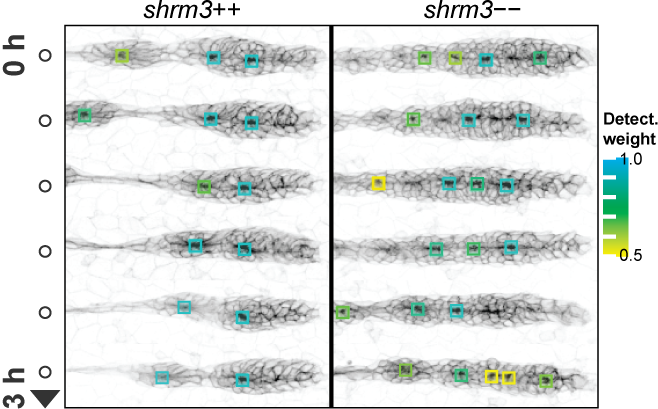
\includegraphics[width=0.95\linewidth,]{figures/results/03_rosettes/detection_model} 

}

\caption[Quantification of rosettes]{Quantification of rosettes. \textbf{A} Model of \emph{detection} and \emph{weighted detection} in \emph{shroom3}\(^{+/+}\) and \emph{shroom3}\(^{-/-}\) embryos \textbf{B} Actual detection in pLLPs of \emph{shroom3}\(^{+/+}\) and \emph{shroom3}\(^{-/-}\) embryos at six different timepoints and highlighted detection weight.}\label{fig:rdtdetmdl}
\end{figure}
The kymographs\footnote{a kymograph is a tool to record position over time} in figure \ref{fig:rdtdet}A-A' were generated from pLLPs that were previously registered with the anaLLzr2DT IJ macro (section \ref{mat-anallzr2dt}). After registration, a line was drawn along the horizontal midline (\ref{fig:rdtreg}A). Finally, recorded kymographs were turned to false color (blue = low intensity, red = high intensity) for better visual interpretation. In \emph{shroom3}\(^{+/+}\) the higher intensities are highly concentrated to two to three distinct regions within the migrating pLLP, while in the \emph{shroom3}\(^{-/-}\) pLLP the higher intensities are more fragmented and overall reduced.

The numbers reveal two very interesting things. First, the medians show that rosette count (\ref{fig:rdtreg}B') is only reduced for the first six hours, while rosettiness is reduced almost throughout the entire 20 hours. While the median rosettiness of \emph{shroom3}\(^{+/+}\) is at a constant level of about 0.9, \emph{shroom3}\(^{-/-}\) rosettiness starts out at about 0.5 but then linearly grows until it also reaches levels of about 0.9 at 16-20 hours of migration. These results, together with the finding that we could reduce the number of CCs deposited when lowering the temperature, suggests that there should be a interdependecy with speed of migration.

As for rosette detection, variance is much higher. Second, while for rosette counts comprised between 2 and 6, half or more of the pLLPs are \emph{shroom3}\(^{+/+}\), for counts below two and above six there are more \emph{shroom3}\(^{-/-}\) pLLPs (\ref{fig:rdtreg}B). Furthermore figure \ref{fig:rdtdet}C shows that at a rosettiness of \textasciitilde0.7 there are about as many \emph{shroom3}\(^{+/+}\) as there are \emph{shroom3}\(^{-/-}\) pLLPs, marking this point as a threshold were pLLPs above are more like likely to be \emph{shroom3}\(^{+/+}\) and below more likely to be \emph{shroom3}\(^{-/-}\). At \textasciitilde0.1 rosettiness there are almost only \emph{shroom3}\(^{-/-}\) pLLPs, while at \textasciitilde0.9 rosettiness there are almost only \emph{shroom3}\(^{+/+}\) pLLPs.
In addition, the data distributions is shown on the right (\ref{fig:rdtreg}B'' and C'') reveal that for the rosettiness the ditribution did not actually shift to a lower number, but rather flattened and variance is increased.


\begin{figure}

{\centering 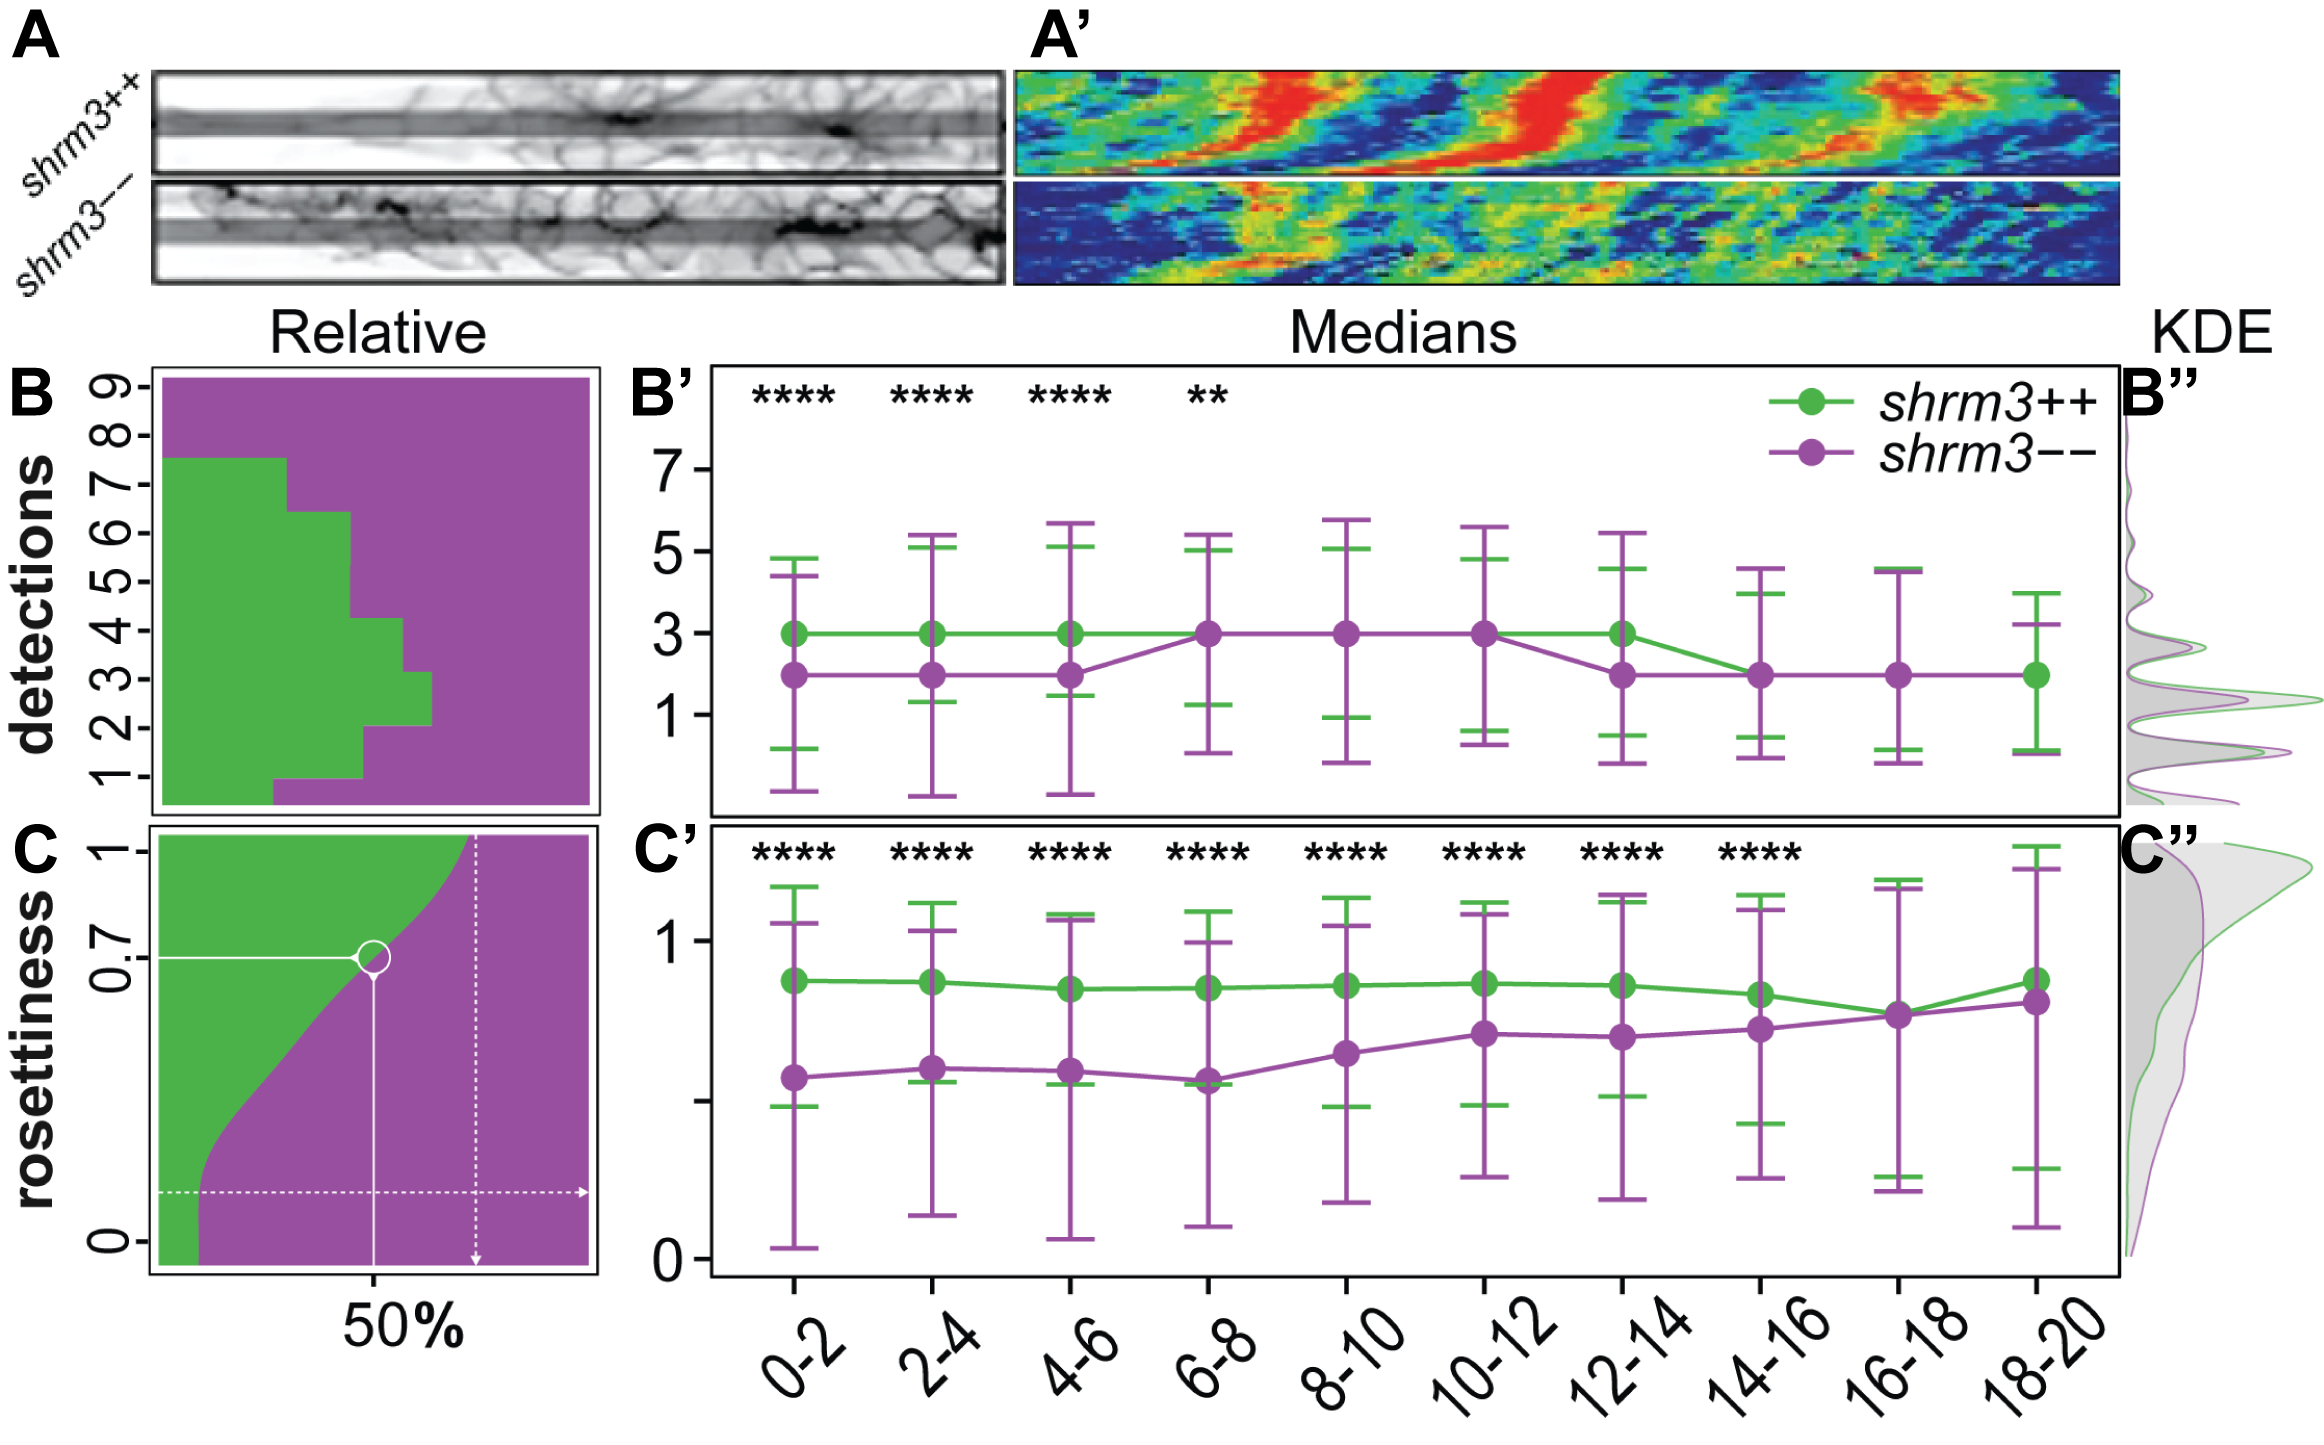
\includegraphics[width=0.95\linewidth]{figures/results/03_rosettes/detection} 

}

\caption[Rosette counts and weights]{Rosette counts and weights. \textbf{A-A'} pLLP kymographs. Length in A' = 100 \(\mu\)m. (A) shows the signal and line drawn. (A') shows the signal through time. \textbf{B-B''} Rosette detections as whole numbers (\(\mathbb{Z}\)). (B) \emph{Relative} shows the ratio of detections in \emph{shroom3}\(^{+/+}\) and \emph{shroom3}\(^{-/-}\) (x axis) at each count of detections per pLLP (y axis) throughout time. (B') \emph{Medians} shows the median \(\pm\) standard deviation of detections (y axis) as dots in time intervals of 2 h (x axis). (B'`) \emph{KDE} shows the density in the distribution of the data. \textbf{C-C''} Rosettiness as rational numbers (\(\mathbb{Q}\)). (B) \emph{Relative} shows the ratio of rosettiness in \emph{shroom3}\(^{+/+}\) and \emph{shroom3}\(^{-/-}\) (x axis) at level of rosettiness per pLLP (y axis) throughout time. At \textasciitilde70\(\%\) rosettiness the ratio of \emph{shroom3}\(^{+/+}\) over \emph{shroom3}\(^{-/-}\) is equally distributed (B') \emph{Medians} shows the median \(\pm\) standard deviation of rosettiness (y axis) as dots in time intervals of 2 h (x axis). (B'') \emph{KDE} shows the density in the distribution of the data. See section \ref{res-rosreg} for a dataset description.}\label{fig:rdtdet}
\end{figure}
\hypertarget{interdependences}{%
\subsubsection{Interdependences}\label{interdependences}}

In the previous sections I have shown that in embryos deficient for Shroom3 more NMs are deposited and that this is not caused by an overproliferation in the pLLP. In this section my goal was to collect detailed information about LL morphometrics and rosette formation to find out what is causing the additional CCs to be deposited.

To do this I combined the results of three different analyses to be able to detect inter-dependencies between variables. For my question the most interesting variable to find dependencies with is rosettiness. As mentioned in section \ref{intro-phen} when we had a first closer look at the pLLP phenotype we found that some of the clearly as \emph{shroom3}\(^{-/-}\) identified embyros still were reminiscent of the \emph{shroom3}\(^{+/+}\) phenotype. However, what surprised us the most (due to to previous results indicating an important role during rosette assembly for Shroom3), was that a fraction had significantly more CCs deposited. To test the interdependence between rosettiness and CCs deposited quantitatively we set up two hypotheses.

First, when we had a closer look at timelapse movies of the migrating pLLP at a high temporal resolution we had the impression that while in \emph{shroom3}\(^{+/+}\) embryos the pLLP stalled for a moment during CC deposition, this was not the case in \emph{shroom3}\(^{-/-}\) embryos. Therefore the hypothesis to test was that higher velocity or acceleration lead to a lower degree of rosettiness and \emph{vice versa} (figure \ref{fig:rdtcorr}A-B). While velocity is the rate at which an object moves in a certain direction, acceleration tells us the rate at which velocity changes. While most of the \emph{shroom3}\(^{+/+}\) pLLPs nicely cluster in the top right corner (high rosettiness and velocity, green dots in figure \ref{fig:rdtcorr}A), for the \emph{shroom3}\(^{-/-}\) pLLPs there is more of a spread. However, there seems to be a weak relationship between velocity and rosettiness which is also reflected by the correlation coefficient. The relationship between acceleration and rosettiness on the other hand seems to be stronger. Again, \emph{shroom3}\(^{+/+}\) pLLPs nicely cluster in the lower right corner (high rosettiness and negative acceleration, green dots in figure \ref{fig:rdtcorr}B). Since over the course of migration the pLLP gets slower (\ref{fig:rdtreg}B), the average acceleration is negative. For the \emph{shroom3}\(^{-/-}\) pLLPs there is also more of a spread, but the trend is more clearly visible which is also reflected by the correlation coefficient.

Second, since we know Shroom3 plays a role in rosette assembly and that embryos deficient for Shroom3 have on average more CCs deposited, we wanted to test if there is a direct link between the two and have statistical certainty. Therefore, the hypothesis to test for figure \ref{fig:rdtcorr}B was if lower rosettiness leads to a higher number of CCs deposited and \emph{vice versa}. Since here the end of migration cluster count is one-dimensional (one number per embryo), we had to correlate it to a \emph{per embryos} summary statistic rosettiness. Here the correlation coefficient is rather high, the interdependence seems to be true. Additionally, the clusters determined are nicely separated from each other and the \emph{shroom3}\(^{+/+}\) and \emph{shroom3}\(^{-/-}\) pLLPs seem to form two independent groups.


\begin{figure}[H]

{\centering 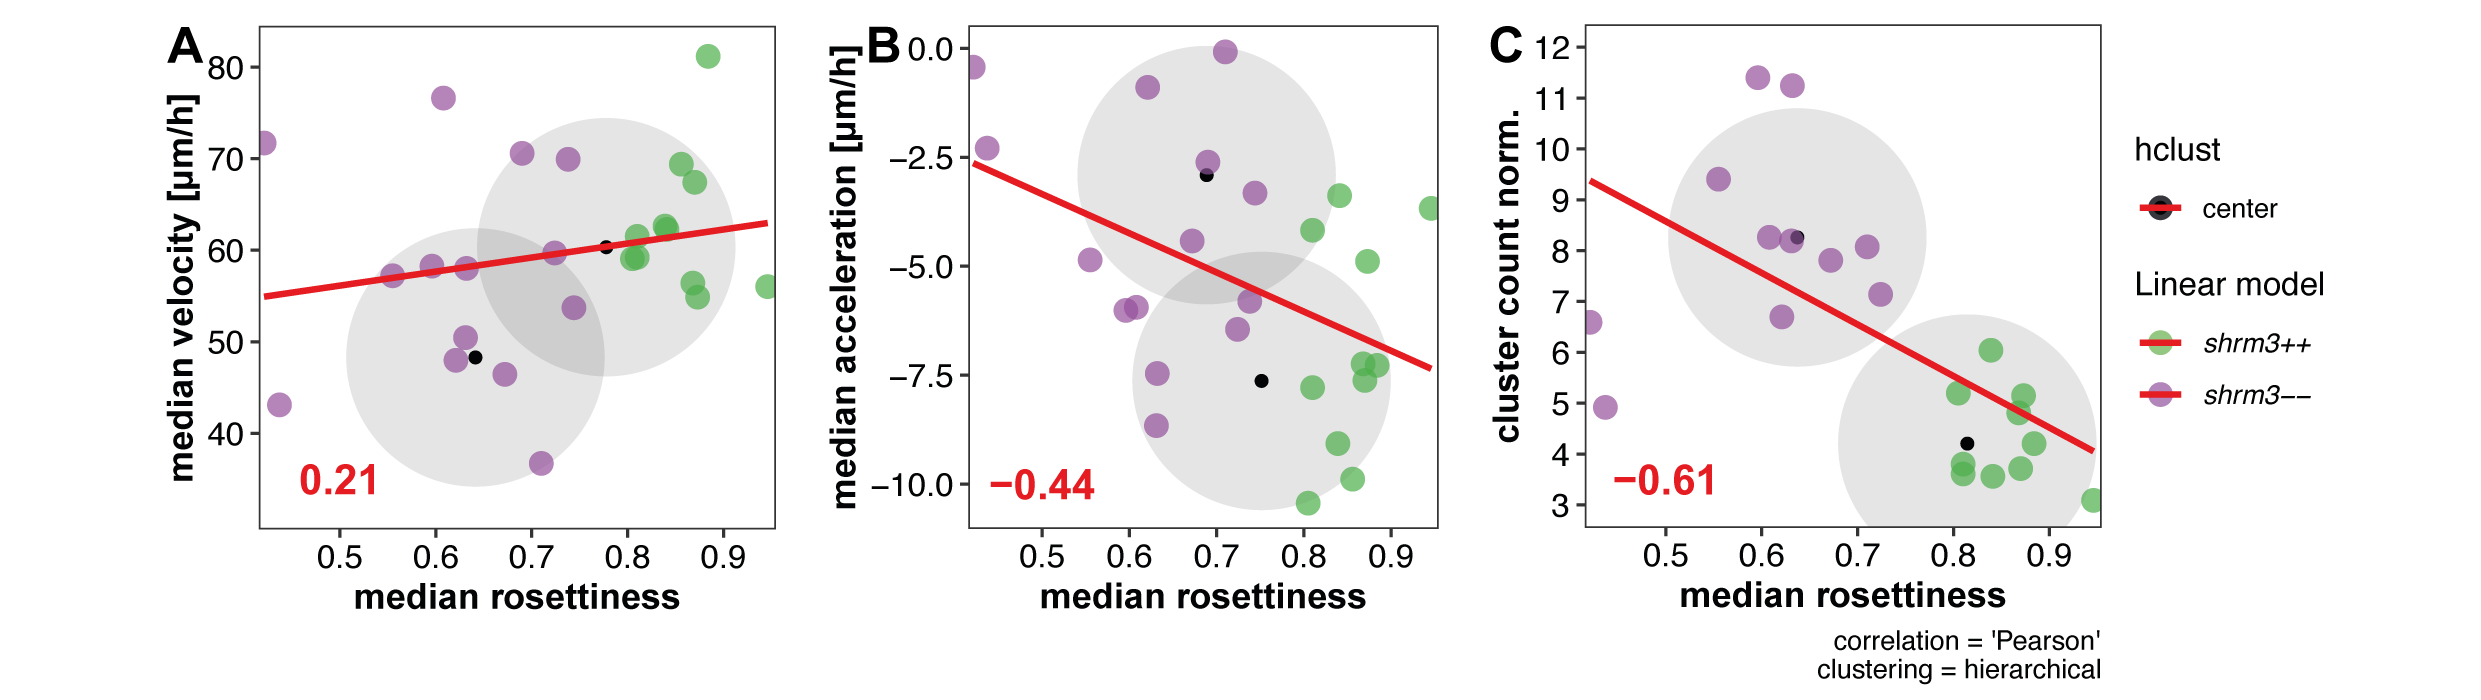
\includegraphics[width=1\linewidth]{figures/results/03_rosettes/rdt_cor_velo_acc_depo} 

}

\caption[Developmental interdependencies]{Developmental interdependencies. Single dots in the scatterplots represent the variables scatter in \(x\) and \(y\), the red line shows a linear model through the point cloud of both groups \emph{shroom3}\(^{+/+}\) and \emph{shroom3}\(^{-/-}\), red digits indicate the correlation coefficient. Black spots with grey circles indicate the centers for clusters calculated on these two sets of data. Clustering was performed hierarchical \textbf{A} Correlation between pLLP rosettiness and speed of migration \textbf{B} Correlation between pLLP rosettiness and acceleration \textbf{C} Correlation between pLLP rosettiness and number of deposited clusters normalized to the length of the lateral line.}\label{fig:rdtcorr}
\end{figure}
\hypertarget{res-rockresc}{%
\subsubsection{Mechanics}\label{res-rockresc}}

It is very well known that Rho kinases are necessary for mechanic force transmission in various developmental processes (\emph{26}, \emph{44}, \emph{49}, \emph{78}, \emph{79}). Since Rock is also thought to be a key player of the Shroom force mediation pathway in the pLLP, the idea for a mechanic rescue was to titrate different concentrations of a Rock inhibitor (Rockout, section \ref{mat-chem}) and a non-muscle myosin II (NMII) activator (Calyculin, section \ref{mat-chem}) to see if this way can confirm the correlation between rosettiness and CC number in an independent manner.

\hypertarget{rock-inhibition}{%
\paragraph{Rock inhibition}\label{rock-inhibition}}

Rock2a, upon interaction with Shroom3, phosphorylates NMII which is necessary for contraction of the actin network and apical constriction (section @ref\{intro-shroom\}). Here we wanted to mimic the \emph{shroom3}\(^{-/-}\) phenotype in \emph{shroom3}\(^{+/+}\) embryos.

Embryos were incubated at distinct (figure \ref{fig:rescrock} legend) concentrations from 24 hpf till end of migration (about 60 hpf). At this stage embryos incubated at higher concentrations displayed a significant reduction in overall body length (\ref{fig:rescrock}A'). Therefore, to see if there is a specific effect on length, LL length was normalized to body length.


\begin{figure}[H]

{\centering \includegraphics[width=0.95\linewidth]{figures/results/06_rescues/rockout/rescue_rockout} 

}

\caption[Rescue: Titration of Rock inhibitor]{Titration of Rock inhibitor. \textbf{A} LL lengths are reduced with increased concentrations of Rock inhibitor and \textbf{B} groupwise comparison of the length normalized cluster count per concentration of FGF inhibitor.}\label{fig:rescrock}
\end{figure}
Rockout treatment at 10 \(\mu\)M does not lead to a significant reduction in LL length but does significantly increase the number of CCs deposited, confirming the current hypothesis that Shroom3 acts though Rock.\newline
\begin{table}

\caption{\label{tab:rescrocktab}Rockout rescue dataset summary}
\centering
\fontsize{10}{12}\selectfont
\begin{tabu} to \linewidth {>{\raggedleft}X>{\centering}X>{\raggedright}X}
\toprule
genotype & conc. ($\mu$M) & LLs\\
\midrule
 & 0 & 17\\

 & 10 & 13\\

 & 50 & 17\\

\multirow[t]{-4}{*}{\raggedleft\arraybackslash \textit{shroom3}++} & 100 & 20\\
\bottomrule
\multicolumn{3}{l}{\textit{conc.}}\\
\multicolumn{3}{l}{concentrations in 0.1\% DMSO solution}\\
\end{tabu}
\end{table}
\hypertarget{nmii-activation}{%
\paragraph{NMII activation}\label{nmii-activation}}

Downstream of Shroom3 NMII, as a motor protein, is necessary for contraction of the actin network and apical constriction (section @ref\{intro-shroom\}). The idea for this experiment was to rescue the \emph{shroom3}\(^{-/-}\) phenotype by over-activation of NMII. Unfortunately, even when incubation at 100 nM (the maximum solubility), no significant differences can be detected.\newline


\begin{figure}[H]

{\centering \includegraphics[width=0.85\linewidth]{figures/results/06_rescues/caliculyn/rescue_cali} 

}

\caption[Calyculin treatment]{NMII activation. \textbf{A} LL lengths and \textbf{B} groupwise comparison of the length normalized cluster count.}\label{fig:resccal}
\end{figure}
\begin{table}

\caption{\label{tab:resccaltab}NMII activation dataset summary}
\centering
\begin{tabu} to \linewidth {>{\centering}X>{\centering}X>{}c|>{\centering}X>{\centering}X>{\centering}X}
\toprule
genotype & conc. (nM) & LLs & genotype & conc. (nM) & LLs\\
\midrule
 & 0 & 8 &  & 0 & 8\\

\multirow[t]{-2}{*}{\centering\arraybackslash \textit{shroom3}++} & 100 & 12 & \multirow[t]{-2}{*}{\centering\arraybackslash \textit{shroom3}$--$} & 100 & 12\\
\bottomrule
\multicolumn{6}{l}{\textit{conc.}}\\
\multicolumn{6}{l}{concentrations in 0.1\% DMSO solution}\\
\end{tabu}
\end{table}
\hypertarget{summary-4}{%
\subsubsection{Summary}\label{summary-4}}

I could (\textbf{1}) demonstrate, from fixed embryos (figure \ref{fig:llcounts}B) as well as here on live imaging data (figure \ref{fig:rdtdepo}B), that in \emph{shroom3} heterozygous mutants significantly more CCs are deposited, gaining more insight in the deposition process which shows smaller and more fragmented CCs and a more chaotic deposition process overall (figure \ref{fig:rdtdepo}A) (\textbf{2}) show a possible interdependence with velocity and acceleration (figure \ref{fig:rdtcorr}A-B). Also the area of the pLLP is not affected, but roundness, confirming our impression that the pLLP in \emph{shroom3}\(^{-/-}\) embryos is more elongated (figure \ref{fig:rdtreg}C-D) (\textbf{3}) show that while the integer number of rosettes in the pLLP is only significantly increased during the first 6-8 hours of migration, the overall \emph{rosettiness} (rosette integrity per pLLP) is significantly reduced over the whole path of migration (figure \ref{fig:rdtdet}C').

Rosettiness is strongly correlated to the final number of CCs deposited (\ref{fig:rdtcorr}C), concluding that rosettiness is the key parameter for the future outcome of CC pattern. Interestingly however this conclusion contradicts the previous, and intuitive, assumption that embryos deficient for Shroom3 should not deposit CCs at all. However, in the light of this data Shroom3 is important to strengthen rosette integrity in order to have CCs of the right size deposited.

Still, the question is: What determines rosette weight? Velocity and rosettiness are correlated weaker than acceleration and rosettiness are which indicates that the rate at which velocity changes has more of an impact than velocity itself. This finding is also confirmed by an experiment where the CC count of \emph{shroom3}\(^{-/-}\) can be rescued when incubated at lower temperature (section \ref{res-tempresc}).

\hypertarget{apical-constriction-3}{%
\subsection{Apical Constriction}\label{apical-constriction-3}}

In the previous analysis I have shown a direct relationship between rosette integrity and CCs deposited, where lower rosette integrity leads to a fragmented rosettes and therefore to an increase in CC deposition frequency. To preserve rosette integrity and for proper CC maturation cells need to apically constrict. To gain further insight into Shroom3 contribution to apical constriction, it is appropriate to have a closer look at rosette conformation on a cellular scale. To do so, first a set of high spatial resolution, volumetric image data was generated (XY = 0.164 \(\mu\)m / pixel; Z = 0.4 \(\mu\)m) that allowed for\ldots{}
\begin{enumerate}
\def\labelenumi{\arabic{enumi}.}
\tightlist
\item
  a more rigorous inspection of morphological differences, and
\item
  automated and unbiased single cell 3D reconstruction (section \ref{ACI-singlecell}) using a newly developed IJ macro (section \ref{mat-anallzr3d}). Secondly, to investigate the contribution of various single cell morphometrics to rosette formation an app was developed\footnote{LLMapR - dskleinhans.shinyapps.io/LLmapR} that allows for a convenient handling of large amounts of retrieved data.
\end{enumerate}

\begin{figure}[H]

{\centering \includegraphics[width=0.95\linewidth]{figures/results/04_constriction/reconstriction_data} 

}

\caption[High resolution, volumetric image data]{High resolution, volumetric image data. Upper row shows the fluorescence signal at the membranes. Lower row shows the 3D reconstructed cells. Columns show the same pLLP from different angles.}\label{fig:acdata}
\end{figure}
Inhibition of FGFR1 \emph{via} drug treatment (SU5402, section \ref{mat-chem}) results in a concentration dependent loss of morphogenesis and rosette assembly in the pLLP (\emph{38}, \emph{40}, \emph{61}). As a proof of principle and to validate previous studies, data of drug treated embryos (20 \(\mu\)M) and appropriate DMSO (0.1\(\%\) DMSO / E3\footnote{`Embryo Medium 3', section \ref{mat-buff}}) controls were included.

\hypertarget{dataset-1}{%
\subsubsection{Dataset}\label{dataset-1}}

The dataset generated consists of three pLLP stages (\ref{fig:acstages}), four groups (DMSO, SU5402, \emph{shrm3}++ and \emph{shroom3}\(^{-/-}\)), 267 pLLPs and 33.163 single cells.\newline


\begin{figure}[H]

{\centering \includegraphics[width=0.6\linewidth]{figures/results/04_constriction/Yolk_ext} 

}

\caption[Recorded developmental stages for 3D reconstruction]{Scheme showing a part of the posterior part of a zebrafish embryo and recorded developmental stages for 3D reconstruction}\label{fig:acstages}
\end{figure}
\begin{table}

\caption{\label{tab:acdatatab}Apical Constriction dataset summary}
\centering
\begin{tabu} to \linewidth {>{\raggedright}X>{\raggedright}X>{\centering}X>{\centering}X>{\centering}X}
\toprule
\multicolumn{2}{c}{\textbf{id labels}} & \multicolumn{3}{c}{\textbf{metrics}} \\
\cmidrule(l{3pt}r{3pt}){1-2} \cmidrule(l{3pt}r{3pt}){3-5}
stage & group & pLLPs & cells & ratio\\
\midrule
 & DMSO & 20 & 2511 & 125.5\\

 & SU5402 & 19 & 2215 & 116.6\\

 & \textit{shroom3}++ & 24 & 3259 & 135.8\\

\multirow[t]{-4}{*}{\raggedright\arraybackslash 32 hpf} & \textit{shroom3}$--$ & 34 & 4281 & 125.9\\

 & DMSO & 17 & 1881 & 110.6\\

 & SU5402 & 13 & 1286 & 98.9\\

 & \textit{shroom3}++ & 24 & 3144 & 131.0\\

\multirow[t]{-4}{*}{\raggedright\arraybackslash 36 hpf} & \textit{shroom3}$--$ & 31 & 3924 & 126.6\\

 & DMSO & 18 & 2237 & 124.3\\

 & SU5402 & 13 & 1788 & 137.5\\

 & \textit{shroom3}++ & 22 & 2660 & 120.9\\

\multirow[t]{-4}{*}{\raggedright\arraybackslash 40 hpf} & \textit{shroom3}$--$ & 32 & 3977 & 124.3\\
\bottomrule
\multicolumn{5}{l}{\textit{ratio}}\\
\multicolumn{5}{l}{cells / pLLPs}\\
\end{tabu}
\end{table}
\hypertarget{shape-and-arrangement}{%
\subsubsection{Shape and Arrangement}\label{shape-and-arrangement}}

Figure \ref{fig:acshape}B' illustrates the three developmental stages used for this analysis. For \emph{shroom3}\(^{+/+}\) pLLPs two (\ref{fig:acshape}A, 32 hpf) to four (\ref{fig:acshape}A, 40 hpf) areas of constricting regions can be observed (XZ pane), in \emph{shroom3}\(^{-/-}\) its three (\ref{fig:acshape}A, 36 hpf) to seven (\ref{fig:acshape}A, 40 hpf), confirming the results of rosette detection (\ref{res-rdtdet}). While at 32 and 36 hpf the spread of those regions (indicated by bars in \ref{fig:acshape}, XZ panes) is wider in \emph{shroom3}\(^{-/-}\), at 40 hpf they are smaller but also increased in number. When looking at the central rosette along the width ((indicated by arrows in \ref{fig:acshape}), YZ panes), it seems like there is no considerable difference between \emph{shroom3}\(^{+/+}\) and \emph{shroom3}\(^{-/-}\) rosettes. In SU5402 treated embryos, neither in XZ nor in YZ constriction can be observed and the cells seem to be mostly columnar in shape. In addition, while constriction seems isotropic in the \emph{shroom3}\(^{+/+}\) rosette center, constriction in the \emph{shroom3}\(^{-/-}\) rosette center cells appears anisotropic.


\begin{figure}[H]

{\centering \includegraphics[width=0.95\linewidth]{figures/results/04_constriction/Figure_5-1} 

}

\caption[Apical Constriction in 3D]{Apical Constriction in 3D. \textbf{Stages are in columns}, the \textbf{groups are in rows}. Each panel shows a MaxIP (top left), and orthogonal views along the length (XZ, bottom left) and the width (YZ, right). Arrow annotations in YZ panels indicate points of constriction. Bar annotations in XZ indicate the spread of region of constriction.}\label{fig:acshape}
\end{figure}
\hypertarget{height}{%
\subsubsection{Height}\label{height}}

Earlier attempts for indexing AC include measuring the `apical index' (A.I.) of bottle cells during \emph{X.laevis} gastrulation (\emph{80}) or for cells of the pLLP (\emph{61}). For both, the metric describes the ratio of lateral height over apical width which, depending on the situation, is a very coarse and inaccurate description. In the pLLP cells of different forms, volumes and heights can be found. When measuring apical width at a fix distance from the apical site cells with different height but otherwise equal degree of AC turn out to have a very different A.I. (figure \ref{fig:ACICells}A and A'). If however apical width is measured at a distance relative to the cells height, cells with an equal degree of AC turn out to have the same A.I. (figure \ref{fig:ACICells}A and A''). In addition, it remains questionable exactly how to define \emph{apical width} in a two-dimensional cellular cross-section. By introducing apical width measurement along both, the major and the minor axis (section \ref{ACI-pol}), the improved model for AC and method for automated and unbiased cellular segmentation therefore represents a major advancement.

For another demonstration of the method figure \ref{fig:dismap} shows a heatmap of cell height, how its distributed in the pLLP and under different conditions. At stages 32 and 36 hpf, height in \emph{shroom3}\(^{-/-}\) cells is not as strongly reduced as in SU5402 treated ones and cells in the central region of the pLLP are higher than in the leading, trailing and lateral regions. Therefore this representation also gives an idea which cells are most affected.


\begin{figure}[H]

{\centering \includegraphics[width=0.95\linewidth]{figures/summary/methodology_mapr} 

}

\caption[pLLP Maps]{pLLP terrain maps. To get a more detailed impression about how variables are distributed within the cells of the pLLP, single cell measurements of pLLPs that are normalized in orientation can be superimposed in a two-dimensional map of organ length and width. Next, cell coordinates are grouped into bins of hexagons and the summary statistic is represented in color. (bottom right) link to the LLMapR web-app.}\label{fig:dismap}
\end{figure}
\hypertarget{res-ai}{%
\subsubsection{A.I.}\label{res-ai}}

To get a hold on AC anisotropy we measured the length of the minor and major axis of an ellipsoid fitted to the imaging Z-plane at a certain distance from the cell apex (as described in section \ref{ACI-pol} and illustrated in figure \ref{fig:acaci}A). The angle formed by the major axis of the ellipsoid and the horizontal midline indicate the orientation of AC (figure \ref{fig:acaci}A'). If more cells are constricted along the DV axis, we expect angles closer to 0\(^\circ\). If more cells are constricted along the AP axis, we expect angles closer to 90\(^\circ\). For angle measurements, all angles are normalized to a 90\(^\circ\) range, where 0\(^\circ\) is along the horizontal midline.

When comparing the ratio of cells in intervals of 15\(^\circ\) along a range of 90\(^\circ\) it can be shown that there are more \emph{shroom3}\(^{-/-}\) than \emph{shroom3}\(^{+/+}\) cells within the 0-15\(^\circ\) interval through all three stages (\ref{fig:acstages}). Even more, it shows that there are more \emph{shroom3}\(^{+/+}\) than \emph{shroom3}\(^{-/-}\) cells within the remaining intervals -- confirming the model of anisotropic constriction along the DV axis.

While \emph{reduction} in A.I.\textsubscript{Major} is stronger than the A.I.\textsubscript{Minor} in \emph{shroom3}\(^{-/-}\) cells (\ref{fig:acaci}C-C'), both are significantly reduced throughout time -- again confirming the increase in constriction an-isotropy. For all three timepoints the A.I. for SU5402 treated embryos is not only the smallest, but also stays at the same level (\textasciitilde2 in the A.I.\textsubscript{Major}, \textasciitilde3.4 in the A.I.\textsubscript{Minor}), therefore it can be seen as a lower threshold. Interestingly, the A.I.s for DMSO, \emph{shroom3}\(^{+/+}\) and \emph{shroom3}\(^{-/-}\) are progressively converging this threshold from earlier to later stages.


\begin{figure}

{\centering \includegraphics[width=0.95\linewidth]{figures/results/04_constriction/Figure_5-2} 

}

\caption[3D metrics and pLLP maps]{Apical constriction metrics. \textbf{A-A'} Measurements. (A) Oval (black outline) represents the fit ellipse. Red arrows represent major and minor axes which are representative for A-P and D-V respectively (A') Angle measurements and intervals \textbf{B} Cellular orientation as bar chart. The y axis represents the (normalized) fraction of cells per cells in the whole organ. p-value levels (wilcox-test) are indicated as stars. \textbf{C-C'} Apical Constriction measurements. Colored bars represent the median. Errorbars indicate 95\(\%\) CI.}\label{fig:acaci}
\end{figure}
\hypertarget{sum-ai}{%
\subsubsection{Summary}\label{sum-ai}}

In the previous chapter I could show that the main reason for the additional CCs deposited in Embryos deficient for Shroom3 is reduced rosettiness. Here I wanted to get a more detailed view on how rosette configuration and cell morphology compares between wildtype and mutant.

The method developed to quantify AC allows measurement along two orthogonal axes, the major (the longer axis) and a minor (the shorter axis), of an ellipse fit to a cellular cross-section at a distinct distance from the apical site. In addition, the cells orientation in degrees from the horizontal midline is obtained (\ref{fig:acaci}A-A').

In summary, AC is significantly reduced in \emph{shroom3}\(^{-/-}\) embryos. The results show an increased axial an-isotropy, meaning that AC is more reduced along the major than along the minor axis. In conclusion this means that due to less tight rosette packing and apical constriction the migrational pulling forces are probably accounting for the an-isotropy. In terms of cell shape this means that rosette cells go from a pyramidal geometry, more to a prism geometry (\ref{fig:sumcells}). This is also confirmed by angular measurement which show that in \emph{shroom3}\(^{-/-}\) pLLPs there are more cells in the range of 0-15\(^\circ\) while in \emph{shroom3}\(^{+/+}\) pLLPs more cells are in the range of 30-45\(^\circ\).


\begin{figure}

{\centering \includegraphics[width=0.9\linewidth]{figures/summary/cell-model} 

}

\caption[Rosette and Cell Shape Model]{Rosette and Cell Shape Model. Shapes reconstructed from real cells.}\label{fig:sumcells}
\end{figure}
Zona occludens-1 (ZO-1) is a peripheral membrane, tight-junction associated protein. Within the apical region of pLLP rosettes FGF filled luminal structures are developing that are hubs for locally confined morphogen signaling. All cells of a rosette make up and are connected to a single lumen. When visualizing the lumen \emph{via} an antibody for ZO-1, the lumen appears like a buckyball where each side is the connection to a single cell (\emph{40}). While in \emph{shroom3}\(^{+/+}\) rosettes those structures appear circular in the trailing rosette, in \emph{shroom3}\(^{-/-}\) rosettes they appear more oval (supplement, (\ref{fig:suppzo1}), which supports the theory of an-isotropy. Furthermore, in more leading regions the signal is more fragmented, which supports the theory of micro-rosette structures.

\hypertarget{res-hc}{%
\subsection{Haircell Specification}\label{res-hc}}

In the analyses presented so far I have shown that embryos deficient for Shroom3 deposit more CCs, that this is caused by a fragmentation of rosettes (not by overproliferation) and that AC, which is important for CC maturation, is only partially diminished (more in A-P than in D-V axis). Since we also observe a shift in cell geometry from a pyramidal to a more prism geometry, we wanted to know if this had downstream consequences on hair-cell (HC) specification.

As described in section \ref{intro-morph}, the shape of a cell has direct impact on its ability to perceive and react to external cues. Here we were interested to test if the reduction in AC (change in cell shape, section \ref{ACI-pol}) in the pLLP had an impact on HC specification and therefore if the LLs function as a sensory system would still be intact. Atoh1a (section \ref{intro-atoh}, a TF that gives cells the potential to become sensory HCs), in the pLLP is locally expressed between leader and follower cells and is finally restricted to a single center cell \emph{via} lateral inhibition (section \ref{intro-notch}). Since till today it was not shown why the center cell becomes the HC - here our hypothesis was that rosette assembly (radial organization) respectively AC could play a role.

First, to check if \emph{atoh1a} was still expressed in \emph{shroom3}\(^{-/-}\) cells and if there were further implications in feedback loops with Notch signaling, an \emph{In Situ Hybridization} (ISH, section \ref{ISH-met}) experiment was conducted (probes in section \ref{mat-probes}). For 36 and 40 hpf the count of \emph{atoh1a} and \emph{deltaD} expressing cells (\ref{fig:hcish}) seemed to be increased. Furthermore, especially at 40 hpf, the signal seems to be a lot more fragmented and fuzzier.


\begin{figure}

{\centering \includegraphics[width=0.85\linewidth]{figures/results/05_atoh/hc_ish} 

}

\caption[Expression of deltaD and atoh1a in the pLLP]{Expression of deltaD and atoh1a in the pLLP. Recorded in greyscale at brightfield at 20X Magnification. Images show background subtracted and de-noised EDFs of original Z-stack data.}\label{fig:hcish}
\end{figure}
Traditional ISH allows for detection of RNA transcripts on a whole embryo scale \emph{via} a hybridizing anti-sense probe. However, since embryos are fixed, it only allows to analyze single time points. Furthermore, since images are taken in brightfield, quantification of signal intensity is difficult and since what is visualized is a precipitate rather than a signal there is not a clear linear relationship to quantify the amount of expression.

To get access to developmental dynamics we made use of an additional, besides \emph{cldnb:lyn-gfp}, transgenic construct where tdTomato (\emph{81}) is expressed under direct control of the \emph{atoh1a} promotor. By simultaneous observation of both fluorophores in a time-lapse setup (\ref{fig:hctl}B), the strategy was to follow up the dynamics of tdTomato to quantify the expression of \emph{atoh1a} in cell count and intensity of expression.

\hypertarget{dataset-2}{%
\subsubsection{Dataset}\label{dataset-2}}

For each group, \emph{shroom3}\(^{+/+}\) and \emph{shroom3}\(^{-/-}\), and timepoint the dataset was split into pLLP and CC (table \ref{tab:hcdatatab}). Each time-lapse has a duration of 18-20 hours, consists of about 54 timepoints and two channels (488 \& 561 nm).\newline
\begin{table}

\caption{\label{tab:hcdatatab}Hair-cell specification dataset summary}
\centering
\begin{tabu} to \linewidth {>{\raggedright}X>{\raggedright}X>{\centering}X>{\centering}X>{\centering}X}
\toprule
\multicolumn{2}{c}{\textbf{id labels}} & \multicolumn{3}{c}{\textbf{metrics}} \\
\cmidrule(l{3pt}r{3pt}){1-2} \cmidrule(l{3pt}r{3pt}){3-5}
genotype & sub-structure & embryos & timepoints & per 3h\\
\midrule
 & pLLP & 28 & 1566 & 261\\

\multirow[t]{-2}{*}{\raggedright\arraybackslash \textit{shroom3}++} & CC & 28 & 2499 & -\\

 & pLLP & 21 & 1134 & 189\\

\multirow[t]{-2}{*}{\raggedright\arraybackslash \textit{shroom3}$--$} & CC & 21 & 3566 & -\\
\bottomrule
\end{tabu}
\end{table}
\hypertarget{atoh1a-in-the-ll}{%
\subsubsection{Atoh1a in the LL}\label{atoh1a-in-the-ll}}

While in both \emph{shroom3}\(^{+/+}\) and \emph{shroom3}\(^{-/-}\) tdTomato signal intensities are rising as soon as CCs are deposited (figure \ref{fig:hctl}A), in \emph{shroom3}\(^{-/-}\) pLLPs intensities are on the rise already in the first four hours of migration. Comparing signal intensities in deposited CCs for both, \emph{shroom3}\(^{+/+}\) and \emph{shroom3}\(^{-/-}\) show a similar pattern of increasing tdTomato signal intensity over the course of development but decreasing tdTomato signal intensity at the timepoint of deposition with progressive CC depositions (figure \ref{fig:hctl}B). Similarly, when looking at ungrouped CC signal intensity (not \emph{per} CC, but as one group), no difference can be detected (figure \ref{fig:hctl}C).

While there is no difference in relative numbers of \emph{atoh1a} expressing cells within the migrating pLLP throughout time (figure \ref{fig:hctl}D), when comparing mean \emph{atoh1a} expressing cell counts at specific intervals (about the deposition frequency) the \emph{shroom3}\(^{-/-}\) line is always on or above the \emph{shroom3}\(^{+/+}\) line (figure \ref{fig:hctl}D'), indicating significantly more \emph{atoh1a} expressing cells in \emph{shroom3}\(^{-/-}\) pLLPs.

The extrusions to the left in the Kymographs in figure \ref{fig:hctl}D are representative to the elongating pLLP during the process of CC deposition. Magenta curves represent expression of \emph{atoh1a}. For the \emph{shroom3}\(^{-/-}\) pLLP, premature expression of \emph{atoh1a} can be detected. The diagonal lines in the kymographs in figure \ref{fig:hctl}D' represent the moving pLLP along the LL. Vertical curves represent deposited CCs. As for the registered pLLP, Magenta curves represent expression of \emph{atoh1a}.


\begin{figure}

{\centering \includegraphics[width=0.95\linewidth]{figures/results/05_atoh/ato-tom} 

}

\caption[Hair-cell specification in the LL]{Hair-cell specification in the LL.\textbf{A} Sample of imagaes analyzed. \emph{upper panel} shows the \emph{cldnb:lyn-gfp} transgene with segmentation masks highlighted in red. Each structure is labeled with the corresponding label in the tabular data. \emph{lower panel} shows the \emph{atoh1a:Tom} transgene with segmentation mask transferred from upper panel. \textbf{B and C} Maximum tdTomato intensities in the pLLP and CCs. All CC lifetimes were normalized to the timepoint of deposition (timepoint zero, highlighted by striped vertical line). pLLP intensities are shown to the right (black curve), CC intensities are shown on a negative scale to the left (colored curves). \textbf{D} Relative numbers of \emph{atoh1a} expressing cells to number of timepoints and \textbf{D'} mean counts of \emph{atoh1a} expressing cells. \textbf{D-D'} Kymographs along the horizontal midline showing nascent signal of Tom (in magenta) \textbf{E} two individual pLLPs that were registered in time and to the leading edge. And \textbf{E'} Tom signal during LL development.}\label{fig:hctl}
\end{figure}
Deposition and position of the first CC is more independent of Shroom3 (section \ref{res-ccounts}) than for the remaining CCs. Interestingly during the first four hours, when the first CC is deposited, analysis of hair-cell specification shows that not only the promotor for \emph{atoh1a} is more active in \emph{shroom3}\(^{-/-}\) embryos (figure \ref{fig:hctl} A and B), but also that more cells are differentiating to become HCs (figure \ref{fig:hctl}C and C'). Together with my previous results these results suggest that the reduction in AC and rosettiness in \emph{shroom3}\(^{-/-}\) embryos correlate with a premature activation of \emph{atoh1a} expression in the pLLP which, in turn, suggests that changes in cell shape might impact cell fate decision in the pLLP.

that the morphological changes introduced by the \emph{shroom3} mutation lead to a pre-mature activation of the \emph{shroom3} promotor, subsequently leading to deposition of the CC the HC is associated with.

\hypertarget{morphogen-rescue}{%
\subsubsection{Morphogen Rescue}\label{morphogen-rescue}}

As stated in section \ref{intro-FGF} and \ref{intro-shroom}, FGF plays a key role during LL development and, additionally, more recent research shows that levels of FGF activity have direct impact on the number of CCs deposited (\emph{40}).

Since in embryos deficient for Shroom3 there are significantly more CCs deposited and since we observe a pre-mature activation of Atoh1a (which activates FGF signaling), we wanted to test whether the increase in CCs deposited can be explained by an increase in FGF activity. Inhibition of FGF also reduces LL length (\emph{38}, \emph{40}). Therefore, a titration series experiment with an FGF inhibitor (SU5402) was planned to find a concentration that would not affect the length of the LL but still restore \emph{shroom3}\(^{+/+}\) levels of CC count.\newline


\begin{figure}[H]

{\centering \includegraphics[width=0.95\linewidth]{figures/results/06_rescues/su54/rescue_su} 

}

\caption[Rescue: Titration of FGF inhibitor]{Titration of FGF inhibitor. \textbf{A} LL lengths are reduced with increased concentrations of FGF inhibitor and \textbf{B} groupwise comparison of the length normalized cluster count per concentration of FGF inhibitor.}\label{fig:rescsu}
\end{figure}
Concentrations 0.10 and 0.20 \(\mu\)M do not show a significant reduction in LL length, but they also do not exhibit any difference in CC count. While the titration worked out well, we reach wildtype levels of CC count only at a concentration of 1 \(\mu\)M of SU5402, however at this concentration the LL length is also reduced by \textasciitilde{} 1 mm. Since FGF plays a crucial role in many developmental processes and since SU5402 affects all of these, \(H_0\) can at this point neither be rejected nor accepted. More precise methods need to be applied.
\begin{table}

\caption{\label{tab:rescsutab}Morphogen rescue dataset summary}
\centering
\begin{tabu} to \linewidth {>{\centering}X>{\centering}X>{}c|>{\centering}X>{\centering}X>{\centering}X}
\toprule
genotype & conc. ($\mu$M) & LLs & genotype & conc. ($\mu$M) & LLs\\
\midrule
 & 0.00 & 14 &  & 0.00 & 8\\

 & 0.10 & 16 &  & 0.10 & 15\\

 & 0.25 & 24 &  & 0.25 & 21\\

 & 0.40 & 22 &  & 0.40 & 23\\

 & 0.50 & 13 &  & 0.50 & 4\\

\multirow[t]{-6}{*}{\centering\arraybackslash \textit{shroom3}++} & 1.00 & 10 & \multirow[t]{-6}{*}{\centering\arraybackslash \textit{shroom3}$--$} & 1.00 & 10\\
\bottomrule
\multicolumn{6}{l}{\textit{conc.}}\\
\multicolumn{6}{l}{concentrations in 0.1\% DMSO solution}\\
\end{tabu}
\end{table}
\hypertarget{atoh1a-knockdown}{%
\subsubsection{\texorpdfstring{\emph{atoh1a} knockdown}{atoh1a knockdown}}\label{atoh1a-knockdown}}

Since expression of Atoh1a depends on Fgf signling (\emph{40}), the hypothesis to test was if premature CC deposition in \emph{shroom3}\(^{-/-}\) embryos is determined by a premature rise in Atoh1a signaling and if Fgf was also sufficient for CC deposition.

To test this hypothesis, I injected \emph{shroom3}\(^{-/-}\) embryos with an anti-sense morpholino (MO) that had previously been shown to inhibit \emph{atoh1a} mRNA translation. Furthermore, since many MOs have been shown to induce unspecific, p53-mediated cell death (\emph{82}), in a second group I co-injected embryos with an MO for p53 (section \ref{mat-mos} for details about MOs).

Interestingly injection of \emph{atoh1a} MO leads to a loss of the first CC, usually deposited at around 400 \(\mu\)m distance from the otic vesicle (figure \ref{fig:rescato}A). Furthermore, while median CC counts in \emph{atoh1a} MO injected \emph{shroom3}\(^{-/-}\) embryos are actually restored to \emph{shroom3}\(^{+/+}\) levels, CC counts in \emph{shroom3}\(^{+/+}\) embryos are significantly reduced as well.\newline


\begin{figure}[H]

{\centering \includegraphics[width=0.95\linewidth]{figures/results/06_rescues/atoh1a/rescue_atoh} 

}

\caption[Rescue: atoh1a knockdown]{\emph{atoh1a} knockdown. \textbf{A} CC mean positions and \textbf{B} groupwise comparison of the length normalized cluster count.}\label{fig:rescato}
\end{figure}
In the expression analysis of \emph{atoh1a} in \emph{shroom3}\(^{-/-}\) embryos I could show a premature expression of \emph{atoh1a} in the pLLP. When trying to rescue the phenotype by knocking down \emph{atoh1a}, neither in \emph{shroom3}\(^{-/-}\) nor in \emph{shroom3}\(^{+/+}\) embryos the first NM is deposited anymore. Both of these results would in theory argue for an Atoh1a dependent mechanism of CC deposition, however this result has not been reported before and would need further validation. Furthermore, even though an MO for p53 was co-injected, MO injection has been shown to potentially have many more unspecific effects due to the high concentrations usually injected (\emph{83}). For this reason double mutants ( \emph{shroom3}\(^{-/-}\); \emph{atoh1a}-\/-) were generated - which at this timepoints however are not analyzed yet.
\begin{table}

\caption{\label{tab:rescatotab}Atoh rescue dataset summary}
\centering
\begin{tabu} to \linewidth {>{\centering}X>{\centering}X>{}c|>{\centering}X>{\centering}X>{\centering}X}
\toprule
genotype & group & LLs & genotype & group & LLs\\
\midrule
 & p53 & 24 &  & p53 & 22\\

\multirow[t]{-2}{*}{\centering\arraybackslash \textit{shroom3}++} & p53+atoh1a & 22 & \multirow[t]{-2}{*}{\centering\arraybackslash \textit{shroom3}$--$} & p53+atoh1a & 27\\
\bottomrule
\end{tabu}
\end{table}
\begin{table}

\caption{\label{tab:rescatosignif}Atoh1a MO rescue statistics}
\centering
\begin{tabu} to \linewidth {>{\raggedright}X>{\raggedright}X>{\centering}X>{\centering}X>{\centering}X>{\raggedright}X}
\toprule
group1 & group2 & p & p.adj & p.format & p.signif\\
\midrule
 & ++ p53-ato & 0.00000 & 0.00001 & 0.00000 & ****\\

 & $--$ p53 & 0.00000 & 0.00000 & 0.00000 & ****\\

\multirow[t]{-3}{*}{\raggedright\arraybackslash ++ p53} & $--$ p53-ato & 0.26803 & 0.27000 & 0.26800 & ns\\

 & $--$ p53 & 0.00000 & 0.00000 & 0.00000 & ****\\

\multirow[t]{-2}{*}{\raggedright\arraybackslash ++ p53-ato} & $--$ p53-ato & 0.00001 & 0.00002 & 0.00001 & ****\\

$--$ p53 & $--$ p53-ato & 0.00466 & 0.00930 & 0.00470 & **\\
\bottomrule
\end{tabu}
\end{table}
\hypertarget{summary-5}{%
\subsubsection{Summary}\label{summary-5}}

Spatiotemporal expression analysis of \emph{atoh1a} in \emph{shroom3}\(^{-/-}\) revealed that expression of \emph{atoh1a} is initiated ealier in \emph{shroom3}\(^{-/-}\) embryos (figure \ref{fig:hctl}B-C) and that the number of cells expressing \emph{atoh1a} within the migrating pLLP is also increased (figure \ref{fig:hctl}D'). Reduction of \emph{atoh1a} expression by inhibition of FGF did not work since inhibition of FGF also significantly effects LL length. Rescue by morpholino injection resulted in a complete absence of the location of the first neuromasts - a result which does not allow for concise conclusion at this point and needs to be repeated \emph{in vivo} with \emph{shroom3} ; \emph{atoh1a} double mutants.

\hypertarget{discussion}{%
\chapter{Discussion}\label{discussion}}

\hypertarget{methods}{%
\section{Methods}\label{methods}}

Due to the pLLP's relative simplicity (\textasciitilde100 cells) and excellent accessibility for advanced light-microscopes (\textasciitilde1 cell layer beneath the skin), it promises an \emph{in toto} understanding and complete model of factors influencing its development.

To create an accurate and robust model of a developmental process, it is necessary to have precise, meaningful and accurate data. Furthermore, to test a hypothesis thoroughly, it is beneficial to be able to analyze a single set of image data in different ways which gives the advantage to directly link records in the separate datasets to each other. \emph{E.g.} with zebrafish you have a problem of exact stage matching. Even if at one point, when starting to live image, the embryos are stage-aligned, developmental speed may differ between embryos which results in a stage mis-alignment at a later point in time. Therefore you need biological and technical replicates to statistically test your hypothesis. This is true if you want to test for an effect in a single feature like the area of an organ. However, if you also want to know about other features that require a different kind of analysis you will have to record another set of image data, again with biological and technical replicates to say that at a given timepoint feature \(\mathrm{a}\) and \(\mathrm{b}\) relate to each other in a certain way. Doing so comes at cost of data consistency since (1) the samples are in fact different ones (2) they have to be prepared in a different way and (3) the measuring tool is a different one.

One way to overcome this is standardization and automation which, if accomplished, would allow to generate large datasets of precise measurements. The idea here is to record a set of image data at a sufficient resolution and number of dimensions necessary to conduct the analyses, allowing to connect datapoints from a certain embryo and timepoint. Thereby different features don't need to be compared by their means, but directly, which reduces complexity and increases precision.

The tools and methods developed for this work have proven easy to adopt even by novice users and very useful in extracting large scale quantitative information.

\hypertarget{standardized-mounting}{%
\subsection{Standardized mounting}\label{standardized-mounting}}

Although efforts have been made to standardize zebrafish embryo mounting and imaging, most protocols were designed for high throughput widefield screening (\emph{67}--\emph{69}, \emph{84}) rather than high-resolution confocal microscopy (\emph{85}, \emph{86}). In recent years a couple of studies tackled specifically this issue by developing standardized mounting methods using 3D printed stamps (\emph{66}, \emph{67}, \emph{87}, \emph{88}). The solution provided here offers a much more efficient way of mounting zebrafish embryos for high resolution confocal microscopy.

Most methods concerned with specimen mounting are developed by microscopy specialized labs that are working with state-of-the-art microscopes. Usually, the most successful of these developments are those which find a collaboration partner that can provide a specimen that fits the microscope use case. Still, for most labs the microscope technology and mounting technique is not in reach since they are usually expensive and are targeted towards very specific scientific questions. The mounting method described in this thesis targets a gap that previously had not been filled. Today, the most useful and most spread microscope within the developmental biology community is the \emph{spinning disc} microscope. It allows to record relatively high-resolution time-lapse movies (depending on the size of the sample and number of channels) as well as 3-D imaging of multiple specimen at once (\emph{58}). Sample preparation for spinning disc microscopy does not differ from preparing samples for standard brightfield imaging. Therefore, for many it is a door opener into advanced microscopy.

For zebrafish, for many years the standard mounting technique was to mount zebrafish embryos on their side without assistance on a flat surface in a rather fast solidifying mounting medium. Since the embryos are not flat on their side they tend to fall over and have to be re-positioned frequently. Furthermore, the researcher needs to be quite skilled to know how to handle the embryo so it moves in a desired direction. Taken together, this limits the number of embryos that can be mounted simultaneously tremendously. Since one can harvest around a hundred eggs from a zebrafish female from a single crossing, for live imaging most of them could not be used or it would be extremely time consuming to mount and image all of them. Therefore, most of the eggs / larvae are not used and are discarded after some time.

Since the method is easy to adopt and uses already existing microscopy resources, it increases the data output and time efficiency by a multitude without investment in new hardware and excessive training. I chose to mount in round dishes because (1) they are used classically and (2) the selection with the manufacturers is more suited for this application. However, round dishes require a manual alignment of the embryonic body axes with the microscope stage axes - which may compromise the use with pre-set positions if the dish is not placed accurately onto the microscope sample holder. By using rectangular dished together with a rectangular stamp it would be possible to minimize the angular degrees of freedom.

\hypertarget{automated-image-analysis}{%
\subsection{Automated image analysis}\label{automated-image-analysis}}

Humans depend on vision to orient themselves in their environment. Even though, from a technical perspective, eyesight is not at all a perfect system (blind spot, foveal centralis, farsightedness, shortsightedness, \ldots), humans usually don't perceive these shortcomings. This is because vision is mostly just a heavily processed and augmented version of the faulty and blurry data coming from the eye, processed by the brain. The brain on the other hand is a very advanced pattern recognition system (\emph{89}).

For humans analyzing image data is a tedious and tiring process. First, one has to be trained to detect certain features in images, then one has to recognize those features in many different images (from different angles, different sizes, \ldots), sometimes going into the thousands. Furthermore, even though humans can orient themselves in a 3-D space, for most people recognizing image features in 3-D is a spacial challenge. Weather analyzing images in 2-D or 3-D, it demands a high degree of attention which, in order to ensure high quality data, in turn requires the analyst to have regular breaks. Computers are made to process data. Therefore, to overcome the shortcomings of a human image analyst it is instead possible to train a computer program to specifically detect image features.

\hypertarget{d-analysis}{%
\subsubsection{2D Analysis}\label{d-analysis}}

The anallyzr2D and anallyzr2DT detect rather simple image features - the deposited Neuromasts, the pLLP and the nuclei within each structure. While this could, even for large datasets, still be done by a human analyst, one also needs to take into account human \emph{confirmation bias}\footnote{Assuming the selection of images analysed is randomized and the analyst doesn't know what he is looking at, the analyst could still \emph{think} to be looking at a certain mutant or wildype and therefore draw a line about a shape more or less generously. The algorithm on the other hand, depending on how its programmed, usually is not biased. Therefore, it generates more neutral and trustworthy measurements.} during an analysis session. Since the algorithm is not subject to fatigue, it is also less error prone.

In addition to the analytical improvement, the anallzr2DT processes and prepares the images for further downstream processing in a way pLLP timelapses could not be analyzed before. In a timelapse of the LL, the pLLP migrates from \emph{anterior} to \emph{posterior}, while the embryo still grows. Since this means a shift of the position of the pLLP from timepoint to timepoint, it is hard to detect and analyze cellular dynamics within the pLLP. During processing of the anallzr2DT the migratory dimension as well as sideward movements of the pLLP are eliminated, making it possible to investigate single cell behaviour during migration more thoroughly. Furthermore, while CC count and CC position had been analysed before (\emph{40}, \emph{41}), using this technique allowed us to conduct the most thoroughly and most accurate analysis conducted on cell cluster deposition so far.

\hypertarget{d-analysis-1}{%
\subsubsection{3D Analysis}\label{d-analysis-1}}

The anallyzr3D is able to segment and analyze cells within the pLLP in 3D and measure a cells apical area at a certain distance from the \emph{apex}. Since the fluorescence signal in some areas of the cell can be very faint (e.g.~in basal regions) or very high (e.g.~in rosette centers, where many cell apices come together) it is almost impossible for a human analyst to track and detect the cells boundaries correctly. While manual 3D cell segmentation in the pLLP has been done before (\emph{62}), here I provided a method that allows for segmentation of all the cells of the pLLP and large datasets. Furthermore, for certain measurements and when comparing positions in 3D, a normalized orientation of cells and between specimen is necessary, which is taken care of by the standardized mounting method.

For computational image analysis, the researcher has different options in methodology where each have their pros and cons. (1) For segmentation, traditionally one would use thresholding or a \emph{watershed} algorithm. For the latter, the image is treated like a topological map, assuming higher gray values represent something topologically high and lower gray values something topologically low, the watershed algorithm then `fills' the lower regions stating from the \emph{peak} of each maximum until it comes in touch with another filled region (\emph{90}). (2) Alternatively, one can also \emph{train} a computer to detect cell boundaries. With this technique, an artificial \emph{neural network} (part of Machine- and \emph{Deep - Learning}) is trained to detect image features on a \emph{training} dataset where the features (cell membranes, nuclei, \ldots) were already marked by a human analyst. When the network has reached a certain precision through learning, it is asked to find the same features on a \emph{test} dataset (\emph{91}) to validate the training results. For the segmentation results, for the moment, neither option has a clear advantage over the other.

For my analyses, I wanted to make sure they were usable and reproducible by other people in the field. While there are people working on making Machine Learning approaches like Deep Learning more approachable to non-technical people (like most biologists are), they still require a very good understanding and knowledge of the subject and its respective implementation (typically programming languages like \emph{Python} or \emph{R}). Meanwhile, many biologists are familiar with the image analysis software \emph{ImageJ} respectively \emph{FIJI}, which has a rich catalog of actively developed and maintained libraries or \emph{update sites}. ImageJ again has the ability to record, parameterize and execute macro code, where it is possible to not only incorporate the core features, but also many of the update site plugins. This way, it is possible to compose a macro program that automates even challenging image analysis pipelines and to easily distribute it to a wide audience - instantly able to reproduce the analyses\footnote{provided the necessary computing power}. In addition, this method is much more transparent in terms of how the features are acutally extracted and may be \emph{forked}\footnote{to open a parallel branch of development} to develop it further or adjust it to the users own needs.

In addition to visualization, large multidimensional datasets offer the possibility for advanced computational methods such as Machine- and Deep Learning. For example one could label cells of a dataset as either leading, trailing, rosette, lateral, \ldots{} etc. to train an Machine learning model on. The model could then be used on unlabeled data to assign the previous learned labels to cells that fit the right parameters, a strategy that that has recently been published by J.Hartmann \emph{et al.} (\emph{92}). Yet another application example would be to use the Ground Truth image data generated for my studies to train a CNN that potentially would be more robust to data of different quality / resolution. For the future it would be interesting to apply this method on timeplapse movies too.

\hypertarget{rosette-detection-1}{%
\subsection{Rosette Detection}\label{rosette-detection-1}}

While the anallzr3D actually detects and counts pLLP rosette centers using traditional image processing techniques, it does not quantify the rosettes maturity respectively to which degree it actually resembles a wild-type rosette. An inherent feature of object detection \emph{via} neural networks is that they tell us how safe it is for an object detected to acually be what it was trained to detect. In other words, neural networks will also detect objects which do not specifically resemble what they know from the training data - but with a lower detection \emph{score}. While the interpretation of neural network results should be taken cautiously (\emph{93}), for my analyses I interpreted the detection score as the \emph{rosettiness}, or how much over all the pLLP is rosettized.

For classification tasks one can use \emph{discriminative} or \emph{generative} models. The main difference here is that (1) generative models will model the positives (the distribution or label to detect) as well as the negatives (the part of the data that is not labeled). When asking a generative model to classify data it will look for a boundary where one model becomes more plausible than the other. Hence they are probabilistic. (2) Discriminative models on the other hand focus on the boundary that separates the labeled from the unlabeled data. Hence they are not probabilistic.

The model used for rosette detection is a discriminative one. During the course of training the model is optimized to reach a \emph{softmax}\footnote{An important metric in object detection is the \emph{softmax}-score (also ``detection score'', the final result of all weights of the NN). It is a metric that tells about the security of the network how safe it is in its prediction.} of 1 which later allows to make a statement if the pattern is more similar to a pattern of one class seen in the training data than to patterns of the other class. The gradation however is not necessarily linear, which makes a statement like `the mutant rosette is 50\(\%\) wildtype' impossible. However, even for generative models we have the problem of chosing the right set of training data that covers all the aspects and expressions of possibly occuring real patterns. In addition there is the problem of modelling multi-modal distributions. Many questions that cannot be answered conclusively, but do not prevent us from using these models in the hope that they will do something useful and keep us busy for many years to come.

\hypertarget{shroom3-1}{%
\section{Shroom3}\label{shroom3-1}}

\hypertarget{lateral-line}{%
\subsection{Lateral Line}\label{lateral-line}}

Till the end of migration, on average two additional CCs are deposited in \emph{shroom3}\(^{-/-}\) embryos. Proliferation is not increased in the pLLP - but in CCs once they are deposited (section \ref{res-prolpLLP}) reaching at \textasciitilde{} 2 dpf wild-type levels of cells \emph{per} area. Therefore the increase in CC count is unrelated to the amount of proliferation in the pLLP. While I did not quantify the size of CCs directly after deposition, it seems likely that the observation of an increase in proliferation after CCs are deposited is due to a compensatory effect. Interestingly, there are reports showing an \emph{inexhaustable} hair cell generation (\emph{94}) which seems to be triggered by an interaction between WNT and Notch Pathways (\emph{95}--\emph{97}). The cell count and area per CC show an average reduction of 6\(\%\) respectively and no difference in density (section \ref{res-llmorph}).
\begin{conjecture}
\protect\hypertarget{cnj:unnamed-chunk-12}{}{\label{cnj:unnamed-chunk-12} }The increase in deposited cell clusters is independent of proliferation
\end{conjecture}
\hypertarget{rosette-formation-1}{%
\subsection{Rosette Formation}\label{rosette-formation-1}}

One of the most important and most interesting results of my work is the correlation between rosettiness and CC count as it clearly shows the interdependence between a high median rosettiness and low number of deposited CCs and \emph{vice versa} - therefore highlighting the role of Shroom3 as a stabilizing factor during NM formation.
\begin{conjecture}
\protect\hypertarget{cnj:unnamed-chunk-13}{}{\label{cnj:unnamed-chunk-13} }The increase in deposited cell clusters is due to a reduction in rosettiness.
\end{conjecture}
As explained in section \ref{mat-intro-types}, cells in the leading region have a more mesenchymal (more loose and more migrating) while cells in the trailing region have a more epithelial character. The cells in the trailing region therefore are more adhesive to their substrate, the basement membrane, while at the same time they are \emph{pulled} by the more mesenchymal leading cells towards the direction of migration. This results in traction forces in the trailing cells, becoming stronger at times of acceleration and towards the more trailing part, which potentially destabilizes the migrating cluster. To resist these forces, the cells within the cluster need to adhere strongly, which is made sure by Shroom3. Interestingly this also means that there are no external factors regulating the pattern of LL development, but that it is completely controlled by internal factors.
\begin{conjecture}
\protect\hypertarget{cnj:unnamed-chunk-14}{}{\label{cnj:unnamed-chunk-14} }The pattern of deposited Neuromasts is controlled by internal factors of the posterior Lateral Line Primordium.
\end{conjecture}
While the CC count can be derived from images of the LL at end of migration, the rosettiness at this timepoint can not be measured anymore since the pLLP disperses into three terminal NMs. Likewise, the rosettiness can be measured in images during migration - but the final CC count is only revealed at end of migration. One possible solution to this is to first take single timepoint images of the pLLP during migration, leave the embryos embedded in agarose while incubating them till end of migration, and then image them again at end of migration to derive the CC count. While this way one can image more emrbyos, one only obtains a single measurement for a single timepoint - making the statistics much poorer. This is mostly due to the measurement of rosettiness. As explained, the result of the \emph{weight} from the rosette detector does not exactly depict a linear relationship between 0 - no rosette and 1 - perfect rosette. Therefore the variance in measurements may be quite high. Taking however the median of a series of rosettiness measurements from the same pLLP reduces this error. Additionally this kind of procedure produces a number of other useful measurements like speed and acceleration, pLLP area and roundness that may be subject to investigate possible interdependencies.

As figure \ref{fig:rdtreg}B-B' shows, the method allows to measure velocity and acceleration quite accurately (as indicated by the standard error). Especially for that time scale, there are no reports where researchers were able to successfully derive these measurements - even though it was long known that phases of acceleration and deceleration existed (\emph{31}). One of our hypothesis was that the higher number of CCs may be related to phases of acceleration, since here cells within CCs would get stretched more which in absence of Shroom3 may lead to a more easy and therefore more frequent deposition of CCs. Even though I have shown a there is a relationship between velocity / acceleration and rosettiness I think the approach is not flawless. As shown in figure \ref{fig:rdtreg}B' acceleration has a wave-like pattern of acceleration and deceleration through time. Therefore, to correlate the measures acceleration and rosettiness precisely it would be necessary to compare acceleration and rosettiness at a certain timepoint and to replicate this wave-like pattern in the correlation coefficient. However, the dataset recorded does not allow for such an analysis. To calculate a correlation one needs at least two data-points that are precisely stage-matched for each timepoint. For a convincing correlation analysis it is necessary to have much more than two datapoints. In general, the more, the better. However, even in wild-type embryos the cluster deposition cycle is not exactly the same throughout time and between embryos. To make things easier it might be sufficient to stage-match just a single deposition cycle, but even here it would be necessary to record a multiple of embryos I recorded for this analysis to find similar deposition cycle patterns.

\hypertarget{apical-constriction-4}{%
\subsection{Apical Constriction}\label{apical-constriction-4}}

The main learning from the quantification of the apical index is that it is far from easy not only to accurately quantify a single cell 3D morphometric feature, but also to interpret it.

\hypertarget{apical-index}{%
\subsubsection{Apical Index}\label{apical-index}}

The main findings from this study are that the difference in A.I. between the cells of \emph{shroom3}\(^{+/+}\) and \emph{shroom3}\(^{-/-}\) pLLPs is more pronounced along the major than the minor. For recap, the A.I. is lateral height over the respective fit ellipsoid axis of a cells cross-section at a relative distance from the apex (section \ref{ACI-param}). If the lateral height was 5 \(\mu\)m and major / minor were 2 / 1 \(\mu\)m, then the A.I. major was 2.5 and the A.I. minor 5. The inversion of values represents the reality, where the minor axis is more constricted than the major axis. The axes however do not reflect a specific body axis (anterior - posterior or dorsal - ventral), but essentially the longer (major) and the shorter (minor) axis of the ellipsoid. If the reduction in apical constriction in \emph{shroom3}\(^{-/-}\) embryos would occur isotropically we would expect a similar increase in axis length (major and minor) as compared to \emph{shroom3}\(^{+/+}\) controls. At 32 hpf we see about a 10\(\%\) reduction in both the major and the minor, while at the later stages of 36 and 40 hpf we see a stronger reduction in the major only (section \ref{res-ai}). A main difference between the earliest stage and the later ones is the speed of migration, which reaches its maximum at around 36 - 40 hpf (section \ref{res-rosreg}). Therefore one possible explanation could be that at lower speed of migration apical constriction is reduced less, while at higher speeds the cells are stretched more strongly along the axis parallel to the direction of migration. Interestingly, this explanation would also concur with a study by Kozlovskaja-Gumbrienė \emph{at al.} (\emph{98}), who report Shroom3 independent rosette formation at early stages and active Notch signaling.
\begin{conjecture}
\protect\hypertarget{cnj:unnamed-chunk-15}{}{\label{cnj:unnamed-chunk-15} }The reduction in apical constriction is anisotropic. The anisotropicity may be related to speed of migration.
\end{conjecture}
\hypertarget{cell-orientation}{%
\subsubsection{Cell orientation}\label{cell-orientation}}

The second finding is the difference in cell radial orientation. A rosette can be divided in four quadrants of 0 - 90\(^\circ\), where 0\(^\circ\) represents the anterior - posterior axis (section \ref{res-rosreg}A'). The measurement taken represents the angle between the ellipse major axis and the horizon, which is oriented along the pLLPs horizontal midline. Interestingly, the results show an increase in cell count in cells oriented along the horizontal midline in \emph{shroom3}\(^{-/-}\) embryos which suggests a shift of organ morphology from a radial to a more wedge like shape (section \ref{sum-ai}). Since a wedge is also anisotropically apically contricted, this is also in line with the first results. In the range of 30 - 45\(^\circ\) we see the opposite ratio, where now the count of cells in \emph{shroom3}\(^{-/-}\) embryos is reduced, suggesting that those cells are under more stress to apically bind to the rosette center. Again, this result is in favor of the theory that Shroom3 acts as a stabilizer against cell stretching and maintenance of radial cell arrangements under extreme conditions.
\begin{conjecture}
\protect\hypertarget{cnj:unnamed-chunk-16}{}{\label{cnj:unnamed-chunk-16} }Organ morphology shifts from a radial, to a more wedge-like shape.
\end{conjecture}
\hypertarget{hair-cell-specification}{%
\subsection{Hair Cell specification}\label{hair-cell-specification}}

In the pLLP, Notch signaling is important for selection and specification of hair-cells (section \ref{intro-notch}). For our observation this could mean that (1) either expression of \emph{atoh1a} is up-regulated due to a compensation mechanism to ensure CC deposition or (2) that the cellular rearrangements lead to a \emph{bias} in Notch signaling. A phenomenon that in fact has been reported (\emph{8}). For the latter, the proposed model would be that in each micro-rosette the HC is in contact with less cells due to a more wedge-like organ morphology, but the amount of Notch ligand stays the same. Therefore, lateral inhibition and feedback is stronger, leading to an increase in expression of \emph{atoh1a} and ultimately to premature CC deposition.
\begin{conjecture}
\protect\hypertarget{cnj:unnamed-chunk-17}{}{\label{cnj:unnamed-chunk-17} }Expression of atoh1a appears pre-mature and more frequent
\end{conjecture}
Even though the dataset for hair-cell specification provides a solid base for hypothesis testing, the count of Atoh1a expressing cells shows only a relatively low significance difference. This could be attributed to an imprecision in measurements. However, the same dataset also shows an earlier activity of the \emph{atoh1a} promotor \ref{fig:hctl}B-C, which is independent of cell count and makes the results more trustworthy. Furthermore, the control experiment of rescuing the \emph{shroom3}\(^{-/-}\) phenotype of more deposited CCs \emph{via} an \emph{atoh1a} knockdown shows that neither in \emph{shroom3}\(^{-/-}\) nor in \emph{shroom3}\(^{+/+}\) embryos the first NM is deposited anymore revealing a possibly novel role for Atoh1a that has not been reported before. Arguing - in theory - for an Atoh1a dependent mechanism of CC deposition. Furthermore, even though an MO for p53 was co-injected, MO injection has been shown to potentially have many more unspecific effects due to the high concentrations usually injected (\emph{83}). For this reason double mutants ( \emph{shroom3}\(^{-/-}\); \emph{atoh1a}-\/-) were generated - which at this timepoints are not analyzed yet.

\hypertarget{model-2}{%
\subsection{Model}\label{model-2}}

Based on my results the phenotype of the \emph{shroom3}\(^{-/-}\) pLLP is defined by a greater amount of rosettes that are smaller and are less pronounced. In this model Shroom3 stabilizes the cell clusters as more cells are integrated and more traction forces are built up. Without this stabilizing force the cell clusters could not aggregate above a certain threshold, which results in `micro-rosettes'. In those micro-rosettes the cells are more wedge-like shaped and are less densely packed, which results in pre-mature hair cell specification and deposition. The results are summarized and graphically modeled in figure \ref{fig:summodel}.


\begin{figure}[H]

{\centering \includegraphics[width=0.95\linewidth]{figures/summary/CurrentModel_new-01} 

}

\caption[Shroom3 dependent rosette formation]{Shroom3 dependent rosette formation. First morphogen FGF binds to FGFR1, leading to expression of \emph{shroom3}, interaction with Rock and actin network contraction through phosphorylated NMII. Without Shroom3 there's only a partial contraction of the action network which leads to smaller and more rosettes. Altered cellular morphology then leads to a premature expression of \emph{atoh1a} and hair-cell specification.}\label{fig:summodel}
\end{figure}
\appendix

\hypertarget{supplement}{%
\chapter*{Supplement}\label{supplement}}
\addcontentsline{toc}{chapter}{Supplement}


\begin{figure}[h]

{\centering \includegraphics[width=0.7\linewidth,]{figures/supp/zo1} 

}

\caption[Luminal signaling]{Luminal signaling. The pLLP is indicated by a dark line. Arrows indicate tight-junctions and possibly luminal structures on the apical side. Nuclei are visualized \emph{via} a \emph{TgBAC(cxcr4b:H2B-RFP)} transgenic line (section \ref{mat-lines}. ZO-1 is made visible \emph{via} Immunostaining (section \ref{mat-anitb}. Scalebar = 100 \(\mu\)m}\label{fig:suppzo1}
\end{figure}
An important regulator for proliferation and organ size is the mechanosensitive hippo signaling pathway where the transcription factors Yap and Taz are the most downstream targets. When dephosphorylated, Yap and Taz translocate from the cytoplasm to the nucleus to induce target gene expression.
To check for differences in hippo signaling, immunostainings for Taz were performed. On average the immunostainings suggest that Taz localization is more concentrated in the leading region and in the nuclei of peripherical pLLP cells.


\begin{figure}[H]

{\centering \includegraphics[width=0.9\linewidth]{figures/supp/immunos_lab} 

}

\caption[Hippo Signaling in the pLLP]{Hippo Signaling in the pLLP. PLLps with nuclei labeled in magenta and Taz in green. Vertical sections show a more basal, a medial and a more apical Z section.}\label{fig:suppyap}
\end{figure}

\begin{figure}[h]

{\centering \includegraphics[width=0.85\linewidth,]{figures/supp/Shroom3_orthology-01} 

}

\caption[Shroom Ortho- and Paralogs]{Shroom Ortho- and Paralogs}\label{fig:suppshrmort}
\end{figure}

\begin{figure}

{\centering \includegraphics[width=0.85\linewidth]{figures/supp/cc_positions} 

}

\caption[Heatshock CC positions]{CC positions \textbf{A} Calyculin \textbf{B} Rockout \textbf{C} Heatshock \textbf{D} SU5402 \textbf{E} Temperature}\label{fig:supppos}
\end{figure}
\hypertarget{curriculum-vitae}{%
\chapter*{Curriculum Vitae}\label{curriculum-vitae}}
\addcontentsline{toc}{chapter}{Curriculum Vitae}

\noindent {\large \textbf{Personal information}} \hrulefill
\vspace{0.2cm}

\makebox[3cm][l]{Name:}\makebox[5cm][l]{David Kleinhans}

\makebox[3cm][l]{Adress:}\makebox[5cm][l]{Schönstraße 15}

\makebox[3cm][l]{}\makebox[5cm][l]{60327 Frankfurt am Main}

\makebox[3cm][l]{Birth details:}\makebox[5cm][l]{07.05.1988, Mannheim}

\vspace{0.3cm}

\noindent {\large \textbf{Education}} \hrulefill
\vspace{0.2cm}

\noindent \textbf{PhD studies}, Developmental Biology of Vertebrates \hfill 02.2015 -- 08.2019\newline
\emph{Goethe University, Frankfurt am Main, Germany}\newline
visiting student at \emph{Altert-Ludwigs University, Freiburg, Germany}\newline
Thesis project: \emph{Genetic and mechanic signaling during organ development}

\vspace{0.3cm}

\noindent \textbf{Master studies}, Cell Biology and Physiology \hfill 10.2012 -- 01.2015\newline
\emph{Goethe University, BMLS, Frankfurt am Main, Germany}\newline
erasmus studies at \emph{Kocaeli University, Izmit, Turkey}\newline
Thesis project: \emph{Survival window determination of Tribolium castaneum \newline exposed to different concentrations of organic compounds}

\vspace{0.3cm}

\noindent \textbf{Bachelor studies}, Molecular Biosciences \hfill 10.2008 -- 06.2012\newline
\emph{Paris Lodron University, Salzburg, Austria}\newline
visiting student at \emph{Johannes Kepler University, Linz, Austria}\newline
Thesis project: \emph{Effects of Vitamin D on the Immune System}

\vspace{0.3cm}

\noindent \textbf{Abitur} \hfill 08.1998 -- 06.2007\newline
\emph{Albertus-Magnus-Schule, Viernheim, Germany}\newline
Advanced courses: Biology, Mathematics

\vspace{0.3cm}

\noindent {\large \textbf{Additional Training}} \hrulefill
\vspace{0.2cm}

\noindent International Zebrafish and Medaka Course, KIT \hfill 05.2015

\noindent Bioimage Data Analysis, EMBL \hfill 06.2016

\noindent Analysis and Interpretation of Multivariate Data, GRADE \hfill 02.2017

\noindent Open Science for Transparent Research Practice, GRADE \hfill 05.2018

\noindent Einführung in das maschinelle lernen, GRADE \hfill 02.2019

\vspace{0.3cm}

\noindent {\large \textbf{Publications}} \hrulefill
\begin{enumerate}
\def\labelenumi{\arabic{enumi}.}
\tightlist
\item
  Nollmann, F. I., Heinrich, A. K., Brachmann, A. O., Morisseau, C., Mukherjee, K., Casanova-Torres, M., Strobl, F., Kleinhans, D., Kinski, S., Schultz, K., \emph{et al.} (2015). \href{https://onlinelibrary.wiley.com/doi/abs/10.1002/cbic.201402650}{\textbf{A Photorhabdus Natural Product Inhibits Insect Juvenile Hormone Epoxide Hydrolase.}} ChemBioChem 16, 766-771.
\item
  Kleinhans, D. S., \& Lecaudey, V. (2019). \href{https://bmcbiotechnol.biomedcentral.com/track/pdf/10.1186/s12896-019-0558-y}{\textbf{Standardized mounting method of ( zebrafish ) embryos using a 3D-printed stamp for high-content , semi-automated confocal imaging.}} 1--10.
\end{enumerate}
\hypertarget{statutory-declaration}{%
\chapter*{\texorpdfstring{\textbf{Statutory Declaration}}{Statutory Declaration}}\label{statutory-declaration}}
\addcontentsline{toc}{chapter}{\textbf{Statutory Declaration}}

I herewith declare that I have composed the present thesis myself and without use of any other than the
cited sources and aids. Sentences or parts of sentences quoted literally are marked as such; other references
with regard to the statement and scope are indicated by full details of the publications concerned. The thesis
in the same or similar form has not been submitted to any examination body and has not been published.
This thesis was not yet, even in part, used in another examination or as a course performance.

\vskip 2cm
\centerline{\makebox[6cm][c]{\hrulefill} \makebox[0.5cm][c]{} \makebox[6cm][c]{\hrulefill}}
\centerline{\makebox[6cm][c]{Date, Place}\makebox[0.5cm][c]{} \makebox[6cm][c]{David Kleinhans}}

\backmatter

\hypertarget{references}{%
\chapter*{References}\label{references}}
\addcontentsline{toc}{chapter}{References}

\markboth{References}{References}

\noindent

\setlength{\parindent}{-0.20in}
\setlength{\leftskip}{0.20in}
\setlength{\parskip}{8pt}

\hypertarget{refs}{}
\leavevmode\hypertarget{ref-Ernst2012a}{}%
1. S. Ernst, K. Liu, S. Agarwala, N. Moratscheck, M. E. Avci, D. D. Nogare, A. B. Chitnis, O. Ronneberger, V. Lecaudey, Shroom3 is required downstream of FGF signalling to mediate proneuromast assembly in zebrafish. \emph{Development}. \textbf{139}, 4571--4581 (2012).

\leavevmode\hypertarget{ref-Niehrs2012}{}%
2. C. Niehrs, The complex world of WNT receptor signalling. \emph{Nature Reviews Molecular Cell Biology}. \textbf{13}, 767--779 (2012).

\leavevmode\hypertarget{ref-Turner2010}{}%
3. N. Turner, R. Grose, Fibroblast growth factor signalling: From development to cancer. \emph{Nature Reviews Cancer}. \textbf{10}, 116--129 (2010).

\leavevmode\hypertarget{ref-Bray2016}{}%
4. S. J. Bray, Notch signalling in context. \emph{Nature Reviews Molecular Cell Biology}. \textbf{17}, 722--735 (2016).

\leavevmode\hypertarget{ref-Guisoni2017}{}%
5. N. Guisoni, R. Martinez-Corral, J. Garcia-Ojalvo, J. de Navascués, Diversity of fate outcomes in cell pairs under lateral inhibition. \emph{Development (Cambridge)}. \textbf{144}, 1177--1186 (2017).

\leavevmode\hypertarget{ref-Hunter2019}{}%
6. G. L. Hunter, L. He, N. Perrimon, G. Charras, E. Giniger, B. Baum, A role for actomyosin contractility in Notch signaling. \emph{BMC Biology}. \textbf{17}, 1--15 (2019).

\leavevmode\hypertarget{ref-Khait2016}{}%
7. I. Khait, Y. Orsher, O. Golan, U. Binshtok, N. Gordon-Bar, L. Amir-Zilberstein, D. Sprinzak, Quantitative Analysis of Delta-like 1 Membrane Dynamics Elucidates the Role of Contact Geometry on Notch Signaling. \emph{Cell Reports}. \textbf{14}, 225--233 (2016).

\leavevmode\hypertarget{ref-Shaya2017a}{}%
8. O. Shaya, U. Binshtok, M. Hersch, D. Rivkin, S. Weinreb, L. Amir-Zilberstein, B. Khamaisi, O. Oppenheim, R. A. Desai, R. J. Goodyear, G. P. Richardson, C. S. Chen, D. Sprinzak, Cell-Cell Contact Area Affects Notch Signaling and Notch-Dependent Patterning. \emph{Developmental cell}. \textbf{40}, 505--511.e6 (2017).

\leavevmode\hypertarget{ref-Davies1982}{}%
9. M. Davies, The Embodiment of the Concept of Organic Expression: Frank Lloyd Wright. \emph{Architectural History}. \textbf{25}, 120 (1982).

\leavevmode\hypertarget{ref-Pan2016}{}%
10. Y. Pan, I. Heemskerk, C. Ibar, B. I. Shraiman, K. D. Irvine, Differential growth triggers mechanical feedback that elevates Hippo signaling. \emph{Proceedings of the National Academy of Sciences of the United States of America}. \textbf{113}, E6974--E6983 (2016).

\leavevmode\hypertarget{ref-Gibson2011}{}%
11. W. T. Gibson, J. H. Veldhuis, B. Rubinstein, H. N. Cartwright, N. Perrimon, G. W. Brodland, R. Nagpal, M. C. Gibson, Control of the mitotic cleavage plane by local epithelial topology. \emph{Cell}. \textbf{144}, 427--438 (2011).

\leavevmode\hypertarget{ref-Shraiman2005}{}%
12. B. I. Shraiman, Mechanical feedback as a possible regulator of tissue growth. \emph{Proceedings of the National Academy of Sciences of the United States of America}. \textbf{102}, 3318--3323 (2005).

\leavevmode\hypertarget{ref-Landsberg2009}{}%
13. K. P. Landsberg, R. Farhadifar, J. Ranft, D. Umetsu, T. J. Widmann, T. Bittig, A. Said, F. Jülicher, C. Dahmann, Increased Cell Bond Tension Governs Cell Sorting at the Drosophila Anteroposterior Compartment Boundary. \emph{Current Biology}. \textbf{19}, 1950--1955 (2009).

\leavevmode\hypertarget{ref-Prpic2016}{}%
14. N. M. Prpic, N. Posnien, Size and shape---integration of morphometrics, mathematical modelling, developmental and evolutionary biology. \emph{Development Genes and Evolution}. \textbf{226}, 109--112 (2016).

\leavevmode\hypertarget{ref-Saunders2019}{}%
15. T. E. Saunders, P. W. Ingham, Open questions: How to get developmental biology into shape? \emph{BMC Biology}. \textbf{17}, 10--12 (2019).

\leavevmode\hypertarget{ref-Ingber2014}{}%
16. D. E. Ingber, N. Wang, D. Stamenović, Tensegrity, cellular biophysics, and the mechanics of living systems. \emph{Reports on Progress in Physics}. \textbf{77} (2014), doi:\href{https://doi.org/10.1088/0034-4885/77/4/046603}{10.1088/0034-4885/77/4/046603}.

\leavevmode\hypertarget{ref-Coen2004}{}%
17. E. Coen, A. G. Rolland-Lagan, M. Matthews, J. A. Bangham, P. Prusinkiewicz, The genetics of geometry. \emph{Proceedings of the National Academy of Sciences of the United States of America}. \textbf{101}, 4728--4735 (2004).

\leavevmode\hypertarget{ref-Ro2017}{}%
18. J.-c. Ro, N. M. Dempsey, E. Farge, Mechanotransductive cascade of Myo-II-dependent mesoderm and endoderm invaginations in embryo gastrulation (2017), doi:\href{https://doi.org/10.1038/ncomms13883}{10.1038/ncomms13883}.

\leavevmode\hypertarget{ref-Haupt2018}{}%
19. A. Haupt, N. Minc, How cells sense their own shape - mechanisms to probe cell geometry and their implications in cellular organization and function. \emph{Journal of Cell Science}. \textbf{131} (2018), doi:\href{https://doi.org/10.1242/jcs.214015}{10.1242/jcs.214015}.

\leavevmode\hypertarget{ref-Xiong2014}{}%
20. F. Xiong, W. Ma, T. W. Hiscock, K. R. Mosaliganti, A. R. Tentner, K. A. Brakke, N. Rannou, A. Gelas, L. Souhait, I. A. Swinburne, N. D. Obholzer, S. G. Megason, Interplay of cell shape and division orientation promotes robust morphogenesis of developing epithelia. \emph{Cell}. \textbf{159}, 415--427 (2014).

\leavevmode\hypertarget{ref-Rocha2019}{}%
21. S. Rocha, J. Carvalho, P. Oliveira, M. Voglstaetter, D. Schvartz, A. R. Thomsen, N. Walter, R. Khanduri, J. C. Sanchez, A. Keller, C. Oliveira, I. Nazarenko, 3D Cellular Architecture Affects MicroRNA and Protein Cargo of Extracellular Vesicles. \emph{Advanced Science}. \textbf{6} (2019), doi:\href{https://doi.org/10.1002/advs.201800948}{10.1002/advs.201800948}.

\leavevmode\hypertarget{ref-Gomez-Galvez2021}{}%
22. P. Gómez-Gálvez, P. Vicente-Munuera, S. Anbari, J. Buceta, L. M. Escudero, The complex three-dimensional organization of epithelial tissues. \emph{Development}. \textbf{148}, dev195669 (2021).

\leavevmode\hypertarget{ref-Fletcher2010}{}%
23. D. A. Fletcher, R. D. Mullins, Cell mechanics and the cytoskeleton. \textbf{463}, 485--492 (2010).

\leavevmode\hypertarget{ref-StJohnston2011}{}%
24. D. St Johnston, B. Sanson, Epithelial polarity and morphogenesis. \emph{Current Opinion in Cell Biology}. \textbf{23}, 540--546 (2011).

\leavevmode\hypertarget{ref-Martin2014}{}%
25. A. C. Martin, B. Goldstein, Apical constriction: themes and variations on a cellular mechanism driving morphogenesis. \emph{Development}. \textbf{141}, 1987--1998 (2014).

\leavevmode\hypertarget{ref-Harding2014b}{}%
26. M. J. Harding, H. F. McGraw, A. Nechiporuk, The roles and regulation of multicellular rosette structures during morphogenesis. \emph{Development}. \textbf{141}, 2549--2558 (2014).

\leavevmode\hypertarget{ref-Howe2013a}{}%
27. K. Howe, M. D. Clark, C. F. Torroja, J. Torrance, C. Berthelot, M. Muffato, J. E. Collins, S. Humphray, K. McLaren, L. Matthews, S. McLaren, I. Sealy, M. Caccamo, C. Churcher, C. Scott, J. C. Barrett, R. Koch, G.-J. Rauch, S. White, W. Chow, B. Kilian, L. T. Quintais, J. a Guerra-Assunção, Y. Zhou, Y. Gu, J. Yen, J.-H. Vogel, T. Eyre, S. Redmond, R. Banerjee, J. Chi, B. Fu, E. Langley, S. F. Maguire, G. K. Laird, D. Lloyd, E. Kenyon, S. Donaldson, H. Sehra, J. Almeida-King, J. Loveland, S. Trevanion, M. Jones, M. Quail, D. Willey, A. Hunt, J. Burton, S. Sims, K. McLay, B. Plumb, J. Davis, C. Clee, K. Oliver, R. Clark, C. Riddle, D. Elliot, D. Eliott, G. Threadgold, G. Harden, D. Ware, S. Begum, B. Mortimore, B. Mortimer, G. Kerry, P. Heath, B. Phillimore, A. Tracey, N. Corby, M. Dunn, C. Johnson, J. Wood, S. Clark, S. Pelan, G. Griffiths, M. Smith, R. Glithero, P. Howden, N. Barker, C. Lloyd, C. Stevens, J. Harley, K. Holt, G. Panagiotidis, J. Lovell, H. Beasley, C. Henderson, D. Gordon, K. Auger, D. Wright, J. Collins, C. Raisen, L. Dyer, K. Leung, L. Robertson, K. Ambridge, D. Leongamornlert, S. McGuire, R. Gilderthorp, C. Griffiths, D. Manthravadi, S. Nichol, G. Barker, S. Whitehead, M. Kay, J. Brown, C. Murnane, E. Gray, M. Humphries, N. Sycamore, D. Barker, D. Saunders, J. Wallis, A. Babbage, S. Hammond, M. Mashreghi-Mohammadi, L. Barr, S. Martin, P. Wray, A. Ellington, N. Matthews, M. Ellwood, R. Woodmansey, G. Clark, J. D. Cooper, J. Cooper, A. Tromans, D. Grafham, C. Skuce, R. Pandian, R. Andrews, E. Harrison, A. Kimberley, J. Garnett, N. Fosker, R. Hall, P. Garner, D. Kelly, C. Bird, S. Palmer, I. Gehring, A. Berger, C. M. Dooley, Z. Ersan-Ürün, C. Eser, H. Geiger, M. Geisler, L. Karotki, A. Kirn, J. Konantz, M. Konantz, M. Oberländer, S. Rudolph-Geiger, M. Teucke, C. Lanz, G. Raddatz, K. Osoegawa, B. Zhu, A. Rapp, S. Widaa, C. Langford, F. Yang, S. C. Schuster, N. P. Carter, J. Harrow, Z. Ning, J. Herrero, S. M. J. Searle, A. Enright, R. Geisler, R. H. a Plasterk, C. Lee, M. Westerfield, P. J. de Jong, L. I. Zon, J. H. Postlethwait, C. Nüsslein-Volhard, T. J. P. Hubbard, H. Roest Crollius, J. Rogers, D. L. Stemple, The zebrafish reference genome sequence and its relationship to the human genome. \emph{Nature}. \textbf{496}, 498--503 (2013).

\leavevmode\hypertarget{ref-Kimmel1995a}{}%
28. C. B. Kimmel, W. W. Ballard, S. R. Kimmel, B. Ullmann, T. F. Schilling, Stages of embryonic development of the zebrafish. \emph{Developmental dynamics : an official publication of the American Association of Anatomists}. \textbf{203}, 253--310 (1995).

\leavevmode\hypertarget{ref-Washausen2018}{}%
29. S. Washausen, W. Knabe, W. Knabe, Lateral line placodes of aquatic vertebrates are evolutionarily conserved in mammals (2018).

\leavevmode\hypertarget{ref-Chitnis2012a}{}%
30. A. B. Chitnis, D. Dalle Nogare, M. Matsuda, Building the posterior lateral line system in zebrafish. \emph{Developmental Neurobiology}. \textbf{72}, 234--255 (2012).

\leavevmode\hypertarget{ref-Ghysen2007a}{}%
31. A. Ghysen, C. Dambly-Chaudiere, The lateral line microcosmos. \emph{Genes \& Development}. \textbf{21}, 2118--2130 (2007).

\leavevmode\hypertarget{ref-Haas2006c}{}%
32. P. Haas, D. Gilmour, Chemokine Signaling Mediates Self-Organizing Tissue Migration in the Zebrafish Lateral Line. \emph{Developmental Cell}. \textbf{10}, 673--680 (2006).

\leavevmode\hypertarget{ref-Harding2014a}{}%
33. E. D. Thomas, I. A. Cruz, D. W. Hailey, D. W. Raible, There and back again: development and regeneration of the zebrafish lateral line system. \emph{Wiley Interdisciplinary Reviews: Developmental Biology}. \textbf{4}, 1--16 (2015).

\leavevmode\hypertarget{ref-Laguerre2009a}{}%
34. L. Laguerre, A. Ghysen, C. Dambly-Chaudière, Mitotic patterns in the migrating lateral line cells of zebrafish embryos. \emph{Developmental Dynamics}. \textbf{238}, 1042--1051 (2009).

\leavevmode\hypertarget{ref-Nechiporuk2008}{}%
35. A. Nechiporuk, D. W. Raible, FGF-dependent mechanosensory organ patterning in zebrafish. \emph{Science (New York, N.Y.)}. \textbf{320}, 1774--1777 (2008).

\leavevmode\hypertarget{ref-Aman2008}{}%
36. A. Aman, T. Piotrowski, Wnt/\(\beta\)-Catenin and Fgf Signaling Control Collective Cell Migration by Restricting Chemokine Receptor Expression. \emph{Developmental Cell}. \textbf{15}, 749--761 (2008).

\leavevmode\hypertarget{ref-Hava2009}{}%
37. D. Hava, U. Forster, M. Matsuda, S. Cui, B. a Link, J. Eichhorst, B. Wiesner, A. Chitnis, S. Abdelilah-Seyfried, Apical membrane maturation and cellular rosette formation during morphogenesis of the zebrafish lateral line. \emph{Journal of cell science}. \textbf{122}, 687--695 (2009).

\leavevmode\hypertarget{ref-Lecaudey2008a}{}%
38. V. Lecaudey, G. Cakan-Akdogan, W. H. J. Norton, D. Gilmour, Dynamic Fgf signaling couples morphogenesis and migration in the zebrafish lateral line primordium. \emph{Development (Cambridge, England)}. \textbf{135}, 2695--705 (2008).

\leavevmode\hypertarget{ref-Tsang}{}%
39. M. Tsang, R. Friesel, T. Kudoh, I. B. Dawid, Identification of Sef, a novel modulator of FGF signalling. \emph{Nature Cell Biology}. \textbf{4}, 165--169 (2002).

\leavevmode\hypertarget{ref-Durdu2014a}{}%
40. S. Durdu, M. Iskar, C. Revenu, N. Schieber, A. Kunze, P. Bork, Y. Schwab, D. Gilmour, Luminal signalling links cell communication to tissue architecture during organogenesis. \emph{Nature}. \textbf{515}, 120--124 (2014).

\leavevmode\hypertarget{ref-Matsuda2010b}{}%
41. M. Matsuda, A. B. Chitnis, Atoh1a expression must be restricted by Notch signaling for effective morphogenesis of the posterior lateral line primordium in zebrafish. \emph{Development}. \textbf{137}, 3477--3487 (2010).

\leavevmode\hypertarget{ref-Mirkovic2012}{}%
42. I. Mirkovic, S. Pylawka, a J. Hudspeth, Rearrangements between differentiating hair cells coordinate planar polarity and the establishment of mirror symmetry in lateral-line neuromasts. \emph{Biology open}. \textbf{1}, 498--505 (2012).

\leavevmode\hypertarget{ref-Rouse1991}{}%
43. G. W. Rouse, J. O. Pickles, Paired development of hair cells in neuromasts of the teleost lateral line. \emph{Proceedings of the Royal Society B: Biological Sciences}. \textbf{246}, 123--128 (1991).

\leavevmode\hypertarget{ref-Das2014a}{}%
44. D. Das, J. K. Zalewski, S. Mohan, T. F. Plageman, A. P. VanDemark, J. D. Hildebrand, The interaction between Shroom3 and Rho-kinase is required for neural tube morphogenesis in mice. \emph{Biology open}. \textbf{3}, 850--60 (2014).

\leavevmode\hypertarget{ref-Hildebrand2005}{}%
45. J. D. Hildebrand, Shroom regulates epithelial cell shape via the apical positioning of an actomyosin network. \emph{Journal of cell science}. \textbf{118}, 5191--203 (2005).

\leavevmode\hypertarget{ref-Hildebrand1999a}{}%
46. J. D. Hildebrand, P. Soriano, Shroom, a PDZ Domain--Containing Actin-Binding Protein, Is Required for Neural Tube Morphogenesis in Mice. \emph{Cell}. \textbf{99}, 485--497 (1999).

\leavevmode\hypertarget{ref-Lee2007}{}%
47. C. Lee, H. M. Scherr, J. B. Wallingford, Shroom family proteins regulate gamma-tubulin distribution and microtubule architecture during epithelial cell shape change. \emph{Development (Cambridge, England)}. \textbf{134}, 1431--1441 (2007).

\leavevmode\hypertarget{ref-Nishimura2008}{}%
48. T. Nishimura, M. Takeichi, Shroom3-mediated recruitment of Rho kinases to the apical cell junctions regulates epithelial and neuroepithelial planar remodeling. \emph{Development}. \textbf{135}, 1493--1502 (2008).

\leavevmode\hypertarget{ref-Plageman2011}{}%
49. T. F. Plageman, B. K. Chauhan, C. Yang, F. Jaudon, X. Shang, Y. Zheng, M. Lou, A. Debant, J. D. Hildebrand, R. a Lang, A Trio-RhoA-Shroom3 pathway is required for apical constriction and epithelial invagination. \emph{Development}. \textbf{138}, 5177--88 (2011).

\leavevmode\hypertarget{ref-Zalewski2016}{}%
50. J. K. Zalewski, J. H. Mo, S. Heber, A. Heroux, R. G. Gardner, J. D. Hildebrand, A. P. VanDemark, Structure of the Shroom-Rho kinase complex reveals a binding interface with monomeric shroom that regulates cell morphology and stimulates kinase activity. \emph{Journal of Biological Chemistry}. \textbf{291}, 25364--25374 (2016).

\leavevmode\hypertarget{ref-Liu}{}%
51. K. Liu, S. Ernst, V. Lecaudey, O. Ronneberger, Epithelial rosette detection in microscopic images, 1--8 (2010).

\leavevmode\hypertarget{ref-Westerfield2007}{}%
52. M. Westerfield, \emph{The zebrafish book} (2007; \url{https://zfin.org/zf\%7B/_\%7Dinfo/zfbook/zfbk.html}).

\leavevmode\hypertarget{ref-Haddon1998}{}%
53. C. Haddon, L. Smithers, S. Schneider-Maunoury, T. Coche, D. Henrique, J. Lewis, Multiple delta genes and lateral inhibition in zebrafish primary neurogenesis. \emph{Development}. \textbf{125}, 359--370 (1998).

\leavevmode\hypertarget{ref-Ma2009}{}%
54. E. Y. Ma, D. W. Raible, Signaling Pathways Regulating Zebrafish Lateral Line Development. \emph{Current Biology}. \textbf{19}, R381--R386 (2009).

\leavevmode\hypertarget{ref-Robu2007}{}%
55. M. E. Robu, J. D. Larson, A. Nasevicius, S. Beiraghi, C. Brenner, S. A. Farber, S. C. Ekker, P53 Activation By Knockdown Technologies. \emph{PLoS Genetics}. \textbf{3}, 787--801 (2007).

\leavevmode\hypertarget{ref-Kleinhans2019}{}%
56. D. S. Kleinhans, V. Lecaudey, Standardized mounting method of ( zebrafish ) embryos using a 3D-printed stamp for high-content , semi-automated confocal imaging, 1--10 (2019).

\leavevmode\hypertarget{ref-Keller2010c}{}%
57. P. J. Keller, E. H. K. Stelzer, Digital scanned laser light sheet fluorescence microscopy. \emph{Cold Spring Harbor protocols}. \textbf{2010}, pdb.top78 (2010).

\leavevmode\hypertarget{ref-Graf2005}{}%
58. R. Gräf, J. Rietdorf, T. Zimmermann, in \emph{Microscopy techniques} (Springer, 2005; \url{http://link.springer.com/10.1007/b102210}), pp. 57--75.

\leavevmode\hypertarget{ref-Meijering2012}{}%
59. E. Meijering, O. Dzyubachyk, I. Smal, Methods for cell and particle tracking., doi:\href{https://doi.org/10.1016/B978-0-12-391857-4.00009-4}{10.1016/B978-0-12-391857-4.00009-4}.

\leavevmode\hypertarget{ref-Lee2009}{}%
60. J.-y. Lee, R. M. Harland, Actomyosin contractility and microtubules drive apical constriction in Xenopus bottle cells. \emph{Developmental Biology}. \textbf{311}, 40--52 (2007).

\leavevmode\hypertarget{ref-Harding2012}{}%
61. M. J. Harding, A. V. Nechiporuk, Fgfr-Ras-MAPK signaling is required for apical constriction via apical positioning of Rho-associated kinase during mechanosensory organ formation. \emph{Development}. \textbf{139}, 3467--3467 (2012).

\leavevmode\hypertarget{ref-Harding2013}{}%
62. M. J. Harding, Regulation of Cell Shape During Development of the Nervous System, 1--97 (2013).

\leavevmode\hypertarget{ref-Schindelin2012}{}%
63. J. Schindelin, I. Arganda-Carreras, E. Frise, V. Kaynig, M. Longair, T. Pietzsch, S. Preibisch, C. Rueden, S. Saalfeld, B. Schmid, J.-Y. Tinevez, D. J. White, V. Hartenstein, K. Eliceiri, P. Tomancak, A. Cardona, Fiji: an open-source platform for biological-image analysis. \emph{Nature methods}. \textbf{9}, 676--82 (2012).

\leavevmode\hypertarget{ref-Button2013}{}%
64. K. S. Button, J. P. A. Ioannidis, C. Mokrysz, B. A. Nosek, J. Flint, E. S. J. Robinson, M. R. Munafò, Power failure: Why small sample size undermines the reliability of neuroscience. \emph{Nature Reviews Neuroscience} (2013), doi:\href{https://doi.org/10.1038/nrn3475}{10.1038/nrn3475}.

\leavevmode\hypertarget{ref-Krig2014}{}%
65. S. Krig, in \emph{Computer vision metrics} (Apress, Berkeley, CA, 2014; \url{http://link.springer.com/10.1007/978-1-4302-5930-5\%7B/_\%7D7}), pp. 283--311.

\leavevmode\hypertarget{ref-Campinho2018}{}%
66. P. Campinho, P. Lamperti, F. Boselli, J. Vermot, Three-dimensional microscopy and image analysis methodology for mapping and quantification of nuclear positions in tissues with approximate cylindrical geometry (2018).

\leavevmode\hypertarget{ref-Donoughe2018}{}%
67. S. Donoughe, C. Kim, C. G. Extavour, High-throughput live-imaging of embryos in microwell arrays using a modular specimen mounting system. \emph{Biology Open}. \textbf{7}, bio031260 (2018).

\leavevmode\hypertarget{ref-Wittbrodt2014}{}%
68. J. N. Wittbrodt, U. Liebel, J. Gehrig, Generation of orientation tools for automated zebrafish screening assays using desktop 3D printing. \emph{BMC Biotechnology}. \textbf{14}, 36 (2014).

\leavevmode\hypertarget{ref-Yu2018}{}%
69. T. Yu, Y. Jiang, S. Lin, A 3-dimensional (3D)-printed Template for High Throughput Zebrafish Embryo Arraying. \emph{Journal of Visualized Experiments}, 3--7 (2018).

\leavevmode\hypertarget{ref-Legland2016}{}%
70. D. Legland, I. Arganda-Carreras, P. Andrey, MorphoLibJ: Integrated library and plugins for mathematical morphology with ImageJ. \emph{Bioinformatics} (2016), doi:\href{https://doi.org/10.1093/bioinformatics/btw413}{10.1093/bioinformatics/btw413}.

\leavevmode\hypertarget{ref-Lehman}{}%
71. E. L. Lehman, \emph{Nonparametric Statistical Methods Based on Ranks} (1975).

\leavevmode\hypertarget{ref-Jia2014}{}%
72. Y. Jia, E. Shelhamer, J. Donahue, S. Karayev, J. Long, R. Girshick, S. Guadarrama, T. Darrell, Caffe: Convolutional Architecture for Fast Feature Embedding (2014), doi:\href{https://doi.org/10.1145/2647868.2654889}{10.1145/2647868.2654889}.

\leavevmode\hypertarget{ref-Dettlaff1991}{}%
73. T. A. Dettlaff, in \emph{Animal species for developmental studies} (Springer US, Boston, MA, 1991; \url{http://link.springer.com/10.1007/978-1-4615-3654-3\%7B/_\%7D1}), pp. 1--14.

\leavevmode\hypertarget{ref-Laguerre2005a}{}%
74. L. Laguerre, F. Soubiran, A. Ghysen, N. König, C. Dambly-Chaudière, Cell proliferation in the developing lateral line system of zebrafish embryos. \emph{Developmental Dynamics}. \textbf{233}, 466--472 (2005).

\leavevmode\hypertarget{ref-Hans2001}{}%
75. F. Hans, S. Dimitrov, Histone H3 phosphorylation and cell division. \emph{Oncogene}. \textbf{20}, 3021--3027 (2001).

\leavevmode\hypertarget{ref-Fischer}{}%
76. T. Fischer, EdU Proliferation Kit (2019), (available at \url{https://www.thermofisher.com/de/de/home/references/newsletters-and-journals/bioprobes-journal-of-cell-biology-applications/bioprobes-70/click-it-plus-edu-proliferation-kits.html}).

\leavevmode\hypertarget{ref-Falk2019}{}%
77. T. Falk, D. Mai, R. Bensch, Ö. Çiçek, A. Abdulkadir, Y. Marrakchi, A. Böhm, J. Deubner, Z. Jäckel, K. Seiwald, A. Dovzhenko, O. Tietz, C. Dal Bosco, S. Walsh, D. Saltukoglu, T. L. Tay, M. Prinz, K. Palme, M. Simons, I. Diester, T. Brox, O. Ronneberger, U-Net: deep learning for cell counting, detection, and morphometry. \emph{Nature Methods}. \textbf{16}, 67--70 (2019).

\leavevmode\hypertarget{ref-Ridley2015}{}%
78. A. J. Ridley, Rho GTPase signalling in cell migration. \emph{Current Opinion in Cell Biology}. \textbf{36}, 103--112 (2015).

\leavevmode\hypertarget{ref-Wang2011}{}%
79. G. Wang, A. B. Cadwallader, D. S. Jang, M. Tsang, H. J. Yost, J. D. Amack, The Rho kinase Rock2b establishes anteroposterior asymmetry of the ciliated Kupffer's vesicle in zebrafish. \emph{Development (Cambridge, England)}. \textbf{138}, 45--54 (2011).

\leavevmode\hypertarget{ref-Lee2007a}{}%
80. J. Y. Lee, R. M. Harland, Actomyosin contractility and microtubules drive apical constriction in Xenopus bottle cells. \emph{Developmental Biology} (2007), doi:\href{https://doi.org/10.1016/j.ydbio.2007.08.010}{10.1016/j.ydbio.2007.08.010}.

\leavevmode\hypertarget{ref-Shaner2004}{}%
81. N. C. Shaner, R. E. Campbell, P. A. Steinbach, B. N. G. Giepmans, A. E. Palmer, R. Y. Tsien, Improved monomeric red, orange and yellow fluorescent proteins derived from Discosoma sp. red fluorescent protein. \emph{Nature Biotechnology}. \textbf{22}, 1567--1572 (2004).

\leavevmode\hypertarget{ref-Eisen2008b}{}%
82. J. S. Eisen, J. C. Smith, Controlling morpholino experiments: don't stop making antisense. \emph{Development (Cambridge, England)}. \textbf{135}, 1735--43 (2008).

\leavevmode\hypertarget{ref-Schulte-Merker2014c}{}%
83. S. Schulte-Merker, D. Y. R. Stainier, Out with the old, in with the new: reassessing morpholino knockdowns in light of genome editing technology. \emph{Development}. \textbf{141}, 3103--3104 (2014).

\leavevmode\hypertarget{ref-Pulak2016}{}%
84. R. Pulak, Tools for automating the imaging of zebrafish larvae. \emph{Methods}. \textbf{96}, 118--126 (2016).

\leavevmode\hypertarget{ref-A.2015}{}%
85. I. A. Swinburne, K. R. Mosaliganti, A. A. Green, S. G. Megason, Improved Long-Term Imaging of Embryos with Genetically Encoded \(\alpha\)-Bungarotoxin. \emph{PLOS ONE}. \textbf{10}, e0134005 (2015).

\leavevmode\hypertarget{ref-Hirsinger2017}{}%
86. E. Hirsinger, B. Steventon, A Versatile Mounting Method for Long Term Imaging of Zebrafish Development. \emph{Journal of Visualized Experiments} (2017), doi:\href{https://doi.org/10.3791/55210}{10.3791/55210}.

\leavevmode\hypertarget{ref-Masselink2014}{}%
87. W. Masselink, J. C. Wong, B. Liu, J. Fu, P. D. Currie, Low-Cost Silicone Imaging Casts for Zebrafish Embryos and Larvae. \emph{Zebrafish}. \textbf{11}, 26--31 (2014).

\leavevmode\hypertarget{ref-Alessandri2017}{}%
88. K. Alessandri, L. Andrique, M. Feyeux, A. Bikfalvi, P. Nassoy, G. Recher, All-in-one 3D printed microscopy chamber for multidimensional imaging, the UniverSlide. \emph{Scientific Reports}. \textbf{7}, 42378 (2017).

\leavevmode\hypertarget{ref-Mattson2014}{}%
89. M. P. Mattson, Superior pattern processing is the essence of the evolved human brain. \emph{Frontiers in Neuroscience}. \textbf{8}, 1--17 (2014).

\leavevmode\hypertarget{ref-Vincent1991}{}%
90. L. Vincent, L. Vincent, P. Soille, Watersheds in Digital Spaces: An Efficient Algorithm Based on Immersion Simulations. \emph{IEEE Transactions on Pattern Analysis and Machine Intelligence}. \textbf{13}, 583--598 (1991).

\leavevmode\hypertarget{ref-Ueda1993}{}%
91. D. Ciresan, U. Meier, J. Schmidhuber, in \emph{2012 ieee conference on computer vision and pattern recognition} (IEEE, 2012; \url{http://ieeexplore.ieee.org/document/6248110/}), vol. 44, pp. 3642--3649.

\leavevmode\hypertarget{ref-Hartmann2020}{}%
92. J. Hartmann, M. Wong, E. Gallo, D. Gilmour, An image-based data-driven analysis of cellular architecture in a developing tissue. \emph{eLife}. \textbf{9}, 1--33 (2020).

\leavevmode\hypertarget{ref-Ghorbani2019}{}%
93. A. Ghorbani, A. Abid, J. Zou, Interpretation of neural networks is fragile. \emph{33rd AAAI Conference on Artificial Intelligence, AAAI 2019, 31st Innovative Applications of Artificial Intelligence Conference, IAAI 2019 and the 9th AAAI Symposium on Educational Advances in Artificial Intelligence, EAAI 2019}, 3681--3688 (2019).

\leavevmode\hypertarget{ref-Pinto-Teixeira2015}{}%
94. F. Pinto-Teixeira, O. Viader-Llargués, E. Torres-Mejía, M. Turan, E. González-Gualda, L. Pola-Morell, H. López-Schier, Inexhaustible hair-cell regeneration in young and aged zebrafish. \emph{Biology open}. \textbf{4}, 903--9 (2015).

\leavevmode\hypertarget{ref-Romero-Carvajal2015}{}%
95. A. Romero-Carvajal, J. Navajas Acedo, L. Jiang, A. Kozlovskaja-Gumbrienė, R. Alexander, H. Li, T. Piotrowski, Regeneration of Sensory Hair Cells Requires Localized Interactions between the Notch and Wnt Pathways. \emph{Developmental cell} (2015), doi:\href{https://doi.org/10.1016/j.devcel.2015.05.025}{10.1016/j.devcel.2015.05.025}.

\leavevmode\hypertarget{ref-Head2013}{}%
96. J. R. Head, L. Gacioch, M. Pennisi, J. R. Meyers, Activation of canonical Wnt/??-catenin signaling stimulates proliferation in neuromasts in the zebrafish posterior lateral line. \emph{Developmental Dynamics}. \textbf{242}, 832--846 (2013).

\leavevmode\hypertarget{ref-Wada2013}{}%
97. H. Wada, A. Ghysen, K. Asakawa, G. Abe, T. Ishitani, K. Kawakami, Wnt/Dkk negative feedback regulates sensory organ size in zebrafish. \emph{Current Biology}. \textbf{23}, 1559--1565 (2013).

\leavevmode\hypertarget{ref-Kozlovskaja-Gumbriene2017}{}%
98. A. Kozlovskaja-Gumbrienė, R. Yi, R. Alexander, A. Aman, R. Jiskra, D. Nagelberg, H. Knaut, M. McClain, T. Piotrowski, Proliferation-independent regulation of organ size by Fgf/Notch signaling. \emph{eLife}. \textbf{6}, 1--31 (2017).

\end{document}
